%%
%% Copyright (C) 2014 Jeffrey P. Hafner <jphafner@buffalo.edu>
%%  
%%  This program is free software: you can redistribute it and/or modify
%%  it under the terms of the GNU General Public License as published by
%%  the Free Software Foundation, either version 3 of the License, or
%%  (at your option) any later version.
%%  
%%  This program is distributed in the hope that it will be useful,
%%  but WITHOUT ANY WARRANTY; without even the implied warranty of
%%  MERCHANTABILITY or FITNESS FOR A PARTICULAR PURPOSE.  See the
%%  GNU General Public License for more details.
%%  
%%  You should have received a copy of the GNU General Public License
%%  along with this program.  If not, see <http://www.gnu.org/licenses/>.
%%

\documentclass[
    11pt,
    fleqn,
]{scrartcl}

\usepackage{AMCfull}
\newlength{\mylen}
\setlength{\parskip}{0pt} % 1ex plus 0.5ex minus 0.2ex}
\setlength{\parindent}{0pt}

\graphicspath{{./qbank/cpo/examView/gfx/}{./qbank/nysed/gfx/}}

%% Begin Document
%%------------------------------------------------
\begin{document}

%% NYSED
%
%% Motion in 2d Questions used on the
%% NYSED Physics Regents Examination
%%--------------------------------------------------

%% this section contains 56 problems


%% Section June2015
%%--------------------
\element{nysed}{
\begin{question}{June2015-Q02}
    A \SI{3.00}{\kilo\gram} mass is thrown vertically upward with an initial speed of \SI{9.80}{\meter\per\second}.
    What is the maximum height this object will reach?
    [Neglect friction.]
    \begin{multicols}{2}
    \begin{choices}
        \wrongchoice{\SI{1.00}{\meter}}
      \correctchoice{\SI{4.90}{\meter}}
        \wrongchoice{\SI{9.80}{\meter}}
        \wrongchoice{\SI{19.6}{\meter}}
    \end{choices}
    \end{multicols}
\end{question}
}

\element{nysed}{
\begin{question}{June2015-Q38}
    Without air resistance, a kicked ball would reach a maximum height of \SI{6.7}{\meter} and land \SI{38}{\meter} away. 
    With air resistance, the ball would travel:
    \begin{choices}
        \wrongchoice{\SI{6.7}{\meter} vertically and more than \SI{38}{\meter} horizontally.}
        \wrongchoice{\SI{38}{\meter} horizontally and less than \SI{6.7}{\meter} vertically.}
        \wrongchoice{more than \SI{6.7}{\meter} vertically and less than \SI{38}{\meter} horizontally.}
      \correctchoice{less than \SI{38}{\meter} horizontally and less than \SI{6.7}{\meter} vertically.}
    \end{choices}
\end{question}
}


%% Section June2014
%%--------------------
\element{nysed}{
\begin{question}{June2014-Q47}
    Which combination of initial horizontal velocity, ($v_h$),
        and initial vertical velocity, ($v_v$), results in the greatest horizontal range for a projectile over level ground?
    [Neglect friction.]
    \begin{multicols}{2}
    \begin{choices}
        \AMCboxDimensions{down=-1.5em}
        \correctchoice{
            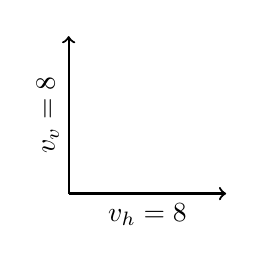
\begin{tikzpicture}
                \draw[white] (-0.5,-0.5) rectangle (2.1,2.1);
                \draw[thick,->] (0,0) -- (90:2cm);
                \node[anchor=south,rotate=90] at (90:1cm) {$v_v=\SI{8}{\meter\per\second}$};
                \draw[thick,->] (0,0) -- (0:2cm);
                \node[anchor=north] at (0:1cm) {$v_h=\SI{8}{\meter\per\second}$};
            \end{tikzpicture}
        }
        \wrongchoice{
            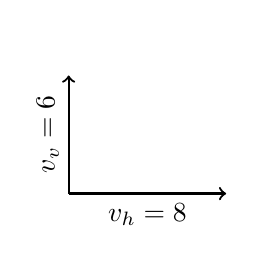
\begin{tikzpicture}
                \draw[white] (-0.5,-0.5) rectangle (2.1,2.1);
                \draw[thick,->] (0,0) -- (90:1.5cm);
                \node[anchor=south,rotate=90] at (90:0.75cm) {$v_v=\SI{6}{\meter\per\second}$};
                \draw[thick,->] (0,0) -- (0:2cm);
                \node[anchor=north] at (0:1cm) {$v_h=\SI{8}{\meter\per\second}$};
            \end{tikzpicture}
        }
        \wrongchoice{
            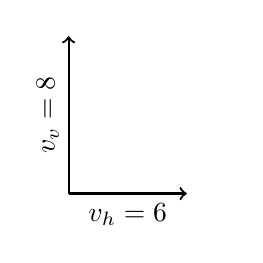
\begin{tikzpicture}
                \draw[white] (-0.5,-0.5) rectangle (2.1,2.1);
                \draw[thick,->] (0,0) -- (90:2cm);
                \node[anchor=south,rotate=90] at (90:1cm) {$v_v=\SI{8}{\meter\per\second}$};
                \draw[thick,->] (0,0) -- (0:1.5cm);
                \node[anchor=north] at (0:0.75cm) {$v_h=\SI{6}{\meter\per\second}$};
            \end{tikzpicture}
        }
        \wrongchoice{
            \begin{tikzpicture}
                \draw[white] (-0.5,-0.5) rectangle (2.1,2.1);
                \draw[thick,->] (0,0) -- (90:1.5cm);
                \node[anchor=south,rotate=90] at (90:0.75cm) {$v_v=\SI{6}{\meter\per\second}$};
                \draw[thick,->] (0,0) -- (0:1.5cm);
                \node[anchor=north] at (0:0.75cm) {$v_h=\SI{6}{\meter\per\second}$};
            \end{tikzpicture}
        }
    \end{choices}
    \end{multicols}
\end{question}
}


%% Section June2013
%%--------------------
\element{nysed}{
\begin{question}{June2013-Q05}
    A projectile is launched at an angle above the ground.
    The horizontal component of the projectile's velocity, $v_x$, is initially \SI{40}{\meter\per\second}.
    The vertical component of the projectile's velocity, $v_y$, is initially \SI{30}{\meter\per\second}.
    What are the components of the projectile's velocity after \SI{2.0}{\second} of flight?
    [Neglect friction.]
    \begin{choices}
      \correctchoice{$v_x=\SI{40}{\meter\per\second}$ and $v_y=\SI{10}{\meter\per\second}$}
        \wrongchoice{$v_x=\SI{40}{\meter\per\second}$ and $v_y=\SI{30}{\meter\per\second}$}
        \wrongchoice{$v_x=\SI{20}{\meter\per\second}$ and $v_y=\SI{10}{\meter\per\second}$}
        \wrongchoice{$v_x=\SI{20}{\meter\per\second}$ and $v_y=\SI{30}{\meter\per\second}$}
    \end{choices}
\end{question}
}

\element{nysed}{
\begin{question}{June2013-Q06}
    A ball is thrown with an initial speed of \SI{10}{\meter\per\second}.
    At what angle above the horizontal should the ball be thrown to reach the greatest height?
    \begin{multicols}{4}
    \begin{choices}
        \wrongchoice{\ang{0}}
        \wrongchoice{\ang{30}}
        \wrongchoice{\ang{45}}
      \correctchoice{\ang{90}}
    \end{choices}
    \end{multicols}
\end{question}
}


%% Section June2012
%%--------------------
\element{nysed}{
\begin{question}{June2012-Q45}
    The diagram below represents a setup for demonstrating motion.
    \begin{center}
        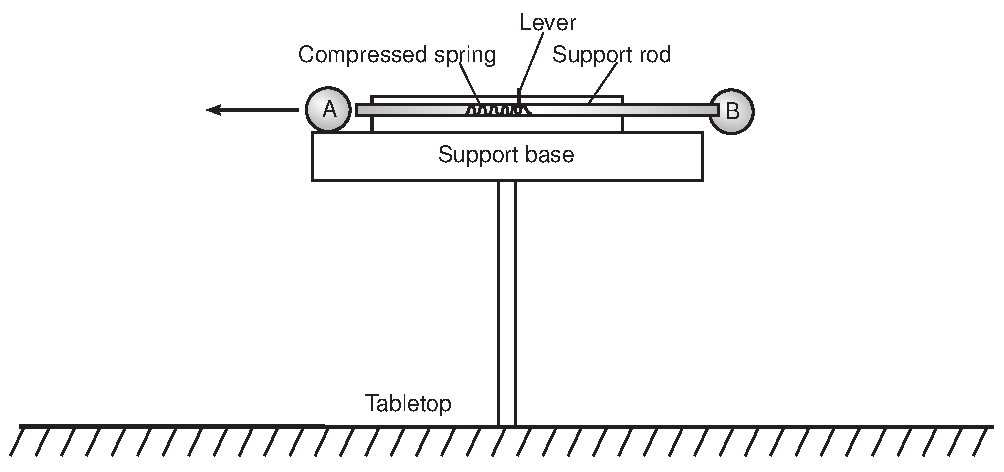
\includegraphics[keepaspectratio,width=0.95\linewidth]{June2012-Q45}
    \end{center}
    When the lever is released, the support rod withdraws from ball $A$, allowing it to fall.
    At the same instant, the rod contacts ball $A$, propelling it horizontally to the left.
    Which statement describes the motion that is observed after the lever is released and the balls fall?
    [Neglect friction.]
    \begin{choices}
        \wrongchoice{Ball $A$ travels at constant velocity.}
      \correctchoice{Ball $A$ hits the tabletop at the same times as ball $B$.}
        \wrongchoice{Ball $B$ hits the tabletop before ball $A$.}
        \wrongchoice{Ball $B$ travels with an increasing acceleration.}
    \end{choices}
\end{question}
}


%% Section June2011
%%--------------------
\element{nysed}{
\begin{question}{June2011-Q11}
    Four identical projectiles are launched with the same initial speed, $v$,
        but at various angles above the level ground.
    Which diagram represents the initial velocity of the projectile that will have the largest total horizontal displacement?
    [Neglect air resistance.]
    \begin{multicols}{2}
    \begin{choices}
        \AMCboxDimensions{down=-1.5em}
        \wrongchoice{
            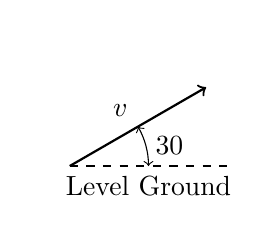
\begin{tikzpicture}
                \draw[white] (-1.5em,-1.5em) rectangle (2,1.75);
                \draw[dashed] (0,0) -- (2,0) node[pos=0.5,anchor=north] {Level Ground};
                \draw[thick,->] (0,0) -- (30:2) node[pos=0.5,anchor=south east] {$v$};
                \draw[<->] (1,0) arc (0:30:1) node[pos=0.5,anchor=west] {\ang{30}};
            \end{tikzpicture}
        }
        \correctchoice{
            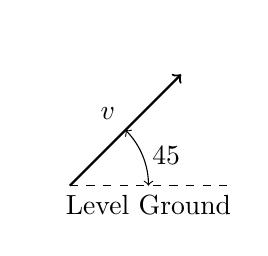
\begin{tikzpicture}
                \draw[white] (-1.5em,-1.5em) rectangle (2,2);
                \draw[dashed] (0,0) -- (2,0) node[pos=0.5,anchor=north] {Level Ground};
                \draw[thick,->] (0,0) -- (45:2) node[pos=0.5,anchor=south east] {$v$};
                \draw[<->] (1,0) arc (0:45:1) node[pos=0.5,anchor=west] {\ang{45}};
            \end{tikzpicture}
        }
        \wrongchoice{
            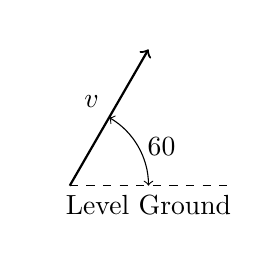
\begin{tikzpicture}
                \draw[white] (-1.5em,-1.5em) rectangle (2,2);
                \draw[dashed] (0,0) -- (2,0) node[pos=0.5,anchor=north] {Level Ground};
                \draw[thick,->] (0,0) -- (60:2) node[pos=0.5,anchor=south east] {$v$};
                \draw[<->] (1,0) arc (0:60:1) node[pos=0.5,anchor=west] {\ang{60}};
            \end{tikzpicture}
        }
        \wrongchoice{
            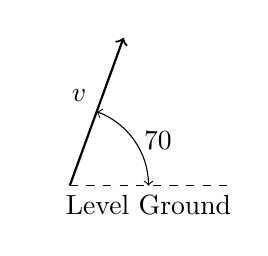
\begin{tikzpicture}
                \draw[white] (-1.5em,-1.5em) rectangle (2,2);
                \draw[dashed] (0,0) -- (2,0) node[pos=0.5,anchor=north] {Level Ground};
                \draw[thick,->] (0,0) -- (70:2) node[pos=0.5,anchor=south east] {$v$};
                \draw[<->] (1,0) arc (0:70:1) node[pos=0.5,anchor=west] {\ang{70}};
            \end{tikzpicture}
        }
    \end{choices}
    \end{multicols}
\end{question}
}


%% Section June2010
%%--------------------
\element{nysed}{
\begin{question}{June2010-Q06}
    As shown in the diagram below,
        a student standing on the roof of a \SI{50.0}{\meter} high building kicks a stone at a horizontal speed of \SI{4.00}{\meter\per\second}.
    \begin{center}
    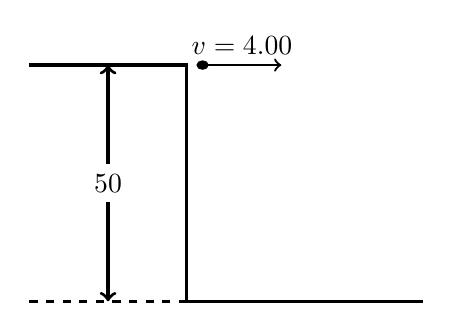
\begin{tikzpicture}[yscale=0.75]
        \draw[very thick] (-2,0) -- (0,0) -- (0,-4) -- (3,-4);
        \draw[fill] (0.2,0.0) circle [radius=2pt];
        \draw[thick,->] (0.2,0.0) -- ++ (0:1)
            node[anchor=south] at ++ (0:-0.5) {$v=\SI{4.00}{\meter\per\second}$};
        \draw[very thick,dashed] (-2,-4) -- (0,-4);
        \node (A) at (-1,-2.0) {\SI{50}{\meter}};
        \draw[very thick,->] (A) -- (-1,0);
        \draw[very thick,->] (A) -- (-1,-4);
    \end{tikzpicture}
    \end{center}
    How much time is required for the stone to reach the level ground below?
    [Neglect friction.]
    \begin{multicols}{2}
    \begin{choices}
      \correctchoice{\SI{3.19}{\second}}
        \wrongchoice{\SI{5.10}{\second}}
        \wrongchoice{\SI{10.2}{\second}}
        \wrongchoice{\SI{12.5}{\second}}
    \end{choices}
    \end{multicols}
\end{question}
}

\element{nysed}{
\begin{question}{June2010-Q14}
    Four projectiles, $I$, $J$, $K$, and $L$,
        were launched from, and returned to, level ground.
    The data table below shows the initial horizontal speed,
        initial vertical speed, and time of flights for each projectile.
    Which projectile traveled the greatest horizontal distance?
    [Neglect friction.]
    \begin{center}
    \begin{tabu}{cX[c]X[c]X[c]}
        \toprule
        \makebox[1.5em][c]{\textnumero} &
        Initial Horizontal Speed [\si{\meter\per\second}] &
        Initial Vertical Speed [\si{\meter\per\second}] &
        Time of Flight [\si{\second}] \\
        \bottomrule
    \end{tabu}
    \end{center}
    \begin{choices}
        \wrongchoice{\begin{tabu}{X[c]X[c]X[c]} 40.0 & 29.4 & 6.00 \\ \end{tabu}}
        \wrongchoice{\begin{tabu}{X[c]X[c]X[c]} 60.0 & 19.6 & 4.00 \\ \end{tabu}}
        \wrongchoice{\begin{tabu}{X[c]X[c]X[c]} 50.0 & 24.5 & 5.00 \\ \end{tabu}}
      \correctchoice{\begin{tabu}{X[c]X[c]X[c]} 80.0 & 19.6 & 4.00 \\ \end{tabu}}
    \end{choices}
\end{question}
}


\element{nysed}{
\begin{question}{June2010-Q42}
    A student throws a baseball vertically upward and then catches it.
    If vertically upward is considered to be the positive direction,
        which graph best represents the relationship between velocity and time for the baseball?
    [Neglect friction.]
    \begin{multicols}{2}
    \begin{choices}
        \AMCboxDimensions{down=-1.5em}
        \correctchoice{
            \begin{tikzpicture}
                \begin{axis}[
                    axis y line=left,
                    axis x line=middle,
                    axis line style={->},
                    xlabel={time},
                    xtick=\empty,
                    ylabel={velocity},
                    ytick=\empty,
                    xmin=0,xmax=11,
                    ymin=-5,ymax=6,
                    width=0.95\columnwidth,
                    very thin,
                ]
                \addplot[line width=1pt,domain=0:10]{5-x};
                \end{axis}
            \end{tikzpicture}
        }
        \wrongchoice{
            \begin{tikzpicture}
                \begin{axis}[
                    axis y line=left,
                    axis x line=middle,
                    axis line style={->},
                    xlabel={time},
                    xtick=\empty,
                    x label style={anchor=north east},
                    ylabel={velocity},
                    ytick=\empty,
                    xmin=0,xmax=11,
                    ymin=-5,ymax=6,
                    width=0.95\columnwidth,
                    very thin,
                ]
                \addplot[line width=1pt,domain=0:5]{x};
                \addplot[line width=1pt,domain=5:10]{10-x};
                \end{axis}
            \end{tikzpicture}
        }
        \wrongchoice{
            \begin{tikzpicture}
                \begin{axis}[
                    axis y line=left,
                    axis x line=middle,
                    axis line style={->},
                    xlabel={time},
                    xtick=\empty,
                    x label style={anchor=north east},
                    ylabel={velocity},
                    ytick=\empty,
                    xmin=0,xmax=11,
                    ymin=-5,ymax=6,
                    width=0.95\columnwidth,
                    very thin,
                ]
                \addplot[line width=1pt,domain=0:10]{-0.20*x*(x-10)};
                \end{axis}
            \end{tikzpicture}
        }
        \wrongchoice{
            \begin{tikzpicture}
                \begin{axis}[
                    axis y line=left,
                    axis x line=middle,
                    axis line style={->},
                    xlabel={time},
                    xtick=\empty,
                    x label style={anchor=north east},
                    ylabel={velocity},
                    ytick=\empty,
                    xmin=0,xmax=11,
                    ymin=-5,ymax=6,
                    width=0.95\columnwidth,
                    very thin,
                ]
                \addplot[line width=1pt,domain=0:5]{5-x};
                \addplot[line width=1pt,domain=5:10]{-5+x};
                \end{axis}
            \end{tikzpicture}
        }
    \end{choices}
    \end{multicols}
\end{question}
}


%% Section June2009
%%--------------------
\element{nysed}{
\begin{question}{June2009-Q06}
    A golf ball is given an initial speed of \SI{20}{\meter\per\second} and returns to level ground.
    Which launch angle above level ground results in the ball traveling the greatest distance?
    [Neglect friction.]
    \begin{multicols}{4}
    \begin{choices}
        \wrongchoice{\ang{60}}
      \correctchoice{\ang{45}}
        \wrongchoice{\ang{30}}
        \wrongchoice{\ang{15}}
    \end{choices}
    \end{multicols}
\end{question}
}


%% Section Jan2009
%%--------------------
\element{nysed}{
\begin{question}{Jan2009-Q08}
    The diagram below represents the path of a stunt car that is driven off a cliff,
        neglecting friction.
    \begin{center}
    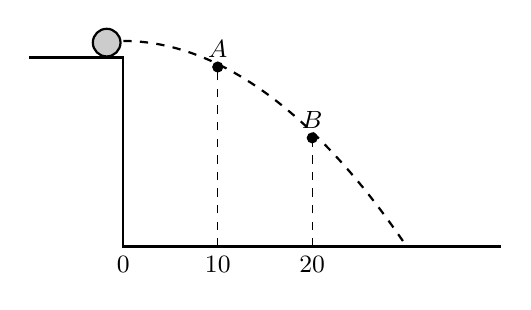
\begin{tikzpicture}[font=\small,scale=1.2]
        %% Surface
        \draw[thick] (-1,0) -- (0,0) -- (0,-2) -- (4,-2);
        %% Labels: 0 m 
        \node[anchor=north] at (0,-2) {\SI{0}{\meter}};
        \draw[fill] (1,-0.1) circle (1.5pt) node[anchor=south] {$A$};
        %% Labels: A at 10 m 
        \draw[dashed] (1,-2) -- (1,-0.1);
        \node[anchor=north] at (1,-2) {\SI{10}{\meter}};
        %% Labels: B at 20 m 
        \draw[fill] (2,-0.85) circle (1.5pt) node[anchor=south] {$B$};
        \draw[dashed] (2,-2) -- (2,-0.85);
        \node[anchor=north] at (2,-2) {\SI{20}{\meter}};
        %% Path
        \node[thick,draw,fill=white!80!black,anchor=south,circle,minimum size=1em] (Car) at (-0.5em,0) {};
        %\draw[->] (Car.east) -- ++ (0:0.75cm) node[pos=0.5,anchor=south] {$v$};
        \draw[thick,dashed] (0,0.5em) parabola bend (0,0.5em) (3,-2);
    \end{tikzpicture}
    \end{center}
    Compared to the horizontal component of the car's velocity at point $A$,
        the horizontal component of the car's velocity at point $B$ is:
    \begin{multicols}{3}
    \begin{choices}
        \wrongchoice{smaller}
        \wrongchoice{greater}
      \correctchoice{the same}
    \end{choices}
    \end{multicols}
\end{question}
}


%% Section June2008
%%--------------------
\element{nysed}{
\begin{question}{June2008-Q02}
    A projectile launched at an angle of \ang{45} above the horizontal travels through the air.
    Compared to the projectile's theoretical path with no air friction,
        the actual trajectory of the projectile with air friction is:
    \begin{choices}
      \correctchoice{lower and shorter}
        \wrongchoice{lower and longer}
        \wrongchoice{higher and shorter}
        \wrongchoice{higher and longer}
    \end{choices}
\end{question}
}

\element{nysed}{
\begin{question}{June2008-Q06}
    Two stones, $A$ and $B$, are thrown horizontally from the top of a cliff.
    Stone $A$ has an initial speed of \SI{15}{\meter\per\second} and stone $B$ has an initial speed of \SI{30}{\meter\per\second}.
    Compared to the time it takes stone $A$ to reach the ground,
        the time it takes stone $B$ to reach the ground is:
    \begin{choices}
      \correctchoice{the same}
        \wrongchoice{twice as great}
        \wrongchoice{half as great}
        \wrongchoice{four times as great}
    \end{choices}
\end{question}
}


%% Section Jan2008
%%--------------------
\element{nysed}{
\begin{question}{Jan2008-Q07}
    Two spheres, $A$ and $B$, are simultaneously projected horizontally from the top of a tower.
    Sphere $A$ has a horizontal speed of \SI{40}{\meter\per\second} and sphere $B$ has a horizontal speed of \SI{20}{\meter\per\second}.
    Which statement best describes the time required for the spheres to reach the ground and the horizontal distance they travel?
    [Neglect friction and assume the ground is level.]
    \begin{choices}
        \wrongchoice{Both spheres hit the ground at the same time and at the same distance from the base of the tower}
      \correctchoice{Both spheres hit the ground at the same time, but sphere $A$ lands twice as far as sphere $B$ from the base of the tower.}
        \wrongchoice{Both spheres hit the ground at the same time, but sphere $B$ lands twice as far as sphere $A$ from the base of the tower.}
        \wrongchoice{Sphere $A$ hits the ground before sphere $B$, and sphere $A$ lands twice as far as sphere $B$ from the base of the tower.}
    \end{choices}
\end{question}
}


%% Section June2007
%%--------------------


%% Section Jan2007
%%--------------------
\element{nysed}{
\begin{question}{Jan2007-Q05}
    A machine launches a tennis ball at an angle of \ang{25} above the horizontal at a speed of \SI{14}{\meter\per\second}.
    The ball returns to level ground.
    Which combination of changes \emph{must} produce an increase in time of flight of a second launch?
    \begin{choices}
      \correctchoice{increase the launch angle and increase the ball's initial speed}
        \wrongchoice{increase the launch angle and decrease the ball's initial speed}
        \wrongchoice{decrease the launch angle and increase the ball's initial speed}
        \wrongchoice{decrease the launch angle and decrease the ball's initial speed}
    \end{choices}
\end{question}
}

\element{nysed}{
\begin{question}{Jan2007-Q07}
    A plane flying horizontally above Earth's surface at \SI{100}{\meter\per\second} drops a crate.
    The crate strikes the ground \SI{30.0}{\second} later.
    What is the magnitude of the horizontal component of the crate's velocity just before it strikes the ground?
    [Neglect friction.]
    \begin{multicols}{2}
    \begin{choices}
      \correctchoice{\SI{100}{\meter\per\second}}
        \wrongchoice{\SI{0}{\meter\per\second}}
        \wrongchoice{\SI{294}{\meter\per\second}}
        \wrongchoice{\SI{394}{\meter\per\second}}
    \end{choices}
    \end{multicols}
\end{question}
}


%% Section June2006
%%--------------------
\element{nysed}{
\begin{question}{June2006-Q44}
    A volleyball hit into the air has an initial speed of \SI{10.}{\meter\per\second}.
    Which vector best represents the angle above the horizontal that the ball should be hit to remain in the air for the greatest amount of time?
    \begin{multicols}{2}
    \begin{choices}
        \AMCboxDimensions{down=-1.5em}
        \correctchoice{
            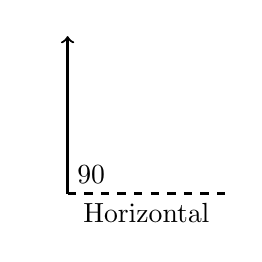
\begin{tikzpicture}
                \draw[white] (-0.5,-0.5) rectangle (2.1,2.1);
                \draw[thick,->] (0,0) -- (90:2cm);
                \draw[thick,dashed] (0,0) -- (0:2cm);
                \node[anchor=north] at (0:1cm) {Horizontal};
                \node[anchor=south west] at (0:0) {\ang{90}};
            \end{tikzpicture}
        }
        \wrongchoice{
            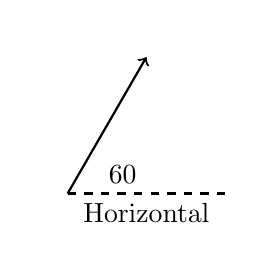
\begin{tikzpicture}
                \draw[white] (-0.5,-0.5) rectangle (2.1,2.1);
                \draw[thick,->] (0,0) -- (60:2cm);
                \draw[thick,dashed] (0,0) -- (0:2cm);
                \node[anchor=north] at (0:1cm) {Horizontal};
                \node[anchor=south east] at (0:1cm) {\ang{60}};
            \end{tikzpicture}
        }
        \wrongchoice{
            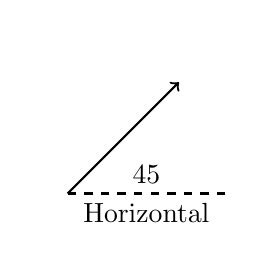
\begin{tikzpicture}
                \draw[white] (-0.5,-0.5) rectangle (2.1,2.1);
                \draw[thick,->] (0,0) -- (45:2cm);
                \draw[thick,dashed] (0,0) -- (0:2cm);
                \node[anchor=north] at (0:1cm) {Horizontal};
                \node[anchor=south] at (0:1cm) {\ang{45}};
            \end{tikzpicture}
        }
        \wrongchoice{
            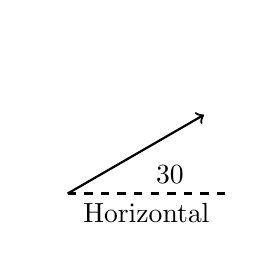
\begin{tikzpicture}
                \draw[white] (-0.5,-0.5) rectangle (2.1,2.1);
                \draw[thick,->] (0,0) -- (30:2cm);
                \draw[thick,dashed] (0,0) -- (0:2cm);
                \node[anchor=north] at (0:1cm) {Horizontal};
                \node[anchor=south west] at (0:1cm) {\ang{30}};
            \end{tikzpicture}
        }
    \end{choices}
    \end{multicols}
\end{question}
}


%% Section Jan2006
%%--------------------


%% Section June2005
%%--------------------
\element{nysed}{
\begin{question}{June2005-Q05}
    A golf ball is hit at an angle of \ang{45} above the horizontal.
    What is the acceleration of the gold ball at the highest point in its trajectory?
    [Neglect friction.]
    \begin{choices}
      \correctchoice{\SI{9.8}{\meter\per\second\squared} downward}
        \wrongchoice{\SI{9.8}{\meter\per\second\squared} upward}
        \wrongchoice{\SI{6.9}{\meter\per\second\squared} horizontal}
        \wrongchoice{\SI{0.0}{\meter\per\second\squared}}
    \end{choices}
\end{question}
}

\element{nysed}{
\begin{question}{June2005-Q07}
    A ball is thrown horizontally at a speed of \SI{24}{\meter\per\second} from the top of a cliff.
    If the ball hits the ground \SI{4.0}{\second} later,
        approximately how high is the cliff?
    \begin{multicols}{2}
    \begin{choices}
      \correctchoice{\SI{78}{\meter}}
        \wrongchoice{\SI{96}{\meter}}
        \wrongchoice{\SI{6.0}{\meter}}
        \wrongchoice{\SI{39}{\meter}}
    \end{choices}
    \end{multicols}
\end{question}
}


%% Section Jan2005
%%--------------------


%% Section June2004
%%--------------------
\element{nysed}{
\begin{question}{June2004-Q04}
    The diagram below represents the path of an object after it was thrown.
    \begin{center}
    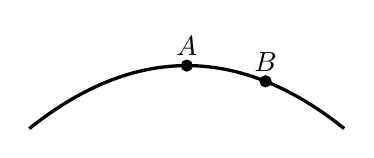
\begin{tikzpicture}
        \draw [very thick,domain=-2:2, samples=50] plot (\x, {2 - 0.20*\x*\x});
        \node [anchor=south] at (0,2) {$A$};
        \draw[fill] (0,2) circle (2pt);
        \node [anchor=south] at (1,1.80) {$B$};
        \draw[fill] (1,1.80) circle (2pt);
    \end{tikzpicture}
    \end{center}
    What happens to the object's acceleration as it travels from $A$ to $B$?
    [Neglect friction.]
    \begin{choices}
      \correctchoice{It remains the same}
        \wrongchoice{It increases}
        \wrongchoice{It decreases}
    \end{choices}
\end{question}
}

\element{nysed}{
\begin{question}{June2004-Q05}
    A \SI{0.2}{\kilo\gram} red ball is thrown horizontally at a speed of \SI{4}{\meter\per\second} from a height of \SI{3}{\meter}.
    A \SI{0.4}{\kilo\gram} green ball is thrown horizontally from the same height at a speed of \SI{8}{\meter\per\second}.
    Compared to the time it takes the red ball to reach the ground,
        the time it takes the green ball to reach the ground is:
    \begin{choices}
      \correctchoice{the same}
        \wrongchoice{one-half as great}
        \wrongchoice{twice as great}
        \wrongchoice{four times as great}
    \end{choices}
\end{question}
}


%% Section Jan2004
%%--------------------
\element{nysed}{
\begin{question}{Jan2004-Q06}
    A child kicks a ball with an initial velocity of \SI{8.5}{\meter\per\second} at an angle of \ang{35} with the horizontal,
        as shown.
    The ball has an initial velocity of \SI{4.9}{\meter\per\second} and a total time of flight of \SI{1.0}{\second}.
    [Neglect air resistance.]
    \begin{center}
        %% Part I of two part question
        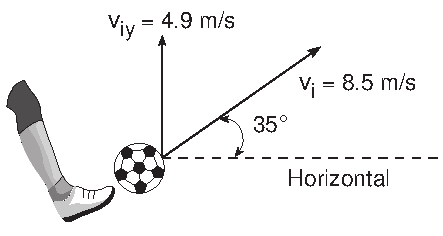
\includegraphics[keepaspectratio,width=0.80\linewidth]{Jan2004-Q06}
    \end{center}
    The horizontal component of the ball's initial velocity is approximately
    \begin{multicols}{2}
    \begin{choices}
      \correctchoice{\SI{7.0}{\meter\per\second}}
        \wrongchoice{\SI{13}{\meter\per\second}}
        \wrongchoice{\SI{3.6}{\meter\per\second}}
        \wrongchoice{\SI{4.9}{\meter\per\second}}
    \end{choices}
    \end{multicols}
\end{question}
}

\element{nysed}{
\begin{question}{Jan2004-Q07}
    A child kicks a ball with an initial velocity of \SI{8.5}{\meter\per\second} at an angle of \ang{35} with the horizontal,
        as shown.
    The ball has an initial velocity of \SI{4.9}{\meter\per\second} and a total time of flight of \SI{1.0}{\second}.
    [Neglect air resistance.]
    \begin{center}
        %% Part II of two part question
        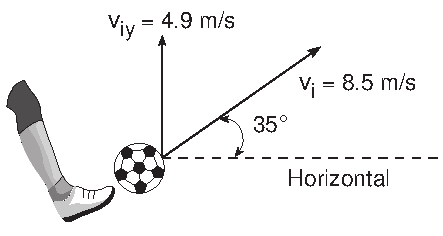
\includegraphics[keepaspectratio,width=0.80\linewidth]{Jan2004-Q06}
    \end{center}
    The maximum height reached by the ball is approximately:
    \begin{multicols}{2}
    \begin{choices}
      \correctchoice{\SI{1.2}{\meter}}
        \wrongchoice{\SI{2.5}{\meter}}
        \wrongchoice{\SI{4.9}{\meter}}
        \wrongchoice{\SI{8.5}{\meter}}
    \end{choices}
    \end{multicols}
\end{question}
}


%% Section June2003
%%--------------------
\element{nysed}{
\begin{question}{June2003-Q04}
    A ball is thrown at an angle of \ang{33} to the horizontal.
    What happens to the magnitude of the ball's vertical acceleration during the total time interval that the ball is in the air?
    \begin{choices}
        \wrongchoice{It decreases, then increases}
        \wrongchoice{It decreases, then remains the same}
        \wrongchoice{It increases, then decreases}
      \correctchoice{It remains the same}
    \end{choices}
\end{question}
}

\element{nysed}{
\begin{question}{June2003-Q06}
    Projectile A is launched horizontally at a speed of \SI{20}{\meter\per\second} from the top of a cliff and strikes a level surface below,
        \SI{3.0}{\second} later.
    Projectile B is launched horizontally from the same location at a speed of \SI{30}{\meter\per\second}.
    The time it takes projectile B to reach the level surface is:
    \begin{multicols}{2}
    \begin{choices}
      \correctchoice{\SI{3.0}{\second}}
        \wrongchoice{\SI{4.5}{\second}}
        \wrongchoice{\SI{2.0}{\second}}
        \wrongchoice{\SI{10}{\second}}
    \end{choices}
    \end{multicols}
\end{question}
}

\element{nysed}{
\begin{question}{June2003-Q07}
    Projectile A is launched horizontally at a speed of \SI{20}{\meter\per\second} from the top of a cliff and strikes a level surface below,
        \SI{3.0}{\second} later.
    Projectile B is launched horizontally from the same location at a speed of \SI{30}{\meter\per\second}.
    Approximately how high is the cliff?
    \begin{multicols}{2}
    \begin{choices}
      \correctchoice{\SI{44}{\meter}}
        \wrongchoice{\SI{29}{\meter}}
        \wrongchoice{\SI{60}{\meter}}
        \wrongchoice{\SI{104}{\meter}}
    \end{choices}
    \end{multicols}
\end{question}
}


%% Section Jan2003
%%--------------------


%% Section Aug2002
%%--------------------
\element{nysed}{
\begin{question}{Aug2002-Q38}
    An archer uses a bow to fire two similar arrows with the same string force.
    One arrow is fired at an angle of \ang{60} with the horizontal,
        and the other is fired at an angle of \ang{45} with the horizontal.
    Compared to the arrow fired at \ang{60},
        the arrow fired at \ang{45} has a:
    \begin{choices}
        \wrongchoice{longer flight time and longer horizontal range}
        \wrongchoice{longer flight time and shorter horizontal range}
      \correctchoice{shorter flight time and longer horizontal range}
        \wrongchoice{shorter flight time and shorter horizontal range}
    \end{choices}
\end{question}
}



%% Section June2002
%%--------------------
\element{nysed}{
\begin{question}{June2002-Q05}
    The diagram below shows a student throwing a baseball horizontally at \SI{25}{\meter\per\second} from a cliff \SI{45}{\meter} above the level ground.
    \begin{center}
    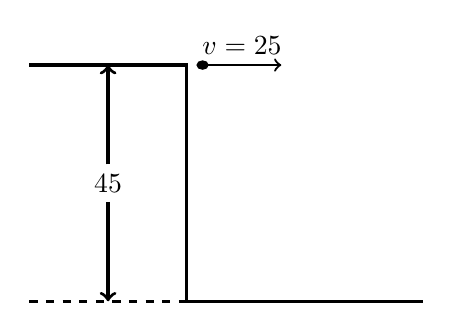
\begin{tikzpicture}[yscale=0.75]
        \draw[very thick] (-2,0) -- (0,0) -- (0,-4) -- (3,-4);
        \draw[fill] (0.2,0.0) circle [radius=2pt];
        \draw[thick,->] (0.2,0.0) -- ++ (0:1)
            node[anchor=south] at ++ (0:-0.5) {$v=\SI{25}{\meter\per\second}$};
        \draw[very thick,dashed] (-2,-4) -- (0,-4);
        \node (A) at (-1,-2.0) {\SI{45}{\meter}};
        \draw[very thick,->] (A) -- (-1,0);
        \draw[very thick,->] (A) -- (-1,-4);
    \end{tikzpicture}
    \end{center}
    Approximately how far from the base of the cliff does the ball hit the ground?
    [Neglect air resistance]
    \begin{multicols}{2}
    \begin{choices}
        \wrongchoice{\SI{45}{\meter}}
      \correctchoice{\SI{75}{\meter}}
        \wrongchoice{\SI{140}{\meter}}
        \wrongchoice{\SI{230}{\meter}}
    \end{choices}
    \end{multicols}
\end{question}
}

\element{nysed}{
\begin{question}{June2002-Q06}
    A projectile is fired from a gun near the surface of Earth.
    The initial velocity of the projectile has a vertical component of \SI{98}{\meter\per\second} and a horizontal component of \SI{49}{\meter\per\second}.
    How long will it take the projectile to reach the highest point in its path?
    \begin{multicols}{2}
    \begin{choices}
        \wrongchoice{\SI{5.0}{\second}}
        \wrongchoice{\SI{10}{\second}}
        \wrongchoice{\SI{20}{\second}}
      \correctchoice{\SI{100}{\second}}
    \end{choices}
    \end{multicols}
\end{question}
}


%% Section Jan2002
%%--------------------
\element{nysed}{
\begin{question}{Jan2002-Q06}
    Which two terms represent a vector quantity and the scalar quantity of the vector's magnitude respectively?
    \begin{choices}
        \wrongchoice{acceleration and velocity}
        \wrongchoice{weight and force}
        \wrongchoice{speed and time}
      \correctchoice{displacement and distance}
    \end{choices}
\end{question}
}
 
\element{nysed}{
\begin{question}{Jan2002-Q07}
    A \SI{4.0}{\kilo\gram} rock and a \SI{1.0}{\kilo\gram} stone fall freely from rest from a height of \SI{100}{\meter}.
    After they fall for \SI{2.0}{\second},
        the ratio of the rock's speed to the stone's speed is:
    \begin{multicols}{2}
    \begin{choices}
      \correctchoice{$1:1$}
        \wrongchoice{$1:2$}
        \wrongchoice{$2:1$}
        \wrongchoice{$4:1$}
    \end{choices}
    \end{multicols}
\end{question}
}

\element{nysed}{
\begin{question}{Jan2002-Q56}
    A ball is thrown horizontally with an initial velocity of \SI{20.0}{\meter\per\second} from the top of a tower \SI{60.0}{\meter} high.
    \begin{center}
        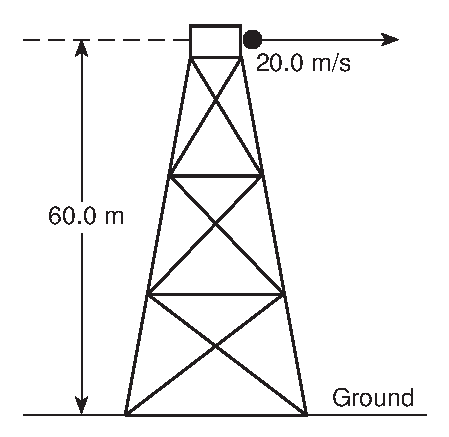
\includegraphics[keepaspectratio,scale=0.95]{Jan2002-Q56}
    \end{center}
    What is the initial vertical velocity of the ball?
    \begin{multicols}{2}
    \begin{choices}
      \correctchoice{\SI{0}{\meter\per\second}}
        \wrongchoice{\SI{9.81}{\meter\per\second}}
        \wrongchoice{\SI{20.0}{\meter\per\second}}
        \wrongchoice{\SI{60.0}{\meter\per\second}}
    \end{choices}
    \end{multicols}
\end{question}
}

\element{nysed}{
\begin{question}{Jan2002-Q57}
    A ball is thrown horizontally with an initial velocity of \SI{20.0}{\meter\per\second} from the top of a tower \SI{60.0}{\meter} high.
    \begin{center}
        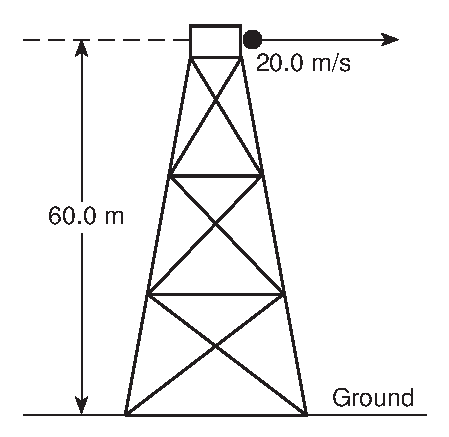
\includegraphics[keepaspectratio,scale=0.95]{Jan2002-Q56}
    \end{center}
    What is the approximate total time required for the ball to reach the ground?
    [Neglect air resistance]
    \begin{multicols}{2}
    \begin{choices}
        \wrongchoice{\SI{12.2}{\second}}
        \wrongchoice{\SI{2.04}{\second}}
        \wrongchoice{\SI{3.00}{\second}}
      \correctchoice{\SI{3.50}{\second}}
    \end{choices}
    \end{multicols}
\end{question}
}

\element{nysed}{
\begin{question}{Jan2002-Q58}
    A ball is thrown horizontally with an initial velocity of \SI{20.0}{\meter\per\second} from the top of a tower \SI{60.0}{\meter} high.
    \begin{center}
        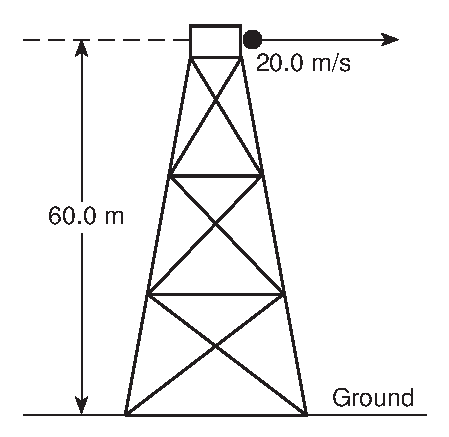
\includegraphics[keepaspectratio,scale=0.95]{Jan2002-Q56}
    \end{center}
    What is the horizontal velocity of the ball just before it reaches the ground?
    [Neglect air resistance.]
    \begin{multicols}{2}
    \begin{choices}
        \wrongchoice{\SI{9.81}{\meter\per\second}}
      \correctchoice{\SI{20.0}{\meter\per\second}}
        \wrongchoice{\SI{34.3}{\meter\per\second}}
        \wrongchoice{\SI{68.6}{\meter\per\second}}
    \end{choices}
    \end{multicols}
\end{question}
}

\element{nysed}{
\begin{question}{Jan2002-Q62}
    A golf ball leaves a golf club with an initial velocity of \SI{40}{\meter\per\second} at an angle of \ang{40} with respect to the horizontal.
    \begin{center}
        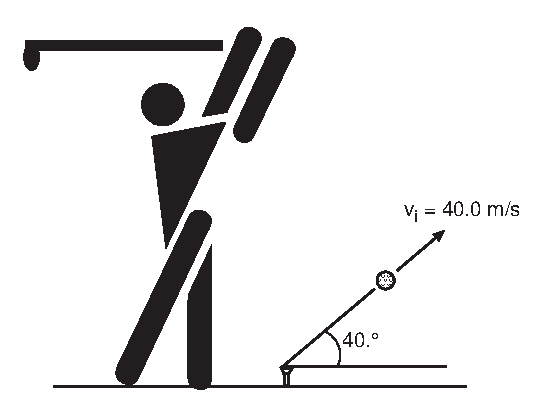
\includegraphics[keepaspectratio,scale=0.90]{Jan2002-Q62}
    \end{center}
    What is the vertical component of the golf ball's initial velocity?
    \begin{multicols}{2}
    \begin{choices}
      \correctchoice{\SI{25.7}{\meter\per\second}}
        \wrongchoice{\SI{30.6}{\meter\per\second}}
        \wrongchoice{\SI{40.0}{\meter\per\second}}
        \wrongchoice{\SI{61.3}{\meter\per\second}}
    \end{choices}
    \end{multicols}
\end{question}
}

\element{nysed}{
\begin{question}{Jan2002-Q63}
    A golf ball leaves a golf club with an initial velocity of \SI{40}{\meter\per\second} at an angle of \ang{40} with respect to the horizontal.
    \begin{center}
        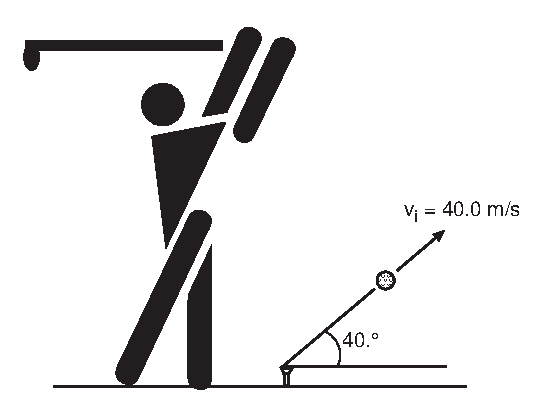
\includegraphics[keepaspectratio,scale=0.90]{Jan2002-Q62}
    \end{center}
    What is the total horizontal distance traveled by the golf ball during the first \SI{2.5}{\second} of its flight?
    \begin{multicols}{2}
    \begin{choices}
        \wrongchoice{\SI{100}{\meter}}
      \correctchoice{\SI{76.6}{\meter}}
        \wrongchoice{\SI{64.3}{\meter}}
        \wrongchoice{\SI{40.0}{\meter}}
    \end{choices}
    \end{multicols}
\end{question}
}


%% Section June2001
%%--------------------
\element{nysed}{
\begin{question}{June2001-Q58}
    A red ball and a green ball are simultaneously thrown horizontally from the same height.
    The red ball has an initial speed of \SI{40}{\meter\per\second} and the green ball has an initial speed of \SI{20}{\meter\per\second}.
    Compared to the time it takes the red ball to reach the ground,
        the time it takes the green ball to reach the ground will be:
    \begin{choices}
      \correctchoice{the same}
        \wrongchoice{half as much}
        \wrongchoice{twice as much}
        \wrongchoice{four times as much}
    \end{choices}
\end{question}
}

\element{nysed}{
\begin{question}{June2001-Q59}
    A baseball player throws a ball horizontally.
    Which statement best describes the ball's motion after it is thrown?
    [Neglect the effect of friction.]
    \begin{choices}
        \wrongchoice{Its vertical speed remains the same, and its horizontal speed increases.}
        \wrongchoice{Its vertical speed remains the same, and its horizontal speed remains the same.}
        \wrongchoice{Its vertical speed increases, and its horizontal speed increases.}
      \correctchoice{Its vertical speed increases, and its horizontal speed remains the same.}
    \end{choices}
\end{question}
}


%% Section Jan2001
%%--------------------
\element{nysed}{
\begin{question}{Jan2001-Q58}
    A red ball and a green ball are simultaneously thrown horizontally from the same height.
    the red ball has an initial speed of \SI{40}{\meter\per\second} and the green ball has an initial speed of \SI{20}{\meter\per\second}.
    Compared to the the time it takes the red ball to reach the ground,
        the time it takes the green ball to reach the ground will be:
    \begin{choices}
      \correctchoice{the same}
        \wrongchoice{twice as much}
        \wrongchoice{half as much}
        \wrongchoice{four times as much}
    \end{choices}
\end{question}
}

\element{nysed}{
\begin{question}{Jan2001-Q62}
    The path of a projectile fired at a \ang{30} to the horizontal is best described as:
    \begin{multicols}{2}
    \begin{choices}
      \correctchoice{parabolic}
        \wrongchoice{linear}
        \wrongchoice{circular}
        \wrongchoice{hyperbolic}
    \end{choices}
    \end{multicols}
\end{question}
}


%% Section June2000
%%--------------------
\element{nysed}{
\begin{question}{June2000-Q56}
    A machine launches a tennis ball at an angle of \ang{45} with the horizontal,
        as shown.
    The ball has an initial vertical velocity of \SI{9.0}{\meter\per\second} and an initial horizontal velocity of \SI{9.0}{\meter\per\second}.
    The ball reaches its maximum height \SI{0.92}{\second} after its launch.
    [Neglect air resistance and assume the ball lands at the same height above the ground from which it was launched.]
    \begin{center}
        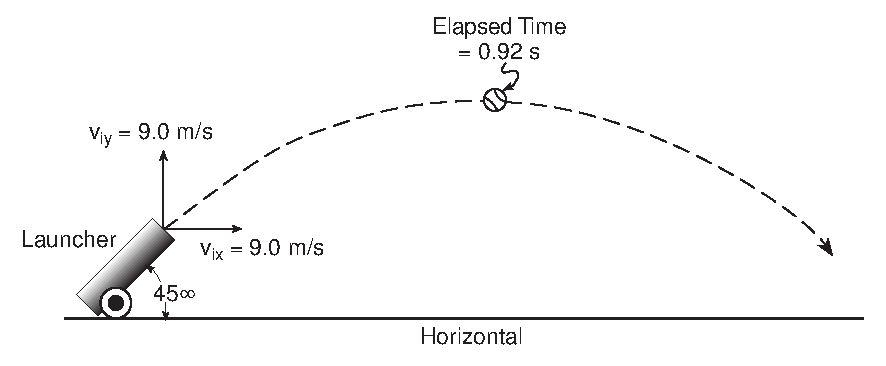
\includegraphics[keepaspectratio,width=\columnwidth]{June2000-Q56}
    \end{center}
    The speed of the tennis ball as it leaves the launcher is approximately:
    \begin{multicols}{2}
    \begin{choices}
        \wrongchoice{\SI{4.5}{\meter\per\second}}
      \correctchoice{\SI{13}{\meter\per\second}}
        \wrongchoice{\SI{8.3}{\meter\per\second}}
        \wrongchoice{\SI{18}{\meter\per\second}}
    \end{choices}
    \end{multicols}
\end{question}
}

\element{nysed}{
\begin{question}{June2000-Q57}
    A machine launches a tennis ball at an angle of \ang{45} with the horizontal,
        as shown.
    The ball has an initial vertical velocity of \SI{9.0}{\meter\per\second} and an initial horizontal velocity of \SI{9.0}{\meter\per\second}.
    The ball reaches its maximum height \SI{0.92}{\second} after its launch.
    [Neglect air resistance and assume the ball lands at the same height above the ground from which it was launched.]
    \begin{center}
        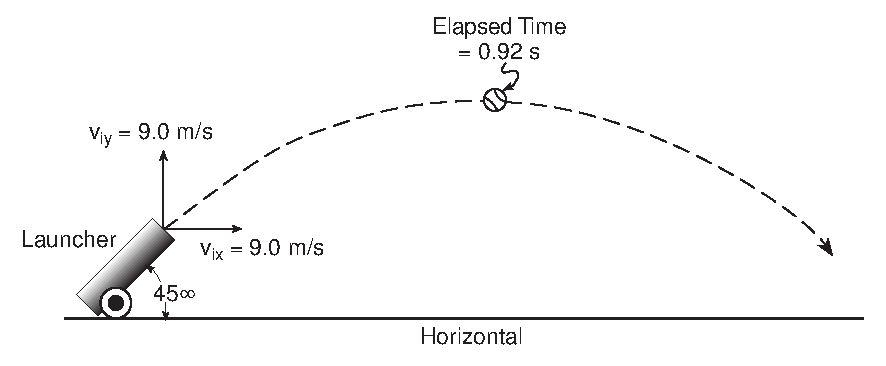
\includegraphics[keepaspectratio,width=\columnwidth]{June2000-Q56}
    \end{center}
    The total horizontal distance traveled by the tennis ball during the entire time it is in the air is approximately:
    \begin{multicols}{2}
    \begin{choices}
        \wrongchoice{\SI{23}{\meter}}
        \wrongchoice{\SI{17}{\meter}}
      \correctchoice{\SI{8.3}{\meter}}
        \wrongchoice{\SI{4.1}{\meter}}
    \end{choices}
    \end{multicols}
\end{question}
}

\element{nysed}{
\begin{question}{June2000-Q58}
    A machine launches a tennis ball at an angle of \ang{45} with the horizontal,
        as shown.
    The ball has an initial vertical velocity of \SI{9.0}{\meter\per\second} and an initial horizontal velocity of \SI{9.0}{\meter\per\second}.
    The ball reaches its maximum height \SI{0.92}{\second} after its launch.
    [Neglect air resistance and assume the ball lands at the same height above the ground from which it was launched.]
    \begin{center}
        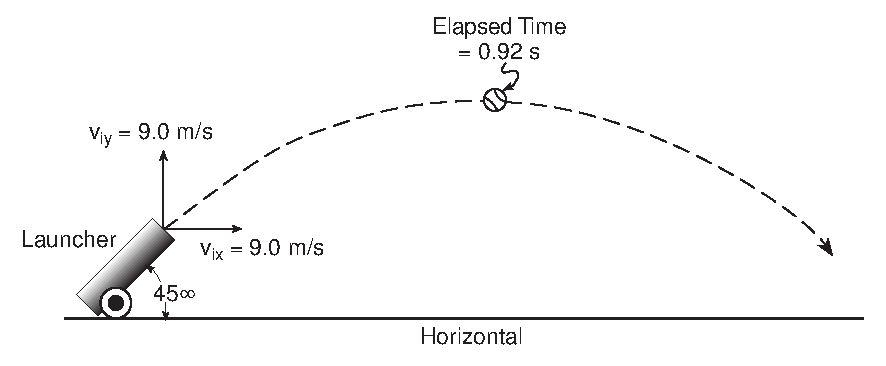
\includegraphics[keepaspectratio,width=\columnwidth]{June2000-Q56}
    \end{center}
    The speed at which the launcher fires tennis balls is constant,
        but the angle between the launcher and the horizontal can be varied.
    As the angle is decreased from \ang{45} to \ang{30},
        the range of the tennis balls:
    \begin{choices}
      \correctchoice{decreases}
        \wrongchoice{increases}
        \wrongchoice{remains the same}
    \end{choices}
\end{question}
}

\element{nysed}{
\begin{question}{June2000-Q59}
    A \SI{2}{\kilo\gram} block is dropped from the roof of a tall building at the same time a \SI{6}{\kilo\gram} ball is thrown horizontally from the same height.
    Which statement best describes the motion of the block and the motion of the ball? [Neglect air resistance]
    \begin{choices}
        \wrongchoice{The \SI{2}{\kilo\gram} block hits the ground first because it has no horizontal velocity.}
        \wrongchoice{The \SI{6}{\kilo\gram} block hits the ground first because it has more mass.}
        \wrongchoice{The \SI{6}{\kilo\gram} block hits the ground first because it is round.}
      \correctchoice{The block and the ball hit the ground at the same time because they have the same vertical acceleration}
    \end{choices}
\end{question}
}


%% Section June1999
%%--------------------
\element{nysed}{
\begin{question}{June1999-Q58}
    The diagram below shows the muzzle of a cannon located \SI{50}{\meter} above the ground.
    When the cannon is fired, a ball leaves the muzzle with an initial speed of \SI{250}{\meter\per\second}.
    [Neglect air resistance]
    \begin{center}
    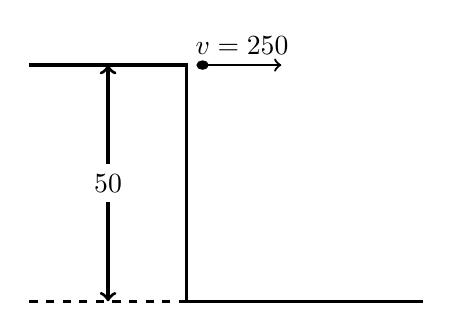
\begin{tikzpicture}[yscale=0.75]
        \draw[very thick] (-2,0) -- (0,0) -- (0,-4) -- (3,-4);
        \draw[fill] (0.2,0.0) circle [radius=2pt];
        \draw[thick,->] (0.2,0.0) -- ++ (0:1)
            node[anchor=south] at ++ (0:-0.5) {$v=\SI{250}{\meter\per\second}$};
        \draw[very thick,dashed] (-2,-4) -- (0,-4);
        \node (A) at (-1,-2.0) {\SI{50}{\meter}};
        \draw[very thick,->] (A) -- (-1,0);
        \draw[very thick,->] (A) -- (-1,-4);
    \end{tikzpicture}
    \end{center}
    Which action would most likely increase the time of flight of the ball fired by the cannon?
    \begin{choices}
        \wrongchoice{pointing the muzzle of the cannon toward the ground}
        \wrongchoice{moving the cannon closer to the edge of the cliff}
      \correctchoice{positioning the cannon higher above the ground}
        \wrongchoice{giving the ball a greater initial horizontal velocity}
    \end{choices}
\end{question}
}

\element{nysed}{
\begin{question}{June1999-Q62}
    In the diagram below,
        a stationary observer on the ground watches as a seagull flying horizontally to the right drops a clamshell.
    \begin{center}
        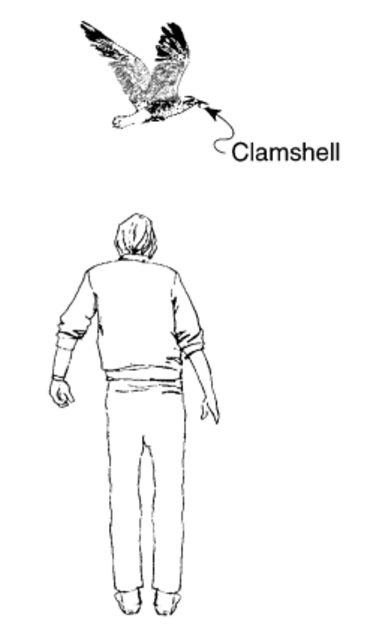
\includegraphics[keepaspectratio,scale=0.66]{June1999-Q62}
    \end{center}
    Which diagram best represents the path of the falling clamshell as seen by the observer?
    [Neglect air resistance]
    \begin{multicols}{2}
    \begin{choices}
        \AMCboxDimensions{down=-0.40cm}
        \wrongchoice{
            \begin{tikzpicture}
                \draw[white] (-0.5,0) rectangle (0.5,-1);
                \draw[thick,->] (0,0) -- (0,-1);
            \end{tikzpicture}
        }
        \wrongchoice{
            \begin{tikzpicture}
                \draw[white] (-0.15,+0.15) rectangle (+0.85,-0.85);
                \draw[thick,->] (0,0) -- (0.707,-0.707);
            \end{tikzpicture}
        }
        \wrongchoice{
            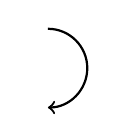
\begin{tikzpicture}
                \draw[white] (-0.25,0) rectangle (0.75,-1);
                \draw[thick,->] (0,0) arc (90:-90:0.50);
            \end{tikzpicture}
        }
        \correctchoice{
            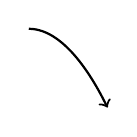
\begin{tikzpicture}
                \draw[white] (0,1) rectangle (1,0);
                \draw[thick,->] (0,1) parabola (1,0);
            \end{tikzpicture}
        }
    \end{choices}
    \end{multicols}
\end{question}
}


%% Section June1998
%%--------------------
\element{nysed}{
\begin{question}{June1998-Q56}
    A student standing on a knoll throws a snowball horizontally \SI{4.5}{\meter} above the level ground towards a smokestack \SI{15}{\meter} away.
    The snowball hits the smokestack \SI{0.65}{\second} after being released. 
    [Neglect air resistance]
    \begin{center}
        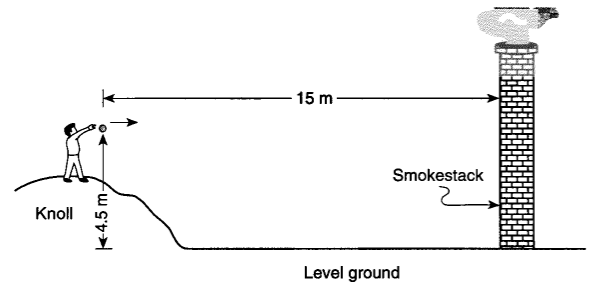
\includegraphics[keepaspectratio,width=\linewidth]{June1998-Q56}
    \end{center}
    Approximately how far above the level ground does the snowball hit the smokestack?
    \begin{multicols}{2}
    \begin{choices}
        \wrongchoice{\SI{0.0}{\meter}}
        \wrongchoice{\SI{0.4}{\meter}}
      \correctchoice{\SI{2.4}{\meter}}
        \wrongchoice{\SI{4.5}{\meter}}
    \end{choices}
    \end{multicols}
\end{question}
}

\element{nysed}{
\begin{question}{June1998-Q57}
    A student standing on a knoll throws a snowball horizontally \SI{4.5}{\meter} above the level ground towards a smokestack \SI{15}{\meter} away.
    The snowball hits the smokestack \SI{0.65}{\second} after being released. 
    [Neglect air resistance]
    \begin{center}
        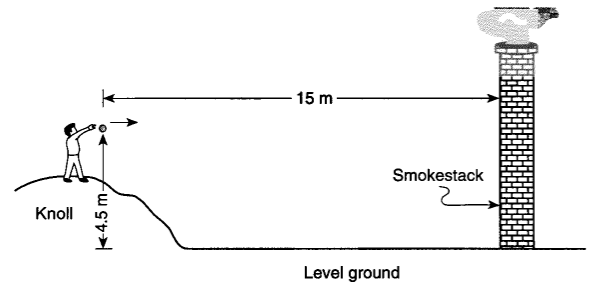
\includegraphics[keepaspectratio,width=0.95\linewidth]{June1998-Q56}
    \end{center}
    At the instant the snowball is released,
        the horizontal component of its velocity is approximately:
    \begin{multicols}{2}
    \begin{choices}
        \wrongchoice{\SI{6.9}{\meter\per\second}}
        \wrongchoice{\SI{9.8}{\meter\per\second}}
        \wrongchoice{\SI{17}{\meter\per\second}}
      \correctchoice{\SI{23}{\meter\per\second}}
    \end{choices}
    \end{multicols}
\end{question}
}

\element{nysed}{
\begin{question}{June1998-Q62}
    The diagram below shows a projectile moving with speed $v$ at the top of its trajectory.
    \begin{center}
    \begin{tikzpicture}
        %% Ground
        \draw[thick] (-3.5,0) -- (3.5,0);
        \node[anchor=north,fill,pattern=north east lines,minimum width=7cm, minimum height=0.05cm] at (0,0) {};
        \node[anchor=north] at (0,-1em) {Ground};
        %% Path: y = 2/9 x^2, y' = 4/9 x, dy/dx (2) = 12/9, atan(12/9) = 53
        \draw[thick,dashed] (-3,0) parabola bend (0,2) (3,0);
        \draw[thick,->] (-3,0) -- ++(53:1);
        %% Projectile
        \draw[fill] (0,2) circle (3pt) node[anchor=north,yshift=-3pt,font=\small] {Projectile};
        \draw[thick,->] (-0.5,2.4) -- (0.5,2.4) node[pos=0.5,anchor=south] {$v$};
    \end{tikzpicture}
    \end{center}
    Which vector best represents the acceleration of the projectile in the position shown?
    \begin{multicols}{4}
    \begin{choices}
        \AMCboxDimensions{down=-0.2cm}
        \correctchoice{
            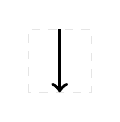
\begin{tikzpicture}[scale=0.4]
                \draw[dashed,white!90!black] (0,0) rectangle (2,2);
                \draw[very thick,->] (1,2) -- (1,0);
            \end{tikzpicture}
        }
        \wrongchoice{
            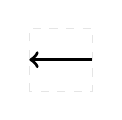
\begin{tikzpicture}[scale=0.4]
                \draw[dashed,white!90!black] (0,0) rectangle (2,2);
                \draw[very thick,->] (2,1) -- (0,1);
            \end{tikzpicture}
        }
        \wrongchoice{
            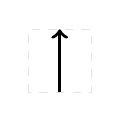
\begin{tikzpicture}[scale=0.4]
                \draw[dashed,white!90!black] (0,0) rectangle (2,2);
                \draw[very thick,->] (1,0) -- (1,2);
            \end{tikzpicture}
        }
        \wrongchoice{
            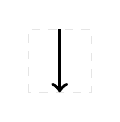
\begin{tikzpicture}[scale=0.4]
                \draw[dashed,white!90!black] (0,0) rectangle (2,2);
                \draw[very thick,->] (1,2) -- (1,0);
            \end{tikzpicture}
        }
    \end{choices}
    \end{multicols}
\end{question}
}


%% Section June1997
%%--------------------
\element{nysed}{
\begin{question}{June1997-Q62}
    Projectiles are fired from different angles with the same speed of \SI{14}{\meter\per\second}.
    The graph below shows the range of the projectiles as a function of the original angle of inclination to the ground, neglecting air resistance.
    \begin{center}
    \begin{tikzpicture}
        \begin{axis}[
            axis y line=left, 
            axis x line=bottom, 
            axis line style={->},
            xlabel={Angle},
            x unit=\si{\degree},
            xtick={0,10,20,30,40,50,60,70,80,90},
            ylabel={Range},
            y unit=\si{\meter},
            ytick={0,5,10,15,20},
            grid=major,
            xmin=0,xmax=90,
            ymin=0,ymax=21,
            width=0.8\columnwidth,
            height=0.5\columnwidth,
        ]
        \addplot[line width=1pt,domain=0:90]{20*sin(2*x)};
        \end{axis}
    \end{tikzpicture}
    \end{center}
    The graph shows that the range of the projectile is:
    \begin{choices}
        \wrongchoice{the same for all angles.}
        \wrongchoice{the same for angles of \ang{20} and \ang{80}.}
      \correctchoice{greatest for an angle of \ang{45}.}
        \wrongchoice{greatest for an angle of \ang{90}.}
    \end{choices}
\end{question}
}

\element{nysed}{
\begin{question}{June1997-Q64}
    Four different balls are thrown horizontally off the top of four cliffs.
    In which diagram does the ball have the shortest time of flight?
    \begin{multicols}{2}
    \begin{choices}
        \AMCboxDimensions{down=-1cm}
        \correctchoice{
            \begin{tikzpicture}[font=\footnotesize]
                \draw[dashed,white!90!black] (-1.5,-1.2em) rectangle (1.5,4.3);
                %% Cliff
                \draw[thick] (-1,1) -- (0,1) -- (0,0) -- (1,0);
                \node[anchor=south,rotate=270] at (0,0.5) {Cliff};
                \node[anchor=north,rotate=0.0] at (0.5,0) {Ground};
                %% Height
                \draw[<->] (-0.9,1) -- (-0.9,0) node[pos=0.5,anchor=center,fill=white] {\SI{125}{\meter}};
                %% Mass
                \draw[fill] (0,1.33) circle (1.5pt) node[anchor=east] {\SI{1.0}{\kilo\gram}};
                %% velocity
                \draw[thick,->] (0,1.33) -- ++ (0:1) node[pos=0.5,anchor=south] {\SI{50}{\meter\per\second}};
            \end{tikzpicture}
        }
        \wrongchoice{
            \begin{tikzpicture}[font=\footnotesize]
                \draw[dashed,white!90!black] (-1.5,-1.2em) rectangle (1.5,4.3);
                %% Cliff
                \draw[thick] (-1,2) -- (0,2) -- (0,0) -- (1,0);
                \node[anchor=south,rotate=270] at (0,1.0) {Cliff};
                \node[anchor=north,rotate=0.0] at (0.5,0) {Ground};
                %% Height
                \draw[<->] (-0.9,2) -- (-0.9,0) node[pos=0.5,anchor=center,fill=white] {\SI{250}{\meter}};
                %% Mass
                \draw[fill] (0,2.33) circle (1.5pt) node[anchor=east] {\SI{0.5}{\kilo\gram}};
                %% velocity
                \draw[thick,->] (0,2.33) -- ++ (0:1) node[pos=0.5,anchor=south] {\SI{40}{\meter\per\second}};
            \end{tikzpicture}
        }
        \wrongchoice{
            \begin{tikzpicture}[font=\footnotesize]
                \draw[dashed,white!90!black] (-1.5,-1.2em) rectangle (1.5,4.3);
                %% Cliff
                \draw[thick] (-1,3) -- (0,3) -- (0,0) -- (1,0);
                \node[anchor=south,rotate=270] at (0,1.5) {Cliff};
                \node[anchor=north,rotate=0.0] at (0.5,0) {Ground};
                %% Height
                \draw[<->] (-0.9,3) -- (-0.9,0) node[pos=0.5,anchor=center,fill=white] {\SI{375}{\meter}};
                %% Mass
                \draw[fill] (0,3.33) circle (1.5pt) node[anchor=east] {\SI{0.25}{\kilo\gram}};
                %% velocity
                \draw[thick,->] (0,3.33) -- ++ (0:1) node[pos=0.5,anchor=south] {\SI{35}{\meter\per\second}};
            \end{tikzpicture}
        }
        \wrongchoice{
            \begin{tikzpicture}[font=\footnotesize]
                \draw[dashed,white!90!black] (-1.5,-1.2em) rectangle (1.5,4.3);
                %% Cliff
                \draw[thick] (-1,3.6) -- (0,3.6) -- (0,0) -- (1,0);
                \node[anchor=south,rotate=270] at (0,1.5) {Cliff};
                \node[anchor=north,rotate=0.0] at (0.5,0) {Ground};
                %% Height
                \draw[<->] (-0.9,3.6) -- (-0.9,0) node[pos=0.5,anchor=center,fill=white] {\SI{450}{\meter}};
                %% Mass
                \draw[fill] (0,3.9) circle (1.5pt) node[anchor=east] {\SI{0.1}{\kilo\gram}};
                %% velocity
                \draw[thick,->] (0,3.9) -- ++ (0:1) node[pos=0.5,anchor=south] {\SI{35}{\meter\per\second}};
            \end{tikzpicture}
        }
    \end{choices}
    \end{multicols}
\end{question}
}


%% Section June1996
%%--------------------
\newcommand{\JuneNineteenNinetySixQFiftySix}{
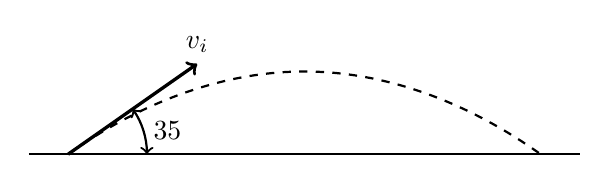
\begin{tikzpicture}
    %% NOTE: useful reference
    %% \frac{h}{R} = \frac{\tan\theta}{4}
    \draw[thick] (-3.5,0) -- (3.5,0);
    \draw[thick,dashed] (-3,0) parabola bend (0,1.05) (3,0);
    \draw[very thick,->] (-3,0) -- ++ (35:2.0cm) node[pos=1.0,anchor=south] {$v_i$};
    \draw[thick,<->] (-2,0) arc (0:35:1cm) node[pos=0.5,anchor=west] {\ang{35}};
\end{tikzpicture}
}

\element{nysed}{
\begin{question}{June1996-Q56}
    A cannon elevated at an angle of \ang{35} to the horizontal fires a cannonball,
        which travels the path shown in the diagram below.
    [Neglect air resistance and assume the ball lands at the same height above the ground from which it was launched.]
    \begin{center}
        \JuneNineteenNinetySixQFiftySix
    \end{center}
    If the ball lands \SI{7.0e2}{\meter} from the cannon \SI{10}{\second} after it was fired,
        what is the horizontal component of its initial velocity?
    \begin{multicols}{2}
    \begin{choices}
      \correctchoice{\SI{70}{\meter\per\second}}
        \wrongchoice{\SI{49}{\meter\per\second}}
        \wrongchoice{\SI{35}{\meter\per\second}}
        \wrongchoice{\SI{7.0}{\meter\per\second}}
    \end{choices}
    \end{multicols}
\end{question}
}

\element{nysed}{
\begin{question}{June1996-Q57}
    A cannon elevated at an angle of \ang{35} to the horizontal fires a cannonball,
        which travels the path shown in the diagram below.
    [Neglect air resistance and assume the ball lands at the same height above the ground from which it was launched.]
    \begin{center}
        \JuneNineteenNinetySixQFiftySix
    \end{center}
    If the ball's time of flight is \SI{10}{\second},
        what is the vertical component of its initial velocity?
    \begin{multicols}{2}
    \begin{choices}
        \wrongchoice{\SI{9.8}{\meter\per\second}}
      \correctchoice{\SI{49}{\meter\per\second}}
        \wrongchoice{\SI{70}{\meter\per\second}}
        \wrongchoice{\SI{98}{\meter\per\second}}
    \end{choices}
    \end{multicols}
\end{question}
}

\element{nysed}{
\begin{question}{June1996-Q58}
    A cannon elevated at an angle of \ang{35} to the horizontal fires a cannonball,
        which travels the path shown in the diagram below.
    [Neglect air resistance and assume the ball lands at the same height above the ground from which it was launched.]
    \begin{center}
        \JuneNineteenNinetySixQFiftySix
    \end{center}
    If the angle of elevation of the cannon is decreased from \ang{35} to \ang{30},
        the vertical component of the ball's initial velocity will:
    \begin{choices}
        \wrongchoice{decrease and its horizontal will decrease.}
      \correctchoice{decrease and its horizontal will increase.}
        \wrongchoice{increase and its horizontal will decrease.}
        \wrongchoice{increase and its horizontal will increase.}
    \end{choices}
\end{question}
}

\element{nysed}{
\begin{question}{June1996-Q65}
    A ball is projected horizontally to the right from a height of \SI{50}{\meter},
        as shown in the diagram below.
    \begin{center}
    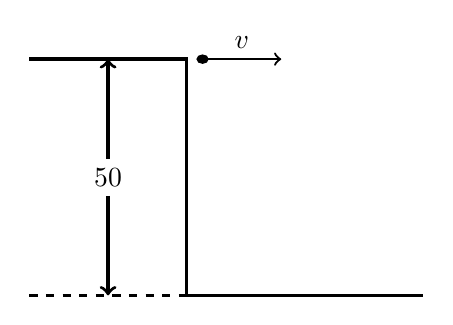
\begin{tikzpicture}[yscale=0.75]
        \draw[very thick] (-2,0) -- (0,0) -- (0,-4) -- (3,-4);
        \draw[fill] (0.2,0.0) circle [radius=2pt];
        \draw[thick,->] (0.2,0.0) -- ++ (0:1)
            node[anchor=south] at ++ (0:-0.5) {$v$};
        \draw[very thick,dashed] (-2,-4) -- (0,-4);
        \node (A) at (-1,-2.0) {\SI{50}{\meter}};
        \draw[very thick,->] (A) -- (-1,0);
        \draw[very thick,->] (A) -- (-1,-4);
    \end{tikzpicture}
    \end{center}
    Which diagram best represents the position of the ball at \SI{1.0}{\second} intervals?
    [Neglect air resistance.]
    \begin{multicols}{2}
    \begin{choices}
        \AMCboxDimensions{down=-1.5em}
        \correctchoice{
            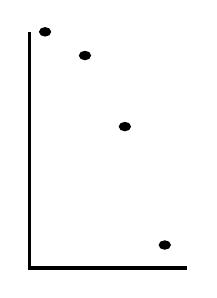
\begin{tikzpicture}[yscale=0.75]
                \draw[very thick] (0,0) -- (0,-4) -- (2,-4);
                \draw[domain=0:3.8,samples=4,mark=*,only marks] plot ({0.2+0.4*\x}, {-0.25*\x*\x});
            \end{tikzpicture}
        }
        \wrongchoice{
            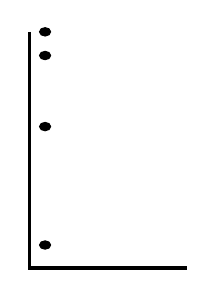
\begin{tikzpicture}[yscale=0.75]
                \draw[very thick] (0,0) -- (0,-4) -- (2,-4);
                \draw[domain=0:3.8,samples=4,mark=*,only marks] plot (0.2, {-0.25*\x*\x});
            \end{tikzpicture}
        }
        \wrongchoice{
            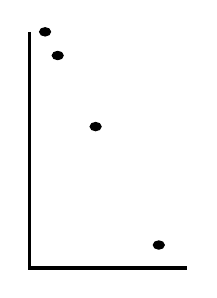
\begin{tikzpicture}[yscale=0.75]
                \draw[very thick] (0,0) -- (0,-4) -- (2,-4);
                \draw[domain=0:3.8,samples=4,mark=*,only marks] plot ({0.2+0.10*\x*\x}, {-0.25*\x*\x});
            \end{tikzpicture}
        }
        \wrongchoice{
            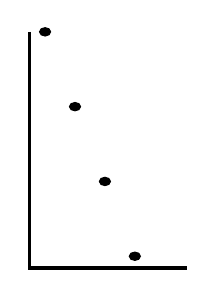
\begin{tikzpicture}[yscale=0.75]
                \draw[very thick] (0,0) -- (0,-4) -- (2,-4);
                \draw[domain=0:3.8,samples=4,mark=*,only marks] plot ({0.2+0.3*\x}, {-1.0*\x});
            \end{tikzpicture}
        }
    \end{choices}
    \end{multicols}
\end{question}
}

\endinput



%
%% Newton Questions used on the
%% NYSED Physics Regents Examination
%%--------------------------------------------------

%% this section contains 105 problems


%% Section June2015
%%--------------------
\element{nysed}{
\begin{question}{June2015-Q04}
    A \SI{160}{\kilo\gram} space vehicle is traveling along a straight line at a constant speed of \SI{800}{\meter\per\second}. 
    The magnitude of the net force on the space vehicle is:
    \begin{multicols}{2}
    \begin{choices}
      \correctchoice{\SI{0}{\newton}}
        \wrongchoice{\SI{1.60e2}{\newton}}
        \wrongchoice{\SI{8.00e2}{\newton}}
        \wrongchoice{\SI{1.28e5}{\newton}}
    \end{choices}
    \end{multicols}
\end{question}
}

\element{nysed}{
\begin{question}{June2015-Q05}
    A student throws a \SI{5.0}{\newton} ball straight up.
    What is the net force on the ball at its maximum height?
    \begin{multicols}{2}
    \begin{choices}
        \wrongchoice{\SI{0.0}{\newton}}
        \wrongchoice{\SI{5.0}{\newton}, up}
      \correctchoice{\SI{5.0}{\newton}, down}
        \wrongchoice{\SI{9.8}{\newton}, down}
    \end{choices}
    \end{multicols}
\end{question}
}

\element{nysed}{
\begin{question}{June2015-Q07}
    A \SI{1.5}{\kilo\gram} cart initially moves at \SI{2.0}{\meter\per\second}.
    It is brought to rest by a constant net force in \SI{0.30}{\second}.
    What is the magnitude of the net force?
    \begin{multicols}{2}
    \begin{choices}
        \wrongchoice{\SI{0.40}{\newton}}
        \wrongchoice{\SI{0.90}{\newton}}
      \correctchoice{\SI{10}{\newton}}
        \wrongchoice{\SI{15}{\newton}}
    \end{choices}
    \end{multicols}
\end{question}
}

\element{nysed}{
\begin{question}{June2015-Q09}
    As a \SI{5.0e2}{\newton} basketball player jumps from the floor up toward the basket,
        the magnitude of the force of her feet on the floor is \SI{1.0e3}{\newton}.
    As she jumps, the magnitude of the force of the floor on her feet is:
    \begin{multicols}{2}
    \begin{choices}
        \wrongchoice{\SI{5.0e2}{\newton}}
      \correctchoice{\SI{1.0e3}{\newton}}
        \wrongchoice{\SI{1.5e3}{\newton}}
        \wrongchoice{\SI{5.0e5}{\newton}}
    \end{choices}
    \end{multicols}
\end{question}
}

\element{nysed}{
\begin{question}{June2015-Q33}
    A different force is applied to each of four different blocks on a frictionless, horizontal surface. 
    In which diagram does the block have the greatest inertia \SI{2.0}{\second} after starting from rest?
    \begin{multicols}{2}
    \begin{choices}
        \AMCboxDimensions{down=-0.20cm}
        \correctchoice{
            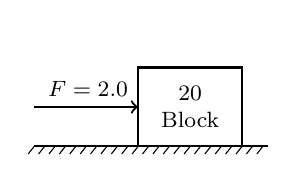
\begin{tikzpicture}[font=\footnotesize,xscale=0.66]
                \draw[white] (-2.0,1.5) -- (2.0,1.5);
                %% Force
                \draw[thick,->] (-2,0.5) -- (0,0.5)
                    node[pos=1.0,anchor=south east] {$F=\SI{2.0}{\newton}$};
                %% Block
                \draw[thick] (0,0) rectangle (2,1);
                \node[anchor=center,text width=3em,text centered]
                    at (1,0.5) {\SI{20}{\kilo\gram} Block};
                %% Floor
                \draw[thick] (-2,0) -- (2.5,0);
                \foreach \x in {-20,-18,...,25}
                    \draw[thin] (\x mm,0cm) -- ++ (220:0.15cm);
            \end{tikzpicture}
        }
        \wrongchoice{
            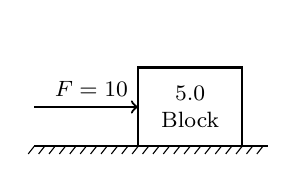
\begin{tikzpicture}[font=\footnotesize,xscale=0.66]
                \draw[white] (-2.0,1.5) -- (2.0,1.5);
                %% Force
                \draw[thick,->] (-2,0.5) -- (0,0.5)
                    node[pos=1.0,anchor=south east] {$F=\SI{10}{\newton}$};
                %% Block
                \draw[thick] (0,0) rectangle (2,1);
                \node[anchor=center,text width=3em,text centered]
                    at (1,0.5) {\SI{5.0}{\kilo\gram} Block};
                %% Floor
                \draw[thick] (-2,0) -- (2.5,0);
                \foreach \x in {-20,-18,...,25}
                    \draw[thin] (\x mm,0cm) -- ++ (220:0.15cm);
            \end{tikzpicture}
        }
        \wrongchoice{
            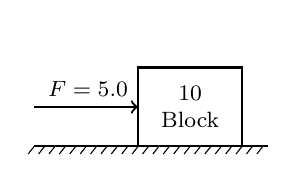
\begin{tikzpicture}[font=\footnotesize,xscale=0.66]
                \draw[white] (-2.0,1.5) -- (2.0,1.5);
                %% Force
                \draw[thick,->] (-2,0.5) -- (0,0.5)
                    node[pos=1.0,anchor=south east] {$F=\SI{5.0}{\newton}$};
                %% Block
                \draw[thick] (0,0) rectangle (2,1);
                \draw[thick] (0,0) rectangle (2,1);
                \node[anchor=center,text width=3em,text centered]
                    at (1,0.5) {\SI{10}{\kilo\gram} Block};
                %% Floor
                \draw[thick] (-2,0) -- (2.5,0);
                \foreach \x in {-20,-18,...,25}
                    \draw[thin] (\x mm,0cm) -- ++ (220:0.15cm);
            \end{tikzpicture}
        }
        \wrongchoice{
            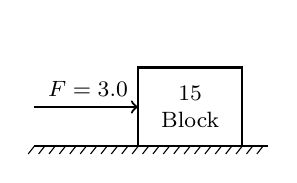
\begin{tikzpicture}[font=\footnotesize,xscale=0.66]
                \draw[white] (-2.0,1.5) -- (2.0,1.5);
                %% Force
                \draw[thick,->] (-2,0.5) -- (0,0.5)
                    node[pos=1.0,anchor=south east] {$F=\SI{3.0}{\newton}$};
                %% Block
                \draw[thick] (0,0) rectangle (2,1);
                \node[anchor=center,text width=3em,text centered]
                    at (1,0.5) {\SI{15}{\kilo\gram} Block};
                %% Floor
                \draw[thick] (-2,0) -- (2.5,0);
                \foreach \x in {-20,-18,...,25}
                    \draw[thin] (\x mm,0cm) -- ++ (220:0.15cm);
            \end{tikzpicture}
        }
    \end{choices}
    \end{multicols}
\end{question}
}

\element{nysed}{
\begin{question}{June2015-Q41}
    An object is in equilibrium. 
    Which force vector diagram could represent the force(s) acting on the object?
    \begin{multicols}{2}
    \begin{choices}
        \AMCboxDimensions{down=-1.3cm}
        \wrongchoice{
            \begin{tikzpicture}
                \draw[white] (-1.00,-1.5) rectangle (1.00,1.0);
                \node[draw,fill=white!90!black,circle,inner sep=0pt,minimum size=8pt] (A) at (0,0) {};
                \draw[thick,->] (A) -- ++ (270:1.414cm);
            \end{tikzpicture}
        }
        \wrongchoice{
            \begin{tikzpicture}
                \draw[white] (-1.00,-1.5) rectangle (1.00,1.0);
                \node[draw,fill=white!90!black,circle,inner sep=0pt,minimum size=8pt] (A) at (0,0) {};
                \draw[thick,->] (A) -- ++ (270:1.414cm);
                \draw[thick,->] (A) -- ++ (90:0.707cm);
            \end{tikzpicture}
        }
        \wrongchoice{
            \begin{tikzpicture}
                \draw[white] (-1.00,-1.5) rectangle (1.00,1.0);
                \node[draw,fill=white!90!black,circle,inner sep=0pt,minimum size=8pt] (A) at (0,0) {};
                \draw[thick,->] (A) -- ++ (0:0.707cm);
                \draw[thick,->] (A) -- ++ (180:0.707cm);
                \draw[thick,->] (A) -- ++ (270:1.414cm);
            \end{tikzpicture}
        }
        \correctchoice{
            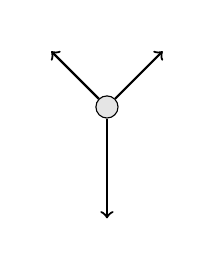
\begin{tikzpicture}
                \draw[white] (-1.00,-1.5) rectangle (1.00,1.0);
                \node[draw,fill=white!90!black,circle,inner sep=0pt,minimum size=8pt] (A) at (0,0) {};
                \draw[thick,->] (A) -- ++ (45:1.00cm);
                \draw[thick,->] (A) -- ++ (135:1.00cm);
                \draw[thick,->] (A) -- ++ (270:1.414cm);
            \end{tikzpicture}
        }
    \end{choices}
    \end{multicols}
\end{question}
}


%% Section June2014
%%--------------------
\element{nysed}{
\begin{question}{June2014-Q05}
    A baseball bat exerts a force of magnitude $F$ on a ball.
    If the mass of the bat is three times the mass of the ball,
        the magnitude of the force of the ball on the bat is:
    \begin{multicols}{2}
    \begin{choices}
      \correctchoice{$F$}
        \wrongchoice{$2F$}
        \wrongchoice{$3F$}
        \wrongchoice{$F/3$}
    \end{choices}
    \end{multicols}
\end{question}
}

\element{nysed}{
\begin{question}{June2014-Q08}
    A \SI{750}{\newton} person stands in an elevator that is accelerating downward.
    The upward force of the elevator floor on the person must be:
    \begin{choices}
      \correctchoice{less than \SI{750}{\newton}}
        \wrongchoice{equal to \SI{0}{\newton}}
        \wrongchoice{equal to \SI{750}{\newton}}
        \wrongchoice{greater than \SI{750}{\newton}}
    \end{choices}
\end{question}
}


%% Section June2013
%%--------------------
\element{nysed}{
\begin{question}{June2013-Q09}
    Which situation represents a person in equilibrium?
    \begin{choices}
        \wrongchoice{a child gaining speed while sliding a slide}
        \wrongchoice{a woman accelerating upward in an elevator}
      \correctchoice{a man standing on a bathroom scale}
        \wrongchoice{a teenager driving around a corner in his car}
    \end{choices}
\end{question}
}

\element{nysed}{
\begin{question}{June2013-Q10}
    A rock is thrown straight up into the air.
    At the highest point of the rock's path,
        the magnitude of the net force acting on the rock is:
    \begin{choices}
        \wrongchoice{less than the magnitude of the rock's weight, but greater than zero}
        \wrongchoice{greater than the magnitude of the rock's weight}
      \correctchoice{the same as the magnitude of the rock's weight}
        \wrongchoice{zero}
    \end{choices}
\end{question}
}

\element{nysed}{
\begin{question}{June2013-Q11}
    The diagram below shows a compressed spring between two carts initially at rest on a horizontal frictionless surface.
    Cart $A$ has a mass of \SI{2.0}{\kilo\gram} and cart $B$ has a mass of \SI{1.0}{\kilo\gram}.
    A string holds the carts together.
    \begin{center}
    \begin{tikzpicture}
        %% Ground
        \node[anchor=north,fill,pattern=north east lines,minimum width=8cm, minimum height=0.05cm] at (0,0) {};
        \draw (-4,0) -- (4,0);
        %% carts
        \node[draw,minimum width=2cm,minimum height=2em,anchor=south] (A) at (-2,0.3) {\SI{2}{\kilo\gram}};
        \node[draw,minimum width=1cm,minimum height=2em,anchor=south] (B) at (2,0.3) {\SI{1}{\kilo\gram}};
        \node[anchor=south] at (A.north) {$A$};
        \node[anchor=south] at (B.north) {$B$};
        %% wheels
        \draw[fill=white!90!black] (A.south west) ++(0:0.2cm) arc(90:-270:0.15);
        \draw[fill=white!90!black] (A.south east) ++(180:0.2cm) arc(90:-270:0.15);
        \draw[fill=white!90!black] (B.south west) ++(0:0.2cm) arc(90:-270:0.15);
        \draw[fill=white!90!black] (B.south east) ++(180:0.2cm) arc(90:-270:0.15);
        %% Spring
        \draw[decoration={aspect=0.2,segment length=1.5mm,amplitude=2mm,coil},decorate] (A.east) -- (B.west);
        \draw[thick] (A.north east) -- (B.north west);
    \end{tikzpicture}
    \end{center}
    The string is cut and the carts move apart.
    Compared to the magnitude of the force the spring exerts on cart $A$,
        the magnitude of the force the spring exerts on cart $B$ is:
    \begin{choices}
      \correctchoice{the same}
        \wrongchoice{half as great}
        \wrongchoice{twice as great}
        \wrongchoice{four times as great}
    \end{choices}
\end{question}
}

\element{nysed}{
\begin{question}{June2013-Q38}
    Four forces act concurrently on a block on a horizontal surface as shown in the diagram below.
    \begin{center}
    \begin{tikzpicture}
        \draw[fill] (0,0) circle (3pt);
        \draw[thick,->] (0,0) -- (0:2cm)
            node[anchor=south] {\SI{100}{\newton}};
        \draw[thick,->] (0,0) -- (90:1.6cm)
            node[anchor=east] {\SI{80}{\newton}};
        \draw[thick,->] (0,0) -- (180:2.4cm)
            node[anchor=south] {\SI{120}{\newton}};
        \draw[thick,->] (0,0) -- (270:1.6cm)
            node[anchor=east] {\SI{80}{\newton}};
        \draw[thick] (-1,-1) rectangle (1,1)
            node[anchor=south] {Block};
        \draw[thick] (-3,-1) -- (3,-1);
        \foreach \x in {-30,-29,...,30}
            \draw[thin] (\x mm,-1cm) -- ++ (220:0.15cm);
    \end{tikzpicture}
    \end{center}
    As a result of these forces, the block:
    \begin{choices}
        \wrongchoice{moves at constant speed to the right}
        \wrongchoice{moves at constant speed to the left}
        \wrongchoice{accelerates to the right}
      \correctchoice{accelerates to the left}
    \end{choices}
\end{question}
}

\element{nysed}{
\begin{question}{June2013-Q40}
    A \SI{4.0}{\kilo\gram} object is accelerated at \SI{3.0}{\meter\per\second\squared} north by an unbalanced force.
    The same unbalanced force acting on a \SI{2.0}{\kilo\gram} object will accelerate this object toward the north at:
    \begin{multicols}{2}
    \begin{choices}
        \wrongchoice{\SI{12}{\meter\per\second\squared}}
      \correctchoice{\SI{6.0}{\meter\per\second\squared}}
        \wrongchoice{\SI{3.0}{\meter\per\second\squared}}
        \wrongchoice{\SI{1.5}{\meter\per\second\squared}}
    \end{choices}
    \end{multicols}
\end{question}
}


%% Section June2012
%%--------------------
\element{nysed}{
\begin{question}{June2012-Q07}
    Which situation describes an object that has \emph{no} unbalanced force acting on it?
    \begin{choices}
        \wrongchoice{an apple in free fall}
        \wrongchoice{a satellite orbiting Earth}
      \correctchoice{a hockey puck moving at constant velocity}
        \wrongchoice{a laboratory cart moving down a frictionless \ang{30} incline}
    \end{choices}
\end{question}
}

\element{nysed}{
\begin{question}{June2012-Q12}
    A number of \SI{1.0}{\newton} horizontal forces are exerted on a block on a frictionless, horizontal surface.
    Which top-view diagram shows the forces producing the greatest magnitude of acceleration of the block?
    \begin{multicols}{2}
    \begin{choices}
        \AMCboxDimensions{down=-1.0cm}
        \correctchoice{
            \begin{tikzpicture}[font=\footnotesize]
                \draw[white] (-1.6,-1.6) rectangle (1.6,1.6);
                \node[draw,rectangle,minimum size=1cm,text centered,text width=1cm]
                    (B) at (0,0) {Top of Block};
                \draw[thick,->] (B.east) -- ++(0:1cm)
                    node[pos=0.5,anchor=south] {\SI{1.0}{\newton}};
                \draw[thick,->] (B.south) -- ++(270:1cm)
                    node[pos=0.5,anchor=east] {\SI{1.0}{\newton}};
            \end{tikzpicture}
        }
        \wrongchoice{
            \begin{tikzpicture}[font=\footnotesize]
                \draw[white] (-1.6,-1.6) rectangle (1.6,1.6);
                \node[draw,rectangle,minimum size=1cm,text centered,text width=1cm]
                    (B) at (0,0) {Top of Block};
                \draw[thick,->] (B.north) -- ++(90:1cm)
                    node[pos=0.5,anchor=east] {\SI{1.0}{\newton}};
                \draw[thick,->] (B.east) -- ++(0:1cm)
                    node[pos=0.5,anchor=south] {\SI{1.0}{\newton}};
                \draw[thick,->] (B.south) -- ++(270:1cm)
                    node[pos=0.5,anchor=east] {\SI{1.0}{\newton}};
                \draw[thick,->] (B.west) -- ++(180:1cm)
                    node[pos=0.5,anchor=south] {\SI{1.0}{\newton}};
            \end{tikzpicture}
        }
        \wrongchoice{
            \begin{tikzpicture}[font=\footnotesize]
                \draw[white] (-1.6,-1.6) rectangle (1.6,1.6);
                \node[draw,rectangle,minimum size=1cm,text centered,text width=1cm]
                    (B) at (0,0) {Top of Block};
                \draw[thick,->] (B.north) -- ++(90:1cm)
                    node[pos=0.5,anchor=east] {\SI{1.0}{\newton}};
                \draw[thick,->] (B.east) -- ++(0:1cm)
                    node[pos=0.5,anchor=south] {\SI{1.0}{\newton}};
                \draw[thick,->] (B.south) -- ++(270:1cm)
                    node[pos=0.5,anchor=east] {\SI{1.0}{\newton}};
            \end{tikzpicture}
        }
        \wrongchoice{
            \begin{tikzpicture}[font=\footnotesize]
                \draw[white] (-1.6,-1.6) rectangle (1.6,1.6);
                \node[draw,rectangle,minimum size=1cm,text centered,text width=1cm]
                    (B) at (0,0) {Top of Block};
                \draw[thick,->] (B.north) -- ++(90:1cm)
                    node[pos=0.5,anchor=east] {\SI{1.0}{\newton}};
                \draw[thick,->] (B.south) -- ++(270:1cm)
                    node[pos=0.5,anchor=east] {\SI{1.0}{\newton}};
            \end{tikzpicture}
        }
    \end{choices}
    \end{multicols}
\end{question}
}

%% NOTE: June2012-Q47 is too big


%% Section June2011
%%--------------------
\element{nysed}{
\begin{question}{June2011-Q06}
    A student is standing in an elevator that is accelerating downward.
    The force that the student exerts on the floor of the elevator must be:
    \begin{choices}
      \correctchoice{less than the weight of the student when at rest}
        \wrongchoice{greater than the weight of the student when at rest}
        \wrongchoice{less than the force of the floor on the student}
        \wrongchoice{greater than the force of the floor on the student}
    \end{choices}
\end{question}
}

\element{nysed}{
\begin{question}{June2011-Q12}
    Two forces act concurrently on an object on a horizontal,
        frictionless surface, as shown in the diagram below.
    \begin{center}
    \begin{tikzpicture}
        %% Ground
        \node[anchor=north,fill,pattern=north east lines,minimum width=8cm, minimum height=0.05cm] at (0,0) {};
        \draw (-4,0) -- (4,0);
        \node at (0,-0.5) {Horizontal, frictionless surface.};
        %% Object
        \node[draw,minimum size=1.6cm,anchor=south] (A) at (0,0) {Object};
        %% Forces
        \draw[thick,->] (A.west) -- ++(180:2) node[pos=0.5,anchor=south] {\SI{10}{\newton}};
        \draw[thick,->] (A.east) -- ++(0:1.2) node[pos=0.5,anchor=south] {\SI{6}{\newton}};
    \end{tikzpicture}
    \end{center}
    What additional force, when applied to the object,
        will establish equilibrium?
    \begin{choices}
        \wrongchoice{\SI{16}{\newton} toward the right}
        \wrongchoice{\SI{16}{\newton} toward the left}
        \wrongchoice{\SI{4}{\newton} toward the right}
      \correctchoice{\SI{4}{\newton} toward the left}
    \end{choices}
\end{question}
}

\element{nysed}{
\begin{question}{June2011-Q38}
    A \SI{75}{\kilo\gram} hockey player is skating across the ice at a speed of \SI{6.0}{\meter\per\second}.
    What is the magnitude of the average force required to stop the player in \SI{0.65}{\second}?
    \begin{multicols}{2}
    \begin{choices}
        \wrongchoice{\SI{120}{\newton}}
        \wrongchoice{\SI{290}{\newton}}
      \correctchoice{\SI{690}{\newton}}
        \wrongchoice{\SI{920}{\newton}}
    \end{choices}
    \end{multicols}
\end{question}
}


%% Section June2010
%%--------------------
\element{nysed}{
\begin{question}{June2010-Q04}
    A \SI{0.149}{\kilo\gram} baseball,
        initially moving at \SI{15}{\meter\per\second},
        is brought to rest in \SI{0.040}{\second} by a baseball glove on a catcher's hand.
    The magnitude of the average force exerted on the ball by the glove is:
    \begin{multicols}{2}
    \begin{choices}
        \wrongchoice{\SI{2.2}{\newton}}
        \wrongchoice{\SI{2.9}{\newton}}
        \wrongchoice{\SI{17}{\newton}}
      \correctchoice{\SI{56}{\newton}}
    \end{choices}
    \end{multicols}
\end{question}
}

\element{nysed}{
\begin{question}{June2010-Q05}
    Which body is in equilibrium?
    \begin{choices}
        \wrongchoice{A satellite moving around Earth in a circular orbit.}
        \wrongchoice{A cart rolling down a frictionless incline.}
        \wrongchoice{An apple falling freely toward the surface of Earth.}
      \correctchoice{A block sliding at constant velocity across a tabletop.}
    \end{choices}
\end{question}
}

\element{nysed}{
\begin{question}{June2010-Q08}
    A student pulls a \SI{60}{\newton} sled with a force having a magnitude of \SI{20}{\newton}.
    What is the magnitude of the force that the sled exerts on the student?
    \begin{multicols}{2}
    \begin{choices}
      \correctchoice{\SI{20}{\newton}}
        \wrongchoice{\SI{40}{\newton}}
        \wrongchoice{\SI{60}{\newton}}
        \wrongchoice{\SI{80}{\newton}}
    \end{choices}
    \end{multicols}
\end{question}
}

\element{nysed}{
\begin{question}{June2010-Q10}
    The diagram below shows a horizontal \SI{12}{\newton} force being applied to two blocks, $A$ and $B$, initially at rest on a horizontal, frictionless surface.
    Block $A$ has a mass of \SI{1.0}{\kilo\gram} and block $B$ has a mass of \SI{2.0}{\kilo\gram}.
    \begin{center}
    \begin{tikzpicture}[font=\footnotesize]
        %% Force
        \draw[thick,->] (-2,0.5) -- (0,0.5)
            node[above left] {$F=\SI{12}{\newton}$};
        %% Block A
        \draw[thick] (0,0) rectangle (1,1);
        \node[anchor=south] at (0.5,0.5) {$A$};
        \node[anchor=north] at (0.5,0.5) {\SI{1.0}{\kilo\gram}};
        %% Block B
        \draw[thick] (1,0) rectangle (2,2);
        \node[anchor=south] at (1.5,1) {$B$};
        \node[anchor=north] at (1.5,1) {\SI{2.0}{\kilo\gram}};
        %% Floor
        \draw[thick] (-3,0) -- (3,0);
        \foreach \x in {-30,-29,...,30}
            \draw[thin] (\x mm,0cm) -- ++ (220:0.15cm);
        \node[anchor=north] at (0,-0.15) {Frictionless surface};
    \end{tikzpicture}
    \end{center}
    The magnitude of the acceleration of block $B$ is:
    \begin{multicols}{2}
    \begin{choices}
        \wrongchoice{\SI{6.0}{\meter\per\second\squared}}
        \wrongchoice{\SI{2.0}{\meter\per\second\squared}}
        \wrongchoice{\SI{3.0}{\meter\per\second\squared}}
      \correctchoice{\SI{4.0}{\meter\per\second\squared}}
    \end{choices}
    \end{multicols}
\end{question}
}


%% Section June2009
%%--------------------
\element{nysed}{
\begin{question}{June2009-Q05}
    A \SI{25}{\newton} weight falls freely from rest from the roof of a building.
    What is the total distance the weight falls in the first \SI{1.0}{\second}?
    \begin{multicols}{2}
    \begin{choices}
        \wrongchoice{\SI{19.6}{\meter}}
        \wrongchoice{\SI{9.8}{\meter}}
      \correctchoice{\SI{4.9}{\meter}}
        \wrongchoice{\SI{2.5}{\meter}}
    \end{choices}
    \end{multicols}
\end{question}
}

\element{nysed}{
\begin{question}{June2009-Q09}
    A \SI{0.50}{\kilo\gram} cart is rolling at a speed of \SI{0.40}{\meter\per\second}.
    If the speed of the cart is doubled, the inertia of the cart is:
    \begin{multicols}{2}
    \begin{choices}
        \wrongchoice{halved}
        \wrongchoice{doubled}
        \wrongchoice{quadrupled}
      \correctchoice{unchanged}
    \end{choices}
    \end{multicols}
\end{question}
}

\element{nysed}{
\begin{question}{June2009-Q10}
    Two forces, $F_1$ and $F_2$, are applied to a block on a frictionless,
        horizontal surface as shown below.
    \begin{center}
    \begin{tikzpicture}[xscale=0.95]
        %% Force 1
        \draw[thick,->] (0,0.5) -- (-4,0.5)
            node[above right] {$F_1=\SI{12}{\newton}$};
        %% Force 2
        \draw[thick,->] (2,0.5) -- (2.667,0.5);
        \node[anchor=south west] at (2,0.5) {$F_2=\SI{2}{\newton}$};
        %% Block
        \draw[thick] (0,0) rectangle (2,1);
        \node[anchor=center] at (1,0.5) {Block};
        %% Floor
        \draw[thick] (-3,0) -- (3,0);
        \foreach \x in {-30,-29,...,30}
            \draw[thin] (\x mm,0cm) -- ++ (220:0.15cm);
        \node[anchor=north] at (0,-0.15) {Frictionless surface};
    \end{tikzpicture}
    \end{center}
    If the magnitude of the block's acceleration is \SI{2.0}{\meter\per\second\squared},
        what is the mass of the block?
    \begin{multicols}{2}
    \begin{choices}
        \wrongchoice{\SI{1}{\kilo\gram}}
      \correctchoice{\SI{5}{\kilo\gram}}
        \wrongchoice{\SI{6}{\kilo\gram}}
        \wrongchoice{\SI{7}{\kilo\gram}}
    \end{choices}
    \end{multicols}
\end{question}
}

\element{nysed}{
\begin{question}{June2009-Q12}
    What is the weight of a \SI{2.00}{\kilo\gram} object on the surface of Earth?
    \begin{multicols}{2}
    \begin{choices}
        \wrongchoice{\SI{4.91}{\newton}}
        \wrongchoice{\SI{2.00}{\newton}}
        \wrongchoice{\SI{9.81}{\newton}}
      \correctchoice{\SI{19.6}{\newton}}
    \end{choices}
    \end{multicols}
\end{question}
}

\element{nysed}{
\begin{question}{June2009-Q40}
    A motorcycle being driven on a dirt path hits a rock.
    Its \SI{60}{\kilo\gram} cyclist is project over the handlebars at \SI{20}{\meter\per\second} into a haystack.
    If the cyclist is brought to rest in \SI{0.50}{\second},
        the magnitude of the average force exerted on the cyclist by haystack is:
    \begin{multicols}{2}
    \begin{choices}
        \wrongchoice{\SI{6.0e1}{\newton}}
        \wrongchoice{\SI{5.9e2}{\newton}}
        \wrongchoice{\SI{1.2e3}{\newton}}
      \correctchoice{\SI{2.4e3}{\newton}}
    \end{choices}
    \end{multicols}
\end{question}
}


%% Section Jan2009
%%--------------------
\element{nysed}{
\begin{question}{Jan2009-Q01}
    A force of \SI{25}{\newton} east and a force of \SI{25}{\newton} west act concurrently on a \SI{5.0}{\kilo\gram} cart.
    What is the acceleration of the cart?
    \begin{multicols}{2}
    \begin{choices}
        \wrongchoice{\SI{1.0}{\meter\per\second\squared} west}
        \wrongchoice{\SI{0.20}{\meter\per\second\squared} east}
        \wrongchoice{\SI{5.0}{\meter\per\second\squared} east}
      \correctchoice{\SI{0}{\meter\per\second\squared}}
    \end{choices}
    \end{multicols}
\end{question}
}

\element{nysed}{
\begin{question}{Jan2009-Q03}
    What is the acceleration due to gravity at a location where a \SI{15.0}{\kilo\gram} mass weighs \SI{45.0}{\newton}?
    \begin{multicols}{2}
    \begin{choices}
        \wrongchoice{\SI{675}{\meter\per\second\squared}}
        \wrongchoice{\SI{9.81}{\meter\per\second\squared}}
      \correctchoice{\SI{3.0}{\meter\per\second\squared}}
        \wrongchoice{\SI{0.333}{\meter\per\second\squared}}
    \end{choices}
    \end{multicols}
\end{question}
}

\element{nysed}{
\begin{question}{Jan2009-Q38}
    Which graph best represents the motion of an object in equilibrium?
    \begin{multicols}{2}
    \begin{choices}
        \AMCboxDimensions{down=-2.5em}
        \correctchoice{
            \begin{tikzpicture}
                \begin{axis}[
                    axis y line=left,
                    axis x line=bottom,
                    axis line style={->},
                    xlabel={time},
                    xtick=\empty,
                    ylabel={displacement},
                    ytick=\empty,
                    xmin=0,xmax=11,
                    ymin=0,ymax=11,
                    width=1.0\columnwidth,
                ]
                \addplot[line width=1pt,domain=0:10]{x};
                \end{axis}
            \end{tikzpicture}
        }
        \wrongchoice{
            \begin{tikzpicture}
                \begin{axis}[
                    axis y line=left,
                    axis x line=bottom,
                    axis line style={->},
                    xlabel={time},
                    xtick=\empty,
                    ylabel={velocity},
                    ytick=\empty,
                    xmin=0,xmax=11,
                    ymin=0,ymax=11,
                    width=1.0\columnwidth,
                ]
                \addplot[line width=1pt,domain=0:10]{x};
                \end{axis}
            \end{tikzpicture}
        }
        \wrongchoice{
            \begin{tikzpicture}
                \begin{axis}[
                    axis y line=left,
                    axis x line=bottom,
                    axis line style={->},
                    xlabel={time},
                    xtick=\empty,
                    ylabel={displacement},
                    ytick=\empty,
                    xmin=0,xmax=11,
                    ymin=0,ymax=11,
                    width=1.0\columnwidth,
                ]
                \addplot[line width=1pt,domain=0:10]{0.1*x*x};
                \end{axis}
            \end{tikzpicture}
        }
        \wrongchoice{
            \begin{tikzpicture}
                \begin{axis}[
                    axis y line=left,
                    axis x line=bottom,
                    axis line style={->},
                    xlabel={time},
                    xtick=\empty,
                    ylabel={velocity},
                    ytick=\empty,
                    xmin=0,xmax=11,
                    ymin=0,ymax=11,
                    width=1.0\columnwidth,
                ]
                \addplot[line width=1pt,domain=0:10]{0.1*x*x};
                \end{axis}
            \end{tikzpicture}
        }
    \end{choices}
    \end{multicols}
\end{question}
}


%% Section Aug2008
%%--------------------
\element{nysed}{
\begin{question}{Aug2008-Q01}
    A net force of \SI{25}{\newton} is applied horizontally to a \SI{10}{\kilo\gram} block resting on a table.
    What is the magnitude of the acceleration of the block?
    \begin{multicols}{2}
    \begin{choices}
        \wrongchoice{\SI{0.0}{\meter\per\second\squared}}
        \wrongchoice{\SI{0.26}{\meter\per\second\squared}}
        \wrongchoice{\SI{0.40}{\meter\per\second\squared}}
      \correctchoice{\SI{2.5}{\meter\per\second\squared}}
    \end{choices}
    \end{multicols}
\end{question}
}

\element{nysed}{
\begin{question}{Aug2008-Q06}
    If the magnitude of the gravitational force of Earth on the Moon is $F$,
        the magnitude of the gravitational force of the Moon on Earth is:
    \begin{choices}
        \wrongchoice{smaller than $F$}
        \wrongchoice{larger than $F$}
      \correctchoice{equal to $F$}
    \end{choices}
\end{question}
}

\element{nysed}{
\begin{question}{Aug2008-Q07}
    Which term represents a scalar quantity?
    \begin{multicols}{2}
    \begin{choices}
      \correctchoice{distance}
        \wrongchoice{displacement}
        \wrongchoice{force}
        \wrongchoice{weight}
    \end{choices}
    \end{multicols}
\end{question}
}


%% Section June2008
%%--------------------
\element{nysed}{
\begin{question}{June2008-Q09}
    Which diagram represents a box in equilibrium?
    \begin{multicols}{2}
    \begin{choices}
        \AMCboxDimensions{down=-1.5cm}
        \wrongchoice{
            \begin{tikzpicture}
                \draw[draw=white] (-1.6,-1.6) rectangle (1.6,1.6);
                \node[draw,rectangle,minimum size=2em] (B) at (0,0) {Box};
                \draw[thick,<-] (B.east) -- ++(0:1.15cm) node[pos=0.5,anchor=south] {\SI{5}{\newton}};
                \draw[thick,<-] (B.west) -- ++(180:1.15cm) node[pos=0.5,anchor=south] {\SI{5}{\newton}};
                \draw[thick,->] (B.south) -- ++(270:1.15cm) node[pos=0.5,anchor=west] {\SI{5}{\newton}};
            \end{tikzpicture}
        }
        \correctchoice{
            \begin{tikzpicture}
                \draw[draw=white] (-1.6,-1.6) rectangle (1.6,1.6);
                \node[draw,rectangle,minimum size=2em] (B) at (0,0) {Box};
                \draw[thick,->] (B.north) -- ++(90:0.5cm) node[pos=1.0,anchor=south] {\SI{2}{\newton}};
                \draw[thick,->] (B.south) -- ++(270:0.5cm) node[pos=1.0,anchor=north] {\SI{2}{\newton}};
                \draw[thick,<-] (B.west) -- ++(180:1.15cm) node[pos=0.5,anchor=south] {\SI{5}{\newton}};
                \draw[thick,<-] (B.east) -- ++(0:1.15cm) node[pos=0.5,anchor=south] {\SI{5}{\newton}};
            \end{tikzpicture}
        }
        \wrongchoice{
            \begin{tikzpicture}
                \draw[draw=white] (-1.6,-1.6) rectangle (1.6,1.6);
                \node[draw,rectangle,minimum size=2em] (B) at (0,0) {Box};
                \draw[thick,<-] (B.west) -- ++(180:0.5cm) node[pos=1.0,anchor=east] {\SI{2}{\newton}};
                \draw[thick,<-] (B.east) -- ++(0:0.5cm) node[pos=1.0,anchor=west] {\SI{2}{\newton}};
                \draw[thick,->] (B.north) -- ++(90:0.5cm) node[pos=1.0,anchor=south] {\SI{2}{\newton}};
                \draw[thick,->] (B.south) -- ++(270:1.15cm) node[pos=0.5,anchor=west] {\SI{5}{\newton}};
            \end{tikzpicture}
        }
        \wrongchoice{
            \begin{tikzpicture}
                \draw[draw=white] (-1.6,-1.6) rectangle (1.6,1.6);
                \node[draw,rectangle,minimum size=2em] (B) at (0,0) {Box};
                \draw[thick,<-] (B.east) -- ++(0:0.72cm) node[pos=0.5,anchor=south west] {\SI{3}{\newton}};
                \draw[thick,<-] (B.south) -- ++(270:0.5cm) node[pos=1.0,anchor=north] {\SI{2}{\newton}};
                \draw[thick,<-] (B.west) -- ++(180:1.15cm) node[pos=0.5,anchor=south] {\SI{5}{\newton}};
            \end{tikzpicture}
        }
    \end{choices}
    \end{multicols}
\end{question}
}

\element{nysed}{
\begin{question}{June2008-Q15}
    A carpenter hits a nail with a hammer.
    Compared to the magnitude of the force the hammer exerts on the nail,
        the magnitude of the force the nail exerts on the hammer during contact is:
    \begin{choices}
        \wrongchoice{less}
        \wrongchoice{greater}
      \correctchoice{the same}
    \end{choices}
\end{question}
}

\element{nysed}{
\begin{question}{June2008-Q40}
    A \SI{25}{\newton} horizontal force northward and a \SI{35}{\newton} horizontal force southward act concurrently on a \SI{15}{\kilo\gram} object on a frictionless surface.
    What is the magnitude of the object's acceleration?
    \begin{multicols}{2}
    \begin{choices}
      \correctchoice{\SI{0.67}{\meter\per\second\squared}}
        \wrongchoice{\SI{1.7}{\meter\per\second\squared}}
        \wrongchoice{\SI{2.3}{\meter\per\second\squared}}
        \wrongchoice{\SI{4.0}{\meter\per\second\squared}}
    \end{choices}
    \end{multicols}
\end{question}
}


%% Section Jan2008
%%--------------------
\element{nysed}{
\begin{question}{Jan2008-Q12}
    If a \SI{65}{\kilo\gram} astronaut exerts a force with a magnitude of \SI{50}{\newton} on a satellite that she is repairing,
        the magnitude of the force that the satellite exerts on her is:
    \begin{choices}
        \wrongchoice{\SI{0}{\newton}}
        \wrongchoice{\SI{50}{\newton} less than her weight}
        \wrongchoice{\SI{50}{\newton} more than her weight}
      \correctchoice{\SI{50}{\newton}}
    \end{choices}
\end{question}
}

\element{nysed}{
\begin{question}{Jan2008-Q39}
    A bicycle and its rider have a combined mass of \SI{80}{\kilo\gram} and a speed of \SI{6.0}{\meter\per\second}.
    What is the magnitude of the average force needed to bring the bicycle and its rider to a stop in \SI{4.0}{\second}?
    \begin{multicols}{2}
    \begin{choices}
      \correctchoice{\SI{1.2e2}{\newton}}
        \wrongchoice{\SI{3.2e2}{\newton}}
        \wrongchoice{\SI{4.8e2}{\newton}}
        \wrongchoice{\SI{1.9e3}{\newton}}
    \end{choices}
    \end{multicols}
\end{question}
}


%% Section June2007
%%--------------------
\element{nysed}{
\begin{question}{June2007-Q03}
    A \SI{2.00}{\kilo\gram} object weighs \SI{19.6}{\newton} on Earth.
    If the acceleration due to gravity on Mars is \SI{3.71}{\meter\per\second\squared},
        what is the object's mass on Mars?
    \begin{multicols}{2}
    \begin{choices}
        \wrongchoice{\SI{2.64}{\kilo\gram}}
        \wrongchoice{\SI{19.6}{\newton}}
      \correctchoice{\SI{2.00}{\kilo\gram}}
        \wrongchoice{\SI{7.42}{\newton}}
    \end{choices}
    \end{multicols}
\end{question}
}

\element{nysed}{
\begin{question}{June2007-Q37}
    A force of \SI{1}{\newton} is equivalent to:
    \begin{multicols}{2}
    \begin{choices}
      \correctchoice{\SI{1}{\kilo\gram\meter\per\second\squared}}
        \wrongchoice{\SI{1}{\kilo\gram\meter\per\second}}
        \wrongchoice{\SI{1}{\kilo\gram\meter\squared\per\second}}
        \wrongchoice{\SI{1}{\kilo\gram\squared\meter\squared\per\second\squared}}
    \end{choices}
    \end{multicols}
\end{question}
}


%% Section Jan2007
%%--------------------
\element{nysed}{
\begin{question}{Jan2007-Q11}
    A \SI{0.15}{\kilo\gram} baseball moving at \SI{20}{\meter\per\second} is stopped by a catcher in \SI{0.010}{\second}.
    The average force stopping the ball is:
    \begin{multicols}{2}
    \begin{choices}
      \correctchoice{\SI{3.0e1}{\newton}}
        \wrongchoice{\SI{3.0e0}{\newton}}
        \wrongchoice{\SI{3.0e-2}{\newton}}
        \wrongchoice{\SI{3.0e2}{\newton}}
    \end{choices}
    \end{multicols}
\end{question}
}


%% Section June2006
%%--------------------
\element{nysed}{
\begin{question}{June2006-Q09}
    A \SI{60}{\kilo\gram} student jumps down from a laboratory counter.
    At the instant he lands on the floor his speed is \SI{3}{\meter\per\second}.
    If the student stops in \SI{0.2}{\second},
        what is the average force on the student?
    \begin{multicols}{2}
    \begin{choices}
      \correctchoice{\SI{9e2}{\newton}}
        \wrongchoice{\SI{1e-2}{\newton}}
        \wrongchoice{\SI{1e2}{\newton}}
        \wrongchoice{\SI{4}{\newton}}
    \end{choices}
    \end{multicols}
\end{question}
}

\element{nysed}{
\begin{question}{June2006-Q37}
    A \SI{2.0}{\kilo\gram} object is falling freely near Earth's surface.
    %% What is the magnitude of the gravitational force that Earth exerts on the object?
    %% NOTE: I prefer this wording
    What is the magnitude of the gravitational force that the \SI{2.0}{\kilo\gram} object exerts on Earth?
    \begin{multicols}{2}
    \begin{choices}
      \correctchoice{\SI{20.}{\newton}}
        \wrongchoice{\SI{2.0}{\newton}}
        \wrongchoice{\SI{0.20}{\newton}}
        \wrongchoice{\SI{0.0}{\newton}}
    \end{choices}
    \end{multicols}
\end{question}
}


%% Section Jan2006
%%--------------------
\element{nysed}{
\begin{question}{Jan2006-Q05}
    A \SI{2.0}{\kilo\gram} laboratory cart is sliding across a horizontal frictionless surface at a constant velocity of \SI{4.0}{\meter\per\second} east.
    What will be the cart's velocity after a \SI{6.0}{\newton} westward force acts on it for \SI{2.0}{\second}?
    \begin{multicols}{2}
    \begin{choices}
      \correctchoice{\SI{2.0}{\meter\per\second} west}
        \wrongchoice{\SI{2.0}{\meter\per\second} east}
        \wrongchoice{\SI{10.}{\meter\per\second} west}
        \wrongchoice{\SI{10.}{\meter\per\second} east}
    \end{choices}
    \end{multicols}
\end{question}
}

\newcommand{\nysedJanTwentyZeroSixQSeven}{
\begin{tikzpicture}[scale=0.75]
    %% glass and index card
    \draw (-3.2,0) -- (3.2,0);
    \draw (-2.8,0) -- (-2,-4) -- (2,-4) -- (2.8,0);
    %% megal disk
    \draw[fill=white!90!black] (-1,0) rectangle (1,0.2);
    %% labels
    \node[pin={30:Metal disk}] at (0,0.2) {};
    \node[pin={240:Index card}] at (-3,0) {};
    \node[pin={340:Glass}] at (2.0,-2) {};
\end{tikzpicture}
}

\element{nysed}{
\begin{question}{Jan2006-Q07}
    The diagram below shows a \SI{1.0}{\newton} metal disk resting on an index card that is balanced on top of a glass.
    \begin{center}
        \nysedJanTwentyZeroSixQSeven
    \end{center}
    What is the net force acting on the disk?
    \begin{multicols}{2}
    \begin{choices}
      \correctchoice{\SI{0}{\newton}}
        \wrongchoice{\SI{1.0}{\newton}}
        \wrongchoice{\SI{2.0}{\newton}}
        \wrongchoice{\SI{9.8}{\newton}}
    \end{choices}
    \end{multicols}
\end{question}
}

\element{nysed}{
\begin{question}{Jan2006-Q08}
    The diagram below shows a \SI{1.0}{\newton} metal disk resting on an index card that is balanced on top of a glass.
    \begin{center}
        \nysedJanTwentyZeroSixQSeven
    \end{center}
    When the index card is quickly pulled away from the glass in a horizontal direction,
        the disk falls straight down into the glass.
    This action is a result of the disk's
    \begin{multicols}{2}
    \begin{choices}
        \wrongchoice{inertia}
        \wrongchoice{charge}
        \wrongchoice{shape}
        \wrongchoice{temperature}
    \end{choices}
    \end{multicols}
\end{question}
}

\element{nysed}{
\begin{question}{Jan2006-Q11}
    A \SI{400}{\newton} girl standing on a dock exerts a force of \SI{100}{\newton} on a \SI{10000}{\newton} sailboat as she pushes is away from the dock.
    How much force does the sailboat exert on the girl?
    \begin{multicols}{2}
    \begin{choices}
      \correctchoice{\SI{100}{\newton}}
        \wrongchoice{\SI{25}{\newton}}
        \wrongchoice{\SI{400}{\newton}}
        \wrongchoice{\SI{10000}{\newton}}
    \end{choices}
    \end{multicols}
\end{question}
}


%% Section June2005
%%--------------------
\element{nysed}{
\begin{question}{June2005-Q01}
    A \SI{2.0}{\kilo\gram} body is initially traveling at a velocity of \SI{40}{\meter\per\second} east.
    If a constant force of \SI{10}{\newton} due east is applied to the body for \SI{5.0}{\second},
        the final speed of the body is:
    \begin{multicols}{2}
    \begin{choices}
      \correctchoice{\SI{65}{\meter\per\second}}
        \wrongchoice{\SI{130}{\meter\per\second}}
        \wrongchoice{\SI{15}{\meter\per\second}}
        \wrongchoice{\SI{25}{\meter\per\second}}
    \end{choices}
    \end{multicols}
\end{question}
}

\element{nysed}{
\begin{question}{June2005-Q09}
    A container of rocks with a mass of \SI{65.0}{\kilo\gram} is brought back from the moon's surface where the acceleration of gravity is \SI{1.62}{\meter\per\second\squared}.
    What is the weight of the container of rocks on Earth's surface?
    \begin{multicols}{2}
    \begin{choices}
      \correctchoice{\SI{638}{\newton}}
        \wrongchoice{\SI{394}{\newton}}
        \wrongchoice{\SI{105}{\newton}}
        \wrongchoice{\SI{65.0}{\newton}}
    \end{choices}
    \end{multicols}
\end{question}
}


%% Section Jan2005
%%--------------------
\element{nysed}{
\begin{question}{Jan2005-Q07}
    Two carts are pushed apart by an expanding spring,
        as shown in the diagram below.
    \begin{center}
    \begin{tikzpicture}
        %% Ground
        \node[anchor=north,fill,pattern=north east lines,minimum width=8cm, minimum height=0.05cm] at (0,0) {};
        \draw (-4,0) -- (4,0);
        %% Carts
        \node[draw,minimum height=0.8cm,minimum width=1.2cm,anchor=south] (L) at (-1.8,0.2) {\SI{1}{\kilo\gram}};
        \node[draw,minimum height=0.8cm,minimum width=1.8cm,anchor=south] (R) at (+1.8,0.2) {\SI{2}{\kilo\gram}};
        \draw[fill=white] (L.south west) ++(0:0.3) circle (0.2);
        \draw[fill=white] (L.south east) ++(180:0.3) circle (0.2);
        \draw[fill=white] (R.south west) ++(0:0.4) circle (0.2);
        \draw[fill=white] (R.south east) ++(180:0.4) circle (0.2);
        %% Spring
        \draw[decoration={aspect=0.2,segment length=1.5mm,amplitude=2mm,coil},decorate] (L.east) -- (R.west);
        %% Forces
        \draw[very thick,->] (L.west) -- ++(180:1cm);
        \draw[very thick,->] (R.east) -- ++(0:1cm);
    \end{tikzpicture}
    \end{center}
    If the average force on the \SI{1}{\kilo\gram} cart is \SI{1}{\newton},
        what is the average force on the \SI{2}{\kilo\gram} cart?
    \begin{multicols}{2}
    \begin{choices}
      \correctchoice{\SI{1}{\newton}}
        \wrongchoice{\SI{0.0}{\newton}}
        \wrongchoice{\SI{0.5}{\newton}}
        \wrongchoice{\SI{4}{\newton}}
    \end{choices}
    \end{multicols}
\end{question}
}


%% Section June2004
%%--------------------
\element{nysed}{
\begin{question}{June2004-Q03}
    A person is standing on a bathroom scale in an elevator car.
    If the scale reads a value greater than the weight of the person at rest,
        the elevator car could be moving:
    \begin{choices}
      \correctchoice{upward at increasing speed}
        \wrongchoice{upward at constant speed}
        \wrongchoice{downward at increasing speed}
        \wrongchoice{downward at constant speed}
    \end{choices}
\end{question}
}

\element{nysed}{
\begin{question}{June2004-Q10}
    A man is pushing a baby stroller.
    Compared to the magnitude of the force exerted on the stroller by a the man,
        the magnitude of the force exerted on the man by the stroller is:
    \begin{choices}
        \wrongchoice{zero}
        \wrongchoice{smaller, but greater than zero}
        \wrongchoice{larger}
      \correctchoice{the same}
    \end{choices}
\end{question}
}

\element{nysed}{
\begin{question}{June2004-Q36}
    A constant unbalanced force is applied to an object for a period of time.
    Which graph best represents the acceleration of the object as a function of elapsed time?
    \begin{multicols}{2}
    \begin{choices}
        \AMCboxDimensions{down=-2.5em}
        \correctchoice{
            \begin{tikzpicture}
                \begin{axis}[
                    axis y line=left,
                    axis x line=bottom,
                    axis line style={->},
                    xlabel={time},
                    xtick=\empty,
                    ylabel={acceleration},
                    ytick=\empty,
                    xmin=0,xmax=11,
                    ymin=0,ymax=11,
                    width=1.0\columnwidth,
                ]
                \addplot[line width=1pt,domain=0:10]{8};
                \end{axis}
            \end{tikzpicture}
        }
        \wrongchoice{
            \begin{tikzpicture}
                \begin{axis}[
                    axis y line=left,
                    axis x line=bottom,
                    axis line style={->},
                    xlabel={time},
                    xtick=\empty,
                    ylabel={acceleration},
                    ytick=\empty,
                    xmin=0,xmax=11,
                    ymin=0,ymax=11,
                    width=1.0\columnwidth,
                ]
                \addplot[line width=1pt,domain=0:10]{10-x};
                \end{axis}
            \end{tikzpicture}
        }
        \wrongchoice{
            \begin{tikzpicture}
                \begin{axis}[
                    axis y line=left,
                    axis x line=bottom,
                    axis line style={->},
                    xlabel={time},
                    xtick=\empty,
                    ylabel={acceleration},
                    ytick=\empty,
                    xmin=0,xmax=11,
                    ymin=0,ymax=11,
                    width=1.0\columnwidth,
                ]
                \addplot[line width=1pt,domain=0:10]{x};
                \end{axis}
            \end{tikzpicture}
        }
        \wrongchoice{
            \begin{tikzpicture}
                \begin{axis}[
                    axis y line=left,
                    axis x line=bottom,
                    axis line style={->},
                    xlabel={time},
                    xtick=\empty,
                    ylabel={acceleration},
                    ytick=\empty,
                    xmin=0,xmax=11,
                    ymin=0,ymax=11,
                    width=1.0\columnwidth,
                ]
                \addplot[line width=1pt,domain=0:10]{0.1*x*x};
                \end{axis}
            \end{tikzpicture}
        }
    \end{choices}
    \end{multicols}
\end{question}
}


%% Section Jan2004
%%--------------------
\element{nysed}{
\begin{question}{Jan2004-Q11}
    A \SI{40.}{\kilo\gram} mass is moving across a horizontal surface at \SI{4.0}{\meter\per\second}.
    What is the magnitude of the net force required to bring the mass to a stop in \SI{8.0}{\second}?
    \begin{multicols}{2}
    \begin{choices}
      \correctchoice{\SI{25}{\newton}}
        \wrongchoice{\SI{1.0}{\newton}}
        \wrongchoice{\SI{5.0}{\newton}}
        \wrongchoice{\SI{40.}{\newton}}
    \end{choices}
    \end{multicols}
\end{question}
}

\element{nysed}{
\begin{question}{Jan2004-Q38}
    A high school physics student is sitting in a seat reading this question.
        The magnitude of the force with which the seat is pushing up on the student to support him is closest to
    \begin{multicols}{2}
    \begin{choices}
      \correctchoice{\SI{600}{\newton}}
        \wrongchoice{\SI{0}{\newton}}
        \wrongchoice{\SI{60}{\newton}}
        \wrongchoice{\SI{6000}{\newton}}
        %% Added by jphafner
        %\wrongchoice{\SI{60000}{\newton}}
        %\wrongchoice{\SI{600000}{\newton}}
    \end{choices}
    \end{multicols}
\end{question}
}


%% Section June2003
%%--------------------
\element{nysed}{
\begin{question}{June2003-Q05}
    A man standing on a scale in an elevator notices that the scale reads \SI{30}{\newton} greater than his normal weight.
    Which type of movement of the elevator could cause this greater-than-normal reading?
    \begin{choices}
      \correctchoice{accelerating upward}
        \wrongchoice{accelerating downward}
        \wrongchoice{moving upward at constant speed}
        \wrongchoice{moving downward at constant speed}
    \end{choices}
\end{question}
}

\element{nysed}{
\begin{question}{June2003-Q08}
    A \SI{60}{\kilo\gram} skydiver is falling at a constant speed near the surface of Earth.
    The magnitude of the force of air friction acting on the skydiver is approximately:
    \begin{multicols}{2}
    \begin{choices}
      \correctchoice{\SI{600}{\newton}}
        \wrongchoice{\SI{60}{\newton}}
        \wrongchoice{\SI{6}{\newton}}
        \wrongchoice{\SI{0}{\newton}}
    \end{choices}
    \end{multicols}
\end{question}
}

\element{nysed}{
\begin{question}{June2003-Q11}
    When a \SI{12}{\newton} horizontal force is applied to a box on a horizontal tabletop, the box remains at rest.
    The force of static friction acting on the box is:
    \begin{choices}
        \wrongchoice{\SI{0}{\newton}}
        \wrongchoice{between \SI{0}{\newton} and \SI{12}{\newton}}
      \correctchoice{\SI{12}{\newton}}
        \wrongchoice{greater than \SI{12}{\newton}}
    \end{choices}
\end{question}
}

\element{nysed}{
\begin{question}{June2003-Q13}
    A \SI{1.5}{\kilo\gram} lab cart is accelerated uniformly from rest to a speed of \SI{2.0}{\meter\per\second} in \SI{0.5}{\second}.
    What is the magnitude of the force producing this acceleration?
    \begin{multicols}{2}
    \begin{choices}
      \correctchoice{\SI{6.0}{\newton}}
        \wrongchoice{\SI{3.0}{\newton}}
        \wrongchoice{\SI{0.70}{\newton}}
        \wrongchoice{\SI{1.5}{\newton}}
    \end{choices}
    \end{multicols}
\end{question}
}

\element{nysed}{
\begin{question}{June2003-Q46}
    Which graph best represents the motion of an object that is \emph{not} in equilibrium as it travels along a straight line?
    \begin{multicols}{2}
    \begin{choices}
        \AMCboxDimensions{down=-2.5em}
        \correctchoice{
            \begin{tikzpicture}
                \begin{axis}[
                    axis y line=left,
                    axis x line=bottom,
                    axis line style={->},
                    xlabel={time},
                    xtick=\empty,
                    ylabel={speed},
                    ytick=\empty,
                    xmin=0,xmax=11,
                    ymin=0,ymax=11,
                    width=1.0\columnwidth,
                ]
                \addplot[line width=1pt,domain=0:10]{x};
                \end{axis}
            \end{tikzpicture}
        }
        \wrongchoice{
            \begin{tikzpicture}
                \begin{axis}[
                    axis y line=left,
                    axis x line=bottom,
                    axis line style={->},
                    xlabel={time},
                    xtick=\empty,
                    ylabel={distance},
                    ytick=\empty,
                    xmin=0,xmax=11,
                    ymin=0,ymax=11,
                    width=1.0\columnwidth,
                ]
                \addplot[line width=1pt,domain=0:10]{x};
                \end{axis}
            \end{tikzpicture}
        }
        \wrongchoice{
            \begin{tikzpicture}
                \begin{axis}[
                    axis y line=left,
                    axis x line=bottom,
                    axis line style={->},
                    xlabel={time},
                    xtick=\empty,
                    ylabel={speed},
                    ytick=\empty,
                    xmin=0,xmax=11,
                    ymin=0,ymax=11,
                    width=1.0\columnwidth,
                ]
                \addplot[line width=1pt,domain=0:10]{8};
                \end{axis}
            \end{tikzpicture}
        }
        \wrongchoice{
            \begin{tikzpicture}
                \begin{axis}[
                    axis y line=left,
                    axis x line=bottom,
                    axis line style={->},
                    xlabel={time},
                    xtick=\empty,
                    ylabel={distance},
                    ytick=\empty,
                    xmin=0,xmax=11,
                    ymin=0,ymax=11,
                    width=1.0\columnwidth,
                ]
                \addplot[line width=1pt,domain=0:10]{8};
                \end{axis}
            \end{tikzpicture}
        }
    \end{choices}
    \end{multicols}
\end{question}
}


%% Section Jan2003
%%--------------------
\element{nysed}{
\begin{question}{Jan2003-Q01}
    The diagram below shows a worker using a rope to pull a car.
    \begin{center}
        %% too complex to tikz
        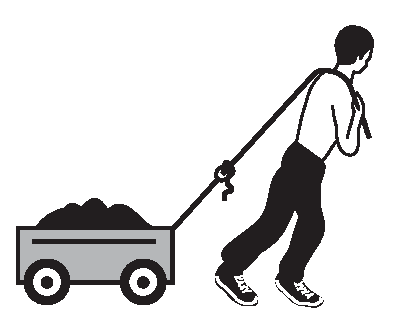
\includegraphics[keepaspectratio,scale=0.75]{Jan2003-Q01}
    \end{center}
    The worker's pull on the handle of the cart can best be described as a force having:
    \begin{choices}
      \correctchoice{both magnitude and direction}
        \wrongchoice{magnitude, only}
        \wrongchoice{direction, only}
        \wrongchoice{neither magnitude nor direction}
    \end{choices}
\end{question}
}

\element{nysed}{
\begin{question}{Jan2003-Q04}
    The sum of all forces acting on a moving object is zero,
        the object will:
    \begin{choices}
      \correctchoice{continue moving with constant velocity}
        \wrongchoice{slow down and stop}
        \wrongchoice{change the direction of its motion}
        \wrongchoice{accelerate uniformly}
    \end{choices}
\end{question}
}

\element{nysed}{
\begin{question}{Jan2003-Q05}
    A net force of \SI{10}{\newton} accelerates an object at \SI{5.0}{\meter\per\second\squared}.
    What net force would be required to accelerate the same object at \SI{1.0}{\meter\per\second\squared}?
    \begin{multicols}{2}
    \begin{choices}
      \correctchoice{\SI{2.0}{\newton}}
        \wrongchoice{\SI{1.0}{\newton}}
        \wrongchoice{\SI{5.0}{\newton}}
        \wrongchoice{\SI{50}{\newton}}
    \end{choices}
    \end{multicols}
\end{question}
}

\element{nysed}{
\begin{question}{Jan2003-Q07}
    A \SI{1200}{\kilo\gram} car traveling at \SI{10}{\meter\per\second} hits a tree and is brought to rest in \SI{0.10}{\second}.
    What is the magnitude of the average force acting on the car to bring it to rest?
    \begin{multicols}{2}
    \begin{choices}
      \correctchoice{\SI{1.2e5}{\newton}}
        \wrongchoice{\SI{1.2e4}{\newton}}
        \wrongchoice{\SI{1.2e3}{\newton}}
        \wrongchoice{\SI{1.2e2}{\newton}}
    \end{choices}
    \end{multicols}
\end{question}
}

\element{nysed}{
\begin{question}{Jan2003-Q08}
    A spring scale reads \SI{20}{\newton} as it pulls a \SI{5.0}{\kilo\gram} mass across a table.
    What is the magnitude of the force exerted by the mass on the spring scale?
    \begin{multicols}{2}
    \begin{choices}
      \correctchoice{\SI{20}{\newton}}
        \wrongchoice{\SI{49}{\newton}}
        \wrongchoice{\SI{3.0}{\newton}}
        \wrongchoice{\SI{4.0}{\newton}}
    \end{choices}
    \end{multicols}
\end{question}
}

\element{nysed}{
\begin{question}{Jan2003-Q37}
    The diagram below shows a force of magnitude $F$ applied to a mass at angle $\theta$ relative to a horizontal frictionless surface.
    \begin{center}
    \begin{tikzpicture}[font=\footnotesize]
        %% Block
        \draw[thick] (-2,0) rectangle (0,1);
        \node[anchor=center] at (-1.0,0.5) {mass};
        %% Force 1
        \draw[dashed,thick] (0,0.5) -- (2.00,0.5)
            node[pos=0.5,anchor=north] {horizontal};
        \draw[thick,->] (0,0.5) -- ++(30:2)
            node[pos=0.5,anchor=south] {$F$};
        \draw[thick,dashed,<->] (1.0,0.5) arc (0:30:1.0)
            node[pos=0.5,anchor=west] {$\theta$};
        %% Floor
        \draw[thick] (-3,0) -- (3,0);
        \foreach \x in {-30,-29,...,30}
            \draw[thin] (\x mm,0cm) -- ++ (220:0.20cm);
        \node[anchor=north] at (0,-0.20) {Frictionless surface};
    \end{tikzpicture}
    \end{center}
    As angle $\theta$ is increased, the horizontal acceleration of the mass:
    \begin{choices}
      \correctchoice{decreases}
        \wrongchoice{increases}
        \wrongchoice{remains the same}
    \end{choices}
\end{question}
}


%% Section Aug2002
%%--------------------
\element{nysed}{
\begin{question}{Aug2002-Q01}
    A net force of \SI{25}{\newton} is applied horizontally to a \SI{10}{\kilo\gram} block resting on a table.
    What is the magnitude of the acceleration of the block?
    \begin{multicols}{2}
    \begin{choices}
        \wrongchoice{\SI{0.0}{\meter\per\second\squared}}
        \wrongchoice{\SI{0.26}{\meter\per\second\squared}}
        \wrongchoice{\SI{0.40}{\meter\per\second\squared}}
      \correctchoice{\SI{2.5}{\meter\per\second\squared}}
    \end{choices}
    \end{multicols}
\end{question}
}

\element{nysed}{
\begin{question}{Aug2002-Q06}
    If the magnitude of the gravitational force of Earth on the Moon is $F$,
        the magnitude of the gravitational force of the Moon on Earth is:
    \begin{choices}
        \wrongchoice{smaller than $F$}
        \wrongchoice{larger than $F$}
      \correctchoice{equal to $F$}
    \end{choices}
\end{question}
}

\element{nysed}{
\begin{question}{Aug2002-Q27}
    During a collision, an \SI{84}{\kilo\gram} driver of a car moving at \SI{24}{\meter\per\second} is brought to rest by an inflating air bag in \SI{1.2}{\second}.
    The magnitude of the force exerted on the driver by the air bag is approximately:
    \begin{multicols}{2}
    \begin{choices}
        \wrongchoice{\SI{7.0e1}{\newton}}
        \wrongchoice{\SI{8.2e2}{\newton}}
      \correctchoice{\SI{1.7e3}{\newton}}
        \wrongchoice{\SI{2.0e3}{\newton}}
    \end{choices}
    \end{multicols}
\end{question}
}

\element{nysed}{
\begin{question}{Aug2002-Q28}
    An apple weighing \SI{1}{\newton} on the surface of Earth has a mass of approximately:
    \begin{multicols}{2}
    \begin{choices}
      \correctchoice{\SI{e-1}{\kilo\gram}}
        \wrongchoice{\SI{e0}{\kilo\gram}}
        \wrongchoice{\SI{e1}{\kilo\gram}}
        \wrongchoice{\SI{e2}{\kilo\gram}}
    \end{choices}
    \end{multicols}
\end{question}
}

\element{nysed}{
\begin{question}{Aug2002-Q31}
    In which situation is the net force on the object equal to zero?
    \begin{choices}
        \wrongchoice{a satellite moving at constant speed around Earth in a circular orbit}
        \wrongchoice{an automobile braking to a stop}
      \correctchoice{a bicycle moving at constant speed on a straight, level road}
        \wrongchoice{a pitched baseball being hit by a bat}
    \end{choices}
\end{question}
}


%% Section June2002
%%--------------------
\element{nysed}{
\begin{question}{June2002-Q07}
    A \SI{70}{\kilo\gram} astronaut has a weight of \SI{560}{\newton} on the surface of planet Alpha.
    What is the acceleration due to gravity on planet Alpha?
    \begin{multicols}{2}
    \begin{choices}
        \wrongchoice{\SI{0.0}{\meter\per\second\squared}}
        \wrongchoice{\SI{8.0}{\meter\per\second\squared}}
        \wrongchoice{\SI{9.8}{\meter\per\second\squared}}
      \correctchoice{\SI{80}{\meter\per\second\squared}}
    \end{choices}
    \end{multicols}
\end{question}
}

\element{nysed}{
\begin{question}{June2002-Q10}
    The diagram below shows a horizontal \SI{8.0}{\newton} force applied to a \SI{4.0}{\kilo\gram} block on a frictionless table.
    \begin{center}
    \begin{tikzpicture}
        %% Block
        \draw[thick] (-2,0) rectangle (0,1);
        \node[anchor=center] at (-1.0,0.5) {\SI{4.0}{\kilo\gram}};
        %% Force 1
        \draw[thick,->] (0,0.5) -- (2.00,0.5)
            node[pos=1.0,anchor=south east] {$F=\SI{8.0}{\newton}$};
        %% Floor
        \draw[thick] (-3,0) -- (3,0);
        \foreach \x in {-30,-29,...,30}
            \draw[thin] (\x mm,0cm) -- ++ (220:0.20cm);
        \node[anchor=north] at (0,-0.20) {Frictionless surface};
    \end{tikzpicture}
    \end{center}
    What is the magnitude of the block's acceleration?
    \begin{multicols}{2}
    \begin{choices}
        \wrongchoice{\SI{0.50}{\meter\per\second\squared}}
      \correctchoice{\SI{2.0}{\meter\per\second\squared}}
        \wrongchoice{\SI{9.8}{\meter\per\second\squared}}
        \wrongchoice{\SI{32}{\meter\per\second\squared}}
    \end{choices}
    \end{multicols}
\end{question}
}

\newcommand{\nysedJuneTwentyZeroTwoQTwelve}{
\begin{tikzpicture}
    %% Ground
    \node[anchor=north,fill,pattern=north east lines,minimum width=8cm, minimum height=0.05cm] at (0,0) {};
    \draw (-4,0) -- (4,0);
    %% carts
    \node[draw,minimum width=2cm,minimum height=2em,anchor=south] (A) at (-2,0.3) {\SI{2}{\kilo\gram}};
    \node[draw,minimum width=1cm,minimum height=2em,anchor=south] (B) at (2,0.3) {\SI{1}{\kilo\gram}};
    \node[anchor=south] at (A.north) {$A$};
    \node[anchor=south] at (B.north) {$B$};
    %% wheels
    \draw[fill=white!90!black] (A.south west) ++(0:0.2cm) arc(90:-270:0.15);
    \draw[fill=white!90!black] (A.south east) ++(180:0.2cm) arc(90:-270:0.15);
    \draw[fill=white!90!black] (B.south west) ++(0:0.2cm) arc(90:-270:0.15);
    \draw[fill=white!90!black] (B.south east) ++(180:0.2cm) arc(90:-270:0.15);
    %% Spring
    \draw[decoration={aspect=0.2,segment length=1.5mm,amplitude=2mm,coil},decorate] (A.east) -- (B.west);
    \draw[thick] (A.north east) -- (B.north west);
\end{tikzpicture}
}

\element{nysed}{
\begin{question}{June2002-Q12}
    The diagram shows a compressed spring between two carts initially at rest on a horizontal frictionless surface.
    Cart $A$ has a mass of 2 kilograms and cart $B$ has a mass of \SI{1}{\kilo\gram}.
    A string holds the carts together.
    \begin{center}
        \nysedJuneTwentyZeroTwoQTwelve
    \end{center}
    What occurs when the string is cut and the carts move apart?
    \begin{choices}
      \correctchoice{The magnitude of the acceleration of cart $A$ is one-half the magnitude of the acceleration of cart $B$.}
        \wrongchoice{The length of time that the force acts on cart $A$ is twice the length of time the force acts on cart $B$.}
        \wrongchoice{The magnitude of the force exerted on cart $A$ is one-half the magnitude of the force exerted on cart $B$.}
        \wrongchoice{The magnitude of the impulse applied to cart $A$ is twice the magnitude of the impulse applied to cart $B$.}
    \end{choices}
\end{question}
}

\element{nysed}{
\begin{question}{June2002-Q13}
    The diagram shows a compressed spring between two carts initially at rest on a horizontal frictionless surface.
    Cart $A$ has a mass of 2 kilograms and cart $B$ has a mass of \SI{1}{\kilo\gram}.
    A string holds the carts together.
    \begin{center}
        \nysedJuneTwentyZeroTwoQTwelve
    \end{center}
    After the string is cut and the two carts move apart,
        the magnitude of which quantity is the same for both carts?
    \begin{multicols}{2}
    \begin{choices}
      \correctchoice{momentum}
        \wrongchoice{inertia}
        \wrongchoice{velocity}
        \wrongchoice{kinetic energy}
    \end{choices}
    \end{multicols}
\end{question}
}


%% Section Jan2002
%%--------------------
\element{nysed}{
\begin{question}{Jan2002-Q07}
    A \SI{4.0}{\kilo\gram} rock and a \SI{1.0}{\kilo\gram} stone fall freely from rest from a height of \SI{100}{\meter}.
    After they fall for \SI{2.0}{\second},
        the ratio of the rock's speed to the stone's speed is:
    \begin{multicols}{2}
    \begin{choices}
      \correctchoice{$1:1$}
        \wrongchoice{$1:2$}
        \wrongchoice{$2:1$}
        \wrongchoice{$4:1$}
    \end{choices}
    \end{multicols}
\end{question}
}

\element{nysed}{
\begin{question}{Jan2002-Q09}
    In the diagram below,
        a box is on a frictionless horizontal surface with forces $F_1$ and $F_2$ acting as shown.
    \begin{center}
    \begin{tikzpicture}
        %% Block
        \draw[thick] (-1,0) rectangle (1,1);
        \node[anchor=center] at (0,0.5) {Box};
        %% Force 1
        \draw[thick,->] (1,0.5) -- (3.00,0.5)
            node[pos=1.0,anchor=south east] {$F_1$};
        %% Force 2
        \draw[thick,->] (-1,0.5) -- (-3.00,0.5)
            node[pos=1.0,anchor=south west] {$F_2$};
        %% Floor
        \draw[thick] (-3,0) -- (3,0);
        \foreach \x in {-30,-28,...,30}
            \draw[thin] (\x mm,0cm) -- ++ (220:0.20cm);
        \node[anchor=north] at (0,-0.20) {Frictionless surface};
    \end{tikzpicture}
    \end{center}
    If the magnitude of $F_1$ is greater than the magnitude of $F_2$,
        then the box is:
    \begin{choices}
        \wrongchoice{moving at constant speed in the direction of $F_1$}
        \wrongchoice{moving at constant speed in the direction of $F_2$}
      \correctchoice{accelerating in the direction of $F_1$}
        \wrongchoice{accelerating in the direction of $F_2$}
    \end{choices}
\end{question}
}

\element{nysed}{
\begin{question}{Jan2002-Q11}
    Which pair of displacement ($d$) and velocity ($v$) graphs best represent the motion of an object on which the net force is zero?
    \begin{choices}
        \AMCboxDimensions{down=-2.5em}
        \correctchoice{
            \begin{tikzpicture}
                \begin{groupplot}[
                    axis lines=middle,
                    axis line style={->},
                    group style={group size=2 by 1},
                    xtick=\empty,
                    x label style={
                        at={(current axis.right of origin)},
                        anchor=west,
                        font=\normalsize,
                    },
                    xmin=0,xmax=10,
                    ytick=\empty,
                    y label style={
                        at={(current axis.above origin)},
                        anchor=south,
                        font=\normalsize,
                    },
                    ymin=0,ymax=10,
                    width=0.5\columnwidth,
                    ]
                    \nextgroupplot[
                        xlabel={$t$},
                        ylabel={$d$},
                    ] \addplot[line width=1pt,domain=0:10] {x};
                    \nextgroupplot[
                        xlabel={$t$},
                        ylabel={$v$},
                    ] \addplot[line width=1pt,domain=0:10] {8};
                \end{groupplot}
            \end{tikzpicture}
        }
        \wrongchoice{
            \begin{tikzpicture}
                \begin{groupplot}[
                    axis lines=middle,
                    axis line style={->},
                    group style={group size=2 by 1},
                    xtick=\empty,
                    x label style={
                        at={(current axis.right of origin)},
                        anchor=west,
                        font=\normalsize,
                    },
                    xmin=0,xmax=10,
                    ytick=\empty,
                    y label style={
                        at={(current axis.above origin)},
                        anchor=south,
                        font=\normalsize,
                    },
                    ymin=0,ymax=10,
                    width=0.5\columnwidth,
                    ]
                    \nextgroupplot[
                        xlabel={$t$},
                        ylabel={$d$},
                    ] \addplot[line width=1pt,domain=0:10] {0.1 * x * x};
                    \nextgroupplot[
                        xlabel={$t$},
                        ylabel={$v$},
                    ] \addplot[line width=1pt,domain=0:10] {x};
                \end{groupplot}
            \end{tikzpicture}
        }
        \wrongchoice{
            \begin{tikzpicture}
                \begin{groupplot}[
                    axis lines=middle,
                    axis line style={->},
                    group style={group size=2 by 1},
                    xtick=\empty,
                    x label style={
                        at={(current axis.right of origin)},
                        anchor=west,
                        font=\normalsize,
                    },
                    xmin=0,xmax=10,
                    ytick=\empty,
                    y label style={
                        at={(current axis.above origin)},
                        anchor=south,
                        font=\normalsize,
                    },
                    ymin=0,ymax=10,
                    width=0.5\columnwidth,
                    ]
                    \nextgroupplot[
                        xlabel={$t$},
                        ylabel={$d$},
                    ] \addplot[line width=1pt,domain=0:10] {x};
                    \nextgroupplot[
                        xlabel={$t$},
                        ylabel={$v$},
                    ] \addplot[line width=1pt,domain=0:10] {0.5*x};
                \end{groupplot}
            \end{tikzpicture}
        }
        \wrongchoice{
            \begin{tikzpicture}
                \begin{groupplot}[
                    axis lines=middle,
                    axis line style={->},
                    group style={group size=2 by 1},
                    xtick=\empty,
                    x label style={
                        at={(current axis.right of origin)},
                        anchor=west,
                        font=\normalsize,
                    },
                    xmin=0,xmax=10,
                    ytick=\empty,
                    y label style={
                        at={(current axis.above origin)},
                        anchor=south,
                        font=\normalsize,
                    },
                    ymin=0,ymax=10,
                    width=0.5\columnwidth,
                    ]
                    \nextgroupplot[
                        xlabel={$t$},
                        ylabel={$d$},
                    ] \addplot[line width=1pt,domain=0:10] {0.1 * x * x};
                    \nextgroupplot[
                        xlabel={$t$},
                        ylabel={$v$},
                    ] \addplot[line width=1pt,domain=0:10] {8};
                \end{groupplot}
            \end{tikzpicture}
        }
    \end{choices}
\end{question}
}

\element{nysed}{
\begin{question}{Jan2002-Q13}
    The magnitude of the force that a baseball bat exerts on a ball is \SI{50}{\newton}.
    The magnitude of the force that the ball exerts on the bat is:
    \begin{multicols}{2}
    \begin{choices}
        \wrongchoice{\SI{5.0}{\newton}}
        \wrongchoice{\SI{10}{\newton}}
      \correctchoice{\SI{50}{\newton}}
        \wrongchoice{\SI{250}{\newton}}
    \end{choices}
    \end{multicols}
\end{question}
}

\element{nysed}{
\begin{question}{Jan2002-Q16}
    What is an essential characteristic of an object in equilibrium?
    \begin{choices}
        \wrongchoice{zero velocity}
      \correctchoice{zero acceleration}
        \wrongchoice{zero potential energy}
        \wrongchoice{zero kinetic energy}
    \end{choices}
\end{question}
}


%% Section June2001
%%--------------------
\element{nysed}{
\begin{question}{June2001-Q07}
    In an automobile collision, a \SI{44}{\kilo\gram} passenger moving at \SI{15}{\meter\per\second} is brought to rest by an air bag during a \SI{0.10}{\second} time interval.
    What is the magnitude of the average force exerted on the passenger during this time?
    \begin{multicols}{2}
    \begin{choices}
        \wrongchoice{\SI{440}{\newton}}
        \wrongchoice{\SI{660}{\newton}}
        \wrongchoice{\SI{4400}{\newton}}
      \correctchoice{\SI{6600}{\newton}}
    \end{choices}
    \end{multicols}
\end{question}
}

\element{nysed}{
\begin{question}{June2001-Q08}
    A series of unbalanced forces was applied to each of two blocks, $A$ and $B$.
    The graphs below show the relationship between unbalanced force and acceleration for each block.
    \begin{center}
    \begin{tikzpicture}
        \begin{groupplot}[
            axis y line=left,
            axis x line=bottom,
            axis line style={->},
            group style={group size=2 by 1},
            xtick={0,1,2,3,4},
            xlabel={acceleration},
            x unit=\si{\meter\per\second\squared},
            xmin=0,xmax=4.5,
            ytick={0,1,2,3},
            ylabel={force},
            y unit=\si{\newton},
            ymin=0,ymax=3.5,
            width=0.5\columnwidth,
            ]
            \nextgroupplot[title={Block $A$}]
            \addplot[line width=1pt,domain=0:3.5] {x};
            \addplot[mark=*] coordinates {(1,1) (2,2) (3,3)};
            \nextgroupplot[title={Block $B$}]
            \addplot[line width=1pt,domain=0:2] {2*x};
            \addplot[mark=*] coordinates {(0.5,1) (1,2) (1.5,3)};
        \end{groupplot}
    \end{tikzpicture}
    \end{center}
    Compared to the mass of block $A$,
        the mass of block $B$ is:
    \begin{multicols}{2}
    \begin{choices}
        \wrongchoice{the same}
      \correctchoice{twice as great}
        \wrongchoice{half as great}
        \wrongchoice{four times as great}
    \end{choices}
    \end{multicols}
\end{question}
}

\element{nysed}{
\begin{question}{June2001-Q55}
    A mosquito flying over a highway strikes the windshield of a moving truck.
    Compared to the magnitude of the force of the truck on the mosquito during the collision,
        the magnitude of the force of the mosquito on the truck is:
    \begin{multicols}{3}
    \begin{choices}
        \wrongchoice{smaller}
        \wrongchoice{larger}
      \correctchoice{the same}
    \end{choices}
    \end{multicols}
\end{question}
}


%% Section Jan2001
%%--------------------
\element{nysed}{
\begin{question}{Jan2001-Q08}
    Which is a derived unit?
    \begin{multicols}{2}
    \begin{choices}
        \wrongchoice{meter (\si{\meter})}
        \wrongchoice{kilogram (\si{\kilo\gram})}
        \wrongchoice{second (\si{\kilo\gram})}
      \correctchoice{newton (\si{\newton})}
    \end{choices}
    \end{multicols}
\end{question}
}

\element{nysed}{
\begin{question}{Jan2001-Q13}
    A \SI{2.0}{\kilo\gram} mass weights \SI{10}{\newton} on planet $X$.
    The acceleration due to gravity on planet $X$ is approximately:
    \begin{multicols}{2}
    \begin{choices}
        \wrongchoice{\SI{0.20}{\meter\per\second\squared}}
      \correctchoice{\SI{5.0}{\meter\per\second\squared}}
        \wrongchoice{\SI{9.8}{\meter\per\second\squared}}
        \wrongchoice{\SI{20}{\meter\per\second\squared}}
    \end{choices}
    \end{multicols}
\end{question}
}


%% Section June2000
%%--------------------
\element{nysed}{
\begin{question}{June2000-Q12}
    Two forces are applied to a \SI{2.0}{\kilo\gram} block on a frictionless horizontal surface,
        as shown in the diagram below.
    [Vectors are drawn to scale]
    \begin{center}
    \begin{tikzpicture}
        %% Force 1
        \draw[thick,->] (-0,0.5) -- (-2.66,0.5)
            node[pos=1.0,anchor=south west] {$F_1=\SI{8}{\newton}$};
        %% Force 2
        \draw[thick,->] (2,0.5) -- (3.00,0.5)
            node[pos=0.0,anchor=south west] {$F_2=\SI{3}{\newton}$};
        %% Block
        \draw[thick] (0,0) rectangle (2,1);
        \node[anchor=center] at (1,0.5) {\SI{2.0}{\kilo\gram}};
        %% Floor
        \draw[thick] (-3,0) -- (3,0);
        \foreach \x in {-30,-29,...,30}
            \draw[thin] (\x mm,0cm) -- ++ (220:0.15cm);
        \node[anchor=north] at (0,-0.15) {Frictionless surface};
    \end{tikzpicture}
    \end{center}
    The acceleration of the block is:
    \begin{choices}
        \wrongchoice{\SI{1.5}{\meter\per\second\squared} to the right}
      \correctchoice{\SI{2.5}{\meter\per\second\squared} to the left}
        \wrongchoice{\SI{2.5}{\meter\per\second\squared} to the right}
        \wrongchoice{\SI{4.0}{\meter\per\second\squared} to the left}
    \end{choices}
\end{question}
}

\element{nysed}{
\begin{question}{June2000-Q13}
    A \SI{15}{\kilo\gram} mass weighs \SI{60}{\newton} on planet $X$.
    The mass is allowed to fall freely from rest near the surface of the planet.
    After falling for \SI{6.0}{\second},
        the acceleration of the mass is:
    \begin{multicols}{2}
    \begin{choices}
        \wrongchoice{\SI{0.25}{\meter\per\second\squared}}
        \wrongchoice{\SI{10}{\meter\per\second\squared}}
        \wrongchoice{\SI{24}{\meter\per\second\squared}}
      \correctchoice{\SI{4.0}{\meter\per\second\squared}}
    \end{choices}
    \end{multicols}
\end{question}
}

\element{nysed}{
\begin{question}{June2000-Q17}
    A \SI{2 400}{\kilo\gram} car is traveling at a speed of \SI{20}{\meter\per\second}.
    Compared to the magnitude of the force required to stop the car in \SI{12}{\second},
        the magnitude of the force required to stop the car in \SI{6}{\second} is:
    \begin{choices}
        \wrongchoice{half as great}
      \correctchoice{twice as great}
        \wrongchoice{the same}
        \wrongchoice{four times as great}
    \end{choices}
\end{question}
}


%% Section June1999
%%--------------------
\element{nysed}{
\begin{question}{June1999-Q04}
    A \SI{1.2e3}{\kilo\gram} car is accelerated uniformly from \SI{10}{\meter\per\second} to \SI{20}{\meter\per\second} in \SI{5.0}{\second}.
    What is the magnitude of the net force acting on the car during this \SI{5.0}{\second} interval?
    \begin{multicols}{2}
    \begin{choices}
      \correctchoice{\SI{2.4e3}{\newton}}
        \wrongchoice{\SI{4.8e3}{\newton}}
        \wrongchoice{\SI{7.2e3}{\newton}}
        \wrongchoice{\SI{1.2e4}{\newton}}
    \end{choices}
    \end{multicols}
\end{question}
}

\element{nysed}{
\begin{question}{June1999-Q09}
    The diagram below shows a student applying a \SI{10}{\newton} force to slide a piece of wood at constant speed across a horizontal surface.
    After the wood is cut in half,
        one piece is placed on top of the other, as shown.
    \begin{center}
    \begin{tikzpicture}
        %% NOTE: add picture
    \end{tikzpicture}
    \end{center}
    What is the magnitude of the force, $F$,
        required to slide the stacked wood at constant speed across the surface?
    \begin{multicols}{2}
    \begin{choices}
        \wrongchoice{\SI{40}{\newton}}
        \wrongchoice{\SI{20}{\newton}}
      \correctchoice{\SI{10}{\newton}}
        \wrongchoice{\SI{5.0}{\newton}}
    \end{choices}
    \end{multicols}
\end{question}
}

\element{nysed}{
\begin{question}{June1999-Q11}
    Which combination of fundamental units can be used to express the weight of an object?
    \begin{choices}
        \wrongchoice{kilogram per second (\si{\kilo\gram\per\second})}
        \wrongchoice{kilogram meter (\si{\kilo\gram\meter})}
        \wrongchoice{kilogram meter per second (\si{\kilo\gram\meter\per\second})}
      \correctchoice{kilogram meter per second squared (\si{\kilo\gram\meter\per\second\squared})}
    \end{choices}
\end{question}
}

\element{nysed}{
\begin{question}{June1999-Q15}
    The diagram below shows a child pulling a \SI{50}{\kilo\gram} friend on a sled by applying a \SI{300}{\newton} force on the sled rope at an angle of \ang{40} with the horizontal.
    \begin{center}
        %% NOTE: too complex for tikz
        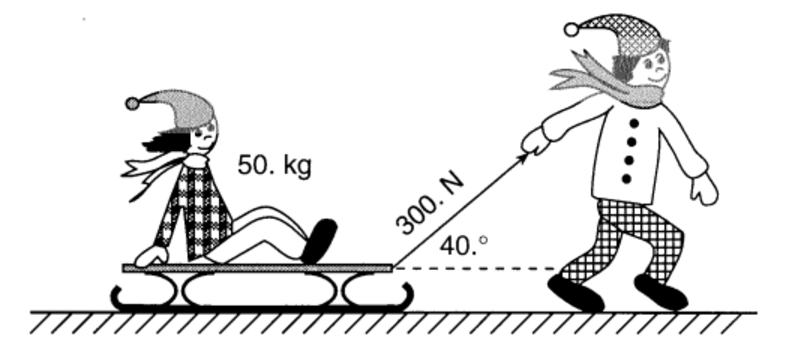
\includegraphics[keepaspectratio,scale=0.5]{June1999-Q15}
    \end{center}
    The vertical component of the \SI{300}{\newton} force is approximately:
    \begin{multicols}{2}
    \begin{choices}
        \wrongchoice{\SI{510}{\newton}}
        \wrongchoice{\SI{230}{\newton}}
      \correctchoice{\SI{190}{\newton}}
        \wrongchoice{\SI{32}{\newton}}
    \end{choices}
    \end{multicols}
\end{question}
}

\element{nysed}{
\begin{question}{June1999-Q17}
    A \SI{6.0}{\newton} force and a \SI{8}{\newton} force act concurrently on a box located on a frictionless horizontal surface.
    Which top-view diagram shows the forces producing the \emph{smallest} magnitude of acceleration of the box?
    \begin{multicols}{2}
    \begin{choices}[o]
        \footnotesize
        \AMCboxDimensions{down=-1.1cm}
        \correctchoice{
            \begin{tikzpicture}[scale=0.8]
                \draw[white!60!black,dashed] (-1.8,-2.0) rectangle (2.10,1.5);
                %% Block
                \node[draw,rectangle,minimum size=1cm,text centered,text width=1cm]
                    (B) at (0,0) {Top of Block};
                %% 8 Newton
                \draw[thick,->] (B.east) -- ++(0:1.33cm)
                    node[pos=1.0,anchor=south east] {\SI{8.0}{\newton}};
                %% 6 Newton
                \draw[thick,->] (B.west) -- ++(180:1.00cm)
                    node[pos=1.0,anchor=south west] {\SI{6.0}{\newton}};
            \end{tikzpicture}
        }
        \wrongchoice{
            \begin{tikzpicture}[scale=0.8]
                \draw[white!60!black,dashed] (-1.8,-2.0) rectangle (2.10,1.5);
                %% Block
                \node[draw,rectangle,minimum size=1cm,text centered,text width=1cm]
                    (B) at (0,0) {Top of Block};
                %% 8 Newton
                \draw[thick,->] (B.east) -- ++(0:1.33cm)
                    node[pos=1.0,anchor=south east] {\SI{8.0}{\newton}};
                %% 6 Newton
                \draw[thick,->] (B.south) -- ++(270:1.00cm)
                    node[pos=1.0,anchor=south west] {\SI{6.0}{\newton}};
            \end{tikzpicture}
        }
        \wrongchoice{
            \begin{tikzpicture}[scale=0.8]
                \draw[white!60!black,dashed] (-1.8,-2.0) rectangle (2.10,1.5);
                %% Block
                \node[draw,rectangle,minimum size=1cm,text centered,text width=1cm]
                    (B) at (0,0) {Top of Block};
                %% 8 Newton
                \draw[thick,->] (B.south) -- ++(270:1.33cm)
                    node[pos=1.0,anchor=south west] {\SI{8.0}{\newton}};
                %% 6 Newton
                \draw[thick,->] (B.west) -- ++(200:1.00cm)
                    node[pos=1.0,anchor=south west,rotate=20] {\SI{6.0}{\newton}};
            \end{tikzpicture}
        }
        \wrongchoice{
            \begin{tikzpicture}[scale=0.8]
                \draw[white!60!black,dashed] (-1.8,-2.0) rectangle (2.10,1.5);
                %% Block
                \node[draw,rectangle,minimum size=1cm,text centered,text width=1cm]
                    (B) at (0,0) {Top of Block};
                %% 8 Newton
                \draw[thick,->] (B.south)++(10pt,0) -- ++(270:1.33cm)
                    node[pos=0.5,anchor=west] {\SI{8.0}{\newton}};
                %% 6 Newton
                \draw[thick,->] (B.south)++(-10pt,0) -- ++(270:1.00cm)
                    node[pos=0.5,anchor=east] {\SI{6.0}{\newton}};
            \end{tikzpicture}
        }
    \end{choices}
    \end{multicols}
\end{question}
}


%% Section June1998
%%--------------------
\element{nysed}{
\begin{question}{June1998-Q08}
    A man weighs \SI{900}{\newton} standing on a scale in a stationary elevator.
    If some time later the reading on the scale is \SI{1200}{\newton},
        the elevator must be moving with:
    \begin{choices}
        \wrongchoice{constant acceleration downward}
        \wrongchoice{constant speed downward}
      \correctchoice{constant acceleration upward}
        \wrongchoice{constant speed upward}
    \end{choices}
\end{question}
}

\element{nysed}{
\begin{question}{June1998-Q09}
    Net force $F$ causes $m_1$ to accelerate at rate $a$.
    A net force of $3F$ causes mass $m_2$ to accelerate at rate $2a$.
    What is the ratio of mass $m_1$ to mass $m_2$?
    \begin{multicols}{2}
    \begin{choices}
        \wrongchoice{$1:3$}
      \correctchoice{$2:3$}
        \wrongchoice{$1:2$}
        \wrongchoice{$1:6$}
    \end{choices}
    \end{multicols}
\end{question}
}

\element{nysed}{
\begin{question}{June1998-Q13}
    A \SI{0.60}{\kilo\gram} softball initially at rest is hit with a bat.
    The ball is in contact with the bat for \SI{0.20}{\second} and leaves the bat with a speed of \SI{25}{\meter\per\second}.
    What is the magnitude of the average force exerted by the ball on the bat?
    \begin{multicols}{2}
    \begin{choices}
        \wrongchoice{\SI{8.3}{\newton}}
        \wrongchoice{\SI{15}{\newton}}
        \wrongchoice{\SI{3.0}{\newton}}
      \correctchoice{\SI{75}{\newton}}
    \end{choices}
    \end{multicols}
\end{question}
}

\element{nysed}{
\begin{question}{June1998-Q16}
    A person kicks a \SI{4.0}{\kilo\gram} door with a \SI{48}{\newton} force causing the door to accelerate at \SI{12}{\meter\per\second\squared}.
    What is the magnitude of the force exerted by the door on the person?
    \begin{multicols}{2}
    \begin{choices}
      \correctchoice{\SI{48}{\newton}}
        \wrongchoice{\SI{24}{\newton}}
        \wrongchoice{\SI{12}{\newton}}
        \wrongchoice{\SI{4.0}{\newton}}
    \end{choices}
    \end{multicols}
\end{question}
}


%% Section June1997
%%--------------------
\element{nysed}{
\begin{question}{June1997-Q05}
    A \SI{150}{\newton} force, $F_1$, and a \SI{200}{\newton} force,
        $F_2$, are applied simultaneously to the same point on a large crate resting on a frictionless, horizontal surface.
    Which diagram shows the forces positioned to give the crate the greatest acceleration?
    [Vectors are drawn to scale]
    \begin{multicols}{2}
    \begin{choices}
        \AMCboxDimensions{down=-0.25cm}
        \correctchoice{
            \begin{tikzpicture}[scale=0.75]
                \draw[white] (-2,-0.5) rectangle (2,2.33);
                %% Block
                \node[draw,rectangle,minimum size=0.8cm,anchor=south] (B) at (-0.5,0) {};
                %% F_1
                \draw[thick,->] (B.north east) -- ++(0:1.25)
                    node[pos=1.0,anchor=south east] {$F_1$};
                %% F_2
                \draw[thick,->] (B.east) -- ++(0:1.66)
                    node[pos=1.0,anchor=south] {$F_2$};
                %% Floor
                \draw[thick] (-2,0) -- (2,0);
                \node[anchor=north,pattern=north east lines,minimum width=3cm] at (0,0) {};
            \end{tikzpicture}
        }
        \wrongchoice{
            \begin{tikzpicture}[scale=0.75]
                \draw[white] (-2,-0.5) rectangle (2,2.33);
                %% Block
                \node[draw,rectangle,minimum size=0.8cm,anchor=south] (B) at (-0.5,0) {};
                %% F_1
                \draw[thick,<-] (B.north) -- ++(90:1.25)
                    node[pos=0.0,anchor=south east] {$F_1$};
                %% F_2
                \draw[thick,->] (B.east) -- ++(0:1.66)
                    node[pos=1.0,anchor=south east] {$F_2$};
                %% Floor
                \draw[thick] (-2,0) -- (2,0);
                \node[anchor=north,pattern=north east lines,minimum width=3cm] at (0,0) {};
            \end{tikzpicture}
        }
        \wrongchoice{
            \begin{tikzpicture}[scale=0.75]
                \draw[white] (-2,-0.5) rectangle (2,2.33);
                %% Block
                \node[draw,rectangle,minimum size=0.8cm,anchor=south] (B) at (-0.5,0) {};
                %% F_1
                \draw[thick,->] (B.north) -- ++(90:1.25)
                    node[pos=1.0,anchor=north east] {$F_1$};
                %% F_2
                \draw[thick,->] (B.east) -- ++(0:1.66)
                    node[pos=1.0,anchor=south east] {$F_2$};
                %% Floor
                \draw[thick] (-2,0) -- (2,0);
                \node[anchor=north,pattern=north east lines,minimum width=3cm] at (0,0) {};
            \end{tikzpicture}
        }
        \wrongchoice{
            \begin{tikzpicture}[scale=0.75]
                \draw[white] (-2,-0.5) rectangle (2,2.33);
                %% Block
                \node[draw,rectangle,minimum size=0.8cm,anchor=south] (B) at (-0.5,0) {};
                %% F_1
                \draw[thick,->] (B.west) -- ++(180:1.25)
                    node[pos=1.0,anchor=south west] {$F_1$};
                %% F_2
                \draw[thick,->] (B.east) -- ++(0:1.66)
                    node[pos=1.0,anchor=south east] {$F_2$};
                %% Floor
                \draw[thick] (-2,0) -- (2,0);
                \node[anchor=north,pattern=north east lines,minimum width=3cm] at (0,0) {};
            \end{tikzpicture}
        }
    \end{choices}
    \end{multicols}
\end{question}
}

\element{nysed}{
\begin{question}{June1997-Q11}
    The graph below shows the weight of three objects on planet $X$ as a function of their mass.
    \begin{center}
    \begin{tikzpicture}
        \begin{axis}[
            axis y line=left,
            axis x line=bottom,
            axis line style={->},
            ylabel={Weight},
            y unit=\si{\newton},
            ytick={0,100,200,300,400,500},
            xlabel={Mass},
            x unit=\si{\kilo\gram},
            xtick={0,25,50,75},
            xmin=0,xmax=77,
            ymin=0,ymax=510,
            grid=major,
            width=0.8\columnwidth,
            height=0.5\columnwidth,
            very thin,
        ]
        \addplot[line width=1pt,domain=0:75]{6.0* x};
        \addplot[mark=*] coordinates {(25,150) (50,300) (75,450)};
        \end{axis}
    \end{tikzpicture}
    \end{center}
    The acceleration due to gravity on planet $X$ is approximately:
    \begin{multicols}{2}
    \begin{choices}
        \wrongchoice{\SI{0.17}{\meter\per\second\squared}}
      \correctchoice{\SI{6.0}{\meter\per\second\squared}}
        \wrongchoice{\SI{9.8}{\meter\per\second\squared}}
        \wrongchoice{\SI{50}{\meter\per\second\squared}}
    \end{choices}
    \end{multicols}
\end{question}
}

\element{nysed}{
\begin{question}{June1997-Q12}
    What is the magnitude of the net force acting on a \SI{2.0e3}{\kilo\gram} car as it accelerates from rest to a speed of \SI{15}{\meter\per\second} in \SI{5.0}{\second}?
    \begin{multicols}{2}
    \begin{choices}
      \correctchoice{\SI{6.0e3}{\newton}}
        \wrongchoice{\SI{2.0e4}{\newton}}
        \wrongchoice{\SI{3.0e4}{\newton}}
        \wrongchoice{\SI{6.0e4}{\newton}}
    \end{choices}
    \end{multicols}
\end{question}
}


%% Section June1996
%%--------------------
\element{nysed}{
\begin{question}{June1996-Q07}
    A \SI{0.4}{\kilo\gram} rock and a \SI{1.0}{\kilo\gram} stone fall freely from rest from a height of \SI{100}{\meter}.
    After they fall for \SI{2.0}{\second},
        the ratio of the rock's speed to the stone's speed is:
    \begin{multicols}{2}
    \begin{choices}
      \correctchoice{$1:1$}
        \wrongchoice{$2:1$}
        \wrongchoice{$1:2$}
        \wrongchoice{$4:1$}
    \end{choices}
    \end{multicols}
\end{question}
}

%\element{nysed}{
%\begin{question}{June1996-Q09}
%    The diagram below shows a person exerting a \SI{300}{\newton} force on the handle of a shovel that makes an angle of \ang{60} with the horizontal ground.
%    \begin{center}
%        %% NOTE: picture of a person holding a shovel
%    \end{center}
%    The component of the \SI{300}{\newton} force that acts perpendicular to the ground is approximately:
%    \begin{multicols}{2}
%    \begin{choices}
%        \wrongchoice{\SI{150}{\newton}}
%      \correctchoice{\SI{260}{\newton}}
%        \wrongchoice{\SI{300}{\newton}}
%        \wrongchoice{\SI{350}{\newton}}
%    \end{choices}
%    \end{multicols}
%\end{question}
%}

\element{nysed}{
\begin{question}{June1996-Q10}
    Which graph best represents the motion of an object that has \emph{no} unbalanced force acting on it?
    \begin{multicols}{2}
    \begin{choices}
        \AMCboxDimensions{down=-2.5em}
        \correctchoice{
            \begin{tikzpicture}
                \begin{axis}[
                    axis y line=left,
                    axis x line=bottom,
                    axis line style={->},
                    xlabel={time},
                    xtick=\empty,
                    ylabel={displacement},
                    ytick=\empty,
                    xmin=0,xmax=11,
                    ymin=0,ymax=11,
                    width=1.0\columnwidth,
                ]
                \addplot[line width=1pt,domain=0:10]{0.1*x*x};
                \end{axis}
            \end{tikzpicture}
        }
        \wrongchoice{
            \begin{tikzpicture}
                \begin{axis}[
                    axis y line=left,
                    axis x line=bottom,
                    axis line style={->},
                    xlabel={time},
                    xtick=\empty,
                    ylabel={acceleration},
                    ytick=\empty,
                    xmin=0,xmax=11,
                    ymin=0,ymax=11,
                    width=1.0\columnwidth,
                ]
                \addplot[line width=1pt,domain=0:10]{x};
                \end{axis}
            \end{tikzpicture}
        }
        \wrongchoice{
            \begin{tikzpicture}
                \begin{axis}[
                    axis y line=left,
                    axis x line=bottom,
                    axis line style={->},
                    xlabel={time},
                    xtick=\empty,
                    ylabel={momentum},
                    ytick=\empty,
                    xmin=0,xmax=11,
                    ymin=0,ymax=11,
                    width=1.0\columnwidth,
                ]
                \addplot[line width=1pt,domain=0:10]{x};
                \end{axis}
            \end{tikzpicture}
        }
        \wrongchoice{
            \begin{tikzpicture}
                \begin{axis}[
                    axis y line=left,
                    axis x line=bottom,
                    axis line style={->},
                    xlabel={time},
                    xtick=\empty,
                    ylabel={velocity},
                    ytick=\empty,
                    xmin=0,xmax=11,
                    ymin=0,ymax=11,
                    width=1.0\columnwidth,
                ]
                \addplot[line width=1pt,domain=0:10]{0.1*x*x};
                \end{axis}
            \end{tikzpicture}
        }
    \end{choices}
    \end{multicols}
\end{question}
}

\element{nysed}{
\begin{question}{June1996-Q12}
    Two forces are applied to a \SI{2.0}{\kilo\gram} block on a frictionless,
        horizontal surface, as shown in the diagram below.
    \begin{center}
    \begin{tikzpicture}
        %% Force 1
        \draw[thick,->] (-2.0,0.5) -- (-2.75,0.5)
            node[pos=0.0,anchor=south east] {$F_1=\SI{2}{\newton}$};
        %% Force 2
        \draw[thick,->] (0,0.5) -- (3.0,0.5)
            node[pos=1.0,anchor=south east] at (2,0.5) {$F_2=\SI{8}{\newton}$};
        %% Block
        \draw[thick] (0,0) rectangle (-2,1);
        \node[anchor=center] at (-1,0.5) {\SI{2.0}{\kilo\gram}};
        %% Floor
        \draw[thick] (-3,0) -- (3,0);
        \node[anchor=north,minimum width=6cm,pattern=north east lines] at (0,0) {};
        \node[anchor=north,yshift=-1em] at (0,0) {Frictionless surface};
    \end{tikzpicture}
    \end{center}
    The acceleration of the block is:
    \begin{choices}
        \wrongchoice{\SI{5.0}{\meter\per\second\squared} to the right}
        \wrongchoice{\SI{5.0}{\meter\per\second\squared} to the left}
      \correctchoice{\SI{3.0}{\meter\per\second\squared} to the right}
        \wrongchoice{\SI{3.0}{\meter\per\second\squared} to the left}
    \end{choices}
\end{question}
}

\element{nysed}{
\begin{question}{June1996-Q13}
    Compared to the inertia of a \SI{0.10}{\kilo\gram} steel ball,
        the inertia of a \SI{0.20}{\kilo\gram} styrofoam ball is:
    \begin{multicols}{2}
    \begin{choices}
        \wrongchoice{one-half as great}
      \correctchoice{twice as great}
        \wrongchoice{the same}
        \wrongchoice{four times as great}
    \end{choices}
    \end{multicols}
\end{question}
}

\element{nysed}{
\begin{question}{June1996-Q15}
    As shown in the diagram below,
        an inflated balloon released from rest move horizontally with velocity $v$.
    \begin{center}
    \begin{tikzpicture}
        %% balloon
        \draw (0,1ex) to[out=0,in=180] (2,1) arc (90:-90:1) to[out=180,in=0] (0,-1ex);
        \draw[thick] (0,0) circle (0.25ex and 1ex);
        \node[anchor=center] at (2,0) {Balloon};
        \draw[thick,->] (1.5,1.25) -- ++(0:1) node[pos=0.5,anchor=south] {$v$};
        %% Air
        \foreach \x in {1,2,...,50} \fill ({-0.5 - 1*rnd},{0.25*rand}) circle (0.5pt);
        \node[anchor=south] at (-1,0.5) {air};
        \draw[thick,->] (-0.25,0) -- (180:2);
    \end{tikzpicture}
    \end{center}
    The velocity of the balloon is most likely cause by:
    \begin{choices}
      \correctchoice{action-reaction}
        \wrongchoice{centripetal force}
        \wrongchoice{gravitational attraction}
        \wrongchoice{rolling friction}
    \end{choices}
\end{question}
}


%% Section June1995
%%--------------------
\element{nysed}{
\begin{question}{June1995-Q07}
    Which combination of concurrent forces could \emph{not} produce equilibrium?
    \begin{choices}
      \correctchoice{\SI{10}{\newton}, \SI{20}{\newton}, and \SI{50}{\newton}}
        \wrongchoice{\SI{20}{\newton}, \SI{30}{\newton}, and \SI{50}{\newton}}
        \wrongchoice{\SI{30}{\newton}, \SI{40}{\newton}, and \SI{50}{\newton}}
        \wrongchoice{\SI{40}{\newton}, \SI{40}{\newton}, and \SI{50}{\newton}}
    \end{choices}
\end{question}
}

\element{nysed}{
\begin{question}{June1995-Q08}
    A \SI{60}{\kilo\gram} astronaut weighs \SI{96}{\newton} on the surface of the Moon.
    The acceleration due to gravity on the Moon is:
    \begin{multicols}{2}
    \begin{choices}
        \wrongchoice{\SI{0.0}{\meter\per\second\squared}}
      \correctchoice{\SI{1.6}{\meter\per\second\squared}}
        \wrongchoice{\SI{4.9}{\meter\per\second\squared}}
        \wrongchoice{\SI{9.8}{\meter\per\second\squared}}
    \end{choices}
    \end{multicols}
\end{question}
}

\element{nysed}{
\begin{question}{June1995-Q11}
    A student weighing \SI{500}{\newton} stands on a spring scale in an elevator.
    If the scale reads \SI{520}{\newton}, the elevator must be:
    \begin{choices}
      \correctchoice{accelerating upward}
        \wrongchoice{accelerating downward}
        \wrongchoice{moving upward at constant speed}
        \wrongchoice{moving downward at constant speed}
    \end{choices}
\end{question}
}

\element{nysed}{
\begin{question}{June1995-Q52}
    As the angle between a force and level ground decreases from \ang{60} to \ang{30},
        the vertical component of the force:
    \begin{choices}
      \correctchoice{decreases}
        \wrongchoice{increases}
        \wrongchoice{remains the same}
    \end{choices}
\end{question}
}

\element{nysed}{
\begin{question}{June1995-Q53}
    In a baseball game,
        a batter hits a ball for a home run.
    Compared to the magnitude of the impulse imparted to the ball,
        the magnitude of the impulse imparted to the bat is:
    \begin{multicols}{3}
    \begin{choices}
        \wrongchoice{less}
        \wrongchoice{greater}
      \correctchoice{the same}
    \end{choices}
    \end{multicols}
\end{question}
}


%% Section June1994
%%--------------------
\element{nysed}{
\begin{question}{June1994-Q02}
    Which two graphs represent the motion of an object on which the net force is zero?
    \begin{choices}
        \AMCboxDimensions{down=-2.5em}
        \wrongchoice{
            \begin{tikzpicture}
                \begin{groupplot}[
                        axis y line=left,
                        axis x line=bottom,
                        axis line style={->},
                        group style={group size=2 by 1},
                        xtick=\empty,
                        ytick=\empty,
                        width=0.5\columnwidth,
                    ]
                    \nextgroupplot[
                        xlabel={time},
                        ylabel={distance},
                        xmin=0,xmax=11,
                        ymin=0,ymax=11,
                    ] \addplot[line width=1pt,domain=0:10] {x};
                    \nextgroupplot[
                        xlabel={time},
                        ylabel={speed},
                        xmin=0,xmax=11,
                        ymin=0,ymax=11,
                    ] \addplot[line width=1pt,domain=0:10] {0.5*x};
                \end{groupplot}
            \end{tikzpicture}
        }
        %% ANS is 2
        \correctchoice{
            \begin{tikzpicture}
                \begin{groupplot}[
                        axis y line=left,
                        axis x line=bottom,
                        axis line style={->},
                        group style={group size=2 by 1},
                        xtick=\empty,
                        ytick=\empty,
                        width=0.5\columnwidth,
                    ]
                    \nextgroupplot[
                        xlabel={time},
                        ylabel={distance},
                        xmin=0,xmax=11,
                        ymin=0,ymax=11,
                    ] \addplot[line width=1pt,domain=0:10] {x};
                    \nextgroupplot[
                        xlabel={time},
                        ylabel={speed},
                        xmin=0,xmax=11,
                        ymin=0,ymax=11,
                    ] \addplot[line width=1pt,domain=0:10] {7};
                \end{groupplot}
            \end{tikzpicture}
        }
        \wrongchoice{
            \begin{tikzpicture}
                \begin{groupplot}[
                        axis y line=left,
                        axis x line=bottom,
                        axis line style={->},
                        group style={group size=2 by 1},
                        xtick=\empty,
                        ytick=\empty,
                        width=0.5\columnwidth,
                    ]
                    \nextgroupplot[
                        xlabel={time},
                        ylabel={distance},
                        xmin=0,xmax=11,
                        ymin=0,ymax=11,
                    ] \addplot[line width=1pt,domain=0:10] {0.1*x*x};
                    \nextgroupplot[
                        xlabel={time},
                        ylabel={speed},
                        xmin=0,xmax=11,
                        ymin=0,ymax=11,
                    ] \addplot[line width=1pt,domain=0:10] {0.5*x};
                \end{groupplot}
            \end{tikzpicture}
        }
        \wrongchoice{
            \begin{tikzpicture}
                \begin{groupplot}[
                        axis y line=left,
                        axis x line=bottom,
                        axis line style={->},
                        group style={group size=2 by 1},
                        xtick=\empty,
                        ytick=\empty,
                        width=0.5\columnwidth,
                    ]
                    \nextgroupplot[
                        xlabel={time},
                        ylabel={distance},
                        xmin=0,xmax=11,
                        ymin=0,ymax=11,
                    ] \addplot[line width=1pt,domain=0:10] {0.1*x*x};
                    \nextgroupplot[
                        xlabel={time},
                        ylabel={speed},
                        xmin=0,xmax=11,
                        ymin=0,ymax=11,
                    ] \addplot[line width=1pt,domain=0:10] {7};
                \end{groupplot}
            \end{tikzpicture}
        }
    \end{choices}
\end{question}
}

\element{nysed}{
\begin{question}{June1994-Q12}
    A net force of \SI{5.0e2}{\newton} causes an object to accelerated at a rate of \SI{5.0}{\meter\per\second\squared}.
    What is the mass of the object?
    \begin{multicols}{2}
    \begin{choices}
      \correctchoice{\SI{1.0e2}{\kilo\gram}}
        \wrongchoice{\SI{2.0e-1}{\kilo\gram}}
        \wrongchoice{\SI{6.0e2}{\kilo\gram}}
        \wrongchoice{\SI{2.5e3}{\kilo\gram}}
    \end{choices}
    \end{multicols}
\end{question}
}

\element{nysed}{
\begin{question}{June1994-Q14}
    The mass of a space shuttle is approximately \SI{2.0e6}{\kilo\gram}.
    During lift-off, the net force on the shuttle is \SI{1.0e7}{\newton} directed upward.
    What is the speed of the shuttle \SI{10}{\second} after lift-off?
    [Neglect air resistance and the mass change of the shuttle.]
    \begin{multicols}{2}
    \begin{choices}
        \wrongchoice{\SI{5.0e0}{\meter\per\second}}
      \correctchoice{\SI{5.0e1}{\meter\per\second}}
        \wrongchoice{\SI{5.0e2}{\meter\per\second}}
        \wrongchoice{\SI{5.0e3}{\meter\per\second}}
    \end{choices}
    \end{multicols}
\end{question}
}


%% Section June1990
%%--------------------
\element{nysed}{
\begin{question}{June1990-Q08}
    A force of \SI{6.0}{\newton} north and a force of \SI{8.0}{\newton} east act concurrently on an object.
    The magnitude of the resultant of the two forces is:
    \begin{multicols}{2}
    \begin{choices}
        \wrongchoice{\SI{1.3}{\newton}}
        \wrongchoice{\SI{2.0}{\newton}}
      \correctchoice{\SI{10}{\newton}}
        \wrongchoice{\SI{14}{\newton}}
    \end{choices}
    \end{multicols}
\end{question}
}

\element{nysed}{
\begin{question}{June1990-Q10}
    A \SI{50.0}{\kilo\gram} object in outer space is attracted to a nearby planet with a net force of \SI{400}{\newton}.
    What is the magnitude of the object's acceleration?
    \begin{multicols}{2}
    \begin{choices}
      \correctchoice{\SI{8.00}{\meter\per\second\squared}}
        \wrongchoice{\SI{9.81}{\meter\per\second\squared}}
        \wrongchoice{\SI{78.4}{\meter\per\second\squared}}
        \wrongchoice{\SI{2 000}{\meter\per\second\squared}}
    \end{choices}
    \end{multicols}
\end{question}
}


%% Section June1989
%%--------------------
\element{nysed}{
\begin{question}{June1989-Q05}
    The diagram below shows a graph of distance as a function of time for an object in straight-line motion.
    \begin{center}
    \begin{tikzpicture}
        \begin{axis}[
            axis y line=left,
            axis x line=bottom,
            axis line style={->},
            xlabel={time},
            xtick=\empty,
            ylabel={distance},
            ytick=\empty,
            xmin=0,xmax=11,
            ymin=0,ymax=11,
            width=0.8\columnwidth,
            height=0.5\columnwidth,
            very thin,
        ]
        \addplot[line width=1pt,domain=0:10] {0.1*x*x};
        \end{axis}
    \end{tikzpicture}
    \end{center}
    According to the graph, the object most likely has:
    \begin{choices}
        \wrongchoice{constant momentum}
        \wrongchoice{constant acceleration}
        \wrongchoice{a decreasing mass}
      \correctchoice{an increasing speed}
    \end{choices}
\end{question}
}

\element{nysed}{
\begin{question}{June1989-Q09}
    An unbalanced \SI{6.0}{\newton} force acts eastward on an object for \SI{3.0}{\second}.
    The impulse produced by the force is:
    \begin{multicols}{2}
    \begin{choices}
      \correctchoice{\SI{18}{\newton\second} east}
        \wrongchoice{\SI{2.0}{\newton\second} east}
        \wrongchoice{\SI{18}{\newton\second} west}
        \wrongchoice{\SI{2.0}{\newton\second} west}
    \end{choices}
    \end{multicols}
\end{question}
}

\element{nysed}{
\begin{question}{June1989-Q11}
    Four forces are acting on an object as shown in the diagram.
    \begin{center}
    \begin{tikzpicture}
        \node[minimum size=1cm,anchor=center,draw,fill=white!90!black] (A) at (0,0) {};
        \draw[thick,->] (A.east) -- ++(0:1) node[anchor=west] {$F$};
        \draw[thick,->] (A.north) -- ++(90:1) node[anchor=north east] {\SI{30}{\newton}};
        \draw[thick,->] (A.west) -- ++(180:1) node[anchor=east] {\SI{40}{\newton}};
        \draw[thick,->] (A.south) -- ++(270:1) node[anchor=south west] {\SI{30}{\newton}};
    \end{tikzpicture}
    \end{center}
    If the object is moving with a constant velocity, the magnitude of force $F$ must be:
    \begin{multicols}{2}
    \begin{choices}
        \wrongchoice{\SI{0}{\newton}}
        \wrongchoice{\SI{20}{\newton}}
        \wrongchoice{\SI{100}{\newton}}
      \correctchoice{\SI{40}{\newton}}
    \end{choices}
    \end{multicols}
\end{question}
}

\element{nysed}{
\begin{question}{June1989-Q12}
    A force of \SI{50}{\newton} causes an object to accelerate at \SI{10}{\meter\per\second\squared}.
    What is the mass of the object?
    \begin{multicols}{2}
    \begin{choices}
        \wrongchoice{\SI{500}{\kilo\gram}}
        \wrongchoice{\SI{60}{\kilo\gram}}
      \correctchoice{\SI{5.0}{\kilo\gram}}
        \wrongchoice{\SI{0.20}{\kilo\gram}}
    \end{choices}
    \end{multicols}
\end{question}
}

\element{nysed}{
\begin{question}{June1989-Q15}
    A \SI{50}{\kilo\gram} student stands on the surface of the Earth.
    What is the magnitude of the gravitational force of the Earth on the student?
    \begin{multicols}{2}
    \begin{choices}
      \correctchoice{\SI{490}{\newton}}
        \wrongchoice{\SI{50}{\newton}}
        \wrongchoice{\SI{9.8}{\newton}}
        \wrongchoice{\SI{6.7e-11}{\newton}}
    \end{choices}
    \end{multicols}
\end{question}
}

\element{nysed}{
\begin{question}{June1989-Q18}
    The diagram below shows spheres $A$ and $B$ with masses of $M$ and $3M$, respectively.
    \begin{center}
    \begin{tikzpicture}
        \node[draw,circle,minimum size=1em] (A) at (-2.5,0) {$A$};
        \node[draw,circle,minimum size=1em] (B) at (+2.5,0) {$B$};
        \node[anchor=north] at (A.south) {Mass $M$};
        \node[anchor=north] at (B.south) {Mass $3M$};
    \end{tikzpicture}
    \end{center}
    If the gravitational force of attraction of sphere $A$ on sphere $B$ is \SI{2}{\newton},
        then  the force of attraction of sphere $B$ on sphere $A$ is:
    \begin{multicols}{4}
    \begin{choices}
        \wrongchoice{\SI{9}{\newton}}
      \correctchoice{\SI{2}{\newton}}
        \wrongchoice{\SI{3}{\newton}}
        \wrongchoice{\SI{4}{\newton}}
    \end{choices}
    \end{multicols}
\end{question}
}


%% Section June1986
%%--------------------
\element{nysed}{
\begin{question}{June1986-Q07}
    On the planet Gamma, a \SI{4.0}{\kilo\gram} mass experiences a gravitational force of \SI{24}{\newton}.
    What is the acceleration due to gravity on planet Gamma?
    \begin{multicols}{2}
    \begin{choices}
        \wrongchoice{\SI{0.17}{\meter\per\second\squared}}
      \correctchoice{\SI{6.0}{\meter\per\second\squared}}
        \wrongchoice{\SI{9.8}{\meter\per\second\squared}}
        \wrongchoice{\SI{96}{\meter\per\second\squared}}
    \end{choices}
    \end{multicols}
\end{question}
}

\element{nysed}{
\begin{question}{June1986-Q08}
    A cart is uniformly accelerating from rest.
    The net force acting on the cart is:
    \begin{multicols}{2}
    \begin{choices}
        \wrongchoice{decreasing}
        \wrongchoice{zero}
      \correctchoice{constant}
        \wrongchoice{increasing}
    \end{choices}
    \end{multicols}
\end{question}
}

\element{nysed}{
\begin{question}{June1986-Q54}
    As the mass of an object decreases,
        its inertia will:
    \begin{choices}
      \correctchoice{decrease}
        \wrongchoice{increase}
        \wrongchoice{remain the same}
    \end{choices}
\end{question}
}


%% Section June1985
%%--------------------
\element{nysed}{
\begin{question}{June1985-Q05}
    If the mass of a moving object could be doubled,
        the inertia of the object would be:
    \begin{multicols}{2}
    \begin{choices}
        \wrongchoice{halved}
      \correctchoice{doubled}
        \wrongchoice{unchanged}
        \wrongchoice{quadrupled}
    \end{choices}
    \end{multicols}
\end{question}
}

\element{nysed}{
\begin{question}{June1985-Q09}
    The product of an object's mass and velocity is equal to:
    \begin{multicols}{2}
    \begin{choices}
        \wrongchoice{force}
        \wrongchoice{weight}
        \wrongchoice{kinetic energy}
      \correctchoice{momentum}
    \end{choices}
    \end{multicols}
\end{question}
}

\element{nysed}{
\begin{question}{June1985-Q56}
    A baseball bat moving at high velocity strikes a feather.
    If air resistance is neglected,
        compared to the force exerted by the bat on the feather,
        the force exerted by the feather on the bat will be:
    \begin{multicols}{3}
    \begin{choices}
        \wrongchoice{smaller}
        \wrongchoice{larger}
      \correctchoice{the same}
    \end{choices}
    \end{multicols}
\end{question}
}



\endinput



%
%% Circular Motion Questions used on the
%% NYSED Physics Regents Examination
%%--------------------------------------------------

%% this section contains 45 problems


%% Section June2014
%%--------------------
\element{nysed}{
\begin{question}{June2014-Q38}
    A \SI{1.0e3}{\kilo\gram} car travels at a constant speed of \SI{20}{\meter\per\second}.
    The diameter of the track is \SI{1.0e2}{\meter}.
    The magnitude of the car's centripetal acceleration is:
    \begin{multicols}{2}
    \begin{choices}
      \correctchoice{\SI{4.0}{\meter\per\second\squared}}
        \wrongchoice{\SI{0.20}{\meter\per\second\squared}}
        \wrongchoice{\SI{8.0}{\meter\per\second\squared}}
        \wrongchoice{\SI{2.0}{\meter\per\second\squared}}
    \end{choices}
    \end{multicols}
\end{question}
}

\element{nysed}{
\begin{question}{June2014-Q45}
    A body, $B$, is moving at constant speed in a horizontal circular path around point $P$.
    Which diagram shows the direction of the velocity ($v$) and the direction of the centripetal force ($F_c$) acting on the body?
    \begin{multicols}{2}
    \begin{choices}
        \AMCboxDimensions{down=-0.80cm}
        \wrongchoice{
            \begin{tikzpicture}[scale=1.2]
                \draw (0,0) circle (1cm);
                \draw[fill] (0,0) circle (1.5pt) node[anchor=west] {$P$};
                \draw[fill] (-1,0) circle (1.5pt) node[anchor=east] {$B$};
                \draw[thick,->] (-1,0) -- ++(0:0.9cm) node[pos=0.5,anchor=south] {$v$};
                \draw[thick,->] (-1,0) -- ++(90:0.9cm) node[pos=0.5,anchor=east] {$F_c$};
            \end{tikzpicture}
        }
        \wrongchoice{
            \begin{tikzpicture}[scale=1.2]
                \draw (0,0) circle (1cm);
                \draw[fill] (0,0) circle (1.5pt) node[anchor=west] {$P$};
                \draw[fill] (-1,0) circle (1.5pt) node[anchor=east] {$B$};
                \draw[thick,->] (-1,0) ++(90:0.1cm) -- ++(0:0.9cm) node[pos=0.5,anchor=south] {$F_c$};
                \draw[thick,->] (-1,0) ++(270:0.1cm) -- ++(0:0.9cm) node[pos=0.5,anchor=north] {$v$};
            \end{tikzpicture}
        }
        \correctchoice{
            \begin{tikzpicture}[scale=1.2]
                \draw (0,0) circle (1cm);
                \draw[fill] (0,0) circle (1.5pt) node[anchor=west] {$P$};
                \draw[fill] (-1,0) circle (1.5pt) node[anchor=east] {$B$};
                \draw[thick,->] (-1,0) -- ++(0:0.9cm) node[pos=0.5,anchor=south] {$F_c$};
                \draw[thick,->] (-1,0) -- ++(270:0.9cm) node[pos=0.5,anchor=east] {$v$};
            \end{tikzpicture}
        }
        \wrongchoice{
            \begin{tikzpicture}[scale=1.2]
                \draw (0,0) circle (1cm);
                \draw[fill] (0,0) circle (1.5pt) node[anchor=west] {$P$};
                \draw[fill] (-1,0) circle (1.5pt) node[anchor=east] {$B$};
                \draw[thick,<-] (-1,0) -- ++(0:0.9cm) node[pos=0.5,anchor=south] {$F_c$};
                \draw[thick,->] (-1,0) -- ++(270:0.9cm) node[pos=0.5,anchor=east] {$v$};
            \end{tikzpicture}
        }
    \end{choices}
    \end{multicols}
\end{question}
}

%% Section June2013
%%--------------------


%% Section June2012
%%--------------------
\element{nysed}{
\begin{question}{June2012-Q09}
    An unbalanced force of \SI{40}{\newton} keeps a \SI{5.0}{\kilo\gram} object traveling in a circle of radius \SI{2.0}{\meter}.
    What is the speed of the object?
    \begin{multicols}{2}
    \begin{choices}
        \wrongchoice{\SI{8.0}{\meter\per\second}}
        \wrongchoice{\SI{2.0}{\meter\per\second}}
        \wrongchoice{\SI{16}{\meter\per\second}}
      \correctchoice{\SI{4.0}{\meter\per\second}}
    \end{choices}
    \end{multicols}
\end{question}
}

\element{nysed}{
\begin{question}{June2012-Q16}
    A stone on the end of a string is whirled clockwise at constant speed in a horizontal circle as shown in the diagram below.
    \begin{center}
    \begin{tikzpicture}
        %% Loop
        \draw (0,0) circle (2cm);
        \draw[fill] (0,0) circle (2pt);
        \draw[fill] (2,0) circle (4pt) node[anchor=west,xshift=4pt] {Stone};
        \draw (0,0) -- (2,0) node[pos=0.5,anchor=south] {String};
        %% Direction
        \draw[thick,->] (330:2.4) arc(330:270:2.4);
        \draw[thick,->] (150:2.4) arc(150:90:2.4);
        %% Label
        \node[anchor=south] at (0,2.5) {Top view};
    \end{tikzpicture}
    \end{center}
    Which pair of arrows best represents the directions of the stone's velocity, $v$,
        and acceleration, $a$, at the position shown?
    \begin{multicols}{2}
    \begin{choices}[o]
        \AMCboxDimensions{down=-1.4cm}
        \wrongchoice{
            \begin{tikzpicture}
                \draw[thin,dotted] (-1.5,-1.5) rectangle (1.5,1.5);
                \draw[very thick,->] (-0.5,1) -- (-0.5,-1)
                    node[pos=0.5,anchor=west] {$\vec{v}$};
                \draw[very thick,->] (0.5,1) -- (0.5,-1)
                    node[pos=0.5,anchor=west] {$\vec{a}$};
            \end{tikzpicture}
        }
        \wrongchoice{
            \begin{tikzpicture}
                \draw[thin,dotted] (-1.5,-1.5) rectangle (1.5,1.5);
                \draw[very thick,->] (0.5,0) -- (-1.5,0)
                    node[pos=0.5,anchor=south] {$\vec{v}$};
                \draw[very thick,->] (1,1) -- (1,-1)
                    node[pos=0.5,anchor=west] {$\vec{a}$};
            \end{tikzpicture}
        }
        \wrongchoice{
            \begin{tikzpicture}
                \draw[thin,dotted] (-1.5,-1.5) rectangle (1.5,1.5);
                \draw[very thick,->] (-1,1) -- (-1,-1)
                    node[pos=0.5,anchor=east] {$\vec{v}$};
                \draw[very thick,->] (-0.5,0) -- (1.5,0)
                    node[pos=0.5,anchor=south] {$\vec{a}$};
            \end{tikzpicture}
        }
        \correctchoice{
            \begin{tikzpicture}
                \draw[thin,dotted] (-1.5,-1.5) rectangle (1.5,1.5);
                \draw[very thick,->] (-1,1) -- (-1,-1)
                    node[pos=0.5,anchor=east] {$\vec{v}$};
                \draw[very thick,->] (1.5,0) -- (-0.5,0)
                    node[pos=0.5,anchor=south] {$\vec{a}$};
            \end{tikzpicture}
        }
    \end{choices}
    \end{multicols}
\end{question}
}

\element{nysed}{
\begin{question}{June2012-Q37}
    A student on an amusement park ride moves in a circular path with radius \SI{3.5}{\meter} once every \SI{8.9}{\second}.
    The student moves at an average speed of:
    \begin{multicols}{2}
    \begin{choices}
        \wrongchoice{\SI{0.39}{\meter\per\second}}
        \wrongchoice{\SI{1.2}{\meter\per\second}}
      \correctchoice{\SI{2.5}{\meter\per\second}}
        \wrongchoice{\SI{4.3}{\meter\per\second}}
    \end{choices}
    \end{multicols}
\end{question}
}


%% Section June2011
%%--------------------
\element{nysed}{
\begin{question}{June2011-Q07}
    The magnitude of the centripetal force acting on an object traveling in a horizontal,
        circular path will \emph{decrease} if the:
    \begin{choices}
      \correctchoice{radius of the path is increased.}
        \wrongchoice{mass of the object is increased.}
        \wrongchoice{direction of motion of the object is reversed.}
        \wrongchoice{speed of the object is increased.}
    \end{choices}
\end{question}
}


%% Section June2010
%%--------------------
\element{nysed}{
\begin{question}{June2010-Q12}
    The diagram below represents a mass, $m$, being swung clockwise at constant speed in a horizontal circle.
    \begin{center}
    \begin{tikzpicture}
        %% Path
        \draw[thick,->] (90:2) arc (90:-30:2);
        \draw[thick,->] (-30:2) arc (-30:-150:2);
        \draw[thick,->] (-150:2) arc (-150:-270:2);
        %% Block
        \node[minimum size=0.25cm,draw,fill,rotate=45] at (-45:2) {};
        \node[anchor=north west] at (-45:2.2) {$m$};
        \draw (0,0) -- (-45:2);
        %% Points
        \draw[fill] (0,0) circle (1.5pt) node[anchor=south east] {$C$};
        \draw[fill] (-45:2) ++(45:2) circle (1.5pt) node[anchor=south west] {$B$};
        \draw[fill] (-45:2) ++(225:2) circle (1.5pt) node[anchor=north east] {$D$};
        \draw[fill] (-45:2) ++(315:2) circle (1.5pt) node[anchor=north west] {$A$};
    \end{tikzpicture}
    \end{center}
    At the instance shown, the centripetal force acting on mass $m$ is directed toward point:
    \begin{multicols}{4}
    \begin{choices}[o]
        \wrongchoice{$A$}
        \wrongchoice{$B$}
      \correctchoice{$C$}
        \wrongchoice{$D$}
    \end{choices}
    \end{multicols}
\end{question}
}


%% Section June2009
%%--------------------
\element{nysed}{
\begin{question}{June2009-Q07}
    A go-cart travels around a flat, horizontal circular track with radius of \SI{25}{\meter}.
    The mass of the go-cart with the rider is \SI{200}{\kilo\gram}.
    The magnitude of the maximum centripetal force exerted by the track on the go-cart is \SI{1200}{\newton}.
    What is the maximum speed the \SI{200}{\kilo\gram} go-cart can travel without sliding off the track?
    \begin{multicols}{2}
    \begin{choices}
        \wrongchoice{\SI{8.0}{\meter\per\second}}
      \correctchoice{\SI{12}{\meter\per\second}}
        \wrongchoice{\SI{150}{\meter\per\second}}
        \wrongchoice{\SI{170}{\meter\per\second}}
    \end{choices}
    \end{multicols}
\end{question}
}

\element{nysed}{
\begin{question}{June2009-Q08}
    A go-cart travels around a flat, horizontal circular track with radius of \SI{25}{\meter}.
    The mass of the go-cart with the rider is \SI{200}{\kilo\gram}.
    The magnitude of the maximum centripetal force exerted by the track on the go-cart is \SI{1200}{\newton}.
    Which change would increase the maximum speed at which the go-cart could travel without sliding off this track?
    \begin{choices}
        \wrongchoice{Decrease the coefficient of friction between the go-cart and the track.}
        \wrongchoice{Decrease the radius of the track.}
      \correctchoice{Increase the radius of the track.}
        \wrongchoice{Increase the mass of the go-cart.}
    \end{choices}
\end{question}
}


%% Section Jan2009
%%--------------------
\element{nysed}{
\begin{question}{Jan2009-Q07}
    Centripetal force $F_c$ acts on a car going around a curve.
    If the speed of the car were twice as great,
        the magnitude of the centripetal force necessary to keep the car moving in the same path would be:
    \begin{multicols}{4}
    \begin{choices}
        \wrongchoice{$F_c$}
        \wrongchoice{$2 F_c$}
        \wrongchoice{$\dfrac{F_c}{2}$}
      \correctchoice{$4 F_c$}
    \end{choices}
    \end{multicols}
\end{question}
}


%% Section June2008
%%--------------------
\element{nysed}{
\begin{question}{June2008-Q10}
    The diagram below shows an object moving counterclockwise around a horizontal,
        circular track.
    \begin{center}
    \begin{tikzpicture}
        \draw[thick,->] (0,2) arc (90:270:2cm);
        \draw[thick,->] (0,-2) arc (-90:90:2cm);
        \draw[fill=white] (2,0) circle (0.33cm) node[anchor=west,xshift=0.33cm] {Object};
        \node[anchor=north] at (0,-2) {Horizontal Track};
    \end{tikzpicture}
    \end{center}
    Which diagram represents the direction of both the object's velocity and the centripetal force acting on the object when it is in the position shown?
    \begin{multicols}{2}
    \begin{choices}
        \AMCboxDimensions{down=-0.75cm}
        \small
        \wrongchoice{
            \begin{tikzpicture}
                \draw[white!90!black,dashed] (-2em,-3em) rectangle (2.6,1.6);
                \draw[thick,->] (0,0) -- (0,1.5) node[pos=0.5,rotate=90,anchor=south] {Velocity};
                \draw[thick,->] (0,0) -- (2.5,0) node[pos=0.5,anchor=north,text width=6em,text centered] {Centripetal Force};
            \end{tikzpicture}
        }
        \correctchoice{
            \begin{tikzpicture}
                \draw[white!90!black,dashed] (+2em,-3em) rectangle (-2.6,1.6);
                \draw[thick,->] (0,0) -- (0,1.5) node[pos=0.5,rotate=90,anchor=north] {Velocity};
                \draw[thick,->] (0,0) -- (-2.5,0) node[pos=0.5,anchor=north,text width=6em,text centered] {Centripetal Force};
            \end{tikzpicture}
        }
        \wrongchoice{
            \begin{tikzpicture}
                \draw[white!90!black,dashed] (-2em,+3em) rectangle (+2.6,-1.6);
                \draw[thick,->] (0,0) -- (0,-1.5) node[pos=0.5,rotate=-90,anchor=north] {Velocity};
                \draw[thick,->] (0,0) -- (2.5,0) node[pos=0.5,anchor=south,text width=6em,text centered] {Centripetal Force};
            \end{tikzpicture}
        }
        \wrongchoice{
            \begin{tikzpicture}
                \draw[white!90!black,dashed] (+2em,+3em) rectangle (-2.6,-1.6);
                \draw[thick,->] (0,0) -- (0,-1.5) node[pos=0.5,rotate=-90,anchor=south] {Velocity};
                \draw[thick,->] (0,0) -- (-2.5,0) node[pos=0.5,anchor=south,text width=6em,text centered] {Centripetal Force};
            \end{tikzpicture}
        }
    \end{choices}
    \end{multicols}
\end{question}
}

\element{nysed}{
\begin{question}{June2008-Q13}
    A \SI{1750}{\kilo\gram} car travels at a constant speed of \SI{15.0}{\meter\per\second} around a horizontal,
        circular track with radius of \SI{45}{\meter}.
    The magnitude of the centripetal force acting on the car is:
    \begin{multicols}{2}
    \begin{choices}
        \wrongchoice{\SI{5.00}{\newton}}
        \wrongchoice{\SI{583}{\newton}}
      \correctchoice{\SI{48750}{\newton}}
        \wrongchoice{\SI{3.94e5}{\newton}}
    \end{choices}
    \end{multicols}
\end{question}
}

\element{nysed}{
\begin{question}{June2008-Q42}
    Which graph best represents the relationship between the magnitude of the centripetal acceleration and the speed of an object moving in a circle of constant radius?
    \begin{multicols}{2}
    \begin{choices}
        \AMCboxDimensions{down=-2.5em}
        \correctchoice{
            \begin{tikzpicture}
                \begin{axis}[
                    axis y line=left,
                    axis x line=bottom,
                    axis line style={->},
                    xlabel={speed},
                    xtick=\empty,
                    ylabel={acceleration},
                    ytick=\empty,
                    xmin=0,xmax=11,
                    ymin=0,ymax=11,
                    width=\columnwidth,
                    very thin,
                ]
                \addplot[line width=1pt,domain=0:10]{0.1*x*x};
                \end{axis}
            \end{tikzpicture}
        }
        \wrongchoice{
            \begin{tikzpicture}
                \begin{axis}[
                    axis y line=left,
                    axis x line=bottom,
                    axis line style={->},
                    xlabel={speed},
                    xtick=\empty,
                    ylabel={acceleration},
                    ytick=\empty,
                    xmin=0,xmax=11,
                    ymin=0,ymax=11,
                    width=\columnwidth,
                    very thin,
                ]
                \addplot[line width=1pt,domain=0:10]{x};
                \end{axis}
            \end{tikzpicture}
        }
        \wrongchoice{
            \begin{tikzpicture}
                \begin{axis}[
                    axis y line=left,
                    axis x line=bottom,
                    axis line style={->},
                    xlabel={speed},
                    xtick=\empty,
                    ylabel={acceleration},
                    ytick=\empty,
                    xmin=0,xmax=11,
                    ymin=0,ymax=11,
                    width=\columnwidth,
                    very thin,
                ]
                \addplot[line width=1pt,domain=0:10]{10/x};
                \end{axis}
            \end{tikzpicture}
        }
        \wrongchoice{
            \begin{tikzpicture}
                \begin{axis}[
                    axis y line=left,
                    axis x line=bottom,
                    axis line style={->},
                    xlabel={speed},
                    xtick=\empty,
                    ylabel={acceleration},
                    ytick=\empty,
                    xmin=0,xmax=11,
                    ymin=0,ymax=11,
                    width=\columnwidth,
                    very thin,
                ]
                \addplot[line width=1pt,domain=0:10]{8};
                \end{axis}
            \end{tikzpicture}
        }
    \end{choices}
    \end{multicols}
\end{question}
}


%% Section Jan2008
%%--------------------
\element{nysed}{
\begin{question}{Jan2008-Q10}
    A car rounds a horizontal curve of constant radius at a constant speed.
    Which diagram best represents the directions of both the car's velocity, $v$, and acceleration, $a$?
    \begin{multicols}{2}
    \begin{choices}
        \AMCboxDimensions{down=-1cm}
        \wrongchoice{
            \begin{tikzpicture}
                \draw[dashed,white!90!black] (-1ex,-1ex) rectangle (2.3,2.3);
                \draw[thick] (0:2) arc (0:90:2);
                \node[minimum width=0.25,minimum height=0.15,draw,fill,rotate=-45] (A) at (45:2) {};
                \draw[thick,->] (A.east) -- ++(315:0.8) node[pos=0.66,anchor=south,rotate=-45] {$a$};
                \draw[thick,->] (A.south) -- ++(225:0.8) node[pos=0.66,anchor=south,rotate=45] {$v$};
            \end{tikzpicture}
        }
        \wrongchoice{
            \begin{tikzpicture}
                \draw[dashed,white!90!black] (-1ex,-1ex) rectangle (2.3,2.3);
                \draw[thick] (0:2) arc (0:90:2);
                \node[minimum width=0.25,minimum height=0.15,draw,fill,rotate=-45] (A) at (45:2) {};
                \draw[thick,->] (A.south) -- ++(225:0.8) node[pos=0.66,anchor=south,rotate=45] {$a$};
                \draw[thick,->] (A.north) -- ++(45:0.8) node[pos=0.66,anchor=south,rotate=45] {$v$};
            \end{tikzpicture}
        }
        \correctchoice{
            \begin{tikzpicture}
                \draw[dashed,white!90!black] (-1ex,-1ex) rectangle (2.3,2.3);
                \draw[thick] (0:2) arc (0:90:2);
                \node[minimum width=0.25,minimum height=0.15,draw,fill,rotate=-45] (A) at (45:2) {};
                \draw[thick,->] (A.south) -- ++(225:0.8) node[pos=0.66,anchor=south,rotate=45] {$a$};
                \draw[thick,->] (A.east) -- ++(315:0.8) node[pos=0.66,anchor=south,rotate=-45] {$v$};
            \end{tikzpicture}
        }
        \wrongchoice{
            \begin{tikzpicture}
                \draw[dashed,white!90!black] (-1ex,-1ex) rectangle (2.3,2.3);
                \draw[thick] (0:2) arc (0:90:2);
                \node[minimum width=0.25,minimum height=0.15,draw,fill,rotate=-45] (A) at (45:2) {};
                \draw[thick,->] (A.north) -- ++(45:0.8) node[pos=0.66,anchor=south,rotate=45] {$a$};
                \draw[thick,->] (A.east) -- ++(315:0.8) node[pos=0.66,anchor=south,rotate=-45] {$v$};
            \end{tikzpicture}
        }
    \end{choices}
    \end{multicols}
\end{question}
}


%% Section June2007
%%--------------------
\element{nysed}{
\begin{question}{June2007-Q04}
    A car moves with constant speed in a clockwise direction around a circular path of radius $r$,
        as represented in the diagram below.
    \begin{center}
    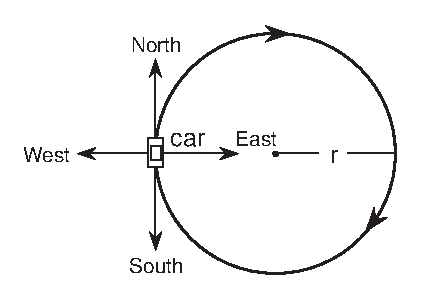
\includegraphics[keepaspectratio,scale=0.66]{June2007-Q04}
    %\begin{tikzpicture}
    %% NOTE: tikz
    %\end{tikzpicture}
    \end{center}
    When the car is in the position shown,
        its acceleration is directed toward the:
    \begin{multicols}{2}
    \begin{choices}
      \correctchoice{east}
        \wrongchoice{west}
        \wrongchoice{south}
        \wrongchoice{north}
    \end{choices}
    \end{multicols}
\end{question}
}

\element{nysed}{
\begin{question}{Jan2007-Q06}
    A ball attached to a string is moved at constant speed in a horizontal circular path.
    A target is located near the path of the ball as shown in the diagram.
    \begin{center}
    \begin{tikzpicture}
        %% Circle
        \draw (0,0) circle (2cm);
        %% Ball and string
        \draw[] (0:0cm) -- (120:2cm) node[anchor=south east] {ball};
        \draw[fill=white] (120:2cm) circle (3pt);
        %% Labels
        \draw[fill] (90:2cm) circle (2pt) node[anchor=south] {$A$};
        \draw[fill] (60:2cm) circle (2pt) node[anchor=south west] {$B$};
        \draw[fill] (-30:2cm) circle (2pt) node[anchor=north west] {$C$};
        \draw[fill] (270:2cm) circle (2pt) node[anchor=north] {$D$};
        %% Target
        %% NOTE: TODO: TARGET NOT finished
        \node[] at (-30:3cm) {target};
        %\draw rectangle
    \end{tikzpicture}
    \end{center}
    At which point along the ball's path should the string be released,
        if the ball is to hit the target?
    \begin{multicols}{4}
    \begin{choices}[o]
        \wrongchoice{$A$}
      \correctchoice{$B$}
        \wrongchoice{$C$}
        \wrongchoice{$D$}
    \end{choices}
    \end{multicols}
\end{question}
}

\element{nysed}{
\begin{question}{June2007-Q08}
    A \SI{0.50}{\kilo\gram} object moves in a horizontal circular path with a radius of \SI{0.25}{\meter} at a constant speed of \SI{4.0}{\meter\per\second}.
    What is the magnitude of the object's acceleration?
    \begin{multicols}{2}
    \begin{choices}
      \correctchoice{\SI{64}{\meter\per\second}}
        \wrongchoice{\SI{8.0}{\meter\per\second}}
        \wrongchoice{\SI{32}{\meter\per\second}}
        \wrongchoice{\SI{16}{\meter\per\second}}
    \end{choices}
    \end{multicols}
\end{question}
}


%% Section Jan2007
%%--------------------


%% Section June2006
%%--------------------
\element{nysed}{
\begin{question}{June2006-Q07}
    The diagram below shows the top view of a \SI{65}{\kilo\gram} student at point $A$ on an amusement park ride.
    The ride spins the student in a horizontal circle of radius \SI{2.5}{\meter}, at a constant speed of \SI{8.6}{\meter\per\second}.
    The floor is lowered and the student remains against the wall without falling to the floor.
    \begin{center}
        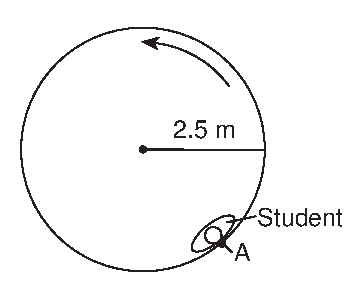
\includegraphics[keepaspectratio,scale=0.8]{June2006-Q07}
    \end{center}
    Which vector best represents the direction of the centripetal acceleration of the student at point $A$?
    \begin{multicols}{2}
    \begin{choices}
        \AMCboxDimensions{down=-0.4cm}
        \correctchoice{
            \begin{tikzpicture}
                \draw[dashed,white!90!black] (0,0) -- (1,1);
                \draw[thick,->] (0.85,0.15) -- (0.15,0.85);
            \end{tikzpicture}
        }
        \wrongchoice{
            \begin{tikzpicture}
                \draw[dashed,white!90!black] (0,0) -- (1,1);
                \draw[thick,->] (0.85,0.85) -- (0.15,0.15);
            \end{tikzpicture}
        }
        \wrongchoice{
            \begin{tikzpicture}
                \draw[dashed,white!90!black] (0,0) -- (1,1);
                \draw[thick,->] (0.15,0.85) -- (0.85,0.15);
            \end{tikzpicture}
        }
        \wrongchoice{
            \begin{tikzpicture}
                \draw[dashed,white!90!black] (0,0) -- (1,1);
                \draw[thick,->] (0.15,0.15) -- (0.85,0.85);
            \end{tikzpicture}
        }
    \end{choices}
    \end{multicols}
\end{question}
}

\element{nysed}{
\begin{question}{June2006-Q08}
    The diagram below shows the top view of a \SI{65}{\kilo\gram} student at point $A$ on an amusement park ride.
    The ride spins the student in a horizontal circle of radius \SI{2.5}{\meter}, at a constant speed of \SI{8.6}{\meter\per\second}.
    The floor is lowered and the student remains against the wall without falling to the floor.
    \begin{center}
        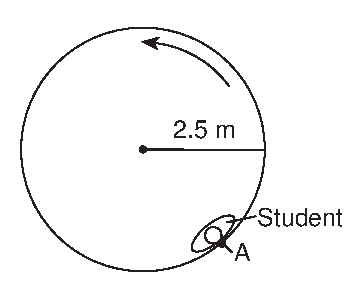
\includegraphics[keepaspectratio,scale=0.8]{June2006-Q07}
    \end{center}
    The magnitude of the centripetal force acting on the student at point $A$ is approximately:
    \begin{multicols}{2}
    \begin{choices}
      \correctchoice{\SI{1.9e3}{\newton}}
        \wrongchoice{\SI{1.2e4}{\newton}}
        \wrongchoice{\SI{2.2e2}{\newton}}
        \wrongchoice{\SI{3.0e1}{\newton}}
    \end{choices}
    \end{multicols}
\end{question}
}


%% Section Jan2006
%%--------------------
\element{nysed}{
\begin{question}{Jan2006-Q14}
    The diagram below shows a \SI{5.0}{\kilo\gram} bucket of water being swung in a horizontal circle of \SI{0.70}{\meter} radius at a constant speed of \SI{2.0}{\meter\per\second}
    \begin{center}
        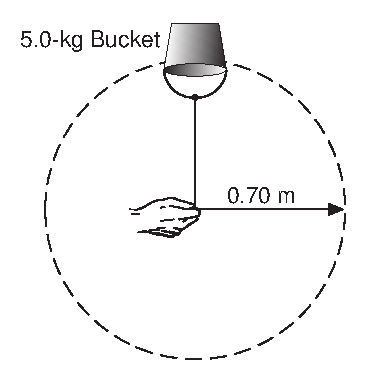
\includegraphics[keepaspectratio,scale=0.75]{Jan2006-Q14}
    \end{center}
    The magnitude of the centripetal force on the buck of water is approximately:
    \begin{multicols}{2}
    \begin{choices}
      \correctchoice{\SI{29}{\newton}}
        \wrongchoice{\SI{14}{\newton}}
        \wrongchoice{\SI{5.7}{\newton}}
        \wrongchoice{\SI{200}{\newton}}
    \end{choices}
    \end{multicols}
\end{question}
}

\element{nysed}{
\begin{question}{Jan2006-Q40}
    In the diagram below, a cart travels clockwise at constant speed in a horizontal circle.
    \begin{center}
        %% NOTE: tikzpicture
        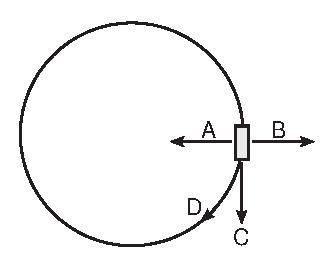
\includegraphics[keepaspectratio,scale=0.8]{Jan2006-Q40}
    \end{center}
    At the position shown in the diagram,
        which arrow indicates the direction of the centripetal acceleration?
    \begin{multicols}{2}
    \begin{choices}
      \correctchoice{$A$}
        \wrongchoice{$B$}
        \wrongchoice{$C$}
        \wrongchoice{$D$}
    \end{choices}
    \end{multicols}
\end{question}
}


%% Section June2005
%%--------------------
\element{nysed}{
\begin{question}{June2005-Q38}
    In the diagram below, $S$ is a point on a car tire rotating at a constant rate.
    \begin{center}
        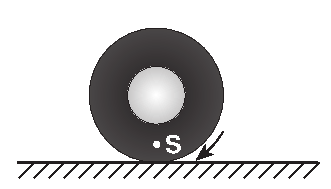
\includegraphics[keepaspectratio,scale=0.8]{June2005-Q38}
    \end{center}
    Which graph best represents the magnitude of the centripetal acceleration of point $S$ as a function of time?
    \begin{multicols}{2}
    \begin{choices}
        \AMCboxDimensions{down=-2.5em}
        \correctchoice{
            \begin{tikzpicture}
                \begin{axis}[
                    axis y line=left,
                    axis x line=bottom,
                    axis line style={->},
                    xlabel={time},
                    xtick=\empty,
                    ylabel={acceleration},
                    ytick=\empty,
                    xmin=0,xmax=11,
                    ymin=0,ymax=11,
                    width=\columnwidth,
                    very thin,
                ]
                \addplot[line width=1pt,domain=0:10]{8};
                \end{axis}
            \end{tikzpicture}
        }
        \wrongchoice{
            \begin{tikzpicture}
                \begin{axis}[
                    axis y line=left,
                    axis x line=bottom,
                    axis line style={->},
                    xlabel={time},
                    xtick=\empty,
                    ylabel={acceleration},
                    ytick=\empty,
                    xmin=0,xmax=11,
                    ymin=0,ymax=11,
                    width=\columnwidth,
                    very thin,
                ]
                \addplot[line width=1pt,domain=0:10]{x};
                \end{axis}
            \end{tikzpicture}
        }
        \wrongchoice{
            \begin{tikzpicture}
                \begin{axis}[
                    axis y line=left,
                    axis x line=bottom,
                    axis line style={->},
                    xlabel={time},
                    xtick=\empty,
                    ylabel={acceleration},
                    ytick=\empty,
                    xmin=0,xmax=11,
                    ymin=0,ymax=11,
                    width=\columnwidth,
                    very thin,
                ]
                \addplot[line width=1pt,domain=0:10]{5/x};
                \end{axis}
            \end{tikzpicture}
        }
        \wrongchoice{
            \begin{tikzpicture}
                \begin{axis}[
                    axis y line=left,
                    axis x line=bottom,
                    axis line style={->},
                    xlabel={time},
                    xtick=\empty,
                    ylabel={acceleration},
                    ytick=\empty,
                    xmin=0,xmax=11,
                    ymin=0,ymax=11,
                    width=\columnwidth,
                    very thin,
                ]
                \addplot[line width=1pt,domain=0:10]{10 - 0.1*(10-x)*(10-x)};
                \end{axis}
            \end{tikzpicture}
        }
    \end{choices}
    \end{multicols}
\end{question}
}

\element{nysed}{
\begin{question}{June2005-Q46}
    A \SI{1.0e3}{\kilo\gram} car travels at a constant speed of \SI{20}{\meter\per\second} around a horizontal circular track.
    Which diagram correctly represents the direction of the car's velocity ($v$) and the direction of the centripetal force ($F_e$) acting on the car at one particular moment?
    \begin{multicols}{2}
    \begin{choices}
        %% NOTE: tikzpicture
      \correctchoice{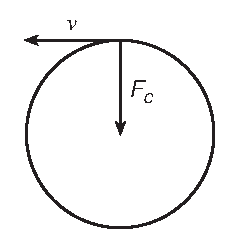
\includegraphics[keepaspectratio,scale=0.66]{June2005-Q46-A}}
        \wrongchoice{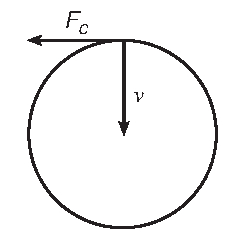
\includegraphics[keepaspectratio,scale=0.66]{June2005-Q46-B}}
        \wrongchoice{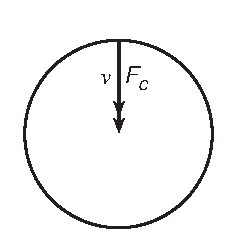
\includegraphics[keepaspectratio,scale=0.66]{June2005-Q46-C}}
        \wrongchoice{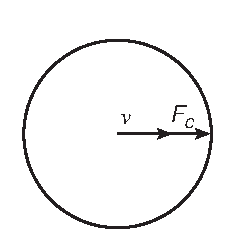
\includegraphics[keepaspectratio,scale=0.66]{June2005-Q46-D}}
    \end{choices}
    \end{multicols}
\end{question}
}


%% Section Jan2005
%%--------------------


%% Section June2004
%%--------------------


%% Section Jan2004
%%--------------------
\element{nysed}{
\begin{question}{Jan2004-Q08}
    $A$ ball of mass $M$ at the end of a string is swung in a horizontal circular path of radius $R$ at constant speed $V$.
    Which combination of changes would require the greatest increase in the centripetal force acting on the ball?
    \begin{choices}
        \wrongchoice{doubling $V$ and doubling $R$}
      \correctchoice{doubling $V$ and halving $R$}
        \wrongchoice{halving $V$ and doubling $R$}
        \wrongchoice{halving $V$ and halving $R$}
    \end{choices}
\end{question}
}


%% Section June2003
%%--------------------
\element{nysed}{
\begin{question}{June2003-Q16}
    A child is riding on merry-go-round.
    As the speed of the merry-go-round is doubled,
        the magnitude of the centripetal force acting on the child:
    \begin{multicols}{2}
    \begin{choices}
      \correctchoice{remains the same}
        \wrongchoice{is doubled}
        \wrongchoice{is halved}
        \wrongchoice{is quadrupled}
    \end{choices}
    \end{multicols}
\end{question}
}


%% Section Jan2003
%%--------------------
\element{nysed}{
\begin{question}{Jan2003-Q09}
    A \SI{2.0e3}{\kilo\gram} car travels at a constant speed of \SI{12}{\meter\per\second} around a circular curve of radius \SI{30}{\meter}.
    What is the magnitude of the centripetal acceleration of the car as it goes around the curve?
    \begin{multicols}{2}
    \begin{choices}
      \correctchoice{\SI{4.8}{\meter\per\second\squared}}
        \wrongchoice{\SI{0.40}{\meter\per\second\squared}}
        \wrongchoice{\SI{800}{\meter\per\second\squared}}
        \wrongchoice{\SI{9600}{\meter\per\second\squared}}
    \end{choices}
    \end{multicols}
\end{question}
}

\element{nysed}{
\begin{question}{Jan2003-Q10}
    A \SI{2.0e3}{\kilo\gram} car travels at a constant speed of \SI{12}{\meter\per\second} around a circular curve of radius \SI{30}{\meter}.
    As the car goes around the curve, the centripetal force is directed:
    \begin{choices}
      \correctchoice{toward the center of the circular curve}
        \wrongchoice{away from the center of the circular curve}
        \wrongchoice{tangent to the curve in the direction of motion}
        \wrongchoice{tangent to the curve opposite the direction of motion}
    \end{choices}
\end{question}
}


%% Section Aug2002
%%--------------------
\element{nysed}{
\begin{question}{Aug2002-Q04}
    The diagram below represents a \SI{0.4}{\kilo\gram} stone attached to a string.
    The stone is moving at a constant speed of \SI{4.0}{\meter\per\second} in a horizontal circle having a radius of \SI{0.8}{\meter}.
    \begin{center}
    %% TODO: NOTE: insert graphic
    \begin{tikzpicture}
        \draw[thick,dashed] (0,0) circle (2cm);
        %\draw[thick,->] (170:2cm) arc (170:170:2cm);
        \draw[thick] (0,0) -- (160:2cm)
            node[pos=0.5,anchor=south west] {$r=\SI{0.80}{\meter}$};
        \draw[fill] (160:2cm) circle (4pt);
        \draw[thick,->] (160:2cm) -- ++(250:0.75cm);
        \node[anchor=south] at (-3.2,0.7) {$m=\SI{0.40}{\kilo\gram}$};
        \node[anchor=north] at (-3.2,0.7) {$v=\SI{4.0}{\meter\per\second}$};
    \end{tikzpicture}
    \end{center}
    The magnitude of the centripetal acceleration of the stone is:
    \begin{multicols}{2}
    \begin{choices}
        \wrongchoice{\SI{0.0}{\meter\per\second\squared}}
        \wrongchoice{\SI{2.0}{\meter\per\second\squared}}
        \wrongchoice{\SI{5.0}{\meter\per\second\squared}}
      \correctchoice{\SI{20}{\meter\per\second\squared}}
    \end{choices}
    \end{multicols}
\end{question}
}


%% Section June2002
%%--------------------
\element{nysed}{
\begin{question}{June2002-Q08}
    The diagram shows a student seated on a rotating circular platform,
    holding a \SI{2.0}{\kilo\gram} block with a spring scale.
    The block is \SI{1.2}{\meter} from the center of the platform.
    The block has a constant speed of \SI{8.0}{\meter\per\second}.
    [Frictional forces on the block are negligible.]
    \begin{center}
        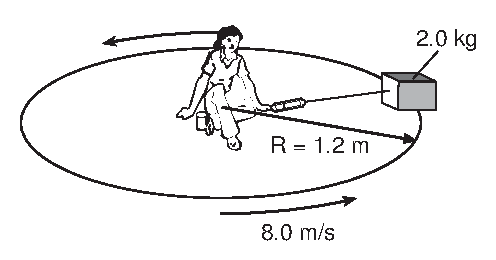
\includegraphics[keepaspectratio,scale=1.0]{June2002-Q08}
    \end{center}
    Which statement best describes the block's movement as the platform rotates?
    \begin{choices}
      \correctchoice{Its velocity is directed tangent to the circular path, with an inward acceleration.}
        \wrongchoice{Its velocity is directed tangent to the circular path, with an outward acceleration.}
        \wrongchoice{Its velocity is directed perpendicular to the circular path, with an inward acceleration.}
        \wrongchoice{Its velocity is directed perpendicular to the circular path, with an outward acceleration.}
    \end{choices}
\end{question}
}

\element{nysed}{
\begin{question}{June2002-Q09}
    The diagram shows a student seated on a rotating circular platform,
    holding a \SI{2.0}{\kilo\gram} block with a spring scale.
    The block is \SI{1.2}{\meter} from the center of the platform.
    The block has a constant speed of \SI{8.0}{\meter\per\second}.
    [Frictional forces on the block are negligible.]
    \begin{center}
        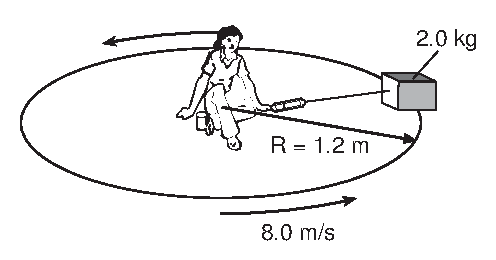
\includegraphics[keepaspectratio,scale=1.0]{June2002-Q08}
    \end{center}
    The reading on the spring scale is approximately:
    \begin{multicols}{2}
    \begin{choices}
        \wrongchoice{\SI{20}{\newton}}
      \correctchoice{\SI{110}{\newton}}
        \wrongchoice{\SI{53}{\newton}}
        \wrongchoice{\SI{130}{\newton}}
    \end{choices}
    \end{multicols}
\end{question}
}


%% Section Jan2002
%%--------------------
\element{nysed}{
\begin{question}{Jan2002-Q59}
    A \SI{60}{\kilo\gram} car travels clockwise in a horizontal circle of radius \SI{10}{\meter} at \SI{5.0}{\meter\per\second}.
    \begin{center}
        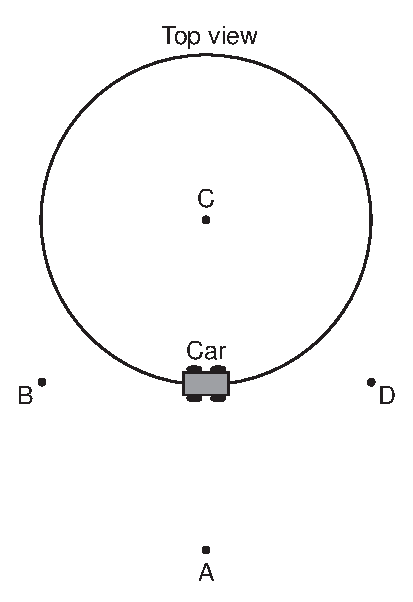
\includegraphics[keepaspectratio,scale=0.8]{Jan2002-Q59}
    \end{center}
    The centripetal acceleration of the car at the position shown is directed toward point:
    \begin{multicols}{2}
    \begin{choices}[o]
        \wrongchoice{$A$}
        \wrongchoice{$B$}
      \correctchoice{$C$}
        \wrongchoice{$D$}
    \end{choices}
    \end{multicols}
\end{question}
}

\element{nysed}{
\begin{question}{Jan2002-Q60}
    A \SI{60}{\kilo\gram} car travels clockwise in a horizontal circle of radius \SI{10}{\meter} at \SI{5.0}{\meter\per\second}.
    \begin{center}
        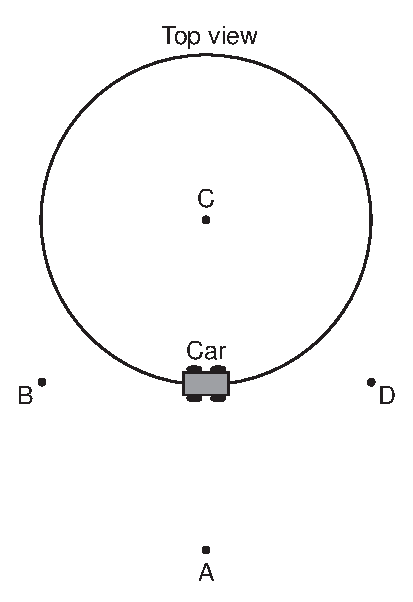
\includegraphics[keepaspectratio,scale=0.8]{Jan2002-Q59}
    \end{center}
    The magnitude of the centripetal force acting on the car is:
    \begin{multicols}{2}
    \begin{choices}
        \wrongchoice{\SI{590}{\newton}}
      \correctchoice{\SI{150}{\newton}}
        \wrongchoice{\SI{30}{\newton}}
        \wrongchoice{\SI{2.5}{\newton}}
    \end{choices}
    \end{multicols}
\end{question}
}


%% Section June2001
%%--------------------
\element{nysed}{
\begin{question}{June2001-Q60}
    A \SI{1200}{\kilo\gram} car traveling at a constant speed of \SI{9.0}{\meter\per\second} turns at an intersection.
    The car follows a horizontal circular path with a radius of \SI{25}{\meter} to point $P$.
    \begin{center}
        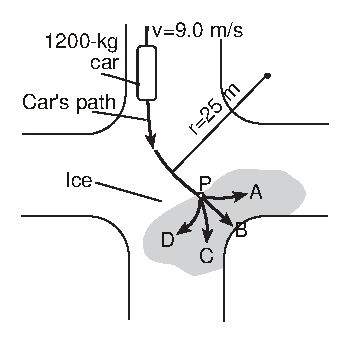
\includegraphics[keepaspectratio,scale=0.9]{June2001-Q60}
    \end{center}
    The magnitude of the centripetal force acting on the car as it travels around the circular path is approximately:
    \begin{multicols}{2}
    \begin{choices}
        \wrongchoice{\SI{1.1e4}{\newton}}
        \wrongchoice{\SI{1.2e4}{\newton}}
      \correctchoice{\SI{3.9e3}{\newton}}
        \wrongchoice{\SI{4.3e2}{\newton}}
    \end{choices}
    \end{multicols}
\end{question}
}

\element{nysed}{
\begin{question}{June2001-Q61}
    A \SI{1200}{\kilo\gram} car traveling at a constant speed of \SI{9.0}{\meter\per\second} turns at an intersection.
    The car follows a horizontal circular path with a radius of \SI{25}{\meter} to point $P$.
    \begin{center}
        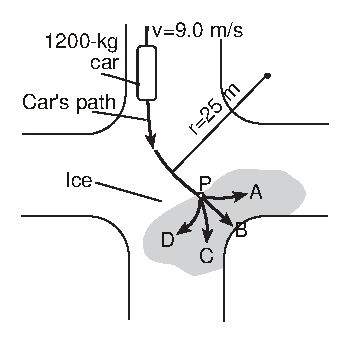
\includegraphics[keepaspectratio,scale=0.9]{June2001-Q60}
    \end{center}
    At point $P$, the car hits an area of ice and loses all frictional force on its tires.
    Which path does the car follow on the ice?
    \begin{multicols}{4}
    \begin{choices}[o]
        \wrongchoice{$A$}
      \correctchoice{$B$}
        \wrongchoice{$C$}
        \wrongchoice{$D$}
    \end{choices}
    \end{multicols}
\end{question}
}

\element{nysed}{
\begin{question}{June2001-Q62}
    An amusement park ride moves a rider at a constant speed of \SI{14}{\meter\per\second} in a horizontal circular path of radius \SI{10}{\meter}.
    What is the rider's centripetal acceleration in terms of $g$,
        the acceleration due to gravity?
    \begin{multicols}{4}
    \begin{choices}
        \wrongchoice{$1g$}
      \correctchoice{$2g$}
        \wrongchoice{$3g$}
        \wrongchoice{$0g$}
    \end{choices}
    \end{multicols}
\end{question}
}


%% Section Jan2001
%%--------------------
\element{nysed}{
\begin{question}{Jan2001-Q56}
    A \SI{1.00e3}{\kilo\gram} car is driven clockwise around a flat circular track of radius \SI{25.0}{\meter}.
    The speed of the car is a constant \SI{5.00}{\meter\per\second}.
    \begin{center}
        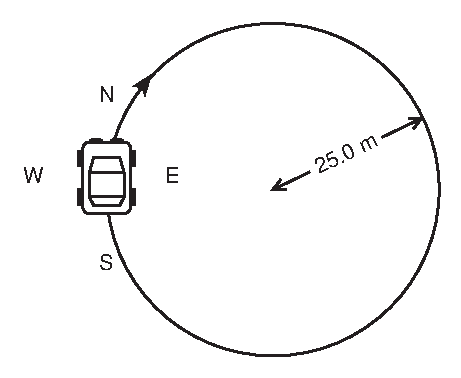
\includegraphics[keepaspectratio,scale=0.8]{Jan2001-Q56}
    \end{center}
    What minimum friction force must exist between the tires and the road to prevent the car from skidding as it rounds the curve?
    \begin{multicols}{2}
    \begin{choices}
        \wrongchoice{\SI{1.25e5}{\newton}}
        \wrongchoice{\SI{9.80e4}{\newton}}
        \wrongchoice{\SI{5.00e3}{\newton}}
      \correctchoice{\SI{1.00e3}{\newton}}
    \end{choices}
    \end{multicols}
\end{question}
}

\element{nysed}{
\begin{question}{Jan2001-Q57}
    A \SI{1.00e3}{\kilo\gram} car is driven clockwise around a flat circular track of radius \SI{25.0}{\meter}.
    The speed of the car is a constant \SI{5.00}{\meter\per\second}.
    \begin{center}
        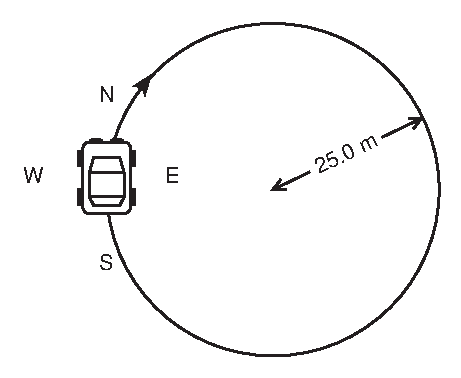
\includegraphics[keepaspectratio,scale=0.8]{Jan2001-Q56}
    \end{center}
    If the circular track were to suddenly become frictionless at the instant shown in the diagram,
        the car's direction of travel would be:
    \begin{multicols}{2}
    \begin{choices}
        \wrongchoice{toward E}
      \correctchoice{toward N}
        \wrongchoice{toward W}
        \wrongchoice{a clockwise spiral}
    \end{choices}
    \end{multicols}
\end{question}
}

\element{nysed}{
\begin{question}{Jan2001-Q57}
    A \SI{1.00e3}{\kilo\gram} car is driven clockwise around a flat circular track of radius \SI{25.0}{\meter}.
    The speed of the car is a constant \SI{5.00}{\meter\per\second}.
    \begin{center}
        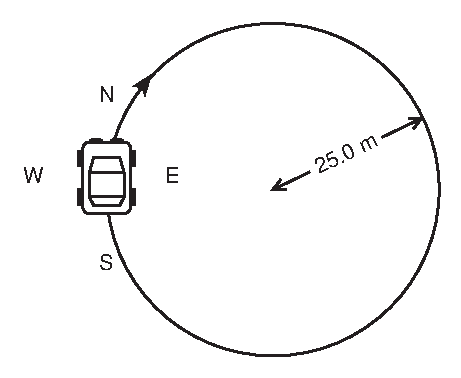
\includegraphics[keepaspectratio,scale=0.8]{Jan2001-Q56}
    \end{center}
    If the circular track were to suddenly become frictionless at the instant shown in the diagram,
        the car's direction of travel would be:
    \begin{multicols}{2}
    \begin{choices}
        \wrongchoice{toward E}
      \correctchoice{toward N}
        \wrongchoice{toward W}
        \wrongchoice{a clockwise spiral}
    \end{choices}
    \end{multicols}
\end{question}
}

\element{nysed}{
\begin{question}{Jan2001-Q58}
    A \SI{1.00e3}{\kilo\gram} car is driven clockwise around a flat circular track of radius \SI{25.0}{\meter}.
    The speed of the car is a constant \SI{5.00}{\meter\per\second}.
    \begin{center}
        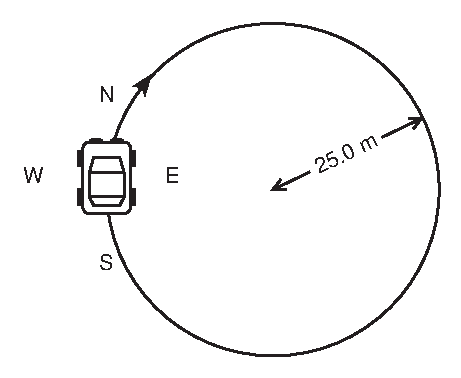
\includegraphics[keepaspectratio,scale=0.8]{Jan2001-Q56}
    \end{center}
    At the instant shown in the diagram,
        the car's centripetal acceleration is directed:
    \begin{multicols}{2}
    \begin{choices}
      \correctchoice{toward E}
        \wrongchoice{toward N}
        \wrongchoice{toward W}
        \wrongchoice{clockwise}
    \end{choices}
    \end{multicols}
\end{question}
}

\element{nysed}{
\begin{question}{Jan2001-Q59}
    A \SI{1.00e3}{\kilo\gram} car is driven clockwise around a flat circular track of radius \SI{25.0}{\meter}.
    The speed of the car is a constant \SI{5.00}{\meter\per\second}.
    \begin{center}
        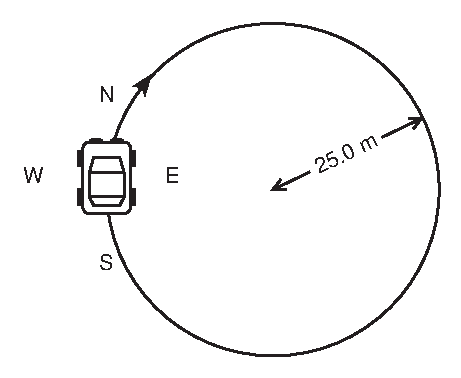
\includegraphics[keepaspectratio,scale=0.8]{Jan2001-Q56}
    \end{center}
    Which factor, when doubled, would produce the greatest change in the centripetal force acting on the car?
    \begin{multicols}{2}
    \begin{choices}
        \wrongchoice{mass of the car}
        \wrongchoice{radius of the track}
      \correctchoice{velocity of the car}
        \wrongchoice{weight of the car}
    \end{choices}
    \end{multicols}
\end{question}
}


%% Section June2000
%%--------------------
\element{nysed}{
\begin{question}{June2000-Q60}
    As a cart travels around a horizontal circular track,
        the cart \emph{must} undergo a change in:
    \begin{multicols}{2}
    \begin{choices}
      \correctchoice{velocity}
        \wrongchoice{inertia}
        \wrongchoice{speed}
        \wrongchoice{weight}
    \end{choices}
    \end{multicols}
\end{question}
}

\element{nysed}{
\begin{question}{June2000-Q64}
    A ball attached to a string is whirled at a constant speed of \SI{2.0}{\meter\per\second} in a horizontal circle of radius \SI{0.50}{\meter}.
    What is the magnitude of the ball's centripetal acceleration?
    \begin{multicols}{2}
    \begin{choices}
        \wrongchoice{\SI{1.0}{\meter\per\second\squared}}
        \wrongchoice{\SI{2.0}{\meter\per\second\squared}}
      \correctchoice{\SI{8.0}{\meter\per\second\squared}}
        \wrongchoice{\SI{4.0}{\meter\per\second\squared}}
    \end{choices}
    \end{multicols}
\end{question}
}


%% Section June1999
%%--------------------
\newcommand{\JuneNineteenNinetyNineQSixtyThree}{
\begin{tikzpicture}
    %% Circle
    \draw[dashed] (0,0) circle (2cm);
    %% Arrows
    \foreach \x in {45,135,225,315} \draw[black,thick,->] (\x:2) arc(\x:{\x-5}:2);
    \draw[thick,-latex] (0,0) -- (30:2) node[pos=0.4,anchor=north west] {\SI{2.0}{\meter}};
    \node[anchor=north] at (0,-2) {top view};
    %% options
    \fill (-2,0) ++(90:1.5) circle (2pt) node[anchor=south] {$B$};
    \fill (-2,0) ++(180:1) circle (2pt) node[anchor=south] {$C$};
    \fill (-2,0) ++(270:1.5) circle (2pt) node[anchor=north] {$D$};
    \fill (-2,0) ++(0:1) circle (2pt) node[anchor=south] {$A$};
    %% Rock and directions
    \fill (180:2) circle (1ex);
    \node[pin={[text width=4em,pin edge={latex-,shorten <=1mm}]225:{\SI{7.0}{\kilo\gram} hammer}}] at (180:2) {};
    \draw[very thick,->] (0,0) -- (180:2);
\end{tikzpicture}
}

\element{nysed}{
\begin{question}{June1999-Q63}
    An athlete in a hammer-throw event swings a \SI{7.0}{\kilo\gram} hammer in a horizontal circle at a constant speed of \SI{12}{\meter\per\second}.
    The radius of the hammer's path is \SI{2.0}{\meter}.
    \begin{center}
        \JuneNineteenNinetyNineQSixtyThree
    \end{center}
    At the position shown,
        the centripetal force acting on the hammer is directed toward point:
    \begin{multicols}{4}
    \begin{choices}[o]
      \correctchoice{$A$}
        \wrongchoice{$B$}
        \wrongchoice{$C$}
        \wrongchoice{$D$}
    \end{choices}
    \end{multicols}
\end{question}
}

\element{nysed}{
\begin{question}{June1999-Q64}
    An athlete in a hammer-throw event swings a \SI{7.0}{\kilo\gram} hammer in a horizontal circle at a constant speed of \SI{12}{\meter\per\second}.
    The radius of the hammer's path is \SI{2.0}{\meter}.
    \begin{center}
        \JuneNineteenNinetyNineQSixtyThree
    \end{center}
    What is the magnitude of the centripetal acceleration of the hammer?
    \begin{multicols}{2}
    \begin{choices}
        \wrongchoice{\SI{6.0}{\meter\per\second\squared}}
        \wrongchoice{\SI{24}{\meter\per\second\squared}}
      \correctchoice{\SI{72}{\meter\per\second\squared}}
        \wrongchoice{\SI{500}{\meter\per\second\squared}}
    \end{choices}
    \end{multicols}
\end{question}
}

\element{nysed}{
\begin{question}{June1999-Q66}
    An athlete in a hammer-throw event swings a \SI{7.0}{\kilo\gram} hammer in a horizontal circle at a constant speed of \SI{12}{\meter\per\second}.
    The radius of the hammer's path is \SI{2.0}{\meter}.
    \begin{center}
        \JuneNineteenNinetyNineQSixtyThree
    \end{center}
    If the hammer is released at the position shown,
        it will travel toward point:
    \begin{multicols}{4}
    \begin{choices}[o]
        \wrongchoice{$A$}
      \correctchoice{$B$}
        \wrongchoice{$C$}
        \wrongchoice{$D$}
    \end{choices}
    \end{multicols}
\end{question}
}


%% Section June1998
%%--------------------

%% NOTE: June1998-Q58 requires graphic, tikz?
%% NOTE: June1998-Q59 same as Q58
%% NOTE: June1998-Q60 same as Q58
\newcommand{\JuneNineteenNinetyNineQFiftyEight}{
\begin{tikzpicture}
    %% path
\end{tikzpicture}
}

\element{nysed}{
\begin{question}{June1998-Q59}
    The diagram below shows a \SI{2.0}{\kilo\gram} cart traveling at a constant speed in a horizontal circle of radius \SI{3.0}{\meter}.
    The magnitude of the centripetal force of the cart is \SI{24}{\newton}.
    \begin{center}
        \JuneNineteenNinetyNineQFiftyEight
    \end{center}
    In the position shown, the acceleration of the cart is:
    \begin{choices}
        \wrongchoice{\SI{8.0}{\meter\per\second\squared} directed toward point $A$}
        \wrongchoice{\SI{8.0}{\meter\per\second\squared} directed toward point $D$}
        \wrongchoice{\SI{12.0}{\meter\per\second\squared} directed toward point $A$}
        \wrongchoice{\SI{12.0}{\meter\per\second\squared} directed toward point $D$}
    \end{choices}
\end{question}
}

\element{nysed}{
\begin{question}{June1998-Q60}
    The diagram below shows a \SI{2.0}{\kilo\gram} cart traveling at a constant speed in a horizontal circle of radius \SI{3.0}{\meter}.
    The magnitude of the centripetal force of the cart is \SI{24}{\newton}.
    \begin{center}
        \JuneNineteenNinetyNineQFiftyEight
    \end{center}
    Which statement correctly describes the direction of the cart's velocity and centripetal force in the position shown?
    \begin{choices}
        \wrongchoice{velocity is directed toward point $B$, and the centripetal force is directed toward point $A$}
        \wrongchoice{velocity is directed toward point $B$, and the centripetal force is directed toward point $D$}
        \wrongchoice{velocity is directed toward point $C$, and the centripetal force is directed toward point $A$}
        \wrongchoice{velocity is directed toward point $C$, and the centripetal force is directed toward point $D$}
    \end{choices}
\end{question}
}

\element{nysed}{
\begin{question}{June1998-Q61}
    The diagram below shows a \SI{2.0}{\kilo\gram} cart traveling at a constant speed in a horizontal circle of radius \SI{3.0}{\meter}.
    The magnitude of the centripetal force of the cart is \SI{24}{\newton}.
    \begin{center}
        \JuneNineteenNinetyNineQFiftyEight
    \end{center}
    What is the speed of the cart?
    \begin{multicols}{2}
    \begin{choices}
        \wrongchoice{\SI{6.0}{\meter\per\second}}
        \wrongchoice{\SI{16}{\meter\per\second}}
        \wrongchoice{\SI{36}{\meter\per\second}}
        \wrongchoice{\SI{4.0}{\meter\per\second}}
    \end{choices}
    \end{multicols}
\end{question}
}


%% Section June1997
%%--------------------
\element{nysed}{
\begin{question}{June1997-Q07}
    A ball rolls through a hollow semicircular tube lying flat on a horizontal tabletop.
    Which diagram shows the path of the ball after emerging from the tube,
        as viewed from above?
    \begin{multicols}{2}
    \begin{choices}
        \AMCboxDimensions{down=-1cm}
        \wrongchoice{
            \begin{tikzpicture}
                %% table top
                \draw[dashed,white!60!black] (-1.5,-2.5) rectangle (1.5,1.5);
                \node[anchor=south] at (0,-2.5) {Tabletop};
                %% loop
                \draw (0,1.2) arc (90:270:1.2) arc(270:90:0.05 and 0.1) arc(270:90:1.0) arc(270:90:0.05 and 0.1) -- cycle;
                \draw (0,-1.1) circle (0.05 and 0.1);
                \draw (0,+1.1) circle (0.05 and 0.1);
                %% ball and vector
                \fill (0.05,-1.1) circle (0.04 and 0.08);
                \draw[thick,->] (0,-1.1) arc(270:360:1.1);
            \end{tikzpicture}
        }
        \wrongchoice{
            \begin{tikzpicture}
                %% table top
                \draw[dashed,white!60!black] (-1.5,-2.5) rectangle (1.5,1.5);
                \node[anchor=south] at (0,-2.5) {Tabletop};
                %% loop
                \draw (0,1.2) arc (90:270:1.2) arc(270:90:0.05 and 0.1) arc(270:90:1.0) arc(270:90:0.05 and 0.1) -- cycle;
                \draw (0,-1.1) circle (0.05 and 0.1);
                \draw (0,+1.1) circle (0.05 and 0.1);
                %% ball and vector
                \fill (0.05,-1.1) circle (0.04 and 0.08);
                \draw[thick,->] (0,-1.1) arc(90:0:1.1);
            \end{tikzpicture}
        }
        \wrongchoice{
            \begin{tikzpicture}
                %% table top
                \draw[dashed,white!60!black] (-1.5,-2.5) rectangle (1.5,1.5);
                \node[anchor=south] at (0,-2.5) {Tabletop};
                %% loop
                \draw (0,1.2) arc (90:270:1.2) arc(270:90:0.05 and 0.1) arc(270:90:1.0) arc(270:90:0.05 and 0.1) -- cycle;
                \draw (0,-1.1) circle (0.05 and 0.1);
                \draw (0,+1.1) circle (0.05 and 0.1);
                %% ball and vector
                \fill (0.05,-1.1) circle (0.04 and 0.08);
                \draw[thick,->] (0,-1.1) -- ++(270:0.8);
            \end{tikzpicture}
        }
        %% Newton's first law
        \correctchoice{
            \begin{tikzpicture}
                %% table top
                \draw[dashed,white!60!black] (-1.5,-2.5) rectangle (1.5,1.5);
                \node[anchor=south] at (0,-2.5) {Tabletop};
                %% loop
                \draw (0,1.2) arc (90:270:1.2) arc(270:90:0.05 and 0.1) arc(270:90:1.0) arc(270:90:0.05 and 0.1) -- cycle;
                \draw (0,-1.1) circle (0.05 and 0.1);
                \draw (0,+1.1) circle (0.05 and 0.1);
                %% ball and vector
                \fill (0.05,-1.1) circle (0.04 and 0.08);
                \draw[thick,->] (0,-1.1) -- ++(0:1);
            \end{tikzpicture}
        }
    \end{choices}
    \end{multicols}
\end{question}
}

%% NOTE: Q58 to Q60 uses common graphic
%% NOTE: June1997-Q58 requires graphics
%% NOTE: June1997-Q59 requires graphics
%% NOTE: June1997-Q60 requires graphics


%% Section June1996
%%--------------------
\newcommand{\JuneOneNineNineSixQFiftyNine}{
\begin{tikzpicture}
    %% path
    \draw[dashed] (0,0) circle (3cm and 0.75cm);
    \draw[thick,->] (0,0) -- (180:3) node[pos=0.5,anchor=south] {string};
    %% arrows
    \foreach \x in {45,135,225,315}
        \draw[thick,-latex] ({3*cos(\x)},{0.75*sin(\x)}) arc(\x:{\x-10}:3 and 0.75);
    %% ball
    \fill (180:3) circle (2pt) node[anchor=east,xshift=-2pt] {ball};
    %% hand
    \draw[thick,->] (0,-1) -- (0,0) node[pos=0,anchor=north] {hand};
\end{tikzpicture}
}

\element{nysed}{
\begin{question}{June1996-Q59}
    The diagram shows a student spinning a \SI{0.10}{\kilo\gram} ball at the end of a \SI{0.50}{\meter} string in a horizontal circle at a constant speed of \SI{10}{\meter\per\second}.
    [Neglect air resistance.]
    \begin{center}
        %% NOTE: tikz?
        \JuneOneNineNineSixQFiftyNine
    \end{center}
    If the magnitude of the force applied to the string by the student's hand is increased,
        the magnitude of the acceleration of the ball in its circular path will:
    \begin{choices}
        \wrongchoice{decrease}
      \correctchoice{increase}
        \wrongchoice{remain the same}
    \end{choices}
\end{question}
}

\element{nysed}{
\begin{question}{June1996-Q60}
    The diagram shows a student spinning a \SI{0.10}{\kilo\gram} ball at the end of a \SI{0.50}{\meter} string in a horizontal circle at a constant speed of \SI{10}{\meter\per\second}.
    [Neglect air resistance.]
    \begin{center}
        \JuneOneNineNineSixQFiftyNine
    \end{center}
    The magnitude of the centripetal force required to keep the ball in this circular path is:
    \begin{multicols}{2}
    \begin{choices}
        \wrongchoice{\SI{5.0}{\newton}}
        \wrongchoice{\SI{10}{\newton}}
      \correctchoice{\SI{20}{\newton}}
        \wrongchoice{\SI{200}{\newton}}
    \end{choices}
    \end{multicols}
\end{question}
}

\element{nysed}{
\begin{question}{June1996-Q61}
    The diagram shows a student spinning a \SI{0.10}{\kilo\gram} ball at the end of a \SI{0.50}{\meter} string in a horizontal circle at a constant speed of \SI{10}{\meter\per\second}.
    [Neglect air resistance.]
    \begin{center}
        \JuneOneNineNineSixQFiftyNine
    \end{center}
    Which is the best description of the force keeping the ball in the circular path?
    \begin{choices}
      \correctchoice{perpendicular to the circle and directed toward the center of the circle}
        \wrongchoice{perpendicular to the circle and directed away from the center of the circle}
        \wrongchoice{tangent to the circle and directed in the same direction that the ball is moving}
        \wrongchoice{tangent to the circle and directed opposite to the direction that the ball is moving}
    \end{choices}
\end{question}
}

\element{nysed}{
\begin{question}{June1996-Q62}
    A convertible car with its top down is traveling at constant speed around a circular track,
        as shown in the diagram below.
    \begin{center}
    \begin{tikzpicture}
        %% track
        \draw (0,0) circle (2cm);
        %% car
        \draw[very thick,->] (0,-2) arc (270:300:2);
        \draw[fill=white!90!black] (-0.25,-1.9) rectangle (0.25,-2.1);
        \node[anchor=south] at (0,-1.9) {car};
        %% Options
        \fill (2,0) circle (2pt) node[anchor=west] {$A$};
        \fill (2,2) circle (2pt) node[anchor=west] {$C$};
        \fill (0,2) circle (2pt) node[anchor=north] {$B$};
        \fill (3,0) circle (2pt) node[anchor=south] {$D$};
    \end{tikzpicture}
    \end{center}
    When the car is at point $I$, if a passenger in the car throws a ball straight up,
        the ball could land at point:
    \begin{multicols}{4}
    \begin{choices}[o]
        \wrongchoice{$A$}
        \wrongchoice{$B$}
      \correctchoice{$C$}
        \wrongchoice{$D$}
    \end{choices}
    \end{multicols}
\end{question}
}


%% Section June1995
%%--------------------
\newcommand{\nysedJuneNineteenNinetyFiveQFiftyNine}{
\begin{tikzpicture}
    %% clockwise path
    \draw[dashed] (0,0) circle (2cm);
    \draw[thick,-latex] (0,0) -- (135:2) node[pos=0.5,anchor=south,rotate=-45] {\SI{2.0}{\meter}};
    \foreach \x in {100,220,340}
        \draw[thick,-latex] (\x:2) arc(\x:{\x-2}:2);
    %% Cart
    \node[minimum height=1ex,minimum width=0.66ex,draw,fill] (C) at (2,0) {};
    \node[anchor=west] at (C.east) {Cart};
    %% options
    \fill (0,0) circle (2pt) node[anchor=south west] {$Q$};
    \fill (4,0) circle (2pt) node[anchor=south west] {$R$};
    \fill (2,-2) circle (2pt) node[anchor=south west] {$S$};
    \fill (0,-2) circle (2pt) node[anchor=north west] {$P$};
\end{tikzpicture}
}

\element{nysed}{
\begin{question}{June1995-Q59}
    The diagram shows a \SI{5.0}{\kilo\gram} cart traveling clockwise in a horizontal circle of radius \SI{2.0}{\meter} at a constant speed of \SI{4.0}{\meter\per\second}.
    \begin{center}
        \nysedJuneNineteenNinetyFiveQFiftyNine
    \end{center}
    %% start question
    At the position show, the velocity of the cart is directed toward point?
    \begin{multicols}{4}
    \begin{choices}
        \wrongchoice{$P$}
        \wrongchoice{$Q$}
        \wrongchoice{$R$}
      \correctchoice{$S$}
    \end{choices}
    \end{multicols}
\end{question}
}

\element{nysed}{
\begin{question}{June1995-Q60}
    The diagram shows a \SI{5.0}{\kilo\gram} cart traveling clockwise in a horizontal circle of radius \SI{2.0}{\meter} at a constant speed of \SI{4.0}{\meter\per\second}.
    \begin{center}
        \nysedJuneNineteenNinetyFiveQFiftyNine
    \end{center}
    %% start question
    At the position show, the centripetal acceleration of the cart is directed toward point:
    \begin{multicols}{4}
    \begin{choices}
        \wrongchoice{$P$}
      \correctchoice{$Q$}
        \wrongchoice{$R$}
        \wrongchoice{$S$}
    \end{choices}
    \end{multicols}
\end{question}
}

\element{nysed}{
\begin{question}{June1995-Q61}
    The diagram shows a \SI{5.0}{\kilo\gram} cart traveling clockwise in a horizontal circle of radius \SI{2.0}{\meter} at a constant speed of \SI{4.0}{\meter\per\second}.
    \begin{center}
        \nysedJuneNineteenNinetyFiveQFiftyNine
    \end{center}
    %% start question
    If the mass of the cart was doubled,
        the magnitude of the centripetal acceleration of the cart would be:
    \begin{multicols}{2}
    \begin{choices}
      \correctchoice{unchanged}
        \wrongchoice{doubled}
        \wrongchoice{halved}
        \wrongchoice{quadrupled}
    \end{choices}
    \end{multicols}
\end{question}
}

\element{nysed}{
\begin{question}{June1995-Q62}
    The diagram shows a \SI{5.0}{\kilo\gram} cart traveling clockwise in a horizontal circle of radius \SI{2.0}{\meter} at a constant speed of \SI{4.0}{\meter\per\second}.
    \begin{center}
        \nysedJuneNineteenNinetyFiveQFiftyNine
    \end{center}
    %% start question
    What is the magnitude of the centripetal force acting on the cart?
    \begin{multicols}{2}
    \begin{choices}
        \wrongchoice{\SI{8.0}{\newton}}
        \wrongchoice{\SI{20}{\newton}}
      \correctchoice{\SI{40}{\newton}}
        \wrongchoice{\SI{50}{\newton}}
    \end{choices}
    \end{multicols}
\end{question}
}


%% Section June1994
%%--------------------


%% Section June1989
%%--------------------
\element{nysed}{
\begin{question}{June1989-Q62}
    Two masses, $A$ and $B$, move in circular path as shown in the diagram.
    \begin{center}
    \begin{tikzpicture}[scale=1.33]
        \fill (0,0) circle (2pt);
        %% A loop
        \fill (90:1.5) circle (2pt) node[anchor=south] {$A$};
        \draw[thick,-latex] (0,0) -- (45:1.5) node[pos=0.5,anchor=center,fill=white,rotate=-45] {\SI{1}{\meter}};
        \draw[very thick,-latex] (1.5,0) arc(0:120:1.5) node[pos=0.375,anchor=south,rotate=-45] {$v=\SI{2}{\meter\per\second}$};
        %% B loop
        \fill (140:3) circle (2pt) node[anchor=south east] {$B$};
        \draw[thick,-latex] (0,0) -- (135:3) node[pos=0.75,anchor=center,fill=white,rotate=45] {\SI{2}{\meter}};
        \draw[very thick,-latex] (45:3) arc(45:160:3);
        \node[anchor=south] at (0,3) {$v=\SI{2}{\meter\per\second}$};
    \end{tikzpicture}
    \end{center}
    The centripetal acceleration of mass $A$,
        compared to that of mass $B$, is:
    \begin{choices}
        \wrongchoice{the same}
      \correctchoice{twice as great}
        \wrongchoice{one-half as great}
        \wrongchoice{four times as great}
    \end{choices}
\end{question}
}

\element{nysed}{
\begin{question}{June1989-Q65}
    The diagram below shows an object traveling clockwise in a horizontal,
        circular path at constant speed.
    \begin{center}
    \begin{tikzpicture}
        \fill (0,0) circle (1.5pt);
        %% path
        \draw (0,0) circle (2cm);
        \draw[thick,->] (135:2.5) arc(135:80:2.5);
        \path[postaction={decoration={text along path, text={clockwise},text align=center},decorate}] (135:2.7) arc(135:80:2.7);
        \path[postaction={decoration={text along path, text={motion},text align=center},decorate}] (135:2.1) arc(135:80:2.1);
        %% object
        \draw[fill=white!60!black] (2,0) circle (5pt) node[anchor=west,xshift=5pt] {object};
    \end{tikzpicture}
    \end{center}
    Which arrow best shows the direction of the centripetal acceleration of the object at the instant shown?
    \begin{multicols}{2}
    \begin{choices}
        \AMCboxDimensions{down=-0.8cm}
        \correctchoice{
            \begin{tikzpicture}[scale=2]
                \draw[dashed,white!60!black] (0,0) rectangle (1,1);
                \draw[thick,->] (1,0.5) -- (0,0.5);
            \end{tikzpicture}
        }
        \wrongchoice{
            \begin{tikzpicture}[scale=2]
                \draw[dashed,white!60!black] (0,0) rectangle (1,1);
                \draw[thick,->] (0,0.5) -- (1,0.5);
            \end{tikzpicture}
        }
        \wrongchoice{
            \begin{tikzpicture}[scale=2]
                \draw[dashed,white!60!black] (0,0) rectangle (1,1);
                \draw[thick,->] (0.5,1) -- (0.5,0);
            \end{tikzpicture}
        }
        \wrongchoice{
            \begin{tikzpicture}[scale=2]
                \draw[dashed,white!60!black] (0,0) rectangle (1,1);
                \draw[thick,->] (0.5,0) -- (0.5,1);
            \end{tikzpicture}
        }
    \end{choices}
    \end{multicols}
\end{question}
}


\endinput



%
%% Waves Questions used on the
%% NYSED Physics Regents Examination
%%--------------------------------------------------

%% this section contains 160 problems


%% Section June2015
%%--------------------
\element{nysed}{
\begin{question}{June2015-Q24}
    A student produces a wave in a long spring by vibrating its end.
    As the frequency of the vibration is doubled,
        the wavelength in the spring is:
    \begin{multicols}{2}
    \begin{choices}
        \wrongchoice{quartered}
      \correctchoice{halved}
        \wrongchoice{unchanged}
        \wrongchoice{doubled}
    \end{choices}
    \end{multicols}
\end{question}
}

\element{nysed}{
\begin{question}{June2015-Q25}
    Which two points on the wave shown in the diagram below are in phase with each other?
    \begin{center}
    \begin{tikzpicture}[x=0.05\textwidth]
        %% Graph
        \draw[domain=0:5*pi,smooth,line width=1pt] plot (\x, {sin(\x r)});
        %% Labels
        \draw[fill] (1.57,1) circle (2pt) node[anchor=south] {$A$};
        \draw[fill] (3.14,0) circle (2pt) node[anchor=south west] {$B$};
        \draw[fill] (6.28,0) circle (2pt) node[anchor=south east] {$C$};
        \draw[fill] (9.42,0) circle (2pt) node[anchor=south west] {$D$};
        \draw[fill] (11.0,-1) circle (2pt) node[anchor=south] {$E$};
    \end{tikzpicture}
    \end{center}
    \begin{multicols}{2}
    \begin{choices}
        \wrongchoice{$A$ and $B$}
        \wrongchoice{$A$ and $E$}
        \wrongchoice{$B$ and $C$}
      \correctchoice{$B$ and $D$}
    \end{choices}
    \end{multicols}
\end{question}
}

\element{nysed}{
\begin{question}{June2015-Q26}
    As a longitudinal wave moves through a medium,
        the particles of the medium:
    \begin{choices}
      \correctchoice{vibrate parallel to the direction of the wave's propagation.}
        \wrongchoice{vibrate perpendicular to the direction of the wave's propagation.}
        \wrongchoice{are transferred in the direction of the wave’s motion, only.}
        \wrongchoice{are stationary.}
    \end{choices}
\end{question}
}

\element{nysed}{
\begin{question}{June2015-Q27}
    Wind blowing across suspended power lines may cause the power lines to vibrate at their natural frequency.
    This often produces audible sound waves.
    This phenomenon, often called an Aeolian harp,
        is an example of:
    \begin{multicols}{2}
    \begin{choices}
        \wrongchoice{diffraction}
        \wrongchoice{the Doppler effect}
        \wrongchoice{refraction}
      \correctchoice{resonance}
    \end{choices}
    \end{multicols}
\end{question}
}

\element{nysed}{
\begin{question}{June2015-Q35}
    Two pulses approach each other in the same medium.
    The diagram below represents the displacements caused by each pulse.
    \begin{center}
    \begin{tikzpicture}
        \draw[thick] (-3,0) -- (-2,0) -- (-2,-1) -- (-1,-1) -- (-1,0) --
                     (+1,0) -- (+1,1) -- (+2,1.5) -- (+2,0) -- (+3,0);
        \draw[thick,->] (-2,-1.2) -- (-1,-1.2);
        \draw[thick,->] (+2,-1.2) -- (+1,-1.2);
    \end{tikzpicture}
    \end{center}
    Which diagram best represents the resultant displacement of the medium as the pulses pass through each other?
    \begin{multicols}{2}
    \begin{choices}
        \AMCboxDimensions{down=-0.5cm}
        \wrongchoice{
            \begin{tikzpicture}
                \draw[white] (-1.5,-0.5) rectangle (1.5,3.0);
                \draw[thick] (-1.5,0) -- (1.5,0);
            \end{tikzpicture}
        }
        \correctchoice{
            \begin{tikzpicture}
                \draw[white] (-1.5,-0.5) rectangle (1.5,3.0);
                \draw[thick] (-1.5,0) -- (-0.5,0) -- (0.5,0.5) -- (0.5,0) --  (1.5,0);
            \end{tikzpicture}
        }
        \wrongchoice{
            \begin{tikzpicture}
                \draw[white] (-1.5,-0.5) rectangle (1.5,3.0);
                \draw[thick] (-1.5,0) -- (-0.5,0) -- (-0.5,2.0) -- (0.5,2.5) -- (0.5,0) --  (1.5,0);
            \end{tikzpicture}
        }
        \wrongchoice{
            \begin{tikzpicture}
                \draw[white] (-1.5,-0.5) rectangle (1.5,3.0);
                \draw[thick] (-1.5,0) -- (-0.5,0) -- (0.5,-0.5) -- (0.5,0) --  (1.5,0);
            \end{tikzpicture}
        }
    \end{choices}
    \end{multicols}
\end{question}
}

\element{nysed}{
\begin{question}{June2015-Q49}
    The diagram below shows waves $A$ and $B$ in the same medium.
    %Wave $A$ and $B$ are represented as a dashed and solid line.
    \begin{center}
    \begin{tikzpicture}[x=0.045\textwidth,yscale=0.8]
        %% Graph
        \draw[domain=0:6*pi,smooth,line width=1pt] plot (\x, {2.0*sin(\x r)});
        \draw[domain=0:6*pi,dashed,smooth,line width=1pt] plot (\x, {sin(0.5*\x r)});
        %% Labels
        \node[anchor=south west] at (8.7,{2.0*sin(8.7 r)})  {$B$};
        \node[anchor=south west] at (18,{sin(0.5*18 r)})  {$A$};
    \end{tikzpicture}
    \end{center}
    Compared to wave $A$, wave $B$ has:
    \begin{choices}
        \wrongchoice{twice the amplitude and twice the wavelength.}
      \correctchoice{twice the amplitude and half the wavelength.}
        \wrongchoice{the same amplitude and half the wavelength.}
        \wrongchoice{half the amplitude and the same wavelength.}
    \end{choices}
\end{question}
}


%% Section June2014
%%--------------------
\element{nysed}{
\begin{question}{June2014-Q17}
    Transverse waves are to radio waves as longitudinal waves are to:
    \begin{multicols}{2}
    \begin{choices}
      \correctchoice{sound waves}
        \wrongchoice{light waves}
        \wrongchoice{microwaves}
        \wrongchoice{ultraviolet waves}
    \end{choices}
    \end{multicols}
\end{question}
}

\element{nysed}{
\begin{question}{June2014-Q25}
    The diagram below represents two identical pulses approaching each other in a uniform medium.
    \begin{center}
    \begin{tikzpicture}
        \begin{axis}[
            clip=false,
            axis y line=left,
            axis x line=center,
            axis line style={->},
            xlabel=\empty,
            xtick=\empty,
            ylabel={displacement},
            y unit=\si{\centi\meter},
            ytick={-6,-3,0,3,6},
            xmin=0,xmax=10,
            ymin=-7,ymax=7,
            grid=major,
            width=0.95\columnwidth,
            height=0.618\columnwidth,
            very thin,
        ]
        \addplot[very thick,domain=0:2]{0};
        \addplot[very thick,domain=4:6]{0};
        \addplot[very thick,domain=8:10]{0};
        %% Waves
        \addplot[very thick,domain=2:4]{-3*(x-2)*(x-4)};
        \addplot[very thick,domain=6:8]{-3*(x-6)*(x-8)};
        %% Arrows
        \draw[very thick,->] (axis cs:2,4) -- (axis cs:4,4);
        \draw[very thick,->] (axis cs:8,4) -- (axis cs:6,4);
        %% Labels
        \node[at={(axis cs:3,4)},above=3pt] {Pulse $A$};
        \node[at={(axis cs:7,4)},above=3pt] {Pulse $B$};
        \end{axis}
    \end{tikzpicture}
    \end{center}
    As the pulses meet and are superposed,
        the maximum displacement of the medium is:
    \begin{multicols}{2}
    \begin{choices}
      \correctchoice{\SI{6}{\centi\meter}}
        \wrongchoice{\SI{0}{\centi\meter}}
        \wrongchoice{\SI{3}{\centi\meter}}
        \wrongchoice{\SI{-6}{\centi\meter}}
    \end{choices}
    \end{multicols}
\end{question}
}

\element{nysed}{
\begin{question}{June2014-Q34}
    The diagram below represents two waves, $A$ and $B$,
        traveling through the same uniform medium.
    \begin{center}
    \begin{tikzpicture}[x=0.0625\textwidth]
        %% Graph
        \draw[domain=0:2*pi,smooth,line width=1pt] plot (\x, {sin(\x r)});
        \draw[domain=0:2*pi,smooth,line width=1pt] plot (\x+7.85, {sin(1.5*\x r)});
        \draw[dashed] (0,0) -- (14.13,0);
        %% Labels
        \node[anchor=center] at (4.71,0.5) {Wave $A$};
        \node[anchor=center] at (10.99,0.5) {Wave $B$};
    \end{tikzpicture}
    \end{center}
    Which characteristic is the same for both waves?
    \begin{multicols}{2}
    \begin{choices}
      \correctchoice{amplitude}
        \wrongchoice{period}
        \wrongchoice{wavelength}
        \wrongchoice{frequency}
    \end{choices}
    \end{multicols}
\end{question}
}

\element{nysed}{
\begin{question}{June2014-Q35}
    The diagram below shows a periodic wave.
    \begin{center}
    \begin{tikzpicture}[x=0.0625\textwidth]
        %% Graph
        \draw[domain=0:4*pi,smooth,line width=1pt] plot (\x, {sin(\x r)});
        %% Labels
        \node[anchor=north]     at (0,0)    {$A$};
            \draw[fill] (0,0) circle [radius=1.5pt];
        \node[anchor=north]     at (1.57,1) {$B$};
            \draw[fill] (1.57,1) circle [radius=1.5pt];
        \node[anchor=south west]at (3.14,0) {$C$};
            \draw[fill] (3.14,0) circle [radius=1.5pt];
        \node[anchor=south]     at (4.71,-1) {$D$};
            \draw[fill] (4.71,-1) circle [radius=1.5pt];
        \node[anchor=north west]at (6.28,0){$E$};
            \draw[fill] (6.28,0) circle [radius=1.5pt];
        \node[anchor=north]     at (7.85,1){$F$};
            \draw[fill] (7.85,1) circle [radius=1.5pt];
        \node[anchor=south west]at (9.42,0){$G$};
            \draw[fill] (9.42,0) circle [radius=1.5pt];
        \node[anchor=south]     at (10.99,-1){$H$};
            \draw[fill] (10.99,-1) circle [radius=1.5pt];
        \node[anchor=south]     at (12.56,0) {$I$};
            \draw[fill] (12.56,0) circle [radius=1.5pt];
    \end{tikzpicture}
    \end{center}
    Which two points on the wave are \ang{180} out of phase?
    \begin{multicols}{2}
    \begin{choices}
      \correctchoice{$A$ and $C$}
        \wrongchoice{$B$ and $E$}
        \wrongchoice{$F$ and $G$}
        \wrongchoice{$D$ and $H$}
    \end{choices}
    \end{multicols}
\end{question}
}


%% Section June2013
%%--------------------
\element{nysed}{
\begin{question}{June2013-Q20}
    What is the speed of light ($f=\SI{5.09e14}{\hertz}$) in ethyl alcohol?
    \begin{multicols}{2}
    \begin{choices}
        \wrongchoice{\SI{4.53e-9}{\meter\per\second}}
        \wrongchoice{\SI{2.43e2}{\meter\per\second}}
        \wrongchoice{\SI{1.24e8}{\meter\per\second}}
      \correctchoice{\SI{2.21e8}{\meter\per\second}}
    \end{choices}
    \end{multicols}
\end{question}
}

\element{nysed}{
\begin{question}{June2013-Q22}
    The diagram below represents a periodic wave.
    \begin{center}
    \begin{tikzpicture}[x=0.039\textwidth]
        %% Graph
        \draw[domain=0:7*pi,smooth,line width=1pt] plot (\x, {sin(\x r)});
        \draw[dashed] (0,0) -- (21.98,0);
        %% Circles and Labels
        \draw[fill] (0,0) circle [radius=1.5pt]
            node[anchor=east] {$A$};
        \draw[fill] (3.14,0)  circle [radius=1.5pt]
            node[anchor=south west] {$B$};
        \draw[fill] (6.28,0)  circle [radius=1.5pt]
            node[anchor=north west] {$C$};
        \draw[fill] (9.42,0) circle [radius=1.5pt]
            node[anchor=south west] {$D$};
        \draw[fill] (12.56,0) circle [radius=1.5pt]
            node[anchor=north west] {$E$};
        \draw[fill] (15.7,0) circle [radius=1.5pt]
            node[anchor=south west] {$F$};
        \draw[fill] (18.84,0) circle [radius=1.5pt]
            node[anchor=north west] {$G$};
        \draw[fill] (21.98,0) circle [radius=1.5pt]
            node[anchor=west] {$H$};
    \end{tikzpicture}
    \end{center}
    Which two points on the wave are out of phase?
    \begin{multicols}{2}
    \begin{choices}
        \wrongchoice{$A$ and $C$}
        \wrongchoice{$B$ and $F$}
        \wrongchoice{$C$ and $E$}
      \correctchoice{$D$ and $G$}
    \end{choices}
    \end{multicols}
\end{question}
}

\element{nysed}{
\begin{question}{June2013-Q24}
    A distance of \SI{1.0e-2}{\meter} separates successive crests
        of a periodic wave produced in a shallow tank of water.
    If a crest passes a point in the tank every \SI{4.0e-1}{\second},
        what is the speed of this wave?
    \begin{multicols}{2}
    \begin{choices}
        \wrongchoice{\SI{2.5e-4}{\meter\per\second}}
        \wrongchoice{\SI{4.0e-3}{\meter\per\second}}
      \correctchoice{\SI{2.5e-2}{\meter\per\second}}
        \wrongchoice{\SI{4.0e-1}{\meter\per\second}}
    \end{choices}
    \end{multicols}
\end{question}
}

\element{nysed}{
\begin{question}{June2013-Q48}
    The diagram below shows two waves traveling toward each other
        at equal speed in a uniform medium.
    \begin{center}
    \begin{tikzpicture}[x=0.025\textwidth,yscale=0.5,font=\small]
        %% Wave A
        \draw[domain=0:3*pi,smooth,very thick] plot (\x, {-1*sin(\x r)});
            \draw[thick,->] (0,1.5)   to (9.41,1.5);
        \draw[dashed] (0,0)     to (0,-2);
        \draw[dashed] (9.42,0)  to (9.42,-2);
        \node[anchor=center] (XA) at (4.71,-1.5) {$X$};
            \draw[->] (XA) -- (0,-1.5);
            \draw[->] (XA) -- (9.41,-1.5);
        %% Middle (offset 12.56)
        \node[anchor=south]     at (12.56,0) {$A$};
            \draw[fill] (12.56,0) circle [radius=1.5pt];
        \node[anchor=south]     at (21.98,0) {$B$};
            \draw[fill] (21.98,0) circle [radius=1.5pt];
        \draw[dashed] (12.56,0) -- (12.56,-2);
        \draw[dashed] (21.98,0) -- (21.98,-2);
        \node[anchor=center] (XM) at (17.27,-1.5) {$X$};
            \draw[->] (XM) -- (12.56,-1.5);
            \draw[->] (XM) -- (21.97,-1.5);
        %% Wave B (offset 25.12)
        \draw[domain=0:3*pi,smooth,very thick] plot (\x+25.12, {-1*sin(\x r)});
            \draw[thick,->] (34.53,1.5) -- (25.12,1.5);
        \draw[dashed] (25.12,0)  to (25.12,-2);
        \draw[dashed] (34.54,0)  to (34.54,-2);
        \node[anchor=center] (XB) at (29.83,-1.5) {$X$};
            \draw[->] (XB) -- (25.12,-1.5);
            \draw[->] (XB) -- (34.53,-1.5);
    \end{tikzpicture}
    \end{center}
    When both waves are in the region between points $A$ and $B$,
        they will undergo
    \begin{choices}
        \wrongchoice{diffraction}
        \wrongchoice{the Doppler effect}
        \wrongchoice{destructive interference}
      \correctchoice{constructive interference}
    \end{choices}
\end{question}
}

\element{nysed}{
\begin{question}{June2013-Q49}
    The diagram below shows a series of straight wave fronts produced
        in a shallow tank of water approaching a small opening in
        a barrier.
    \begin{center}
    \begin{tikzpicture}[font=\small]
        %% Incoming
        \foreach \x in {0,1.40}
            \draw[thick] (\x,-2) -- (\x,2);
        \draw[thick,->] (0.7,1.0) -- (2.1,1.0);
        \draw[thick,->] (0.7,-1.0) -- (2.1,-1.0);
        %% Barrier
        \draw[fill=black!50!white] (2.8,0.15) rectangle (3.0,2);
        \draw[fill=black!50!white] (2.8,-0.15) rectangle (3.0,-2);
        \draw (3.0,0.5) -- ++ (30:0.5cm)
            node[pos=1.0,anchor=west] {Barrier};
        %% Labels
        \draw[<->] (0,1.8) -- (1.4,1.8)
            node[anchor=south,pos=0.5] {\SI{1.4}{\centi\meter}};
        \node[anchor=north,yshift=-4pt] at (0.7,-2.0) {Wave Fronts};
    \end{tikzpicture}
    \end{center}
    Which diagram represents the appearance of the wave fronts
        after passing through the opening in the barrier?
    \begin{multicols}{2}
    \begin{choices}
        \AMCboxDimensions{down=-2.0cm}
        \wrongchoice{
            \begin{tikzpicture}[font=\small]
                \draw[white] (-0.33,-2.1) rectangle (2.2,2.1);
                \foreach \x in {0,0.7}
                    \draw[thick] (\x,-2) -- (\x,2);
                \foreach \y in {-0.66,0.66}
                    \draw[thick,->] (-0.33,\y) -- (1.0,\y);
                \draw[<->] (0,1.8) -- (0.7,1.8)
                    node[pos=0.5,anchor=south] {\num{0.7}}
                    node[pos=0.5,anchor=north] {\si{\centi\meter}};
            \end{tikzpicture}
        }
        \wrongchoice{
            \begin{tikzpicture}[font=\small]
                \draw[white] (-0.33,-2.1) rectangle (2.2,2.1);
                \foreach \x in {0,1.4}
                    \draw[thick] (\x,-2) -- (\x,2);
                \foreach \y in {-0.66,0.66}
                    \draw[thick,->] (0.7,\y) -- (2.0,\y);
                \draw[<->] (0,1.8) -- (1.4,1.8)
                    node[pos=0.5,anchor=south] {\SI{1.4}{\centi\meter}};
            \end{tikzpicture}
        }
        %% Arcs
        \wrongchoice{
            \begin{tikzpicture}[font=\small]
                \draw[white] (-0.33,-2.1) rectangle (2.2,2.1);
                \foreach \x in {0.35,1.05}
                    \draw[thick] (270:\x) arc (-90:90:\x);
                \foreach \d in {45,315}
                    \draw[thick,->] (\d:0.70) -- ++ (\d:0.7);
                \draw[<->] (0:0.35) -- (0:1.05)
                    node[pos=0.5,anchor=south] {\num{0.7}}
                    node[pos=0.5,anchor=north] {\si{\centi\meter}};
            \end{tikzpicture}
        }
        \correctchoice{
            \begin{tikzpicture}[font=\small]
                \draw[white] (-0.33,-2.1) rectangle (2.2,2.1);
                \foreach \x in {0.35,1.75}
                    \draw[thick] (270:\x) arc (-90:90:\x);
                \foreach \d in {45,315}
                    \draw[thick,->] (\d:0.70) -- ++ (\d:1.4);
                \draw[<->] (0:0.35) -- (0:1.75)
                    node[pos=0.5,anchor=south] {\SI{1.4}{\centi\meter}};
            \end{tikzpicture}
        }
    \end{choices}
    \end{multicols}
\end{question}
}


%% Section June2012
%%--------------------
\element{nysed}{
\begin{question}{June2012-Q21}
    The wavelength of a wave doubles as it travels from medium $A$ into medium $B$.
    Compared to the wave in medium $A$,
        the wave in medium $B$ has:
    \begin{choices}
        \wrongchoice{half the speed}
      \correctchoice{twice the speed}
        \wrongchoice{half the frequency}
        \wrongchoice{twice the frequency}
    \end{choices}
\end{question}
}

\element{nysed}{
\begin{question}{June2012-Q29}
    What is characteristic of both sound waves and electromagnetic waves?
    \begin{choices}
        \wrongchoice{They require a medium.}
      \correctchoice{They transfer energy.}
        \wrongchoice{They are mechanical waves.}
        \wrongchoice{They are longitudinal waves.}
    \end{choices}
\end{question}
}

\element{nysed}{
\begin{question}{June2012-Q34}
    While sitting in a boat, a fisherman observes that two complete waves pass by his position every \SI{4}{\second}.
    What is the period of these waves?
    \begin{multicols}{4}
    \begin{choices}
        \wrongchoice{\SI{0.5}{\second}}
      \correctchoice{\SI{2}{\second}}
        \wrongchoice{\SI{8}{\second}}
        \wrongchoice{\SI{4}{\second}}
    \end{choices}
    \end{multicols}
\end{question}
}

\element{nysed}{
\begin{question}{June2012-Q35}
    A wave passes through an opening in a barrier.
    The amount of diffraction experiences by the wave
        depends on the size of the opening and the wave's:
    \begin{multicols}{2}
    \begin{choices}
        \wrongchoice{amplitude}
      \correctchoice{wavelength}
        \wrongchoice{velocity}
        \wrongchoice{phase}
    \end{choices}
    \end{multicols}
\end{question}
}

\element{nysed}{
\begin{question}{June2012-Q46}
    Two speakers, $S_1$ and $S_2$, operating in phase in the same
        medium produce the circular wave patterns shown in the diagram below.
    \begin{center}
    \begin{tikzpicture}[font=\small,scale=1.2]
        \foreach \i in {0.5,1.5,2.5} {
            \draw[thick] (-0.5,0) ++(\i,0) arc(0:180:\i cm);
            \draw[thick] (+0.5,0) ++(\i,0) arc(0:180:\i cm);
        }
        \foreach \j in {1.0,2.0} {
            \draw[dashed] (-0.5,0) ++(\j,0) arc(0:180:\j cm);
            \draw[dashed] (+0.5,0) ++(\j,0) arc(0:180:\j cm);
        }
        %% S_1 and S_2
        \draw[fill] (-0.5,0) circle (1.5pt) node[anchor=north] {$S_1$};
        \draw[fill] (+0.5,0) circle (1.5pt) node[anchor=north] {$S_2$};
        %% A, B, C, D
        \draw[fill] (-0.9,1.45) circle (1.5pt) node[anchor=south east] {$B$};
        \draw[fill] (+0.9,1.45) circle (1.5pt) node[anchor=south west] {$C$};
        \draw[fill] (0,1.95) circle (1.5pt) node[anchor=south] {$A$};
        \draw[fill] (0,1.45) circle (1.5pt) node[anchor=south] {$D$};
        %% Legend
        \draw[thick] (-3,-0.5) -- (-2,-0.5) node[anchor=west] {Wave crest};
        \draw[dashed] (+0.5,-0.5) -- (+1.5,-0.5) node[anchor=west] {Wave trough};
    \end{tikzpicture}
    \end{center}
    At which two points is constructive interference occurring?
    \begin{multicols}{2}
    \begin{choices}
        \wrongchoice{$A$ and $B$}
      \correctchoice{$A$ and $D$}
        \wrongchoice{$B$ and $C$}
        \wrongchoice{$B$ and $D$}
    \end{choices}
    \end{multicols}
\end{question}
}


%% Section June2011
%%--------------------
\element{nysed}{
\begin{question}{June2011-Q16}
    The diagram below represents a view from above of a tank of water in which parallel wave fronts are traveling toward a barrier.
    \begin{center}
    \begin{tikzpicture}
        %% water tank
        \node[anchor=south] at (0,5) {Water Tank};
        \draw[dashed,white!60!black] (-4,0) rectangle (4,5);
        %% wave fronts
        \foreach \x in {-35,-25,-15} \draw (\x mm,0.5) -- (\x mm,4.5);
        \draw[very thick,->] (-4,2) -- (-1,2) node[pos=0.66,anchor=south] {$v$};
        \node[anchor=south] at (-2.5,0) {Wave fronts};
        %% barrier
        \node[anchor=south west,draw,minimum width=1em,minimum height=5.5cm,pattern=vertical lines,rotate=30] (A) at (3.6,0) {};
        \path (A.north east) ++(300:2) node[anchor=south,rotate=-60] {Barrier};
        %% options
        \foreach \x/\y in {180/A,210/B,240/C,270/D} \draw[very thick,->] (3.6,0) ++ (120:{2/sin(60)}) -- ++(\x:2) node[pos=0.75,anchor=center,shift={({\x-90}:1em)}] {$\y$};
    \end{tikzpicture}
    \end{center}
    Which arrow represents the direction of travel for the wave fronts after being reflected from the barrier?
    \begin{multicols}{4}
    \begin{choices}[o]
        \wrongchoice{$A$}
        \wrongchoice{$B$}
      \correctchoice{$C$}
        \wrongchoice{$D$}
    \end{choices}
    \end{multicols}
\end{question}
}

\element{nysed}{
\begin{question}{June2011-Q25}
    A pulse traveled the length of a stretched spring.
    The pulse transferred:
    \begin{choices}
      \correctchoice{energy, only}
        \wrongchoice{mass, only}
        \wrongchoice{both energy and mass}
        \wrongchoice{neither energy nor mass}
    \end{choices}
\end{question}
}

\element{nysed}{
\begin{question}{June2011-Q26}
    The graph below represents the displacement of a particle in
        a medium over a period of time.
    \begin{center}
    \begin{tikzpicture}
        \begin{axis}[
            clip=false,
            axis y line=left,
            axis x line=center,
            axis line style={->},
            xlabel={time},
            x label style={
                at={(current axis.right of origin)},
                anchor=west,
            },
            x unit=\si{\second},
            xtick={1,2,3,4,5,6},
            ylabel={displacement},
            y unit=\si{\centi\meter},
            ytick={-4,-2,0,2,4},
            xmin=0,xmax=6.4,
            ymin=-5,ymax=5,
            width=0.80\columnwidth,
            height=0.45\columnwidth,
            very thin,
        ]
        \addplot[very thick,smooth,domain=0:2*pi]{4*sin(deg(1.56*x))};
        \end{axis}
    \end{tikzpicture}
    \end{center}
    The amplitude of the wave is:
    \begin{multicols}{2}
    \begin{choices}
        \wrongchoice{\SI{4.0}{\second}}
        \wrongchoice{\SI{6.0}{\second}}
        \wrongchoice{\SI{8}{\centi\meter}}
      \correctchoice{\SI{4}{\centi\meter}}
    \end{choices}
    \end{multicols}
\end{question}
}

\element{nysed}{
\begin{question}{June2011-Q27}
    What is the period of a water wave if \num{4.0} complete waves
        pass a fixed point in \SI{10}{\second}?
    \begin{multicols}{2}
    \begin{choices}
        \wrongchoice{\SI{0.25}{\second}}
        \wrongchoice{\SI{0.40}{\second}}
      \correctchoice{\SI{2.5}{\second}}
        \wrongchoice{\SI{4.0}{\second}}
    \end{choices}
    \end{multicols}
\end{question}
}

\element{nysed}{
\begin{question}{June2011-Q28}
    The diagram below represents a periodic wave.
    \begin{center}
    \begin{tikzpicture}[x=0.0625\textwidth]
        %% Graph
        \draw[domain=0:3*pi,smooth,line width=1pt] plot (\x, {sin(\x r)});
        \draw[dashed] (0,0) -- (9.42,0);
        %% Labels
        \node[anchor=north] at (0,0) {$A$};
            \draw[fill] (0,0) circle [radius=1.5pt];
        \node[anchor=south west] at (3.14,0) {$P$};
            \draw[fill] (3.14,0) circle [radius=1.5pt];
        \node[anchor=south] at (4.71,-1) {$B$};
            \draw[fill] (4.71,-1) circle [radius=1.5pt];
        \node[anchor=south east] at (6.804,0.497) {$C$};
            \draw[fill] (6.804,0.497) circle [radius=1.5pt];

        \node[anchor=north] at (9.42,0) {$D$};
            \draw[fill] (9.42,0) circle [radius=1.5pt];
    \end{tikzpicture}
    \end{center}
    Which point on the wave is \ang{90} out of phase with point $P$?
    \begin{multicols}{4}
    \begin{choices}[o]
        \wrongchoice{$A$}
      \correctchoice{$B$}
        \wrongchoice{$C$}
        \wrongchoice{$D$}
    \end{choices}
    \end{multicols}
\end{question}
}

\element{nysed}{
\begin{question}{June2011-Q33}
    Astronauts traveling toward Earth in a fast moving spacecraft
        receive a radio signal from an antenna on Earth.
    Compared to the frequency and wavelength of the radio signal
        from the antenna, the radio signal received by the astronauts has a:
    \begin{choices}
        \wrongchoice{lower frequency and a shorter wavelength}
        \wrongchoice{lower frequency and a longer wavelength}
      \correctchoice{higher frequency and a shorter wavelength}
        \wrongchoice{higher frequency and a longer wavelength}
    \end{choices}
\end{question}
}

\element{nysed}{
\begin{question}{June2011-Q46}
    The diagram below represents a transverse water wave propagating toward the left.
    A cork is floating on the water's surface at point $P$.
    \begin{center}
    \begin{tikzpicture}[x=0.07\textwidth]
        %% Wave
        \draw[thick] (-3.14,0) -- (0,0);
        \draw[thick,domain=0:2*pi,samples=100] plot (\x, {-1*sin(\x r)});
        \draw[thick] (6.28,0) -- (7.28,0);
        %% Cork
        \node[fill=white!90!black,minimum height=0.5cm,minimum width=0.3cm] (C) at (0,0) {};
        %% make cork 3d
        \draw[fill=white!90!black] (C.south west) arc(180:360:0.15cm and 0.075cm) -- (C.north east) arc(0:180:0.15cm and 0.075cm) -- (C.south west);
        \draw[fill=white!90!black] (C.north) circle (0.15cm and 0.075cm);
        \draw[fill] (0,0) circle (1pt) node[pin=45:$P$] {};
        %% Arrow
        \draw[thick,->] (6.28,1.5) -- (3.14,1.5);
    \end{tikzpicture}
    \end{center}
    In which direction will the cork move as the wave passes point $P$?
    \begin{choices}
        \wrongchoice{up, then down, then up}
      \correctchoice{down, then up, then down}
        \wrongchoice{left, then right, then left}
        \wrongchoice{right, then left, then right}
    \end{choices}
\end{question}
}

\element{nysed}{
\begin{question}{June2011-Q47}
    The diagram below shows a series of wave fronts
        approaching an opening in a barrier.
    Point $P$ is located on the opposite side of the barrier
    \begin{center}
    \begin{tikzpicture}
        %% Incoming
        \foreach \i in {0.66,1.33,2.00,2.66} {
            \draw[thick] (-\i,0) -- (-\i,4);
        }
        \draw[thick,->] (-2.33,3) -- (-1.00,3);
        \draw[thick,->] (-2.33,1) -- (-1.00,1);
        %% Barrier
        \draw[fill=white!90!black] (0,0) rectangle (0.2,1.8);
        \draw[fill=white!90!black] (0,2.2) rectangle (0.2,4);
        %% Point P
        \draw[fill] (2,3) circle (1.5pt) node[anchor=west] {$P$};
    \end{tikzpicture}
    \end{center}
    The wave fronts reach point $P$ as a result of:
    \begin{multicols}{2}
    \begin{choices}
        \wrongchoice{resonance}
        \wrongchoice{refraction}
        \wrongchoice{reflection}
      \correctchoice{diffraction}
    \end{choices}
    \end{multicols}
\end{question}
}

\element{nysed}{
\begin{question}{June2011-Q48}
    The diagram below represents a standing wave.
    \begin{center}
    \begin{tikzpicture}[x=0.05\textwidth,yscale=1.0]
        %% Waves
        \draw[domain=0:5*pi,smooth,very thick] plot (\x, {sin(\x r)});
        \draw[domain=0:5*pi,smooth,very thick,dashed] plot (\x, {-1*sin(\x r)});
        %% Walls
        \draw[thick] (0,1) -- (0,-1);
        \draw[thick] (15.7,1) -- (15.7,-1);
        \node[anchor=east,fill,pattern=north east lines,minimum width=0.1cm, minimum height=2cm] at (0,0) {};
        \node[anchor=west,fill,pattern=north east lines,minimum width=0.1cm, minimum height=2cm] at (15.7,0) {};
    \end{tikzpicture}
    \end{center}
    The number of nodes and antinodes shown in the diagram is:
    \begin{choices}
        \wrongchoice{\num{4} nodes and \num{5} antinodes}
        \wrongchoice{\num{5} nodes and \num{6} antinodes}
      \correctchoice{\num{6} nodes and \num{5} antinodes}
        \wrongchoice{\num{6} nodes and \num{10} antinodes}
    \end{choices}
\end{question}
}

\element{nysed}{
\begin{question}{June2011-Q50}
    The diagram below shows two waves traveling in the same medium.
    Points $A$, $B$, $C$, and $D$ are located along the rest position of the medium.
    The waves interfere to produce a resultant wave.
    \begin{center}
    \begin{tikzpicture}
        \begin{axis}[
            clip=false,
            axis y line=left,
            axis x line=center,
            axis line style={->},
            xtick=\empty,
            ylabel={displacement},
            y unit=\si{\meter},
            ytick={-0.3,-0.2,-0.1,0,0.1,0.2,0.3},
            xmin=0,xmax=6.5,
            ymin=-0.35,ymax=0.35,
            width=0.95\columnwidth,
            height=0.618\columnwidth,
            very thin,
        ]
        %% Waves
        \addplot[thick,smooth,domain=0:2*pi]{0.3*sin(deg(x))};
        \addplot[thick,smooth,domain=0:2*pi]{0.1*sin(deg(2*x))};
        %% Labels
        \node[at={(axis cs:0.785,0)},below] {$A$};
        \node[at={(axis cs:2.355,0)},above] {$B$};
        \node[at={(axis cs:3.925,0)},below] {$C$};
        \node[at={(axis cs:5.495,0)},above] {$D$};
        %% Circles
        \draw[fill] (axis cs:0.785,0) circle [radius=1.5pt];
        \draw[fill] (axis cs:2.355,0) circle [radius=1.5pt];
        \draw[fill] (axis cs:3.925,0) circle [radius=1.5pt];
        \draw[fill] (axis cs:5.495,0) circle [radius=1.5pt];
        \end{axis}
    \end{tikzpicture}
    \end{center}
    The superposition of the waves produces the greatest positive
        displacement of the medium from its rest position at point:
    \begin{multicols}{4}
    \begin{choices}[o]
      \correctchoice{$A$}
        \wrongchoice{$B$}
        \wrongchoice{$C$}
        \wrongchoice{$D$}
    \end{choices}
    \end{multicols}
\end{question}
}


%% Section June2010
%%--------------------
\newcommand{\nysedJuneOneZeroQtwentyFour}{
\begin{tikzpicture}
    %% wave fronts
    \foreach \x in {0,1}
        \foreach \y in {-5,-4,...,5} {
            \draw ({4*\x + (4/(1 + exp(-\y)))},0) -- ({4*\x + (4/(1 + exp(-\y)))},1);
        }
    %% wave movement
    \draw[thick,->] (3,1.8) -- (5,1.8) node[pos=0.5,anchor=south] {Wave movement};
    %% options
    \foreach \x/\y/\z in {0/-2/A,0/1/B,1/-2/C,1/3/E}
        \fill ({4*\x + (4/(1 + exp(-\y)))},1) circle (1.5pt) node[anchor=south,font=\small] {$\z$};
\end{tikzpicture}
}

\element{nysed}{
\begin{question}{June2010-Q24}
    A longitudinal wave moves to the right through a uniform medium,
        as shown below.
    Points $A$, $B$, $C$, $D$, and $E$ represent the positions of particles of the medium.
    \begin{center}
        \nysedJuneOneZeroQtwentyFour
    \end{center}
    Which diagram best represents the motion of the particles at position $C$ as the wave moves to the right?
    \begin{multicols}{2}
    \begin{choices}
        \AMCboxDimensions{down=-0.8cm}
        \correctchoice{
            \begin{tikzpicture}[scale=2]
                \draw[dashed,white!90!black] (0,0) rectangle (1,1);
                \fill (0.5,0.5) circle (1pt) node[anchor=south] {$C$};
                \draw[thick,<->] (0,0.5) -- (1,0.5);
            \end{tikzpicture}
        }
        \wrongchoice{
            \begin{tikzpicture}[scale=2]
                \draw[dashed,white!90!black] (0,0) rectangle (1,1);
                \fill (0.5,0.5) circle (1pt) node[anchor=west] {$C$};
                \draw[thick,<->] (0.5,0) -- (0.5,1);
            \end{tikzpicture}
        }
        \wrongchoice{
            \begin{tikzpicture}[scale=2]
                \draw[dashed,white!90!black] (0,0) rectangle (1,1);
                \fill (0.5,0.5) circle (1pt) node[anchor=south west] {$C$};
                \draw[thick,<->] (0.15,0.85) -- (0.85,0.15);
            \end{tikzpicture}
        }
        \wrongchoice{
            \begin{tikzpicture}[scale=2]
                \draw[dashed,white!90!black] (0,0) rectangle (1,1);
                \fill (0.5,0.5) circle (1pt) node[anchor=south east] {$C$};
                \draw[thick,<->] (0.15,0.15) -- (0.85,0.85);
            \end{tikzpicture}
        }
    \end{choices}
    \end{multicols}
\end{question}
}

\element{nysed}{
\begin{question}{June2010-Q25}
    A longitudinal wave moves to the right through a uniform medium,
        as shown below.
    Points $A$, $B$, $C$, $D$, and $E$ represent the positions of particles of the medium.
    \begin{center}
        \nysedJuneOneZeroQtwentyFour
    \end{center}
    The wavelength of this wave is equal to the distance between points:
    \begin{multicols}{2}
    \begin{choices}
        \wrongchoice{$A$ and $B$}
      \correctchoice{$A$ and $C$}
        \wrongchoice{$B$ and $C$}
        \wrongchoice{$B$ and $E$}
    \end{choices}
    \end{multicols}
\end{question}
}

\element{nysed}{
\begin{question}{June2010-Q26}
    A longitudinal wave moves to the right through a uniform medium,
        as shown below.
    Points $A$, $B$, $C$, $D$, and $E$ represent the positions of particles of the medium.
    \begin{center}
        \nysedJuneOneZeroQtwentyFour
    \end{center}
    The energy of this wave is related to its:
    \begin{multicols}{2}
    \begin{choices}
      \correctchoice{amplitude}
        \wrongchoice{period}
        \wrongchoice{speed}
        \wrongchoice{wavelength}
    \end{choices}
    \end{multicols}
\end{question}
}

\element{nysed}{
\begin{question}{June2010-Q35}
    As viewed from Earth,
        the light from a star has lower frequencies than the lithe emitted by the start because the star is:
    \begin{choices}
        \wrongchoice{moving toward Earth}
      \correctchoice{moving away from Earth}
        \wrongchoice{stationary}
    \end{choices}
\end{question}
}

\element{nysed}{
\begin{question}{June2010-Q48}
    The diagram below represents a periodic wave traveling through a uniform medium.
    \begin{center}
    \begin{tikzpicture}[x=0.05\textwidth]
        %% Graph
        \draw[domain=0:6*pi,smooth,line width=1pt] plot (\x, {sin(\x r)});
        \draw[dashed] (0,0) -- (18.84,0);
        %% Labels
        \node[anchor=center] (A) at (6.28,1.5) {\SI{6.0}{\meter}};
        \draw (1.57,1.2) -- (1.57,1.7);
        \draw (10.99,1.2) -- (10.99,1.7);
        \draw[->] (A) -- (1.57,1.5);
        \draw[->] (A) -- (10.99,1.5);
    \end{tikzpicture}
    \end{center}
    If the frequency of the wave is \SI{2.0}{\hertz},
        the speed of the wave is:
    \begin{multicols}{2}
    \begin{choices}
        \wrongchoice{\SI{6.0}{\meter\per\second}}
        \wrongchoice{\SI{2.0}{\meter\per\second}}
      \correctchoice{\SI{8.0}{\meter\per\second}}
        \wrongchoice{\SI{4.0}{\meter\per\second}}
    \end{choices}
    \end{multicols}
\end{question}
}

\element{nysed}{
\begin{question}{June2010-Q50}
    The diagram below shows a standing wave in a string clamped at each end.
    \begin{center}
    \begin{tikzpicture}[x=0.07\textwidth]
        %% Waves
        \draw[domain=0:4*pi,smooth,very thick] plot (\x, {sin(\x r)});
        \draw[domain=0:4*pi,smooth,very thick,dashed] plot (\x, {-1*sin(\x r)});
        %% Walls
        \draw[thick] (0,1) -- (0,-1);
        \draw[thick] (12.56,1) -- (12.56,-1);
        \node[anchor=east,fill,pattern=north east lines,minimum width=0.1cm, minimum height=2cm] at (0,0) {};
        \node[anchor=west,fill,pattern=north east lines,minimum width=0.1cm, minimum height=2cm] at (12.56,0) {};
    \end{tikzpicture}
    \end{center}
    What is the total number of nodes and antinodes in the standing wave?
    \begin{choices}
        \wrongchoice{3 nodes and 2 antinodes}
        \wrongchoice{2 nodes and 3 antinodes}
      \correctchoice{5 nodes and 4 antinodes}
        \wrongchoice{4 nodes and 5 antinodes}
    \end{choices}
\end{question}
}


%% Section June2009
%%--------------------
\element{nysed}{
\begin{question}{June2009-Q24}
    Which type of wave requires a material medium through which to travel?
    \begin{multicols}{2}
    \begin{choices}
      \correctchoice{sound}
        \wrongchoice{radio}
        \wrongchoice{television}
        \wrongchoice{x-ray}
    \end{choices}
    \end{multicols}
\end{question}
}

\element{nysed}{
\begin{question}{June2009-Q25}
    A periodic wave is produced by a vibrating tuning fork.
    The amplitude of the wave would be greater if the tuning fork were:
    \begin{choices}
        \wrongchoice{struck more softly}
      \correctchoice{struck harder}
        \wrongchoice{replaced by a lower frequency tuning fork}
        \wrongchoice{replaced by a higher frequency tuning fork}
    \end{choices}
\end{question}
}

\element{nysed}{
\begin{question}{June2009-Q29}
    The diagram below shows two pulses approaching each other in a uniform medium.
    \begin{center}
    \begin{tikzpicture}[font=\small,scale=0.66]
        \draw[thick] (-4,0) -- (-3,0) parabola bend (-2,1) (-1,0)
                            -- (1,0) parabola bend (2,2) (3,0) -- (4,0);
        %% Arrows
        \draw[thick,->] (-3,-0.5) -- (-1,-0.5);
        \draw[thick,->] (3,-0.5) -- (1,-0.5);
        %% Size Labels
        \draw[thick,<->] (-3.1,0) -- (-3.1,1)
            node[pos=0.5,anchor=east] {\SI{5}{\centi\meter}};
        \draw[thick,<->] (3.1,0) -- (3.1,2)
            node[pos=0.5,anchor=west] {\SI{10}{\centi\meter}};
    \end{tikzpicture}
    \end{center}
    Which diagram best represents the superposition of the two pulses?
    \begin{multicols}{2}
    \begin{choices}
        \AMCboxDimensions{down=-0.5cm}
        \correctchoice{
            \begin{tikzpicture}[font=\small,scale=0.66]
                \draw[white] (-0.1,-1.1) rectangle (4.1,3.1);
                \draw[thick] (0,0) -- (1,0) parabola bend (2,3) (3,0) -- (4,0);
                \draw[thick,<->] (0.9,0) -- (0.9,3)
                    node[pos=0.5,anchor=east] {\SI{15}{\centi\meter}};
            \end{tikzpicture}
        }
        \wrongchoice{
            \begin{tikzpicture}[font=\small,scale=0.66]
                \draw[white] (-0.1,-1.1) rectangle (4.1,3.1);
                \draw[thick] (0,0) -- (1,0) parabola bend (2,1) (3,0) -- (4,0);
                \draw[thick,<->] (0.9,0) -- (0.9,1)
                    node[pos=0.5,anchor=east] {\SI{5}{\centi\meter}};
            \end{tikzpicture}
        }
        \wrongchoice{
            \begin{tikzpicture}[font=\small,scale=0.66]
                \draw[white] (-0.1,-1.1) rectangle (4.1,3.1);
                \draw[thick] (0,0) -- (1,0) parabola bend (2,1.5) (3,0) -- (4,0);
                \draw[thick,<->] (0.9,0) -- (0.9,1.5)
                    node[pos=0.5,anchor=east] {\SI{7.5}{\centi\meter}};
            \end{tikzpicture}
        }
        \wrongchoice{
            \begin{tikzpicture}[font=\small,scale=0.66]
                \draw[white] (-0.1,-1.1) rectangle (4.1,3.1);
                \draw[thick] (0,0) -- (1,0) parabola bend (2,-1) (3,0) -- (4,0);
                \draw[thick,<->] (0.9,0) -- (0.9,-1)
                    node[pos=0.5,anchor=east] {\SI{5}{\centi\meter}};
            \end{tikzpicture}
        }
    \end{choices}
    \end{multicols}
\end{question}
}


%% Section Jan2009
%%--------------------
\element{nysed}{
\begin{question}{Jan2009-Q23}
    Which type of wave requires a material medium through which to travel?
    \begin{choices}
        \wrongchoice{radio waves}
        \wrongchoice{microwaves}
        \wrongchoice{light waves}
      \correctchoice{mechanical waves}
    \end{choices}
\end{question}
}

\element{nysed}{
\begin{question}{Jan2009-Q25}
    If the amplitude of a wave is increased,
        the frequency of the wave will:
    \begin{choices}
        \wrongchoice{decrease}
        \wrongchoice{increase}
      \correctchoice{stay the same}
    \end{choices}
\end{question}
}

\element{nysed}{
\begin{question}{Jan2009-Q26}
    Which unit is equivalent to a meter per second (\si{\meter\per\second})?
    \begin{choices}
        \wrongchoice{hertz second (\si{\hertz\second})}
      \correctchoice{meter hertz (\si{\meter\hertz})}
        \wrongchoice{second per hertz (\si{\second\per\hertz})}
        \wrongchoice{meter per hertz (\si{\meter\per\hertz})}
    \end{choices}
\end{question}
}

\element{nysed}{
\begin{question}{Jan2009-Q29}
    While playing, two children create a standing wave in a rope,
        as shown in the diagram below.
    A third child participates by jumping rope.
    \begin{center}
        %% NOTE: graphic is necessary
        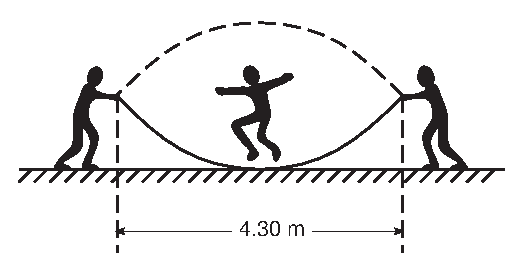
\includegraphics[keepaspectratio,scale=0.75]{Jan2009-Q29}
    \end{center}
    What is the wavelength of this standing wave?
    \begin{multicols}{2}
    \begin{choices}
        \wrongchoice{\SI{2.15}{\meter}}
        \wrongchoice{\SI{4.30}{\meter}}
        \wrongchoice{\SI{6.45}{\meter}}
      \correctchoice{\SI{8.60}{\meter}}
    \end{choices}
    \end{multicols}
\end{question}
}


%% Section June2008
%%--------------------
\element{nysed}{
\begin{question}{June2008-Q25}
    The time required for a wave to complete one full cycle is called the wave's:
    \begin{multicols}{2}
    \begin{choices}
        \wrongchoice{frequency}
        \wrongchoice{velocity}
      \correctchoice{period}
        \wrongchoice{wavelength}
    \end{choices}
    \end{multicols}
\end{question}
}

\element{nysed}{
\begin{question}{June2008-Q27}
    The diagram below represents a transverse wave.
    \begin{center}
    \begin{tikzpicture}[x=0.0625\textwidth]
        %% Graph
        \draw[domain=0:3*pi,smooth,line width=1pt] plot (\x, {sin(\x r)});
        \draw[dashed] (-1.57,0) -- (10.99,0);
        %% Labels
        \node[anchor=north]     at (0,0) {$A$};
        \node[anchor=south]     at (1.57,1) {$B$};
        \node[anchor=north east]at (3.14,0) {$C$};
        \node[anchor=south]     at (4.71,-1) {$D$};
        \node[anchor=north west]at (6.28,0) {$E$};
        \node[anchor=south]     at (7.85,1) {$F$};
        \node[anchor=north]     at (9.42,0) {$G$};
        %% Circles
        \draw[fill] (0,0) circle [radius=1.5pt];
        \draw[fill] (1.57,1) circle [radius=1.5pt];
        \draw[fill] (3.14,0) circle [radius=1.5pt];
        \draw[fill] (4.71,-1) circle [radius=1.5pt];
        \draw[fill] (6.28,0) circle [radius=1.5pt];
        \draw[fill] (7.85,1) circle [radius=1.5pt];
        \draw[fill] (9.42,0) circle [radius=1.5pt];
    \end{tikzpicture}
    \end{center}
    The wavelength of the wave is equal to the distance between points?
    \begin{multicols}{2}
    \begin{choices}
        \wrongchoice{$A$ and $G$}
      \correctchoice{$B$ and $F$}
        \wrongchoice{$C$ and $E$}
        \wrongchoice{$D$ and $F$}
    \end{choices}
    \end{multicols}
\end{question}
}

\element{nysed}{
\begin{question}{June2008-Q30}
    Wave $X$ travels eastward with frequency $f$ and amplitude $A$.
    Wave $Y$, traveling in the same medium,
        interacts with wave $X$ and produces a standing wave.
    Which statement about wave $Y$ is correct?
    \begin{choices}
      \correctchoice{Wave $Y$ must have a frequency of $f$, an amplitude of $A$, and be traveling eastward.}
        \wrongchoice{Wave $Y$ must have a frequency of $2f$, an amplitude of $3A$, and be traveling eastward.}
        \wrongchoice{Wave $Y$ must have a frequency of $3f$, an amplitude of $2A$, and be traveling westward.}
        \wrongchoice{Wave $Y$ must have a frequency of $f$, an amplitude of $A$, and be traveling westward.}
    \end{choices}
\end{question}
}

\element{nysed}{
\begin{question}{June2008-Q31}
    The diagram below represents two pulses approaching each other from opposite directions in the same medium.
    \begin{center}
    \begin{tikzpicture}[yscale=0.6,xscale=0.9]
        \draw[thick] (-4,0) -- (-3,0) parabola bend (-2,1) (-1,0) -- (1,0) parabola bend (2,2) (3,0) -- (4,0);
        \draw[thick,->] (-3,-0.5) -- (-1,-0.5);
        \draw[thick,->] (3,-0.5) -- (1,-0.5);
    \end{tikzpicture}
    \end{center}
    Which diagram best represents the medium after the pulses have passed through each other?
    \begin{choices}
        \AMCboxDimensions{down=-1.25cm}
        \correctchoice{
            \begin{tikzpicture}[yscale=0.6,xscale=0.9]
                \draw[dashed,white!90!black] (-4,-2) rectangle (4,2);
                \draw[thick] (-4,0) -- (-3,0) parabola bend (-2,2) (-1,0)
                                    -- (1,0) parabola bend (2,1) (3,0) -- (4,0);
                \draw[thick,<-] (-3,-0.5) -- (-1,-0.5);
                \draw[thick,<-] (3,-0.5) -- (1,-0.5);
            \end{tikzpicture}
        }
        \wrongchoice{
            \begin{tikzpicture}[yscale=0.6,xscale=0.9]
                \draw[dashed,white!90!black] (-4,-2) rectangle (4,2);
                \draw[thick] (-4,0) -- (-3,0) parabola bend (-2,1) (-1,0)
                                    -- (1,0) parabola bend (2,2) (3,0) -- (4,0);
                \draw[thick,<-] (-3,-0.5) -- (-1,-0.5);
                \draw[thick,<-] (3,-0.5) -- (1,-0.5);
            \end{tikzpicture}
        }
        \wrongchoice{
            \begin{tikzpicture}[yscale=0.6,xscale=0.9]
                \draw[dashed,white!90!black] (-4,-2) rectangle (4,2);
                \draw[thick] (-4,0) -- (-3,0) parabola bend (-2,-1) (-1,0)
                                    -- (1,0) parabola bend (2,-2) (3,0) -- (4,0);
                \draw[thick,<-] (-3,0.5) -- (-1,0.5);
                \draw[thick,<-] (3,0.5) -- (1,0.5);
            \end{tikzpicture}
        }
        \wrongchoice{
            \begin{tikzpicture}[yscale=0.6,xscale=0.9]
                \draw[dashed,white!90!black] (-4,-2) rectangle (4,2);
                \draw[thick] (-4,0) -- (-3,0) parabola bend (-2,-2) (-1,0)
                                    -- (1,0) parabola bend (2,-1) (3,0) -- (4,0);
                \draw[thick,<-] (-3,0.5) -- (-1,0.5);
                \draw[thick,<-] (3,0.5) -- (1,0.5);
            \end{tikzpicture}
        }
    \end{choices}
\end{question}
}

\element{nysed}{
\begin{question}{June2008-Q48}
    The diagram represents a transverse wave traveling to the right through a medium.
    Point $A$ represents a particle of the medium.
    \begin{center}
    \begin{tikzpicture}[x=0.06\textwidth]
        %% Graph
        \draw[domain=0:3*pi,smooth,very thick] plot (\x, {sin(\x r)});
        \draw[dashed] (0,0) -- (9.42,0);
        %% Vectors
        \draw[thick,->] (3.14,1.0) -- (6.28,1.0)
            node[pos=0.5,anchor=south] {$v$};
        %% Labels
        \draw[fill] (5.50,-0.707) circle [radius=1.5pt]
            node[anchor=north west] {$A$};
    \end{tikzpicture}
    \end{center}
    In which direction will particle $A$ move in the next instance of time?
    \begin{multicols}{2}
    \begin{choices}
        \wrongchoice{up}
      \correctchoice{down}
        \wrongchoice{left}
        \wrongchoice{right}
    \end{choices}
    \end{multicols}
\end{question}
}


%% Section Jan2008
%%--------------------
\element{nysed}{
\begin{question}{Jan2008-Q24}
    The product of a wave's frequency and its period is:
    \begin{multicols}{2}
    \begin{choices}
      \correctchoice{one}
        \wrongchoice{its velocity}
        \wrongchoice{its wavelength}
        \wrongchoice{Planck's constant}
    \end{choices}
    \end{multicols}
\end{question}
}

\element{nysed}{
\begin{question}{Jan2008-Q25}
    A periodic wave having a frequency of \SI{5.0}{\hertz} and a speed of \SI{10}{\meter\per\second} has a wavelength of:
    \begin{multicols}{2}
    \begin{choices}
        \wrongchoice{\SI{0.50}{\meter}}
      \correctchoice{\SI{2.0}{\meter}}
        \wrongchoice{\SI{5.0}{\meter}}
        \wrongchoice{\SI{50}{\meter}}
    \end{choices}
    \end{multicols}
\end{question}
}

\element{nysed}{
\begin{question}{Jan2008-Q31}
    Two pulses traveling in the same uniform medium approach each other,
        as shown in the diagram below.
    \begin{center}
    \begin{tikzpicture}[scale=0.8]
        \draw[thick] (0,0) -- (1,0) -- (2,1) -- (3,0) -- (5,0) -- (6,1) -- (7,0) -- (8,0);
        \draw[thick,->] (1,1.2) -- (3,1.2);
        \draw[thick,->] (7,1.2) -- (5,1.2);
    \end{tikzpicture}
    \end{center}
    Which diagram best represents the superposition of the two pulses?
    \begin{multicols}{2}
    \begin{choices}
        \correctchoice{
            \begin{tikzpicture}[scale=0.8]
                \draw[white] (0,0) rectangle (4,2);
                \draw[thick] (0,0) -- (1,0) -- (2,2) -- (3,0) -- (4,0);
            \end{tikzpicture}
        }
        \wrongchoice{
            \begin{tikzpicture}[scale=0.8]
                \draw[white] (0,0) rectangle (4,2);
                \draw[thick] (0,0) -- (1,0) -- (1,1) -- (3,1) -- (3,0) -- (4,0);
            \end{tikzpicture}
        }
        \wrongchoice{
            \begin{tikzpicture}[scale=0.8]
                \draw[white] (0,0) rectangle (4,2);
                \draw[thick] (0,0) -- (1,0) -- (2,1) -- (3,0) -- (4,0);
            \end{tikzpicture}
        }
        \wrongchoice{
            \begin{tikzpicture}[scale=0.8]
                \draw[white] (0,0) rectangle (4,2);
                \draw[thick] (0,0) -- (4,0);
            \end{tikzpicture}
        }
    \end{choices}
    \end{multicols}
\end{question}
}

\element{nysed}{
\begin{question}{Jan2008-Q34}
    Which diagram best represents the shape and direction of a series of wave fronts after they have passed through a small opening in a barrier?
    \begin{multicols}{2}
    \begin{choices}
        \AMCboxDimensions{down=-0.8cm}
        \wrongchoice{
            \begin{tikzpicture}
                \draw[dashed,white!60!black] (-1.5,-1.2) rectangle (1.5,1.2);
                %% incoming
                \foreach \x in {4,8,12} \draw (-\x mm,-1.2) -- (-\x mm,1.2);
                \foreach \y in {-0.75,0.75} \draw[thick,->] (-1.5,\y) -- (-0.2,\y);
                %% barrier
                \draw[pattern=north east lines] (-0.5ex,-1.2) rectangle (0.5ex,-0.2);
                \draw[pattern=north east lines] (-0.5ex,+1.2) rectangle (0.5ex,+0.2);
                %% outgoing
                \draw[thick,->] (0.5ex,+0.75) -- (1.4,+0.2);
                \draw[thick,->] (0.5ex,-0.75) -- (1.4,-0.2);
                \draw[thick,->] (0.5ex,0) -- (1.2,0);
            \end{tikzpicture}
        }
        \wrongchoice{
            \begin{tikzpicture}
                \draw[dashed,white!60!black] (-1.5,-1.2) rectangle (1.5,1.2);
                %% incoming
                \foreach \x in {4,8,12} \draw (-\x mm,-1.2) -- (-\x mm,1.2);
                \foreach \y in {-0.75,0.75} \draw[thick,->] (-1.5,\y) -- (-0.2,\y);
                %% barrier
                \draw[pattern=north east lines] (-0.5ex,-1.2) rectangle (0.5ex,-0.2);
                \draw[pattern=north east lines] (-0.5ex,+1.2) rectangle (0.5ex,+0.2);
                %% outgoing
                \foreach \x in {4,8,12} \draw (1.5,0) ++(140:\x mm) arc(140:220:\x mm);
                \draw[thick,<-] (1.5,0) ++(150:1ex) -- ++(150:1.3);
                \draw[thick,<-] (1.5,0) ++(210:1ex) -- ++(210:1.3);
            \end{tikzpicture}
        }
        \wrongchoice{
            \begin{tikzpicture}
                \draw[dashed,white!60!black] (-1.5,-1.2) rectangle (1.5,1.2);
                %% incoming
                \foreach \x in {4,8,12} \draw (-\x mm,-1.2) -- (-\x mm,1.2);
                \foreach \y in {-0.75,0.75} \draw[thick,->] (-1.5,\y) -- (-0.2,\y);
                %% barrier
                \draw[pattern=north east lines] (-0.5ex,-1.2) rectangle (0.5ex,-0.2);
                \draw[pattern=north east lines] (-0.5ex,+1.2) rectangle (0.5ex,+0.2);
                %% outgoing
                \foreach \x in {4,8,12} {
                    \draw (0.5ex,0) ++(5:\x mm) arc(5:70:\x mm);
                    \draw (0.5ex,0) ++(355:\x mm) arc(355:290:\x mm);
                }
                \draw[thick,<-] (0.5ex,0) ++ (37:1ex) -- ++(37:1.3);
                \draw[thick,<-] (0.5ex,0) ++ (323:1ex) -- ++(323:1.3);
            \end{tikzpicture}
        }
        %% ANS is D
        \correctchoice{
            \begin{tikzpicture}
                \draw[dashed,white!60!black] (-1.5,-1.2) rectangle (1.5,1.2);
                %% incoming
                \foreach \x in {4,8,12} \draw (-\x mm,-1.2) -- (-\x mm,1.2);
                \foreach \y in {-0.75,0.75} \draw[thick,->] (-1.5,\y) -- (-0.2,\y);
                %% barrier
                \draw[pattern=north east lines] (-0.5ex,-1.2) rectangle (0.5ex,-0.2);
                \draw[pattern=north east lines] (-0.5ex,+1.2) rectangle (0.5ex,+0.2);
                %% outgoing
                \foreach \x in {4,8,12} \draw (0.5ex,0) ++(0,\x mm) arc(90:-90:\x mm);
                \foreach \y in {30,330} \draw[thick,->] (0.5ex,0) ++(\y:0.5ex) -- ++(\y:1.3);
            \end{tikzpicture}
        }
    \end{choices}
    \end{multicols}
\end{question}
}


%% Section June2007
%%--------------------
\element{nysed}{
\begin{question}{June2007-Q22}
    The diagram below represents a transverse wave.
    \begin{center}
    \begin{tikzpicture}[x=0.1\textwidth]
        %% Graph
        \draw[domain=0:2*pi,smooth,very thick] plot (\x, {-1*sin(\x r)});
        \draw[] (0,-1.25) -- (0,1.25);
        \draw[] (0,0) -- (6.28,0);
        %% Labels
        \node[anchor=east]      at (0,0) {$A$};
        \node[anchor=east]      at (0,1) {$D$};
        \node[anchor=east]      at (0,-1) {$E$};
        \node[anchor=north west]at (3.14,0) {$B$};
        \node[anchor=north]     at (6.28,0) {$C$};
        %% Dashed
        \draw[dashed] (0,1) -- (4.71,1);
        \draw[dashed] (0,-1) -- (1.57,-1);
        %% Circles
        \draw[fill] (0,1)   circle [radius=1.5pt];
        \draw[fill] (0,0)   circle [radius=1.5pt];
        \draw[fill] (0,-1)  circle [radius=1.5pt];
        \draw[fill] (3.14,0)circle [radius=1.5pt];
        \draw[fill] (6.28,0)circle [radius=1.5pt];
    \end{tikzpicture}
    \end{center}
    The distance between which two points identifies the amplitude of the wave?
    \begin{multicols}{2}
    \begin{choices}
      \correctchoice{$A$ and $E$}
        \wrongchoice{$A$ and $E$}
        \wrongchoice{$A$ and $C$}
        \wrongchoice{$D$ and $E$}
    \end{choices}
    \end{multicols}
\end{question}
}

\element{nysed}{
\begin{question}{June2007-Q23}
    The diagram below represents a periodic wave.
    \begin{center}
    \begin{tikzpicture}[x=0.0556\textwidth]
        %% Graph
        \draw[domain=0:5*pi,smooth,very thick] plot (\x, {cos(\x r)});
        \draw[] (0,-1.25) -- (0,1.25);
        \draw[] (0,0) -- (16.0,0);
        %% Labels
        \node[anchor=south west]at (0,1) {$A$};
        \node[anchor=north west]at (4.71,0) {$P$};
        \node[anchor=south west]at (7.85,0) {$B$};
        \node[anchor=north west]at (10.99,0) {$C$};
        \node[anchor=south]     at (15.7,-1) {$D$};
        %% Circles
        \draw[fill] (0,1)       circle [radius=1.5pt];
        \draw[fill] (4.71,0)    circle [radius=1.5pt];
        \draw[fill] (7.85,0)    circle [radius=1.5pt];
        \draw[fill] (10.99,0)   circle [radius=1.5pt];
        \draw[fill] (15.7,-1)    circle [radius=1.5pt];
    \end{tikzpicture}
    \end{center}
    Which point on the wave is in phase with point $P$?
    \begin{multicols}{4}
    \begin{choices}[o]
        \wrongchoice{$A$}
        \wrongchoice{$B$}
      \correctchoice{$C$}
        \wrongchoice{$D$}
    \end{choices}
    \end{multicols}
\end{question}
}

\element{nysed}{
\begin{question}{June2007-Q27}
    Which type of wave requires a material medium through which to travel?
    \begin{multicols}{2}
    \begin{choices}
      \correctchoice{sound}
        \wrongchoice{electromagnetic}
        \wrongchoice{infrared}
        \wrongchoice{radio}
    \end{choices}
    \end{multicols}
\end{question}
}

\element{nysed}{
\begin{question}{June2007-Q30}
    Two waves having the same frequency and amplitude are traveling in the same medium.
    Maximum constructive interference occurs at points where the phase difference between the two superposed waves is:
    \begin{multicols}{4}
    \begin{choices}
      \correctchoice{\ang{0}}
        \wrongchoice{\ang{90}}
        \wrongchoice{\ang{180}}
        \wrongchoice{\ang{270}}
    \end{choices}
    \end{multicols}
\end{question}
}


%% Section Jan2007
%%--------------------
\element{nysed}{
\begin{question}{Jan2007-Q21}
    If the amplitude of a wave traveling in a rope is doubled,
        the speed of the wave in the rope will:
    \begin{choices}
      \correctchoice{remain the same}
        \wrongchoice{decrease}
        \wrongchoice{increase}
    \end{choices}
\end{question}
}

\element{nysed}{
\begin{question}{Jan2007-Q22}
    Two waves having the same amplitude and frequency are traveling in the same medium.
    Maximum destructive interference will occur when the phase difference between the waves is:
    \begin{multicols}{4}
    \begin{choices}
      \correctchoice{\ang{180}}
        \wrongchoice{\ang{0}}
        \wrongchoice{\ang{270}}
        \wrongchoice{\ang{90}}
    \end{choices}
    \end{multicols}
\end{question}
}

\element{nysed}{
\begin{question}{Jan2007-Q24}
    A ringing bell is located in a chamber.
    When the air is removed from the chamber,
        why can the bell be seen vibrating but \emph{not} be heart?
    \begin{choices}
      \correctchoice{Light waves can travel through a vacuum, but sound waves cannot.}
        \wrongchoice{Light waves travel slower than sound waves.}
        \wrongchoice{Sound waves have greater amplitude than light waves.}
        \wrongchoice{Sound waves have higher frequency than light waves.}
    \end{choices}
\end{question}
}

\element{nysed}{
\begin{question}{Jan2007-Q25}
    As a transverse wave travels through a medium,
        the individual particles of the medium move:
    \begin{choices}
      \correctchoice{perpendicular to the direction of wave travel}
        \wrongchoice{parallel to the direction of wave travel}
        \wrongchoice{in circles}
        \wrongchoice{in ellipses}
    \end{choices}
\end{question}
}

\element{nysed}{
\begin{question}{Jan2007-Q28}
    Parallel wave fronts incident on an opening in a barrier are diffracted.
    For which combination of wavelength and size of opening will diffraction effects be greatest?
    \begin{choices}
      \correctchoice{long wavelength and narrow opening}
        \wrongchoice{long wavelength and wide opening}
        \wrongchoice{short wavelength and narrow opening}
        \wrongchoice{short wavelength and wide opening}
    \end{choices}
\end{question}
}

\element{nysed}{
\begin{question}{Jan2007-Q49}
    The diagram below represents a wave.
    \begin{center}
    \begin{tikzpicture}[x=0.035\textwidth]
        %% Wave
        \draw[domain=0:6*pi,smooth,very thick] plot (\x, {sin(\x r)});
        %% Y Label
        \draw (0,-1.5) -- (0,1.2);
        \draw (18.84,-1.5) -- (18.84,1.2);
        \node[anchor=east] (X1) at (-0.5,1.0) {\SI{0.20}{\meter}};
        \node[anchor=east] (X2) at (-0.5,-1.0) {\SI{-0.20}{\meter}};
        \draw[dashed] (X1) -- (18.84,1.0);
        \draw[dashed] (X2) -- (18.84,-1.0);
        \draw[dashed] (0,0) -- (18.84,0.0);
        %% X Label
        \node[anchor=center] (X4) at (9.42,-1.3) {\SI{6.00}{\meter}};
        \draw[->] (X4) -- (0,-1.3);
        \draw[->] (X4) -- (18.84,-1.3);
    \end{tikzpicture}
    \end{center}
    What is the speed of the wave if its frequency is \SI{8.0}{\hertz}?
    \begin{multicols}{2}
    \begin{choices}
      \correctchoice{\SI{16}{\meter\per\second}}
        \wrongchoice{\SI{48}{\meter\per\second}}
        \wrongchoice{\SI{1.6}{\meter\per\second}}
        \wrongchoice{\SI{3.2}{\meter\per\second}}
    \end{choices}
    \end{multicols}
\end{question}
}


%% Section June2006
%%--------------------
\element{nysed}{
\begin{question}{June2006-Q28}
    The diagram below represents straight fronts passing from deep water into shallow water,
        with a change in speed and direction.
    \begin{center}
    \begin{tikzpicture}
        %% deep water
        \draw[thick,latex-]  (1,2) -- (1,3.5) node[anchor=north] {Deep water};
        \foreach \y in {1.5,2.0,2.5,3.0} \draw[thick] (0,\y) -- ({1.5*(\y+0.66)},\y) -- ++(20:{2.3-1.85*(\y-3)});
        %% boundary
        \draw[line width=2pt] (1,0) -- (7,4) node[pos=0.2,anchor=north,rotate=34] {Boundary};
        \draw[thick,-latex] (1,0) ++(33.69:5.5) ++(290:1ex) -- ++(290:1) node[anchor=north] {Shallow water};
    \end{tikzpicture}
    \end{center}
    Which phenomenon is illustrated in the diagram?
    \begin{multicols}{2}
    \begin{choices}
      \correctchoice{refraction}
        \wrongchoice{reflection}
        \wrongchoice{diffraction}
        \wrongchoice{interference}
    \end{choices}
    \end{multicols}
\end{question}
}

\element{nysed}{
\begin{question}{June2006-Q32}
    Two waves traveling in the same medium and having the same wavelength ($\lambda$) interfere to create a standing wave.
    What is the distance between two consecutive nodes on this standing wave?
    \begin{multicols}{4}
    \begin{choices}
      \correctchoice{$\dfrac{\lambda}{2}$}
        \wrongchoice{$\lambda$}
        \wrongchoice{$\dfrac{\lambda}{4}$}
        \wrongchoice{$\dfrac{3\lambda}{4}$}
    \end{choices}
    \end{multicols}
\end{question}
}

\element{nysed}{
\begin{question}{June2006-Q33}
    An earthquake wave is traveling from west to east through rock.
    If the particles of the rock are vibrating in a north-south direction,
        the wave must be classified as:
    \begin{multicols}{2}
    \begin{choices}
      \correctchoice{transverse}
        \wrongchoice{longitudinal}
        \wrongchoice{a microwave}
        \wrongchoice{a radio wave}
    \end{choices}
    \end{multicols}
\end{question}
}

\element{nysed}{
\begin{question}{June2006-Q46}
    The diagram represents two pulses approaching each other.
    \begin{center}
    \begin{tikzpicture}[scale=0.8]
        \draw[thick] (0,0) -- (1,0) -- (1,1) -- (2,1) -- (2,0) -- (4,0) -- (4,-2) -- (5,-2) -- (5,0) -- (6,0);
        \draw[thick,->] (1,1.5) -- (2,1.5);
        \draw[thick,->] (5,1.5) -- (4,1.5);
    \end{tikzpicture}
    \end{center}
    Which diagram best represents the resultant pulse at the instant the pulses are passing through each other?
    \begin{multicols}{2}
    \begin{choices}
        \AMCboxDimensions{down=-1.5cm}
        \correctchoice{
            \begin{tikzpicture}[scale=0.8]
                \draw[white] (0,-2) rectangle (3,1);
                \draw[thick] (0,0) -- (1,0) -- (1,-1) -- (2,-1) -- (2,0) -- (3,0);
            \end{tikzpicture}
        }
        \wrongchoice{
            \begin{tikzpicture}[scale=0.8]
                \draw[white] (0,-2) rectangle (3,1);
                \draw[thick] (0,0) -- (1,0) -- (1,-2) -- (2,-2) -- (2,0) -- (3,0);
            \end{tikzpicture}
        }
        \wrongchoice{
            \begin{tikzpicture}[scale=0.8]
                \draw[white] (0,-2) rectangle (3,1);
                \draw[thick] (0,0) -- (1,0) -- (1,1) -- (2,1) -- (2,0) -- (3,0);
            \end{tikzpicture}
        }
        \wrongchoice{
            \begin{tikzpicture}[scale=0.8]
                \draw[white] (0,-2) rectangle (3,1);
                \draw[thick] (0,0) -- (3,0);
            \end{tikzpicture}
        }
    \end{choices}
    \end{multicols}
\end{question}
}


%% Section Jan2006
%%--------------------
\element{nysed}{
\begin{question}{Jan2006-Q28}
    A sonar wave is reflected from the ocean floor.
    For which angles of incidence do the wave's angle of reflection equal its angle of incidence?
    \begin{choices}
        \wrongchoice{angles less than \ang{45}, only}
        \wrongchoice{an angle of \ang{45}, only}
        \wrongchoice{angles greater than \ang{45}, only}
      \correctchoice{all angles of incidence}
    \end{choices}
\end{question}
}

\element{nysed}{
\begin{question}{Jan2006-Q29}
    How are electromagnetic waves that are produced by oscillating charges and sound waves that are produced by oscillating tuning forks similar?
    \begin{choices}
      \correctchoice{Both have the same frequency as their respective sources.}
        \wrongchoice{Both require a matter medium for propagation.}
        \wrongchoice{Both are longitudinal waves.}
        \wrongchoice{Both are transverse waves.}
    \end{choices}
\end{question}
}

\element{nysed}{
\begin{question}{Jan2006-Q30}
    The diagram below represents a transverse wave traveling in a string.
    \begin{center}
    \begin{tikzpicture}[x=0.0625\textwidth]
        %% Graph
        \draw[domain=0:4*pi,smooth,line width=1pt] plot (\x, {sin(\x r)});
        \draw (0,0) -- (13.00,0);
        \draw (0,-1.2) -- (0,1.2);
        %% Labels
        \node[anchor=north west]at (0,0)    {$A$};
            \draw[fill] (0,0) circle [radius=1.5pt];
        \node[anchor=north]     at (1.57,1) {$B$};
            \draw[fill] (1.57,1) circle [radius=1.5pt];
        \node[anchor=south west]at (3.14,0) {$C$};
            \draw[fill] (3.14,0) circle [radius=1.5pt];
        \node[anchor=south]     at (4.71,-1) {$D$};
            \draw[fill] (4.71,-1) circle [radius=1.5pt];
        \node[anchor=north west]at (6.28,0){$E$};
            \draw[fill] (6.28,0) circle [radius=1.5pt];
        \node[anchor=north]     at (7.85,1){$F$};
            \draw[fill] (7.85,1) circle [radius=1.5pt];
        \node[anchor=south west]at (9.42,0){$G$};
            \draw[fill] (9.42,0) circle [radius=1.5pt];
        \node[anchor=south]     at (10.99,-1){$H$};
            \draw[fill] (10.99,-1) circle [radius=1.5pt];
    \end{tikzpicture}
    \end{center}
    Which two labeled points are \ang{180} out of phase?
    \begin{multicols}{2}
    \begin{choices}
      \correctchoice{$D$ and $F$}
        \wrongchoice{$B$ and $F$}
        \wrongchoice{$A$ and $D$}
        \wrongchoice{$D$ and $H$}
    \end{choices}
    \end{multicols}
\end{question}
}

\element{nysed}{
\begin{question}{Jan2006-Q32}
    The diagram below represents shallow water waves of constant wavelength passing through two small opening, $A$ and $B$, in a barrier.
    \begin{center}
    %% NOTE: June1996-Q42
    \begin{tikzpicture}
        %% incoming
        \foreach \x in {5,15}
            \draw[dashed] (-4,-\x mm) -- (4,-\x mm);
        \foreach \x in {10,20}
            \draw[thick] (-4,-\x mm) -- (4,-\x mm);
        %% outcoming A
        \foreach \x in {5,15,25}  {
            \draw[dashed] (-1,0.25ex) ++(\x mm,0) arc (0:180:\x mm);
            \draw[dashed] (+1,0.25ex) ++(\x mm,0) arc (0:180:\x mm);
        }
        \foreach \x in {10,20,30} {
            \draw[thick] (-1,0.25ex) ++(\x mm,0) arc (0:180:\x mm);
            \draw[thick] (+1,0.25ex) ++(\x mm,0) arc (0:180:\x mm);
        }
        %% barrier
        \draw[fill=white!50!black] (-4,-0.25ex) rectangle (-1.1,0.25ex);
        \draw[fill=white!50!black] (-0.9,-0.25ex) rectangle (0.9,0.25ex);
        \draw[fill=white!50!black] (1.1,-0.25ex) rectangle (4.0,0.25ex);
        %% labels
        \node[anchor=north] at (-1,0) {$A$};
        \node[anchor=north] at (+1,0) {$B$};
        \fill (6.8mm,25.3mm) circle (2pt) node[anchor=south west] {$P$};
        %% Legend
        \draw (-2.5,-2.5) -- (-1.5,-2.5) node[anchor=west] {Crests};
        \draw[dashed] (0.5,-2.5) -- (1.5,-2.5) node[anchor=west] {Troughs};
    \end{tikzpicture}
    \end{center}
    Which statement best describes the interference at point $P$?
    \begin{choices}
      \correctchoice{It is destructive, and causes a decrease in amplitude.}
        \wrongchoice{It is destructive, and causes a shorter wavelength.}
        \wrongchoice{It is constructive, and causes an increase in amplitude.}
        \wrongchoice{It is constructive, and causes a longer wavelength.}
    \end{choices}
\end{question}
}


%% Section June2005
%%--------------------
\element{nysed}{
\begin{question}{June2005-Q24}
    A transverse wave passes through a uniform material medium from left to right,
        as shown in the diagram below.
    \begin{center}
    \begin{tikzpicture}[x=0.0625\textwidth]
        %% Wave
        \draw[domain=0:3.5*pi,smooth,line width=1pt] plot (\x, {sin(\x r)});
        %% Vector
        \draw[->] (4.0,1.5) -- (7.0,1.5)
            node[pos=0.5,anchor=south] {$v$};
    \end{tikzpicture}
    \end{center}
    Which diagram best represents the direction of vibration of the particles of the medium?
    \begin{multicols}{2}
    \begin{choices}
        \AMCboxDimensions{down=-0.8cm}
        \correctchoice{
            \begin{tikzpicture}
                \draw[dashed,white!90!black] (-1,-1) rectangle (1,1);
                \draw[fill] (0,0) circle (1pt);
                \draw[thick,<->] (270:1) -- (90:1);
            \end{tikzpicture}
        }
        \wrongchoice{
            \begin{tikzpicture}
                \draw[dashed,white!90!black] (-1,-1) rectangle (1,1);
                \draw[fill] (0,0) circle (1pt);
                \draw[thick,<->] (135:1) -- (315:1);
            \end{tikzpicture}
        }
        \wrongchoice{
            \begin{tikzpicture}
                \draw[dashed,white!90!black] (-1,-1) rectangle (1,1);
                \draw[fill] (0,0) circle (1pt);
                \draw[thick,<->] (180:1) -- (0:1);
            \end{tikzpicture}
        }
        \wrongchoice{
            \begin{tikzpicture}
                \draw[dashed,white!90!black] (-1,-1) rectangle (1,1);
                \draw[fill] (0,0) circle (1pt);
                \draw[thick,<->] (225:1) -- (45:1);
            \end{tikzpicture}
        }
    \end{choices}
    \end{multicols}
\end{question}
}

\element{nysed}{
\begin{question}{June2005-Q29}
    If the speed of a wave doubles as it passes from shallow water into deeper water,
        its wavelength will be:
    \begin{multicols}{2}
    \begin{choices}
      \correctchoice{doubled}
        \wrongchoice{unchanged}
        \wrongchoice{halved}
        \wrongchoice{quadrupled}
    \end{choices}
    \end{multicols}
\end{question}
}


%% Section Jan2005
%%--------------------
\element{nysed}{
\begin{question}{Jan2005-Q10}
    The diagram below shows two pulses of equal amplitude, $A$,
        approaching point $P$ along a uniform string.
    \begin{center}
    \begin{tikzpicture}[font=\small,scale=0.90]
        \draw[thick] (-4,0) -- (-3,0) parabola bend (-2,1) (-1,0)
                            -- (1,0) parabola bend (2,-1) (3,0) -- (4,0);
        \draw[dashed] (-4,0) -- (4,0);
        %% Arrows
        \draw[thick,->] (-2,1.3) -- ++(0:1cm);
        \draw[thick,->] (2,-1.3) -- ++(180:1cm);
        %% String label
        \node[anchor=north west] at (-4,0) {String};
        \draw[fill] (0,0) circle (1pt)
            node[anchor=south] {$P$};
        %% Size Labels
        \draw[thick,<->] (-2.0,0) -- (-2.0,1)
            node[pos=0.5,anchor=east] {$A$};
        \draw[thick,<->] (2.0,0) -- (2.0,-1)
            node[pos=0.5,anchor=west] {$A$};
    \end{tikzpicture}
    \end{center}
    When the two pulses meet at $P$,
        the vertical displacement of the string at $P$ will be:
    \begin{multicols}{4}
    \begin{choices}
      \correctchoice{$0$}
        \wrongchoice{$2A$}
        \wrongchoice{$\dfrac{A}{2}$}
        \wrongchoice{$A$}
    \end{choices}
    \end{multicols}
\end{question}
}

\element{nysed}{
\begin{question}{Jan2005-Q11}
    The energy of a water wave is most closely related to its:
    \begin{multicols}{2}
    \begin{choices}
      \correctchoice{amplitude}
        \wrongchoice{frequency}
        \wrongchoice{wavelength}
        \wrongchoice{period}
    \end{choices}
    \end{multicols}
\end{question}
}

\element{nysed}{
\begin{question}{Jan2005-Q12}
    Which form(s) of energy can be transmitted through a vacuum?
    \begin{choices}
      \correctchoice{light, only}
        \wrongchoice{sound, only}
        \wrongchoice{both light and sound}
        \wrongchoice{neither light nor sound}
    \end{choices}
\end{question}
}

\element{nysed}{
\begin{question}{Jan2005-Q18}
    The diagram below represents a wave moving toward the right side of the page.
    \begin{center}
    %% NOTE: Cannot use relative x and y
    \begin{tikzpicture}[xscale=0.25,yscale=0.75]
        \draw[domain=0:3*pi,smooth,line width=1pt] plot (\x, {sin(\x r)});
        \draw[thick,->] (3.14,1.5) -- (6.28,1.5);
    \end{tikzpicture}
    \end{center}
    Which wave shown below could produce a standing wave with the original wave?
    \begin{multicols}{2}
    \begin{choices}
        \AMCboxDimensions{down=-1.0cm}
        \correctchoice{
            \begin{tikzpicture}[xscale=0.25,yscale=0.75]
                \draw[white] (-1.5,-1.5) rectangle (9.42,1.50);
                \draw[domain=0:3*pi,smooth,line width=1pt] plot (\x, {sin(\x r)});
                \draw[->] (6.28,1.5) -- (3.14,1.5);
            \end{tikzpicture}
        }
        \wrongchoice{
            \begin{tikzpicture}[xscale=0.25,yscale=0.75]
                \draw[white] (-1.5,-1.5) rectangle (9.42,1.50);
                \draw[domain=0:3*pi,smooth,line width=1pt] plot (\x, {sin(\x r)});
                \draw[thick,->] (3.14,1.5) -- (6.28,1.5);
            \end{tikzpicture}
        }
        \wrongchoice{
            \begin{tikzpicture}[xscale=0.25,yscale=0.75]
                \draw[white] (-1.5,-1.5) rectangle (9.42,1.50);
                \draw[domain=0:3*pi,smooth,line width=1pt] plot (\x, {1.5*sin(\x r)});
                \draw[thick,->] (3.14,1.5) -- (6.28,1.5);
            \end{tikzpicture}
        }
        \wrongchoice{
            \begin{tikzpicture}[xscale=0.25,yscale=0.75]
                \draw[white] (-1.5,-1.5) rectangle (9.42,1.50);
                \draw[domain=0:3*pi,smooth,line width=1pt] plot (\x, {1.5*sin(\x r)});
                \draw[thick,->] (6.28,1.5) -- (3.14,1.5);
            \end{tikzpicture}
        }
    \end{choices}
    \end{multicols}
\end{question}
}

\element{nysed}{
\begin{question}{Jan2005-Q48}
    Which diagram below does \emph{not} represent a periodic wave?
    \begin{multicols}{2}
    \begin{choices}
        \AMCboxDimensions{down=-1.0cm}
        \wrongchoice{
            \begin{tikzpicture}[xscale=0.25]
                \draw[very thick] (0,0) -- (1,1) -- (2,1) -- (3,0) -- (4,-1) -- (5,-1) -- (6,0);
                \draw[very thick] (6,0) -- (7,1) -- (8,1) -- (9,0) -- (10,-1) -- (11,-1) -- (12,0);
                \draw[dashed] (0,-1) -- (0,1);
                \draw[dashed] (0,0) -- (12,0);
            \end{tikzpicture}
        }
        \wrongchoice{
            \begin{tikzpicture}[xscale=0.25]
                \draw[very thick] (0,0) -- (1,1) -- (2,0) -- (3,-1) -- (4,0) -- (5,1) -- (6,0);
                \draw[very thick] (6,0) -- (7,-1) -- (8,0) -- (9,1) -- (10,0) -- (11,-1) -- (12,0);
                \draw[dashed] (0,-1) -- (0,1);
                \draw[dashed] (0,0) -- (12,0);
            \end{tikzpicture}
        }
        \wrongchoice{
            \begin{tikzpicture}[xscale=0.15]
                \draw[domain=0:6*pi,smooth,very thick] plot (\x, {sin(\x r)});
                \draw[dashed] (0,-1) -- (0,1);
                \draw[dashed] (0,0) -- (18.84,0);
            \end{tikzpicture}
        }
        \correctchoice{
            \begin{tikzpicture}[xscale=0.15]
                %% this required much testing
                \draw[domain=0:6*pi,samples=100,very thick] plot (\x, {sin(0.03*\x*\x r)});
                %\draw[domain=0:6*pi,samples=100,very thick] plot (\x, {sin(2.2*sqrt(\x) r)});
                \draw[dashed] (0,-1) -- (0,1);
                \draw[dashed] (0,0) -- (18.84,0);
            \end{tikzpicture}
        }
    \end{choices}
    \end{multicols}
\end{question}
}


%% Section June2004
%%--------------------
\element{nysed}{
\begin{question}{June2004-Q26}
    A single vibratory disturbance moving through a medium is called:
    \begin{multicols}{2}
    \begin{choices}
      \correctchoice{a pulse}
        \wrongchoice{a node}
        \wrongchoice{an antinode}
        \wrongchoice{a standing wave}
    \end{choices}
    \end{multicols}
\end{question}
}

\element{nysed}{
\begin{question}{June2004-Q32}
    A source of waves and an observer are moving relative to each other.
    The observer will detect a steadily increasing frequency if:
    \begin{choices}
      \correctchoice{he accelerates toward the source}
        \wrongchoice{he moves toward the source at a constant speed}
        \wrongchoice{the source accelerates away from him}
        \wrongchoice{the source moves away from him at a constant speed}
    \end{choices}
\end{question}
}

\element{nysed}{
\begin{question}{June2004-Q33}
    Which wave diagram has \emph{both} wavelength ($\lambda$) and amplitude ($A$) labeled correctly?
    \begin{multicols}{2}
    \begin{choices}
        \AMCboxDimensions{down=-1.00cm}
        \correctchoice{
            \begin{tikzpicture}[x=0.05\columnwidth,font=\footnotesize]
                \draw[domain=0:4*pi,smooth,line width=1pt] plot (\x, {sin(\x r)});
                \draw[dashed] (-1.57,0) -- (13.3,0);
                %% Amplitude
                \draw[dashed] (-1.57,1) -- (1.57,1);
                \draw[<->] (-1.57,0) -- (-1.57,1)
                    node[pos=0.5,anchor=center,fill=white] {$A$};
                %% Wavelength
                \draw[dashed] (6.28,0) -- (6.28,1.5);
                \draw[dashed] (12.56,0) -- (12.56,1.5);
                \draw[<->] (6.28,1.5) -- (12.56,1.5)
                    node[pos=0.5,anchor=center,fill=white] {$\lambda$};
            \end{tikzpicture}
        }
        \wrongchoice{
            \begin{tikzpicture}[x=0.05\columnwidth,font=\footnotesize]
                \draw[domain=0:4*pi,smooth,line width=1pt] plot (\x, {sin(\x r)});
                \draw[dashed] (-1.57,0) -- (13.3,0);
                %% Amplitude
                \draw[dashed] (-1.57,1) -- (1.57,1);
                \draw[<->] (-1.57,0) -- (-1.57,1)
                    node[pos=0.5,anchor=center,fill=white] {$A$};
                %% Wavelength
                \draw[dashed] (6.28,0) -- (6.28,1.5);
                \draw[dashed] (9.42,0) -- (9.42,1.5);
                \draw[<->] (6.28,1.5) -- (9.42,1.5)
                    node[pos=0.5,anchor=center,fill=white] {$\lambda$};
            \end{tikzpicture}
        }
        \wrongchoice{
            \begin{tikzpicture}[x=0.05\columnwidth,font=\footnotesize]
                \draw[domain=0:4*pi,smooth,line width=1pt] plot (\x, {sin(\x r)});
                \draw[dashed] (-0.79,0) -- (13.3,0);
                %% Amplitude
                \draw[dashed] (-1.57,1) -- (1.57,1);
                \draw[dashed] (-1.57,-1) -- (4.71,-1);
                \draw[<->] (-1.57,-1) -- (-1.57,1)
                    node[pos=0.5,anchor=center,fill=white] {$A$};
                %% Wavelength
                \draw[dashed] (6.28,0) -- (6.28,1.5);
                \draw[dashed] (12.56,0) -- (12.56,1.5);
                \draw[<->] (6.28,1.5) -- (12.56,1.5)
                    node[pos=0.5,anchor=center,fill=white] {$\lambda$};
            \end{tikzpicture}
        }
        \wrongchoice{
            \begin{tikzpicture}[x=0.05\columnwidth,font=\footnotesize]
                \draw[domain=0:4*pi,smooth,line width=1pt] plot (\x, {sin(\x r)});
                \draw[dashed] (-1.57,0) -- (13.3,0);
                %% Amplitude
                \draw[dashed] (-1.57,1) -- (1.57,1);
                \draw[dashed] (-1.57,-1) -- (4.71,-1);
                \draw[<->] (-1.57,-1) -- (-1.57,1)
                    node[pos=0.5,anchor=center,fill=white] {$A$};
                %% Wavelength
                \draw[dashed] (6.28,0) -- (6.28,1.5);
                \draw[dashed] (9.42,0) -- (9.42,1.5);
                \draw[<->] (6.28,1.5) -- (9.42,1.5)
                    node[pos=0.5,anchor=center,fill=white] {$\lambda$};
            \end{tikzpicture}
        }
    \end{choices}
    \end{multicols}
\end{question}
}

\element{nysed}{
\begin{question}{June2004-Q35}
    The diagram below represents two waves of equal amplitude and frequency approaching point $P$ as they move through the same medium.
    \begin{center}
    \begin{tikzpicture}[x=0.03\textwidth,yscale=0.75]
        %% Graph
        \draw[domain=-5*pi:-1*pi,smooth,line width=1pt] plot (\x, {sin(\x r)});
        \draw[domain=1*pi:5*pi,smooth,line width=1pt] plot (\x, {sin(\x r)});
        \draw[dashed] (-16.5,0) -- (16.5,0);
        %% Vectors
        \draw[thick,->] (-12.56,1.4) -- (-6.28,1.4);
        \draw[thick,->] (12.56,1.4) -- (6.28,1.4);
        %% Labels
        \draw[fill] (0,0) circle [radius=1.5pt]
            node[anchor=north] {$P$};
    \end{tikzpicture}
    \end{center}
    As the two waves pass through each other,
        the medium at point $P$ will:
    \begin{choices}
        \wrongchoice{vibrate up and down}
        \wrongchoice{vibrate left and right}
        \wrongchoice{vibrate into and out of the page}
      \correctchoice{remain stationary}
    \end{choices}
\end{question}
}


%% Section Jan2004
%%--------------------
\element{nysed}{
\begin{question}{Jan2004-Q22}
    A student strikes the top rope of a volleyball net,
        sending a single vibratory disturbance along the length of the net,
        as shown in the diagram below.
    \begin{center}
    \begin{tikzpicture}
        %% Pole
        \draw[pattern=north east lines] (-0.2cm,2.5) rectangle (-0.5cm,-3);
        %% Net
        \draw[thin,step=0.25] (0,0) grid (4.2,2);
        \draw[thick] (-0.2,2.2) -- (4.2,2.2);
        \draw[thick] (-0.2,-0.2) -- (4.2,-0.2);
        \draw[thick] (-0,-0.2) -- (0,2.2);
        %% Vectors
        \draw[thick,<-] (1.5,2.25) -- ++(90:1) node[anchor=north east,font=\small] {Strike};
        \draw[thick,->] (2,2.5) -- ++(0:2) node[pos=0.5,anchor=south,font=\small] {Disturbance};
    \end{tikzpicture}
    \end{center}
    This instance is best described as:
    \begin{choices}
      \correctchoice{a pulse}
        \wrongchoice{a periodic wave}
        \wrongchoice{a longitudinal wave}
        \wrongchoice{an electromagnetic wave}
    \end{choices}
\end{question}
}

\element{nysed}{
\begin{question}{Jan2004-Q25}
    If the frequency of a periodic wave is doubled,
        the period of the wave will be:
    \begin{multicols}{2}
    \begin{choices}
      \correctchoice{halved}
        \wrongchoice{doubled}
        \wrongchoice{quartered}
        \wrongchoice{quadrupled}
    \end{choices}
    \end{multicols}
\end{question}
}

\element{nysed}{
\begin{question}{Jan2004-Q30}
    Two pulses, $A$ and $B$, travel toward each other along the same rope, as shown below.
    \begin{center}
    \begin{tikzpicture}
        %% grid
        \draw[gray,very thin,step=0.5] (-0.1,-2) grid (6,2);
        %% labels
        \draw[thick] (0,-2) -- (0,2);
        \foreach \y in {-2,-1,0,1,2} \node[anchor=east] at (0,\y) {$\y$};
        \node[anchor=south,rotate=90,font=\large] at (-2em,0) {Units};
        %% waves A
        \draw[line width=1pt,black] plot[domain=0:3,samples=100] (\x,{2*exp(-5*(\x-1.5)^2)});
        \node[anchor=south] at (1.5,0) {$A$};
        \draw[thick,->] (1,2.25) -- (2,2.25) node[pos=0.5,anchor=south] {$v$};
        %% waves B
        \draw[line width=1pt,black] plot[domain=3:6,samples=100] (\x,{-exp(-5*(\x-4.5)^2)});
        \node[anchor=north] at (4.5,0) {$B$};
        \draw[thick,->] (5,-1.25) -- (4,-1.25) node[pos=0.5,anchor=north] {$v$};
        %% point X
        \fill (3,0) circle (2pt) node[anchor=north] {$X$};
    \end{tikzpicture}
    \end{center}
    When the centers of the two pulses meet at point $X$,
        the amplitude at the center of the resultant pulses will be:
    \begin{multicols}{2}
    \begin{choices}
      \correctchoice{\num[retain-explicit-plus]{+1} unit}
        \wrongchoice{\num[retain-explicit-plus]{+2} unit}
        \wrongchoice{\num[retain-explicit-plus]{+0} unit}
        \wrongchoice{\num[retain-explicit-plus]{-1} unit}
    \end{choices}
    \end{multicols}
\end{question}
}

\element{nysed}{
\begin{question}{Jan2004-Q32}
    The superposition of two waves traveling in the same medium produces a standing wave pattern if the two waves have:
    \begin{choices}
      \correctchoice{the same frequency, the same amplitude, and travel in opposite directions.}
        \wrongchoice{the same frequency, the same amplitude, and travel in the same direction.}
        \wrongchoice{the same frequency, different amplitudes, and travel in the same direction.}
        \wrongchoice{the same frequency, different amplitudes, and travel in opposite directions.}
    \end{choices}
\end{question}
}


%% Section June2003
%%--------------------
\element{nysed}{
\begin{question}{June2003-Q23}
    A change in the speed of a wave as it enters a new medium produces a change in:
    \begin{multicols}{2}
    \begin{choices}
      \correctchoice{wavelength}
        \wrongchoice{frequency}
        \wrongchoice{period}
        \wrongchoice{phase}
    \end{choices}
    \end{multicols}
\end{question}
}

\element{nysed}{
\begin{question}{June2003-Q25}
    A tuning fork oscillates with frequency of \SI{256}{\hertz} after being struck by a rubber hammer.
    Which phrase best describes the sound waves produced by this oscillating tuning fork?
    \begin{choices}
      \correctchoice{mechanical waves that require a medium for transmission}
        \wrongchoice{mechanical waves that require no medium for transmission}
        \wrongchoice{electromagnetic waves that require a medium for transmission}
        \wrongchoice{electromagnetic waves that require no medium for transmission}
    \end{choices}
\end{question}
}

\element{nysed}{
\begin{question}{June2003-Q29}
    Standing waves in water are produced most often by periodic water waves:
    \begin{choices}
      \correctchoice{being absorbed at the boundary with a new medium.}
        \wrongchoice{refracting at a boundary with a new medium.}
        \wrongchoice{diffracting around a barrier.}
        \wrongchoice{reflecting from a barrier.}
    \end{choices}
\end{question}
}

\element{nysed}{
\begin{question}{June2003-Q45}
    The diagram below shows two pulses, $A$ and $B$,
        approaching each other in a uniform medium.
    \begin{center}
    \begin{tikzpicture}[scale=0.90]
        %% Axis
        \draw (0,-1) -- (6,-1);
        \draw (0,-1) -- (0,2);
        %% Axis Labels
        \node[anchor=east] at (0,-1) {-1};
        \node[anchor=east] at (0,0) {0};
        \node[anchor=east] at (0,1) {1};
        \node[anchor=east] at (0,2) {2};
        %% A and B waves
        \draw (0,0) -- (1,0) -- (1,1) -- (2,1) -- (2,0) -- (4,0) -- (4,1) -- (5,1) -- (5,0) -- (6,0);
        \node[anchor=center] at (1.5,0.5) {$A$};
        \node[anchor=center] at (4.5,0.5) {$B$};
        %% Vectors
        \draw[ultra thick,->] (2.0,0.5) -- ++ (0:0.5);
        \draw[ultra thick,->] (4.0,0.5) -- ++ (180:0.5);
        %\draw[->] (1.5,1.5) -- ++ (0:1);
        %\draw[->] (4.5,1.5) -- ++ (180:1);
    \end{tikzpicture}
    \end{center}
    Which diagram best represents the superposition of the two pulses?
    %[\emph{Please note:} options are drawn at half scale]
    \begin{multicols}{2}
    \begin{choices}
        \AMCboxDimensions{down=-0.70cm}
        \correctchoice{
            \begin{tikzpicture}[scale=0.4,font=\small]
                %% Axis
                \draw (0,-1) -- (6,-1);
                \draw (0,-1) -- (0,2);
                %% Axis Labels
                \node[anchor=east] at (0,-1) {-1};
                \node[anchor=east] at (0,0) {0};
                \node[anchor=east] at (0,1) {1};
                \node[anchor=east] at (0,2) {2};
                %% Superposition
                \draw (0,0) -- (2.5,0) -- (2.5,2) -- (3.5,2) -- (3.5,0) -- (6,0);
            \end{tikzpicture}
        }
        \wrongchoice{
            \begin{tikzpicture}[scale=0.4,font=\small]
                %% Axis
                \draw (0,-1) -- (6,-1);
                \draw (0,-1) -- (0,2);
                %% Axis Labels
                \node[anchor=east] at (0,-1) {-1};
                \node[anchor=east] at (0,0) {0};
                \node[anchor=east] at (0,1) {1};
                \node[anchor=east] at (0,2) {2};
                %% Superposition: triangle
                \draw (0,0) -- (2,0) -- (3,2) -- (4,0) -- (6,0);
            \end{tikzpicture}
        }
        \wrongchoice{
            \begin{tikzpicture}[scale=0.4,font=\small]
                %% Axis
                \draw (0,-1) -- (6,-1);
                \draw (0,-1) -- (0,2);
                %% Axis Labels
                \node[anchor=east] at (0,-1) {-1};
                \node[anchor=east] at (0,0) {0};
                \node[anchor=east] at (0,1) {1};
                \node[anchor=east] at (0,2) {2};
                %% Superposition: long and flat
                \draw (0,0) -- (1,0) -- (1,0.5) -- (4,0.5) -- (4,0) -- (6,0);
            \end{tikzpicture}
        }
        \wrongchoice{
            \begin{tikzpicture}[scale=0.4,font=\small]
                %% Axis
                \draw (0,-1) -- (6,-1);
                \draw (0,-1) -- (0,2);
                %% Axis Labels
                \node[anchor=east] at (0,-1) {-1};
                \node[anchor=east] at (0,0) {0};
                \node[anchor=east] at (0,1) {1};
                \node[anchor=east] at (0,2) {2};
                %% Superposition: spiky and short
                \draw (0,0) -- (2,0) -- (2,2) -- (2.4,2) -- (2.4,0.5) -- (3.6,0.5) -- (3.6,2) -- (4.0,2) -- (4,0) -- (6,0);
            \end{tikzpicture}
        }
    \end{choices}
    \end{multicols}
\end{question}
}


%% Section Jan2003
%%--------------------
\element{nysed}{
\begin{question}{Jan2003-Q24}
    A periodic wave transfers:
    \begin{choices}
      \correctchoice{energy, only}
        \wrongchoice{mass, only}
        \wrongchoice{both mass and energy}
        \wrongchoice{neither mass nor energy}
    \end{choices}
\end{question}
}

\element{nysed}{
\begin{question}{Jan2003-Q27}
    A motor is used to produce \num{4.0} waves each
        second in a string.
    What is the frequency of the waves?
    \begin{multicols}{2}
    \begin{choices}
      \correctchoice{\SI{4.0}{\hertz}}
        \wrongchoice{\SI{0.25}{\hertz}}
        \wrongchoice{\SI{25}{\hertz}}
        \wrongchoice{\SI{15}{\hertz}}
    \end{choices}
    \end{multicols}
\end{question}
}

\element{nysed}{
\begin{question}{Jan2003-Q28}
    The diagram below shows a periodic wave.
    \begin{center}
    \begin{tikzpicture}[x=0.0625\textwidth]
        %% Graph
        \draw[domain=0:4*pi,smooth,line width=1pt] plot (\x, {sin(\x r)});
        \draw (-0.2,0) -- (13.00,0);
        \draw (0,-1.2) -- (0,1.2);
        %% Labels
        \node[anchor=south west]    at (2.84,0.3)    {$A$};
            \draw[fill] (2.84,0.3) circle [radius=1.5pt];
        \node[anchor=north east]    at (3.44,-0.3)    {$B$};
            \draw[fill] (3.44,-0.3) circle [radius=1.5pt];
        \node[anchor=south east]    at (6.58,0.3)    {$C$};
            \draw[fill] (6.58,0.3) circle [radius=1.5pt];
        \node[anchor=south west]    at (9.12,0.3)    {$D$};
            \draw[fill] (9.12,0.3) circle [radius=1.5pt];
    \end{tikzpicture}
    \end{center}
    Which points are in phase with each other?
    \begin{multicols}{2}
    \begin{choices}
      \correctchoice{$A$ and $D$}
        \wrongchoice{$A$ and $C$}
        \wrongchoice{$B$ and $C$}
        \wrongchoice{$C$ and $D$}
    \end{choices}
    \end{multicols}
\end{question}
}

\element{nysed}{
\begin{question}{Jan2003-Q29}
    A surfacing whale in an aquarium produces water wave crests having an amplitude of \SI{1.2}{\meter} every \SI{0.40}{\second}.
    If the water wave travels at \SI{4.5}{\meter\per\second},
        the wavelength of the wave is:
    \begin{multicols}{2}
    \begin{choices}
      \correctchoice{\SI{1.8}{\meter}}
        \wrongchoice{\SI{2.4}{\meter}}
        \wrongchoice{\SI{3.0}{\meter}}
        \wrongchoice{\SI{11}{\meter}}
    \end{choices}
    \end{multicols}
\end{question}
}

\element{nysed}{
\begin{question}{Jan2003-Q32}
    A radar gun can determine the speed of a moving automobile by measuring the difference in frequency between emitted and reflected radar waves.
    This process illustrates:
    \begin{choices}
      \correctchoice{the Doppler effect}
        \wrongchoice{resonance}
        \wrongchoice{diffraction}
        \wrongchoice{refraction}
    \end{choices}
\end{question}
}

\element{nysed}{
\begin{question}{Jan2003-Q33}
    The diagram below shows a standing wave.
    \begin{center}
    \begin{tikzpicture}[x=0.0625\textwidth]
        %% Graph
        \draw[domain=0:3*pi,smooth,thick] plot (\x, {sin(\x r)});
        \draw[domain=0:3*pi,smooth,thick] plot (\x, {-1*sin(\x r)});
        \draw (0,-1.2) -- (0,1.2);
        \draw (9.42,-1.2) -- (9.42,1.2);
        \node[anchor=east,fill,pattern=north east lines,minimum width=0.1cm, minimum height=2.4cm] at (0,0) {};
        \node[anchor=west,fill,pattern=north east lines,minimum width=0.1cm, minimum height=2.4cm] at (9.42,0) {};
        %% Labels
        \node[pin=270:$A$]  at (3.14,0) {};
            \draw[fill] (3.14,0) circle [radius=1.5pt];
    \end{tikzpicture}
    \end{center}
    Point $A$ on the standing wave is:
    \begin{choices}
      \correctchoice{an antinode resulting from destructive interference}
        \wrongchoice{an antinode resulting from constructive interference}
        \wrongchoice{a node resulting from destructive interference}
        \wrongchoice{a node resulting from constructive interference}
    \end{choices}
\end{question}
}

\element{nysed}{
\begin{question}{Jan2003-Q50}
    The diagram below shows two pulses traveling toward each other in a uniform medium.
    \begin{center}
    \begin{tikzpicture}
        \draw[thick] (-3,0) -- (-2,0) -- (-2,1) -- (-1,1) -- (-1,0) -- (1,0) parabola bend (1.5,-1) (2,0) -- (3,0);
        %% Arrows
        \draw[thick,->] (-1.5,1.2) -- ++ (0:1);
        \draw[thick,->] (1.5,-1.2) -- ++ (180:1);
        %% Size Labels
        \draw[fill] (0,0) circle (2pt)
            node[anchor=north] {$X$};
    \end{tikzpicture}
    \end{center}
    Which diagram best represents the medium when the pulses meet at point $X$?
    \begin{multicols}{2}
    \begin{choices}
        \AMCboxDimensions{down=-1.5em}
        \correctchoice{
            \begin{tikzpicture}
                \draw[white] (-1.5,-1.5em) rectangle (1.5,1cm);
                \draw (-1.5,0) -- (-0.5,0) -- (-0.5,1) parabola bend (0,0) (0.5,1) -- (0.5,0) -- (1.5,0);
                \draw[fill] (0,0) circle (2pt) node[anchor=north] {$X$};
            \end{tikzpicture}
        }
        \wrongchoice{
            \begin{tikzpicture}
                \draw[white] (-1.5,-1.5em) rectangle (1.5,1cm);
                \draw (-1.5,0) -- (-0.5,0) parabola bend (0,1) (0.5,0) -- (1.5,0);
                \draw[fill] (0,1) circle (2pt) node[anchor=north] {$X$};
            \end{tikzpicture}
        }
        \wrongchoice{
            \begin{tikzpicture}
                \draw[white] (-1.5,-1.5em) rectangle (1.5,1cm);
                \draw (-1.5,0) -- (-0.5,0) -- (-0.5,0.25) -- (0.5,0.25) -- (0.5,0) -- (1.5,0);
                \draw[fill] (0,0.25) circle (2pt) node[anchor=north] {$X$};
            \end{tikzpicture}
        }
        \wrongchoice{
            \begin{tikzpicture}
                \draw[white] (-1.5,-1.5em) rectangle (1.5,1cm);
                \draw (-1.5,0) -- (1.5,0);
                \draw[fill] (0,0) circle (2pt) node[anchor=north] {$X$};
            \end{tikzpicture}
        }
    \end{choices}
    \end{multicols}
\end{question}
}


%% Section Aug2002
%%--------------------
\element{nysed}{
\begin{question}{Aug2002-Q15}
    A physics student notices that \num{4.0} waves arrive at the beach every \SI{20}{\second}.
    The frequency of these waves is:
    \begin{multicols}{2}
    \begin{choices}
      \correctchoice{\SI{0.20}{\hertz}}
        \wrongchoice{\SI{5.0}{\hertz}}
        \wrongchoice{\SI{16}{\hertz}}
        \wrongchoice{\SI{80}{\hertz}}
    \end{choices}
    \end{multicols}
\end{question}
}

\element{nysed}{
\begin{question}{Aug2002-Q17}
    The diagram below shows two points,
        $A$ and $B$, on a wave train.
    \begin{center}
    \begin{tikzpicture}[x=0.0625\textwidth]
        %% Graph
        \draw[domain=0:4*pi,smooth,line width=1pt] plot (\x, {sin(\x r)});
        \draw[dashed] (0,0) -- (14.13,0);
        %% Labels
        \draw[fill] (0.00,0) circle (2.5pt)
            node[anchor=south east] {$A$};
        \draw[fill] (9.42,0) circle (2.5pt)
            node[anchor=south west] {$B$};
    \end{tikzpicture}
    \end{center}
    How many wavelengths separate point $A$ and point $B$?
    \begin{multicols}{4}
    \begin{choices}
        \wrongchoice{\num{1.0}}
      \correctchoice{\num{1.5}}
        \wrongchoice{\num{3.0}}
        \wrongchoice{\num{0.75}}
    \end{choices}
    \end{multicols}
\end{question}
}

\element{nysed}{
\begin{question}{Aug2002-Q18}
    In a demonstration,
        a vibrating tuning fork causes a nearby second tuning fork to begin to vibrate with the same frequency.
    Which wave phenomenon is illustrated by this demonstration?
    \begin{choices}
        \wrongchoice{The Doppler effect}
        \wrongchoice{nodes}
      \correctchoice{resonance}
        \wrongchoice{interference}
    \end{choices}
\end{question}
}

\element{nysed}{
\begin{question}{Aug2002-Q19}
    The diagram below shows wave fronts spreading into the region behind a barrier.
    \begin{center}
    \begin{tikzpicture}
        %% Incoming
        \foreach \i in {0,0.66,1.33} {
            \draw[very thick] (\i,0) -- (\i,4);
        }
        \draw[very thick,->] (0,3) -- (1.2,3);
        \draw[very thick,->] (0,1) -- (1.2,1);
        %% Barrier
        \draw[fill=white!45!black] (1.8,0) rectangle (2,1.8);
        \draw[fill=white!45!black] (1.8,2) rectangle (2,4);
        %% Outgoing
        \foreach \i in {0.66,1.33,2.00} {
            \draw[] (2,2)++(90:\i) arc (90:-90:\i);
        }
        \draw[very thick,->] (2,2)++(-45:0.5) --++ (-45:1.4);
        \draw[very thick,->] (2,2)++(+45:0.5) --++ (+45:1.4);
    \end{tikzpicture}
    \end{center}
    Which wave phenomenon is represented in the diagram?
    \begin{multicols}{2}
    \begin{choices}
        \wrongchoice{reflection}
        \wrongchoice{refraction}
      \correctchoice{diffraction}
        \wrongchoice{standing waves}
    \end{choices}
    \end{multicols}
\end{question}
}

\element{nysed}{
\begin{question}{Aug2002-Q20}
    The diagram below represents the wave pattern produced by two sources located at points $A$ and $B$.
    \begin{center}
    \begin{tikzpicture}
        %% Wave Fronts
        \foreach \r in {0.66,1.00,1.33,1.66} {
            \draw (-1,0) circle (\r);
            \draw (+1,0) circle (\r);
        }
        %% Sources
        \draw[fill] (-1,0) circle (1.5pt)
            node[anchor=east] {$A$};
        \draw[fill] (+1,0) circle (1.5pt)
            node[anchor=west] {$B$};
        %% Legend
        \node[anchor=west] at (-0.0,2.0) {Wave fronts};
        \draw (-1.5,2.0) -- (0.0,2.0);
    \end{tikzpicture}
    \end{center}
    Which phenomenon occurs at the intersections of the circular wave fronts?
    \begin{multicols}{2}
    \begin{choices}
        \wrongchoice{diffraction}
      \correctchoice{interference}
        \wrongchoice{refraction}
        \wrongchoice{reflection}
    \end{choices}
    \end{multicols}
\end{question}
}


%% Section June2002
%%--------------------
\element{nysed}{
\begin{question}{June2002-Q26}
    The diagram below represents a periodic wave.
    \begin{center}
    \begin{tikzpicture}[x=0.0707\textwidth]
        %% Graph
        \draw[domain=0:4*pi,smooth,line width=1pt] plot (\x, {sin(\x r)});
        \draw[dashed] (0,0) -- (12.56,0);
        %% Labels
        \draw[fill] (2.36,0.707) circle [radius=2pt]
            node[anchor=south west] {$A$};
        \draw[fill] (4.71,-1.00) circle [radius=2pt]
            node[anchor=north] {$B$};
        \draw[fill] (7.07,0.707) circle [radius=2pt]
            node[anchor=south east] {$C$};
        \draw[fill] (9.42,0.00) circle [radius=2pt]
            node[anchor=south west] {$D$};
        \draw[fill] (11.0,-1.00) circle [radius=2pt]
            node[anchor=north] {$E$};
    \end{tikzpicture}
    \end{center}
    Which two points on the wave are in phase?
    \begin{multicols}{2}
    \begin{choices}
        \wrongchoice{$A$ and $C$}
        \wrongchoice{$B$ and $D$}
        \wrongchoice{$A$ and $C$}
      \correctchoice{$B$ and $E$}
    \end{choices}
    \end{multicols}
\end{question}
}

\element{nysed}{
\begin{question}{June2002-Q28}
    A standing wave pattern is produced when a guitar string is plucked.
    Which characteristic of the standing wave immediately begins to decrease:
    \begin{multicols}{2}
    \begin{choices}
        \wrongchoice{speed}
        \wrongchoice{wavelength}
        \wrongchoice{frequency}
      \correctchoice{amplitude}
    \end{choices}
    \end{multicols}
\end{question}
}

\element{nysed}{
\begin{question}{June2002-Q35}
    Which diagram below best represents the phenomenon of diffraction?
    \begin{multicols}{2}
    \begin{choices}
        \AMCboxDimensions{down=-1.0cm}
        \correctchoice{
            \begin{tikzpicture}[scale=0.75]
                \draw[dashed,white!60!black] (-2.2,-1.5) rectangle (2.2,2.2);
                %% Barrier
                \fill (-2,0) rectangle (-0.1,0.1);
                \fill (+2,0) rectangle (+0.1,0.1);
                %% incoming
                \foreach \x in {5,10,15} \draw (-2,-\x mm) -- (2,-\x mm);
                \foreach \x in {-1,1} \draw[thick,->] (\x,-1.25) -- (\x,-0.25);
                %% diffraction
                \foreach \x in {5,10,15,20} \draw (0,0.1) ++(0:\x mm) arc (0:180:\x mm);
                \foreach \x in {45,135} \draw[thick,->] (0,0.1) ++(\x:1ex) -- ++(\x:1);
            \end{tikzpicture}
        }
        \wrongchoice{
            \begin{tikzpicture}[x=0.447cm]
                \draw[dashed,white!60!black] (-0.5,-1.39) rectangle (6.8,1.39);
                %% line
                \draw (0,0) -- (6.28,0);
                %% sin curve
                \draw[domain=0:2*pi,smooth,thick] plot (\x, {1.1*sin(\x r)});
                \draw[domain=0:2*pi,smooth,dashed] plot (\x, {-1.1*sin(\x r)});
            \end{tikzpicture}
        }
        \wrongchoice{
            \begin{tikzpicture}[scale=0.75]
                \draw[dashed,white!60!black] (-2.2,-1.5) rectangle (2.2,2.2);
                %% line
                \draw (-2,0) -- (2,0);
                \node[anchor=south east] at (2,0) {glass};
                \node[anchor=north east] at (2,0) {air};
                %% reflected
                \draw[thick,->] (0,0) -- (135:2.5) -- ++(315:1.25);
                \draw[thick,->] (0,0) -- (45:1);
                \draw[thick] (0,0) -- (45:2);
            \end{tikzpicture}
        }
        \wrongchoice{
            \begin{tikzpicture}[scale=0.75]
                \draw[dashed,white!60!black] (-2.2,-1.5) rectangle (2.2,2.2);
                %% line
                \draw (-2,0) -- (2,0);
                \node[anchor=south east] at (2,0) {air};
                \node[anchor=north east] at (2,0) {glass};
                %% reflected
                \draw[thick,->] (0,0) -- (135:2.5) -- ++(315:1.25);
                \draw[thick,->] (0,0) -- (297.3:0.75);
                \draw[thick] (0,0) -- (297.3:1.5);
            \end{tikzpicture}
        }
    \end{choices}
    \end{multicols}
\end{question}
}

\element{nysed}{
\begin{question}{June2002-Q37}
    The diagram below represents shallow water waves of wavelength $\lambda$ passing through two small openings, $A$ and $B$, in a barrier.
    \begin{center}
    \begin{tikzpicture}
        %% incoming
        \foreach \x in {3,9,15} \draw[dashed] (-4,-\x mm) -- (4,-\x mm);
        \foreach \x in {6,12,18} \draw[thick,white!50!black] (-4,-\x mm) -- (4,-\x mm);
        \foreach \x in {-3,0,3} \draw[thick,->] (\x,-1.45) -- (\x,-0.45);
        %% outcoming A
        \foreach \x in {3,9,15,21}  {
            \draw[dashed] (-1.5,0.25ex) ++(\x mm,0) arc (0:180:\x mm);
            \draw[dashed] (+1.5,0.25ex) ++(\x mm,0) arc (0:180:\x mm);
        }
        \foreach \x in {6,12,18,24} {
            \draw[thick,white!50!black] (-1.5,0.25ex) ++(\x mm,0) arc (0:180:\x mm);
            \draw[thick,white!50!black] (+1.5,0.25ex) ++(\x mm,0) arc (0:180:\x mm);
        }
        %% barrier
        \draw[fill=white!50!black] (-4,-0.25ex) rectangle (-1.6,0.25ex);
        \draw[fill=white!50!black] (-1.4,-0.25ex) rectangle (1.4,0.25ex);
        \draw[fill=white!50!black] (1.6,-0.25ex) rectangle (4.0,0.25ex);
        %% labels
        \node[anchor=north] at (-1.5,0) {$A$};
        \node[anchor=north] at (+1.5,0) {$B$};
        \fill (7.1mm,9.4mm) circle (2pt) node[anchor=south west] {$P$};
        %% Legend
        \draw (-2.5,-2.2) -- (-1.5,-2.2) node[anchor=west] {Crests};
        \draw[dashed] (0.5,-2.2) -- (1.5,-2.2) node[anchor=west] {Troughs};
    \end{tikzpicture}
    \end{center}
    How much longer is the length of path $AP$ than the length of path $BP$?
    \begin{multicols}{4}
    \begin{choices}
        \wrongchoice{$1\lambda$}
      \correctchoice{$2\lambda$}
        \wrongchoice{$3\lambda$}
        \wrongchoice{$4\lambda$}
    \end{choices}
    \end{multicols}
\end{question}
}


%% Section Jan2002
%%--------------------
\element{nysed}{
\begin{question}{Jan2002-Q39}
    Two points on a transverse wave that have the same magnitude of displacement from equilibrium are in phase if the points also have the:
    \begin{choices}
      \correctchoice{same direction of displacement and the same direction of motion}
        \wrongchoice{same direction of displacement and the opposite direction of motion}
        \wrongchoice{opposite direction of displacement and the same direction of motion}
        \wrongchoice{opposite direction of displacement and the opposite direction of motion}
    \end{choices}
\end{question}
}

\element{nysed}{
\begin{question}{Jan2002-Q40}
    The diagram below shows a ray of light passing from medium $X$ into air.
    What is the absolute index of refraction of medium $X$?
    \begin{multicols}{2}
    \begin{choices}
        \wrongchoice{\num{0.500}}
        \wrongchoice{\num{2.00}}
      \correctchoice{\num{1.73}}
        \wrongchoice{\num{0.577}}
    \end{choices}
    \end{multicols}
\end{question}
}

\element{nysed}{
\begin{question}{Jan2002-Q41}
    What is the frequency of a wave if its period is \SI{0.25}{\second}?
    \begin{multicols}{2}
    \begin{choices}
        \wrongchoice{\SI{1.0}{\hertz}}
        \wrongchoice{\SI{0.25}{\hertz}}
        \wrongchoice{\SI{12}{\hertz}}
      \correctchoice{\SI{4.0}{\hertz}}
    \end{choices}
    \end{multicols}
\end{question}
}

\element{nysed}{
\begin{question}{Jan2002-Q43}
    The diagram below shows straight wave fronts passing through an opening in a barrier.
    %% NOTE: dup of Aug2002-Q19
    \begin{center}
    \begin{tikzpicture}
        %% Incoming
        \foreach \i in {0,0.66,1.33} {
            \draw[very thick] (\i,0) -- (\i,4);
        }
        \draw[very thick,->] (0,3) -- (1.2,3);
        \draw[very thick,->] (0,1) -- (1.2,1);
        %% Barrier
        \draw[fill=white!45!black] (1.8,0) rectangle (2,1.8);
        \draw[fill=white!45!black] (1.8,2) rectangle (2,4);
        %% Outgoing
        \foreach \i in {0.66,1.33,2.00} {
            \draw[] (2,2)++(90:\i) arc (90:-90:\i);
        }
        \draw[very thick,->] (2,2)++(-45:0.5) --++ (-45:1.4);
        \draw[very thick,->] (2,2)++(+45:0.5) --++ (+45:1.4);
    \end{tikzpicture}
    \end{center}
    This wave phenomenon is called:
    \begin{multicols}{2}
    \begin{choices}
        \wrongchoice{reflection}
        \wrongchoice{refraction}
        \wrongchoice{polarization}
      \correctchoice{diffraction}
    \end{choices}
    \end{multicols}
\end{question}
}

\element{nysed}{
\begin{question}{Jan2002-Q46}
    The period of the wave in the diagram below has a frequency of \SI{40}{\hertz}.
    \begin{center}
    \begin{tikzpicture}[x=0.04\linewidth]
        %% Graph
        \draw[domain=0:7*pi,smooth,line width=1pt] plot (\x, {-sin(\x r)});
        %% length
        \draw[thick,<->] (7.85,-1.25) -- (20.44,-1.25) node[pos=0.5,anchor=center,fill=white] {\SI{3.0}{\meter}};
    \end{tikzpicture}
    \end{center}
    What is the speed of the wave?
    \begin{multicols}{2}
    \begin{choices}
        \wrongchoice{\SI{13}{\meter\per\second}}
        \wrongchoice{\SI{27}{\meter\per\second}}
      \correctchoice{\SI{60}{\meter\per\second}}
        \wrongchoice{\SI{120}{\meter\per\second}}
    \end{choices}
    \end{multicols}
\end{question}
}

\element{nysed}{
\begin{question}{Jan2002-Q47}
    The diagram below represents a rope along which two pulses of equal amplitude, $A$,
        approach point $P$.
    \begin{center}
    \begin{tikzpicture}
        %% rope
        \draw[line width=1pt,black] plot[domain=-4:0,samples=100] (\x,{2*exp(-3*(\x+2)^2)});
        \draw[line width=1pt,black] plot[domain=0:4,samples=100] (\x,{2*exp(-3*(\x-2)^2)});
        %% amplitude
        \draw[<->] (-2,0) -- (-2,2) node[pos=0.5,anchor=center,fill=white] {$A$};
        \draw[<->] (+2,0) -- (+2,2) node[pos=0.5,anchor=center,fill=white] {$A$};
        %% point P
        \fill (0,{2*exp(-12)})  circle (3pt) node[anchor=south] {$P$};
        %% vector
        \draw[thick,-latex] (-2.5,2.2) -- (-1.5,2.2);
        \draw[thick,-latex] (+2.5,2.2) -- (+1.5,2.2);
    \end{tikzpicture}
    \end{center}
    As the two pulses pass through point $P$,
        the maximum vertical displacement of the rope at point $P$ will be:
    \begin{multicols}{4}
    \begin{choices}
        \wrongchoice{$A$}
      \correctchoice{$2A$}
        \wrongchoice{zero}
        \wrongchoice{$\dfrac{A}{2}$}
    \end{choices}
    \end{multicols}
\end{question}
}

\element{nysed}{
\begin{question}{Jan2002-Q48}
    As shown in the diagram below, a transverse wave is moving with velocity $v$ along a rope.
    \begin{center}
    \begin{tikzpicture}[x=0.07\linewidth]
        %% rope
        \draw[line width=3.0pt,black] (-6.28,0) -- (-3.14,0) plot[domain=-pi:pi,samples=50] (\x,{sin(\x r)}) -- (+6.28,0);
        \draw[line width=1.5pt,white] (-6.28,0) -- (-3.14,0) plot[domain=-pi:pi,samples=50] (\x,{sin(\x r)}) -- (+6.28,0);
        %% label
        \node[anchor=south west] at (-6.28,0) {rope};
        %% velocity
        \draw[thick,-latex] (-1.57,1.25) -- (1.57,1.25) node[pos=0.5,anchor=south] {$v$};
        %% point P
        \fill (4.71,0) circle (3pt) node[anchor=south,yshift=3pt] {$X$};
    \end{tikzpicture}
    \end{center}
    In which direction will segment $X$ move as the wave passes through it?
    \begin{choices}
        \wrongchoice{down, only}
        \wrongchoice{up, only}
        \wrongchoice{down, then up, then down}
      \correctchoice{up, then down, then up}
    \end{choices}
\end{question}
}

\element{nysed}{
\begin{question}{Jan2002-Q49}
    How many nodes are represented in the standing wave diagram below?
    \begin{center}
    \begin{tikzpicture}[x=0.08\linewidth]
        %% Wall
        \draw (0,-1) -- (0,1);
        \draw (9.42,-1) -- (9.42,1);
        \node[anchor=east,pattern=north east lines,minimum height=2cm] at (0,0) {};
        \node[anchor=west,pattern=north east lines,minimum height=2cm] at (9.42,0) {};
        %% wave
        \draw[line width=1pt] plot[domain=0:3*pi,samples=100] (\x,{sin(\x r)});
        \draw[dashed,] plot[domain=0:3*pi,samples=100] (\x,{-sin(\x r)});
    \end{tikzpicture}
    \end{center}
    \begin{multicols}{4}
    \begin{choices}
        \wrongchoice{\num{1}}
        \wrongchoice{\num{6}}
        \wrongchoice{\num{3}}
      \correctchoice{\num{4}}
    \end{choices}
    \end{multicols}
\end{question}
}

\element{nysed}{
\begin{question}{Jan2002-Q50}
    Which phenomenon can not be exhibited by longitudinal waves?
    \begin{multicols}{2}
    \begin{choices}
        \wrongchoice{reflection}
        \wrongchoice{refraction}
        \wrongchoice{diffraction}
      \correctchoice{polarization}
    \end{choices}
    \end{multicols}
\end{question}
}


%% Section June2001
%%--------------------
\element{nysed}{
\begin{question}{June2001-Q37}
    Which phrase best describes a periodic wave?
    \begin{choices}
      \correctchoice{a single pulse traveling at constant speed}
        \wrongchoice{a series of pulses at irregular intervals}
        \wrongchoice{a series of pulses at regular intervals}
        \wrongchoice{a single pulse traveling at different speeds in the same medium}
    \end{choices}
\end{question}
}

\element{nysed}{
\begin{question}{June2001-Q38}
    Which equation correctly relates the speed $v$,
        wavelength $\lambda$, and period $T$ of a periodic wave?
    \begin{multicols}{2}
    \begin{choices}
        \wrongchoice{$v=\dfrac{T}{\lambda}$}
        \wrongchoice{$v=T\lambda$}
      \correctchoice{$v=\dfrac{\lambda}{T}$}
        \wrongchoice{$v=\dfrac{\lambda^2}{T}$}
    \end{choices}
    \end{multicols}
\end{question}
}

\element{nysed}{
\begin{question}{June2001-Q39}
    What are the amplitude and wavelength of the wave shown below?
    \begin{center}
    \begin{tikzpicture}[x=0.045\linewidth]
        %% labels
        \draw[<->] (-2,-1) -- (-2,1) node[pos=0.5,anchor=center,fill=white] {\SI{0.20}{\meter}};
        \draw[<->] (0,1.5) -- (15.7,1.5) node[pos=0.5,anchor=center,fill=white] {\SI{1.5}{\meter}};
        %% wave
        \draw[dashed] (-0.5,0) -- (16.2,0);
        \draw[domain=0:5*pi,smooth,line width=1pt] plot (\x, {sin(\x r)});
    \end{tikzpicture}

    \vspace{\baselineskip}
    \begin{tabu}{cX[c]X[c]}
        \toprule
        \makebox[1.5em][c]{\textnumero}
            & amplitude & wavelength \\
        \bottomrule
    \end{tabu}
    \end{center}
    \begin{choices}
        \wrongchoice{\begin{tabu}{X[c]X[c]} \SI{0.010}{\meter} & \SI{0.30}{\meter} \\ \end{tabu}}
      \correctchoice{\begin{tabu}{X[c]X[c]} \SI{0.010}{\meter} & \SI{0.60}{\meter} \\ \end{tabu}}
        \wrongchoice{\begin{tabu}{X[c]X[c]} \SI{0.020}{\meter} & \SI{0.30}{\meter} \\ \end{tabu}}
        \wrongchoice{\begin{tabu}{X[c]X[c]} \SI{0.020}{\meter} & \SI{0.60}{\meter} \\ \end{tabu}}
    \end{choices}
\end{question}
}

\element{nysed}{
\begin{question}{June2001-Q42}
    The diagram below shows two waves, $A$ and $B$.
    \begin{center}
    \begin{tikzpicture}[x=0.065\textwidth]
        %% Graph
        \draw[domain=0:4*pi,smooth,line width=1pt] plot (\x, {sin(\x r)});
        \draw[domain=0:4*pi,dashed,smooth,line width=1pt] plot (\x, {-1*cos(\x r)});
        %% Labels
        \node[anchor=east] at (0,0)  {$A$};
        \node[anchor=east] at (0,-1)  {$B$};
    \end{tikzpicture}
    \end{center}
    The phase difference between $A$ and $B$ is:
    \begin{multicols}{4}
    \begin{choices}
        \wrongchoice{\ang{0}}
      \correctchoice{\ang{45}}
        \wrongchoice{\ang{90}}
        \wrongchoice{\ang{180}}
    \end{choices}
    \end{multicols}
\end{question}
}

\element{nysed}{
\begin{question}{June2001-Q44}
    The hertz is a unit that describes the number of:
    \begin{choices}
        \wrongchoice{seconds it takes to complete one cycle of a wave.}
      \correctchoice{cycles of a wave completed in one second.}
        \wrongchoice{points that are in phase along one meter of a wave.}
        \wrongchoice{points that are out of phase along one meter of a wave.}
    \end{choices}
\end{question}
}

\element{nysed}{
\begin{question}{June2001-Q45}
    As a wave travels between two points in a medium,
        the wave transfers:
    \begin{choices}
      \correctchoice{energy, only}
        \wrongchoice{mass, only}
        \wrongchoice{both energy and mass}
        \wrongchoice{neither energy nor mass}
    \end{choices}
\end{question}
}


%% Section Jan2001
%%--------------------
\element{nysed}{
\begin{question}{Jan2001-Q38}
    A light spring is attached to a heavier spring at one end.
    A pulse traveling along the light spring is incident on the boundary with the heavier spring.
    At this boundary, the pulse will be:
    \begin{choices}
        \wrongchoice{totally reflected}
        \wrongchoice{totally absorbed}
        \wrongchoice{totally transmitted into the heavier spring}
      \correctchoice{totally transmitted and partially transmitted into the heavier spring}
    \end{choices}
\end{question}
}

\element{nysed}{
\begin{question}{Jan2001-Q39}
    As a wave travels through a medium,
        the particles of the medium vibrate in the direction of the wave's travel.
    What type of wave is traveling through the medium?
    \begin{multicols}{2}
    \begin{choices}
      \correctchoice{longitudinal}
        \wrongchoice{torsional}
        \wrongchoice{transverse}
        \wrongchoice{hyperbolic}
    \end{choices}
    \end{multicols}
\end{question}
}

\element{nysed}{
\begin{question}{Jan2001-Q40}
    A wave completes one vibration as it moves a distance of \SI{2}{\meter} at a speed of \SI{20}{\meter\per\second}.
    What is the frequency of the wave?
    \begin{multicols}{4}
    \begin{choices}
      \correctchoice{\SI{10}{\hertz}}
        \wrongchoice{\SI{2}{\hertz}}
        \wrongchoice{\SI{20}{\hertz}}
        \wrongchoice{\SI{40}{\hertz}}
    \end{choices}
    \end{multicols}
\end{question}
}

\element{nysed}{
\begin{question}{Jan2001-Q41}
    What is the period of a wave if \num{20} crests pass an observer in \SI{4}{\second}?
    \begin{multicols}{4}
    \begin{choices}
        \wrongchoice{\SI{80}{\second}}
      \correctchoice{\SI{0.2}{\second}}
        \wrongchoice{\SI{5}{\second}}
        \wrongchoice{\SI{4}{\second}}
    \end{choices}
    \end{multicols}
\end{question}
}

\element{nysed}{
\begin{question}{Jan2001-Q43}
    The diagram below shows a pulse moving to the right in a rope.
    $A$ is a point on the rope.
    \begin{center}
    \begin{tikzpicture}
        %% rope
        \draw[line width=2.5pt,black] plot[domain=-4:4,samples=100] (\x,{2*exp(-3*\x*\x)});
        \draw[line width=1pt,white] plot[domain=-4:4,samples=100] (\x,{2*exp(-3*\x*\x)});
        %% point A
        \fill (0.5,{2*exp(-0.75)})  circle (3pt) node[anchor=south west] {$A$};
        %% vector
        \draw[thick,-latex] (-0.5,2.2) -- (0.5,2.2);
    \end{tikzpicture}
    \end{center}
    Which arrow best shows the direction of movement of point $A$ at this instant?
    \begin{multicols}{2}
    \begin{choices}
        \AMCboxDimensions{down=-0.5cm}
        \correctchoice{
            \begin{tikzpicture}[scale=2.0]
                \draw[dashed,white!50!black] (0,0) rectangle (1,1);
                \draw[thick,->] (0.5,0) -- (0.5,1);
            \end{tikzpicture}
        }
        \wrongchoice{
            \begin{tikzpicture}[scale=2.0]
                \draw[dashed,white!50!black] (0,0) rectangle (1,1);
                \draw[thick,->] (0.5,1) -- (0.5,0);
            \end{tikzpicture}
        }
        \wrongchoice{
            \begin{tikzpicture}[scale=2.0]
                \draw[dashed,white!50!black] (0,0) rectangle (1,1);
                \draw[thick,->] (0,0.5) -- (1,0.5);
            \end{tikzpicture}
        }
        \wrongchoice{
            \begin{tikzpicture}[scale=2.0]
                \draw[dashed,white!50!black] (0,0) rectangle (1,1);
                \draw[thick,->] (0.15,0.15) -- (0.85,0.85);
            \end{tikzpicture}
        }
    \end{choices}
    \end{multicols}
\end{question}
}

\element{nysed}{
\begin{question}{Jan2001-Q44}
    The diagram below represents a periodic wave.
    \begin{center}
    \begin{tikzpicture}[x=0.05\textwidth]
        %% Graph
        \draw[domain=0:5.25*pi,smooth,samples=100,line width=1pt] plot (\x, {1*sin(\x r)});
        \draw[dashed] (-0.8,0) -- (17.4,0);
        %% Labels
        \foreach \a/\b in {0/A,90/B,180/C,270/D,360/E,450/F,540/G,630/H,720/I,810/J,900/K}
            \fill ({rad(\a)},{sin(\a)}) circle (2pt) node[anchor=center,shift={(\a:1em)}] {$\b$};
    \end{tikzpicture}
    \end{center}
    Which two points on the wave are in phase?
    \begin{multicols}{2}
    \begin{choices}
        \wrongchoice{$A$ and $D$}
        \wrongchoice{$A$ and $G$}
        \wrongchoice{$C$ and $K$}
        \wrongchoice{$D$ and $I$}
    \end{choices}
    \end{multicols}
\end{question}
}

\element{nysed}{
\begin{question}{Jan2001-Q45}
    Two waves traveling in the same medium interfere to produce a standing wave.
    What is the phase difference between the two waves at a node?
    \begin{multicols}{4}
    \begin{choices}
        \wrongchoice{\ang{0}}
        \wrongchoice{\ang{90}}
      \correctchoice{\ang{180}}
        \wrongchoice{\ang{360}}
    \end{choices}
    \end{multicols}
\end{question}
}

\element{nysed}{
\begin{question}{Jan2001-Q51}
    As a pulse travels along a rope,
        the pulse loses energy and its amplitude:
    \begin{choices}
      \correctchoice{decreases}
        \wrongchoice{increases}
        \wrongchoice{remains the same}
    \end{choices}
\end{question}
}


%% Section June2000
%%--------------------
\element{nysed}{
\begin{question}{June2000-Q34}
    In the diagram below, the distance between points $A$ and $B$ on a wave is \SI{5.0}{\meter}.
    \begin{center}
    \begin{tikzpicture}[x=0.05\textwidth]
        %% Graph
        \draw[domain=0:5*pi,smooth,line width=1pt] plot (\x, {sin(\x r)});
        \draw[dashed,line width=1pt] (-0.785,0) -- (17.27,0);
        %% Length
        \draw[<->] (0,-1.5) -- (15.7,-1.5) node[pos=0.5,fill=white,anchor=center] {\SI{5.0}{\meter}};
        %% Labels
        \fill (0,0) circle (2pt) node[anchor=south east] {$A$};
        \fill (15.7,0) circle (2pt) node[anchor=south west] {$B$};
    \end{tikzpicture}
    \end{center}
    The wavelength of this wave is?
    \begin{multicols}{2}
    \begin{choices}
        \wrongchoice{\SI{1.0}{\meter}}
      \correctchoice{\SI{2.0}{\meter}}
        \wrongchoice{\SI{5.0}{\meter}}
        \wrongchoice{\SI{4.0}{\meter}}
    \end{choices}
    \end{multicols}
\end{question}
}

\element{nysed}{
\begin{question}{June2000-Q44}
    The diagram below represents a wave traveling in a uniform medium.
    \begin{center}
    \begin{tikzpicture}[x=0.05\textwidth]
        %% Graph
        \draw[domain=0:6*pi,smooth,samples=100,line width=1pt] plot (\x, {-1*sin(\x r)});
        \draw[dashed] (-0.8,0) -- (19.6,0);
        %% Labels
        \fill ({rad(90)},{-1*sin(90)}) circle (2pt) node[anchor=north] {$A$};
        \fill ({rad(330)},{-1*sin(330)}) circle (2pt) node[anchor=south west] {$B$};
        \fill ({rad(630)},{-1*sin(630)}) circle (2pt) node[anchor=south] {$C$};
        \fill ({rad(760)},{-1*sin(760)}) circle (2pt) node[anchor=north east] {$D$};
        \fill ({rad(810)},{-1*sin(810)}) circle (2pt) node[anchor=north] {$E$};
        \fill ({rad(930)},{-1*sin(930)}) circle (2pt) node[anchor=south east] {$F$};
    \end{tikzpicture}
    \end{center}
    Which two points on the wave are in phase?
    \begin{multicols}{2}
    \begin{choices}
        \wrongchoice{$A$ and $C$}
      \correctchoice{$A$ and $E$}
        \wrongchoice{$B$ and $D$}
        \wrongchoice{$B$ and $F$}
    \end{choices}
    \end{multicols}
\end{question}
}

\element{nysed}{
\begin{question}{June2000-Q50}
    Which waves can be polarized?
    \begin{choices}
      \correctchoice{light waves from an incandescent bulb}
        \wrongchoice{sound waves from a tuba}
        \wrongchoice{longitudinal waves}
        \wrongchoice{seismic waves (P-waves)}
    \end{choices}
\end{question}
}


%% Section June1999
%%--------------------

%% NOTE: June1999-Q34 requires graphics
%% NOTE: June1999-Q40 requires graphics, tikz?

\element{nysed}{
\begin{question}{June1999-Q41}
    The diagram below show a periodic wave.
    \begin{center}
    \begin{tikzpicture}[x=0.08\textwidth]
        %% Graph
        \draw[domain=0:3*pi,smooth,line width=1pt] plot (\x, {sin(\x r)});
        \draw[dashed] (-0.1,0) -- (9.52,0);
        %% Labels
        \fill (0.525,0.5) circle (1.5pt) node[anchor=south east] {$A$};
        \fill (1.57,1) circle (1.5pt) node[anchor=south] {$B$};
        \fill (2.62,0.5) circle (1.5pt) node[anchor=south west] {$C$};
        \fill (4.71,-1) circle (1.5pt) node[anchor=south] {$D$};
        \fill (6.28,0) circle (1.5pt) node[anchor=north west] {$E$};
        \fill (8.89,0.5) circle (1.5pt) node[anchor=south west] {$F$};
        \fill (9.42,0) circle (1.5pt) node[anchor=north] {$B$};
    \end{tikzpicture}
    \end{center}
    Which two points on the wave are in phase?
    \begin{multicols}{2}
    \begin{choices}
        \wrongchoice{$A$ and $C$}
        \wrongchoice{$B$ and $D$}
      \correctchoice{$C$ and $F$}
        \wrongchoice{$E$ and $G$}
    \end{choices}
    \end{multicols}
\end{question}
}

\element{nysed}{
\begin{question}{June1999-Q42}
    The diagram below shows two sources, $A$ and $B$,
        vibrating in phase in the same uniform medium and producing circular wave fronts.
    \begin{center}
    \begin{tikzpicture}
        %% Source A
        \fill (-1,0) circle (1.5pt) node[anchor=west] {$A$};
        \foreach \x in {0.5,1.5}
            \draw[dashed] (-1,0) circle (\x);
        \foreach \x in {1.0,2.0}
            \draw (-1,0) circle (\x);
        %% Source B
        \fill (+1,0) circle (1.5pt) node[anchor=west] {$B$};
        \foreach \x in {0.5,1.5}
            \draw[dashed] (1,0) circle (\x);
        \foreach \x in {1.0,2.0}
            \draw (1,0) circle (\x);
        %% point P
        \fill (0.75,-0.968) circle (1.5pt) node[anchor=north west] {$P$};
        %% Legend
        \draw (-2.5,-2.5) -- (-1.5,-2.5) node[anchor=west] {Crests};
        \draw[dashed] (0.5,-2.5) -- (1.5,-2.5) node[anchor=west] {Troughs};
    \end{tikzpicture}
    \end{center}
    Which phenomenon occurs at point $P$?
    \begin{choices}
        \wrongchoice{destructive interference}
      \correctchoice{constructive interference}
        \wrongchoice{reflection}
        \wrongchoice{refraction}
    \end{choices}
\end{question}
}

\element{nysed}{
\begin{question}{June1999-Q43}
    The diagram below shows two waves approaching each other in the same uniform medium.
    \begin{center}
    \begin{tikzpicture}[x=0.04\textwidth]
        %% Left Pulse
        \draw[very thick] (0,0) -- (-3.14,0) -- (-3.14,-1) -- (-6.28,-1) -- (-6.28,1) -- (-9.42,1) -- (-9.42,0) -- (-12.56,0);
        \draw[very thick,->] (-7.85,1.5) -- (-4.71,1.5);
        %% Right Pulse
        \draw[very thick,domain=0:2*pi,smooth] plot (\x, {sin(\x r)}) -- (9.42,0);
        \draw[very thick,->] (4.71,1.5) -- (1.57,1.5);
    \end{tikzpicture}
    \end{center}
    Which diagram best represents the appearance of the medium after the waves have passed through each other?
    \begin{choices}
        \AMCboxDimensions{down=-1.2cm}
        \correctchoice{
            \begin{tikzpicture}[x=0.04\textwidth]
                \draw[dashed,white!50!black] (-9.5,-1.5) rectangle (12.6,1.5);
                %% Left Pulse
                \draw[xscale=-1,very thick,domain=0:2*pi,smooth] plot (\x, {-1*sin(\x r)}) -- (9.42,0);
                \draw[xscale=-1,very thick,->] (1.57,1.25) -- (4.71,1.25);
                %% Right Pulse
                \draw[xscale=-1,yscale=-1,very thick] (0,0) -- (-3.14,0) -- (-3.14,-1) -- (-6.28,-1) -- (-6.28,1) -- (-9.42,1) -- (-9.42,0) -- (-12.56,0);
                \draw[xscale=-1,very thick,->] (-4.71,1.25) -- (-7.85,1.25);
            \end{tikzpicture}
        }
        \wrongchoice{
            \begin{tikzpicture}[x=0.04\textwidth]
                \draw[dashed,white!50!black] (-9.5,-1.5) rectangle (12.6,1.5);
                %% Left Pulse
                \draw[very thick,domain=0:-1*pi,smooth] plot (\x, {sin(\x r)}) -- (-3.14,1) -- (-6.28,1) -- (-6.28,0) -- (-9.28,0);
                \draw[very thick,->] (-1.57,1.25) -- (-4.71,1.25);
                %% Right Pulse
                \draw[very thick] (0,0) -- (3.14,0) plot[domain=1*pi:2*pi,smooth] (\x, {-1*sin(\x r)}) -- (6.28,-1) -- (9.28,-1) -- (9.28,0) -- (12.56,0);
                \draw[very thick,->] (4.71,1.25) -- (7.85,1.25);
            \end{tikzpicture}
        }
        \wrongchoice{
            \begin{tikzpicture}[x=0.04\textwidth]
                \draw[dashed,white!50!black] (-9.5,-1.5) rectangle (12.6,1.5);
                %% Left Pulse
                \draw[very thick] (0,0) -- (0,-1) -- (-3.14,-1) -- (-3.14,0) plot[domain=-1*pi:-2*pi,smooth] (\x, {sin(\x r)}) -- (-9.46,0);
                \draw[very thick,->] (-1.57,1.25) -- (-4.71,1.25);
                %% Right Pulse
                \draw[very thick] (0,0) -- (3.14,0) -- (3.14,1) -- (6.28,1) -- (6.28,0) plot[domain=2*pi:3*pi,smooth] (\x, {-1*sin(\x r)}) -- (12.56,0);
                \draw[very thick,->] (4.71,1.25) -- (7.85,1.25);
            \end{tikzpicture}
        }
        \wrongchoice{
            \begin{tikzpicture}[x=0.04\textwidth]
                \draw[dashed,white!50!black] (-12.6,-1.5) rectangle (9.5,1.5);
                %% Left Pulse
                \draw[very thick] (0,0) -- (-3.14,0) -- (-3.14,-1) -- (-6.28,-1) -- (-6.28,1) -- (-9.42,1) -- (-9.42,0) -- (-12.56,0);
                \draw[very thick,->] (-4.71,1.25) -- (-7.85,1.25);
                %% Right Pulse
                \draw[very thick,domain=0:2*pi,smooth] plot (\x, {sin(\x r)}) -- (9.42,0);
                \draw[very thick,->] (1.57,1.25) -- (4.71,1.25);
            \end{tikzpicture}
        }
    \end{choices}
\end{question}
}

\element{nysed}{
\begin{question}{June1999-Q44}
    The graph below shows displacement versus time for a particle of a uniform medium as a wave passes through the medium.
    \begin{center}
    \begin{tikzpicture}
        \begin{axis}[
            axis y line=left,
            axis x line=middle,
            axis line style={->},
            xlabel={time},
            x label style={anchor=south east,xshift=-0.35ex},
            x unit=\si{\second},
            xtick={0,0.05,0.10},
            xticklabels={,0.05,0.10},
            ylabel={displacement},
            y unit=\si{\meter},
            ytick={-0.01,0.00,0.01},
            yticklabels={-0.01,,0.01},
            xmin=0,xmax=0.11,
            ymin=-0.011,ymax=0.011,
            scaled ticks=false,
            width=0.8\columnwidth,
            height=0.5\columnwidth,
            very thin,
        ]
        \addplot[very thick,domain=0:0.1,samples=75]{-0.01*sin(deg(125.6*x))};
        \end{axis}
    \end{tikzpicture}
    \end{center}
    What is the frequency of the wave?
    \begin{multicols}{2}
    \begin{choices}
        \wrongchoice{\SI{10}{\hertz}}
      \correctchoice{\SI{20}{\hertz}}
        \wrongchoice{\SI{50}{\hertz}}
        \wrongchoice{\SI{100}{\hertz}}
    \end{choices}
    \end{multicols}
\end{question}
}

\element{nysed}{
\begin{question}{June1999-Q50}
    Which diagram best illustrates wave diffraction?
    %\begin{multicols}{2}
    \begin{choices}
        %% NOTE: ANS is 1
        \wrongchoice{
            \begin{tikzpicture}
                %% NOTE: TODO: draw tikz
            \end{tikzpicture}
        }
    \end{choices}
    %\end{multicols}
\end{question}
}


%% Section June1998
%%--------------------
\element{nysed}{
\begin{question}{June1998-Q37}
    The diagram below shows two pulses, $A$ and $B$,
        moving to the right along a uniform rope.
    \begin{center}
    \begin{tikzpicture}[x=0.05\linewidth]
        %% rope
        \draw[ultra thick] (0,0) plot[domain=-5:5,samples=100] ({\x}, {exp(-1*\x*\x)});
        \draw[ultra thick] (0,0) plot[domain=-5:5,samples=100] ({\x + 10}, {3*exp(-1*\x*\x)});
        %% vector
        \draw[thick,->] (-1,1.25) -- ++(0:2);
        \draw[thick,->] (9,3.25) -- ++(0:2);
        %% label A and B
        \node[anchor=south] at (0,0) {$A$};
        \node[anchor=south] at (10,0) {$B$};
    \end{tikzpicture}
    \end{center}
    Compared to pulse $A$, pulse $B$ has:
    \begin{choices}
        \wrongchoice{a slower speed and more energy.}
        \wrongchoice{a faster speed and less energy.}
        \wrongchoice{a faster speed and the same energy.}
      \correctchoice{the same speed and more energy.}
    \end{choices}
\end{question}
}

\element{nysed}{
\begin{question}{June1998-Q38}
    A wave generator located \SI{4.0}{\meter} from a reflecting wall produces a standing wave in a string,
        as shown in the diagram below.
    \begin{center}
    \begin{tikzpicture}[x=0.05\linewidth]
        %% wave generator
        \node[anchor=east,draw,minimum size=2cm,text centered,text width=4em] (A) at (0,0) {Wave Generator};
        %% 4m of rope
        \draw[thick,domain=0:4*pi,samples=100] plot (\x, {1.0*sin(\x r)});
        \draw[dashed,domain=0:4*pi,samples=100] plot (\x, {-1.0*sin(\x r)});
        \draw[<->] (0,-1.5) -- (12.56,-1.5) node[pos=0.5,anchor=center,fill=white] {\SI{4.0}{\meter}};
        %% wall
        \draw (12.56,1.5) -- (12.56,-1.5);
        \node[pattern=north east lines,minimum height=3cm,anchor=west] at (12.56,0) {};
    \end{tikzpicture}
    \end{center}
    If the speed of the wave is \SI{10}{\meter\per\second},
        what is its frequency?
    \begin{multicols}{2}
    \begin{choices}
        \wrongchoice{\SI{0.40}{\hertz}}
      \correctchoice{\SI{5.0}{\hertz}}
        \wrongchoice{\SI{10}{\hertz}}
        \wrongchoice{\SI{40}{\hertz}}
    \end{choices}
    \end{multicols}
\end{question}
}

\element{nysed}{
\begin{question}{June1998-Q39}
    The diagram below shows two pulses,
        each of length $l$, traveling toward each other at equal speed in a rope.
    \begin{center}
    \begin{tikzpicture}[x=0.04\linewidth]
        %% rope
        \draw[ultra thick] (0,0) plot[domain=-5:5,samples=100] ({\x - 5}, {1.0*exp(-1*\x*\x)});
        \draw[ultra thick] (0,0) plot[domain=-5:5,samples=100] ({\x + 5}, {-3.0*exp(-1*\x*\x)});
        %% height
        \draw[<->] (-9,0) -- (-9,1) node[pos=0.5,anchor=center,fill=white] {\SI{0.05}{\meter}};
        \draw[<->] (+9,0) -- (+9,-3) node[pos=0.5,anchor=center,fill=white] {\SI{0.15}{\meter}};
        %% vector
        \draw[thick,->] (-6,1.25) -- ++(0:2);
        \draw[thick,->] (6,-3.25) -- ++(180:2);
        %% label A and B
        \node[anchor=south] at (-2,0) {$A$};
        \node[anchor=south] at (2,0) {$B$};
        \draw[<->] (-2,-0.5) -- (2,-0.5) node[pos=0.5,anchor=center,fill=white] {$l$};
    \end{tikzpicture}
    \end{center}
    Which diagram best represents the shape of the rope when both pulses are in region $AB$?
    \begin{multicols}{2}
    \begin{choices}
        \AMCboxDimensions{down=-0.8em}
        \wrongchoice{
            \begin{tikzpicture}[x=0.22\linewidth]
                \draw[dashed,white!50!black] (-2.2,-0.2) rectangle (2.2,2.2);
                \draw[ultra thick] (0,0) plot[domain=-2:2,samples=100] ({\x}, {1.0*exp(-4*\x*\x)});
                \draw[<->] (1.5,0) -- (1.5,1) node[pos=0.5,anchor=center,fill=white] {\SI{0.10}{\meter}};
            \end{tikzpicture}
        }
        \correctchoice{
            \begin{tikzpicture}[x=0.22\linewidth]
                \draw[dashed,white!50!black] (-2.2,+0.2) rectangle (2.2,-2.2);
                \draw[ultra thick] (0,0) plot[domain=-2:2,samples=100] ({\x}, {-1.0*exp(-4*\x*\x)});
                \draw[<->] (1.5,0) -- (1.5,-1) node[pos=0.5,anchor=center,fill=white] {\SI{0.10}{\meter}};
            \end{tikzpicture}
        }
        \wrongchoice{
            \begin{tikzpicture}[x=0.22\linewidth]
                \draw[dashed,white!50!black] (-2.2,-0.2) rectangle (2.2,2.2);
                \draw[ultra thick] (0,0) plot[domain=-2:2,samples=100] ({\x}, {2.0*exp(-4*\x*\x)});
                \draw[<->] (1.5,0) -- (1.5,2) node[pos=0.5,anchor=center,fill=white] {\SI{0.20}{\meter}};
            \end{tikzpicture}
        }
        \wrongchoice{
            \begin{tikzpicture}[x=0.22\linewidth]
                \draw[dashed,white!50!black] (-2.2,+0.2) rectangle (2.2,-2.2);
                \draw[ultra thick] (0,0) plot[domain=-2:2,samples=100] ({\x}, {-2.0*exp(-4*\x*\x)});
                \draw[<->] (1.5,0) -- (1.5,-2) node[pos=0.5,anchor=center,fill=white] {\SI{0.20}{\meter}};
            \end{tikzpicture}
        }
    \end{choices}
    \end{multicols}
\end{question}
}

\newcommand{\nysedJuneNineteenNinetyEightQFortyOne}{
\begin{tikzpicture}[x=0.07\linewidth]
    %% axis
    \draw (0,0) -- (12.56,0);
    %% wave A
    \draw[dashed,domain=0:4*pi,samples=100] plot (\x, {2.0*sin(\x r)});
    \node[anchor=south east] at (0.785,{2.0*sin(45)}) {$A$};
    %% wave B
    \draw[thin,domain=0:4*pi,samples=100] plot (\x, {1.0*sin(0.5*\x r)});
    \node[anchor=south] at (3.14,{sin(90)}) {$B$};
    %% wave C
    \draw[thick,dotted,domain=0:4*pi,samples=100] plot (\x, {0.5*sin(\x r)});
    \node[anchor=north] at (4.71,-0.5) {$C$};
    %% wave D
    \draw[very thick,domain=0:4*pi,samples=100] plot (\x, {0.5*sin(2*\x r)});
    \node[anchor=north] at (2.355,-0.5) {$D$};
\end{tikzpicture}
}

\element{nysed}{
\begin{question}{June1998-Q41}
    The diagram below represents waves $A$, $B$, $C$ and $D$ traveling in the same medium.
    \begin{center}
        \nysedJuneNineteenNinetyEightQFortyOne
    \end{center}
    Which of the two waves have the same wavelength?
    \begin{multicols}{2}
    \begin{choices}
        \wrongchoice{$A$ and $B$}
      \correctchoice{$A$ and $C$}
        \wrongchoice{$B$ and $D$}
        \wrongchoice{$C$ and $D$}
    \end{choices}
    \end{multicols}
\end{question}
}

\element{nysed}{
\begin{question}{June1998-Q42}
    The diagram below represents waves $A$, $B$, $C$ and $D$ traveling in the same medium.
    \begin{center}
        \nysedJuneNineteenNinetyEightQFortyOne
    \end{center}
    Which wave has the longest period?
    \begin{multicols}{4}
    \begin{choices}[o]
        \wrongchoice{$A$}
      \correctchoice{$B$}
        \wrongchoice{$D$}
        \wrongchoice{$D$}
    \end{choices}
    \end{multicols}
\end{question}
}


%% Section June1997
%%--------------------
\element{nysed}{
\begin{question}{June1997-Q36}
    The diagram below shows a transverse wave moving to the right along a rope.
    \begin{center}
    \begin{tikzpicture}[x=0.05\textwidth]
        %% Graph
        \draw[ultra thick] (-0.5,0) -- (0,0);
        \draw[ultra thick,domain=0:2*pi,samples=20] plot (\x, {sin(\x r)});
        \draw[ultra thick] (6.28,0) -- (15.7,0);
        %% Arrow
        \draw[very thick,->] (3.14,1) -- (6.28,1);
        %% Labels
        \node[anchor=north]     at (10.99,0)    {$X$};
            \draw[fill] (10.99,0) circle [radius=2.0pt];
    \end{tikzpicture}
    \end{center}
    As the wave passes point $X$,
        the motion of $X$ will be:
    \begin{multicols}{2}
    \begin{choices}
        \wrongchoice{up, then down}
      \correctchoice{down, then up}
        \wrongchoice{left, then right}
        \wrongchoice{in a circle}
    \end{choices}
    \end{multicols}
\end{question}
}

\element{nysed}{
\begin{question}{June1997-Q40}
    In the diagram below, a water wave having a speed of \SI{0.25}{\meter\per\second} causes a cork to move up and down \num{4.0} times in \SI{8.0}{\second}.
    \begin{center}
    \begin{tikzpicture}[x=0.03\textwidth,yscale=0.6]
        %% Wave
        \draw[thick,domain=-4*pi:4*pi,samples=100] plot (\x, {-1*cos(\x r)});
        %% Cork
        \draw[fill] (-0.4,-1.2) rectangle (0.4,-0.8);
        \draw[thick,->] (0,-1) -- (0,0);
        \draw[thick,->] (0,-1) -- (0,-2);
        \node[pin=315:cork] at (0,-1) {};
        %% Arrow
        \draw[thick,->] (3.14,1.5) -- (9.42,1.5)
            node[pos=0.5,anchor=south,yshift=2pt] {$v=\SI{0.25}{\meter\per\second}$};
    \end{tikzpicture}
    \end{center}
    What is the wavelength of the water wave?
    \begin{multicols}{2}
    \begin{choices}
        \wrongchoice{\SI{1.0}{\meter}}
        \wrongchoice{\SI{2.0}{\meter}}
        \wrongchoice{\SI{8.0}{\meter}}
      \correctchoice{\SI{0.50}{\meter}}
    \end{choices}
    \end{multicols}
\end{question}
}

\element{nysed}{
\begin{question}{June1997-Q43}
    The diagram below shows straight wave fronts passing through an opening in a barrier.
    \begin{center}
    \begin{tikzpicture}
        %% Incoming
        \foreach \i in {0,0.66,1.33} {
            \draw[very thick] (\i,0) -- (\i,4);
        }
        \draw[very thick,->] (0,3) -- (1.2,3);
        \draw[very thick,->] (0,1) -- (1.2,1);
        %% Barrier
        \draw[fill=white!45!black] (1.8,0) rectangle (2,1.8);
        \draw[fill=white!45!black] (1.8,2.2) rectangle (2,4);
        %% Outgoing
        \foreach \i in {0.66,1.33,2.00} {
            \draw[] (2,2)++(90:\i) arc (90:-90:\i);
        }
        \draw[very thick,->] (2,2)++(-45:0.5) --++ (-45:1.4);
        \draw[very thick,->] (2,2)++(+45:0.5) --++ (+45:1.4);
    \end{tikzpicture}
    \end{center}
    This wave phenomenon is called:
    \begin{multicols}{2}
    \begin{choices}
        \wrongchoice{reflection}
        \wrongchoice{refraction}
        \wrongchoice{polarization}
      \correctchoice{diffraction}
    \end{choices}
    \end{multicols}
\end{question}
}


%% Section June1996
%%--------------------
\element{nysed}{
\begin{question}{June1996-Q38}
    Two points on a transverse wave that have the same magnitude of displacement from equilibrium are in phase if the points also have the:
    \begin{choices}
      \correctchoice{same direction of displacement and the same direction of motion}
        \wrongchoice{same direction of displacement and the opposite direction of motion}
        \wrongchoice{opposite direction of displacement and the same direction of motion}
        \wrongchoice{opposite direction of displacement and the opposite direction of motion}
    \end{choices}
\end{question}
}

\element{nysed}{
\begin{question}{June1996-Q39}
    A periodic wave travels through a rope,
        as shown in the diagram below.
    \begin{center}
    \begin{tikzpicture}[x=0.05\columnwidth]
        %% Graph
        \draw[domain=-0.5*pi:5.5*pi,smooth,line width=1pt] plot (\x, {sin(\x r)});
        %% Labels
        \draw[fill] (1.57,1) circle (1.5pt)
            node[anchor=south] {$A$};
        \draw[fill] (10.99,-1.0) circle (1.5pt)
            node[anchor=south] {$B$};
        %% Velocity
        \draw[thick,->] (4.71,1.5) -- (10.99,1.5)
            node[pos=0.5,anchor=south] {$v$};
    \end{tikzpicture}
    \end{center}
    As the wave travels,
        what is transferred between points $A$ and $B$?
    \begin{choices}
        \wrongchoice{mass, only}
      \correctchoice{energy, only}
        \wrongchoice{both mass and energy}
        \wrongchoice{neither mass nor energy}
    \end{choices}
\end{question}
}

\element{nysed}{
\begin{question}{June1996-Q40}
    Which graph best represents the relationship between the frequency and period of a wave?
    \begin{multicols}{2}
    \begin{choices}
        \AMCboxDimensions{down=-2.5em}
        \correctchoice{
            \begin{tikzpicture}
                \begin{axis}[
                    axis y line=left,
                    axis x line=bottom,
                    axis line style={->},
                    xlabel={period},
                    xtick=\empty,
                    ylabel={frequency},
                    ytick=\empty,
                    xmin=0,xmax=11,
                    ymin=0,ymax=11,
                    width=0.98\columnwidth,
                    very thin,
                ]
                \addplot[line width=1pt,domain=0:10]{10/x};
                \end{axis}
            \end{tikzpicture}
        }
        \wrongchoice{
            \begin{tikzpicture}
                \begin{axis}[
                    axis y line=left,
                    axis x line=bottom,
                    axis line style={->},
                    xlabel={period},
                    xtick=\empty,
                    ylabel={frequency},
                    ytick=\empty,
                    xmin=0,xmax=11,
                    ymin=0,ymax=11,
                    width=0.98\columnwidth,
                    very thin,
                ]
                \addplot[line width=1pt,domain=0:10]{x};
                \end{axis}
            \end{tikzpicture}
        }
        \wrongchoice{
            \begin{tikzpicture}
                \begin{axis}[
                    axis y line=left,
                    axis x line=bottom,
                    axis line style={->},
                    xlabel={period},
                    xtick=\empty,
                    ylabel={frequency},
                    ytick=\empty,
                    xmin=0,xmax=11,
                    ymin=0,ymax=11,
                    width=0.98\columnwidth,
                    very thin,
                ]
                \addplot[line width=1pt,domain=0:10]{0.1*x*x};
                \end{axis}
            \end{tikzpicture}
        }
        \wrongchoice{
            \begin{tikzpicture}
                \begin{axis}[
                    axis y line=left,
                    axis x line=bottom,
                    axis line style={->},
                    xlabel={period},
                    xtick=\empty,
                    ylabel={frequency},
                    ytick=\empty,
                    xmin=0,xmax=11,
                    ymin=0,ymax=11,
                    width=0.98\columnwidth,
                    very thin,
                ]
                \addplot[line width=1pt,domain=0:10]{8};
                \end{axis}
            \end{tikzpicture}
        }
    \end{choices}
    \end{multicols}
\end{question}
}

\element{nysed}{
\begin{question}{June1996-Q42}
    The diagram below represents shallow water waves of wavelength $\lambda$ passing through two small openings, $A$ and $B$, in a barrier.
    %% NOTE: Jan2006-Q32
    \begin{center}
    \begin{tikzpicture}
        %% incoming
        \foreach \x in {5,15}
            \draw[dashed] (-4,-\x mm) -- (4,-\x mm);
        \foreach \x in {10,20}
            \draw[thick] (-4,-\x mm) -- (4,-\x mm);
        %% outcoming A
        \foreach \x in {5,15,25}  {
            \draw[dashed] (-1,0.25ex) ++(\x mm,0) arc (0:180:\x mm);
            \draw[dashed] (+1,0.25ex) ++(\x mm,0) arc (0:180:\x mm);
        }
        \foreach \x in {10,20,30} {
            \draw[thick] (-1,0.25ex) ++(\x mm,0) arc (0:180:\x mm);
            \draw[thick] (+1,0.25ex) ++(\x mm,0) arc (0:180:\x mm);
        }
        %% barrier
        \draw[fill=white!50!black] (-4,-0.25ex) rectangle (-1.1,0.25ex);
        \draw[fill=white!50!black] (-0.9,-0.25ex) rectangle (0.9,0.25ex);
        \draw[fill=white!50!black] (1.1,-0.25ex) rectangle (4.0,0.25ex);
        %% labels
        \node[anchor=north] at (-1,0) {$A$};
        \node[anchor=north] at (+1,0) {$B$};
        \fill (6.8mm,25.3mm) circle (2pt) node[anchor=south west] {$P$};
        %% Legend
        \draw (-2.5,-2.5) -- (-1.5,-2.5) node[anchor=west] {Crests};
        \draw[dashed] (0.5,-2.5) -- (1.5,-2.5) node[anchor=west] {Troughs};
    \end{tikzpicture}
    \end{center}
    Compared to the length of path $BP$,
        the length of path $AP$ is
    \begin{multicols}{2}
    \begin{choices}
        \wrongchoice{$1\lambda$ longer}
        \wrongchoice{$2\lambda$ longer}
      \correctchoice{$\frac{1}{2}\lambda$ longer}
        \wrongchoice{the same}
    \end{choices}
    \end{multicols}
\end{question}
}

\element{nysed}{
\begin{question}{June1996-Q44}
    The diagram below represents wave fronts traveling from medium $X$ into medium $Y$.
    \begin{center}
    \begin{tikzpicture}
        %% incoming
        \foreach \x in {1,2,3} {
            \draw[thick] (135:\x) -- ++(45:0.5);
            \draw[thick] (135:\x) -- ++(225:0.5);
        }
        %% labels
        \draw (-4,0) -- (3,0);
        \node[anchor=south west] at (-4,0) {Medium $X$};
        \node[anchor=north west] at (-4,0) {Medium $Y$};
        %% boundary
        \draw[thick] (0,0) -- ++(45:0.5);
        \draw[thick] (0,0) -- ++(208:0.5);
        %% outgoing
        \foreach \x in {0.66,1.33,2} {
            \draw[thick] (298:\x) -- ++(208:0.5);
            \draw[thick] (298:\x) -- ++(388:0.5);
        }
    \end{tikzpicture}
    \end{center}
    All points on any one wave front shown must be:
    \begin{choices}
        \wrongchoice{traveling with the same speed}
        \wrongchoice{traveling in the same medium}
      \correctchoice{in phase}
        \wrongchoice{superposed}
    \end{choices}
\end{question}
}

\element{nysed}{
\begin{question}{June1996-Q46}
    The diagram below shows a wave phenomenon.
    \begin{center}
    \begin{tikzpicture}
        %% Incoming Waves
        \node[text width=3em,anchor=east] at (2,3) {Wave Fronts};
        \foreach \x in {2,3,...,5}{
            \draw (\x,0) -- (\x,6);
        }
        %% Incoming Vectors
        \foreach \x in {1,3,5}{
            \draw[thick,->] (3,\x) -- (3.5,\x);
        }
        %% Outgoing Waves
        \draw (6,0) -- (6,3);
        \foreach \x in {1,2,3} {
            \draw (6+\x,0) -- (6+\x,3) arc (0:90:\x);
        }
        %% Barrier
        \draw[fill=white!90!black] (6cm-0.66em,3cm) rectangle (6cm+0.66em,6cm);
        \node[rotate=270,anchor=center] at (6,4.5) {Barrier};
        %% Outgoing Vectors
        \foreach \x in {1,3} \draw[thick,->] (8,\x) -- (8.5,\x);
        \draw[thick,->] (8,3) arc(0:45:2) -- ++(45:0.5cm);
    \end{tikzpicture}
    \end{center}
    The pattern of waves shown behind the barrier is the result of:
    \begin{multicols}{2}
    \begin{choices}
        \wrongchoice{reflection}
        \wrongchoice{refraction}
      \correctchoice{diffraction}
        \wrongchoice{interference}
    \end{choices}
    \end{multicols}
\end{question}
}


%% Section June1995
%%--------------------
\element{nysed}{
\begin{question}{June1995-Q37}
    What is the angle between the direction of propagation of a transverse wave and the direction in which the amplitude of the wave is measured?
    \begin{multicols}{4}
    \begin{choices}
        \wrongchoice{\ang{0}}
        \wrongchoice{\ang{45}}
      \correctchoice{\ang{90}}
        \wrongchoice{\ang{180}}
    \end{choices}
    \end{multicols}
\end{question}
}

\element{nysed}{
\begin{question}{June1995-Q38}
    The diagram below represents wave movement.
    \begin{center}
    \begin{tikzpicture}[x=0.079\textwidth]
        %% wave
        \draw[dashed] (-0.785,0) -- (10.2,0);
        \draw[line width=1pt,domain=0:3*pi,samples=50] plot (\x, {-sin(\x r)});
        %% labels
        \fill (0,0) circle (1.5pt) node[anchor=south] {$A$};
        \fill (1.57,-1) circle (1.5pt) node[anchor=north] {$B$};
        \fill (3.14,0) circle (1.5pt) node[anchor=north west] {$C$};
        \fill (4.71,1) circle (1.5pt) node[anchor=south] {$D$};
        \fill (6.28,0) circle (1.5pt) node[anchor=south west] {$E$};
        \fill (7.85,-1) circle (1.5pt) node[anchor=north] {$F$};
        \fill (9.42,0) circle (1.5pt) node[anchor=south] {$G$};
        %% vector
        \draw[thick,-latex] (6.28,1) -- (9.42,1);
    \end{tikzpicture}
    \end{center}
    Which two points are in phase?
    \begin{multicols}{2}
    \begin{choices}
        \wrongchoice{$A$ and $G$}
      \correctchoice{$B$ and $F$}
        \wrongchoice{$C$ and $E$}
        \wrongchoice{$D$ and $F$}
    \end{choices}
    \end{multicols}
\end{question}
}

\element{nysed}{
\begin{question}{June1995-Q39}
    In the diagram below, the distance between points $A$ and $B$ on a wave is \SI{0.10}{\meter}.
    \begin{center}
    \begin{tikzpicture}[x=0.06\textwidth]
        %% wave
        \draw[dashed] (-0.785,0) -- (15.7,0);
        \draw[line width=1pt,domain=0:4.75*pi,samples=50] plot (\x, {sin(\x r)});
        %% labels
        \fill (3.14,0) circle (1.5pt) node[anchor=south west] {$A$};
        \fill (6.28,0) circle (1.5pt) node[anchor=south east] {$B$};
    \end{tikzpicture}
    \end{center}
    This wave must have:
    \begin{choices}
        \wrongchoice{an amplitude of \SI{0.10}{\meter}}
        \wrongchoice{an amplitude of \SI{0.20}{\meter}}
        \wrongchoice{an wavelength of \SI{0.10}{\meter}}
      \correctchoice{an wavelength of \SI{0.20}{\meter}}
    \end{choices}
\end{question}
}

\element{nysed}{
\begin{question}{June1995-Q42}
    The diagram below represents a rope along which two pulses of equal amplitude, $A$, approach point $P$.
    \begin{center}
    \begin{tikzpicture}
        \draw[dashed] (-4,0) -- (4,0);
        %% left wave
        \draw[line width=3pt] (0,0) plot[domain=-2:2,samples=100] ({\x-2}, {2.0*exp(-4*\x*\x)});
        \draw[line width=1.5pt,white] (0,0) plot[domain=-2:2,samples=100] ({\x-2}, {2.0*exp(-4*\x*\x)});
        \draw[latex-latex] (-2,0) -- (-2,2) node[pos=0.5,anchor=center,fill=white] {$A$};
        \draw[thick,-latex] (-2.5,2.5) -- (-1.5,2.5);
        %% right wave
        \draw[line width=3pt] (0,0) plot[domain=-2:2,samples=100] ({\x+2}, {2.0*exp(-4*\x*\x)});
        \draw[line width=1.5pt,white] (0,0) plot[domain=-2:2,samples=100] ({\x+2}, {2.0*exp(-4*\x*\x)});
        \draw[latex-latex] (+2,0) -- (+2,2) node[pos=0.5,anchor=center,fill=white] {$A$};
        \draw[thick,-latex] (+2.5,2.5) -- (+1.5,2.5);
        %% point P
        \fill (0,0) circle (3pt) node[anchor=south] {$P$};
    \end{tikzpicture}
    \end{center}
    When the two pulses meet at $P$, the vertical displacement of the rope at point $P$ will be:
    \begin{multicols}{4}
    \begin{choices}
        \wrongchoice{$A$}
      \correctchoice{$2A$}
        \wrongchoice{zero}
        \wrongchoice{$\dfrac{A}{2}$}
    \end{choices}
    \end{multicols}
\end{question}
}


%% Section June1994
%%--------------------
\element{nysed}{
\begin{question}{June1994-Q38}
    As a longitudinal wave passes through a medium,
        the particles of the medium move:
    \begin{choices}
        \wrongchoice{in circles}
        \wrongchoice{in ellipses}
      \correctchoice{parallel to the direction of wave travel}
        \wrongchoice{perpendicular to the direction of wave travel}
    \end{choices}
\end{question}
}

\element{nysed}{
\begin{question}{June1994-Q42}
    The diagram below shows to pulses,
        each of length $\lambda$, traveling toward each other at equal speed in a rope.
    \begin{center}
    \begin{tikzpicture}[x=0.4cm]
        %% flat section
        \draw[thick] (-3.14,0) -- (+3.14,0);
        \draw[thick] (-9.42,0) -- (-10,0);
        \draw[thick] (+9.42,0) -- (+10,0);
        %% A and B
        \fill (-3.14,0) circle (2pt) node[anchor=south west] {$A$};
        \fill (+3.14,0) circle (2pt) node[anchor=south east] {$B$};
        %% vector
        \draw[thick,-latex] (-6.28,1.5) -- (-3.14,1.5);
        \draw[thick,-latex] (+6.28,1.5) -- (+3.14,1.5);
        %% left and right wave
        \draw[domain=0:2*pi,smooth,very thick] plot ({-3.14-\x}, {sin(\x r)});
        \draw[domain=0:2*pi,smooth,very thick] plot ({3.14+\x}, {sin(\x r)});
        %% lambda
        \foreach \x in {-9.42,-3.14,3.14,9.42}
            \draw[dashed] (\x,0) -- (\x,-2);
        \draw[thick,<->,shorten >=1pt,shorten <=1pt] (-3.14,-1.5) -- (+3.14,-1.5) node[pos=0.5,anchor=center,fill=white] {$\lambda$};
        \draw[thick,<->,shorten >=1pt,shorten <=1pt] (-9.42,-1.5) -- (-3.14,-1.5) node[pos=0.5,anchor=center,fill=white] {$\lambda$};
        \draw[thick,<->,shorten >=1pt,shorten <=1pt] (+9.42,-1.5) -- (+3.14,-1.5) node[pos=0.5,anchor=center,fill=white] {$\lambda$};
    \end{tikzpicture}
    \end{center}
    Which diagram best represents the shape of the rope when both pulses are in region $AB$?
    \begin{multicols}{2}
    \begin{choices}
        \AMCboxDimensions{down=-1cm}
        \wrongchoice{
            \begin{tikzpicture}[x=0.4cm]
                \draw[dashed,white!60!black] (0,-1.25) rectangle (6.28,1.25);
                \draw[domain=0:2*pi,smooth,very thick] plot (\x, {sin(deg(\x))*sin(2*deg(\x))});
            \end{tikzpicture}
        }
        \wrongchoice{
            \begin{tikzpicture}[x=0.4cm]
                \draw[dashed,white!60!black] (0,-1.25) rectangle (6.28,1.25);
                \draw[domain=0:2*pi,smooth,very thick] plot (\x, {sin(\x r)});
            \end{tikzpicture}
        }
        \wrongchoice{
            \begin{tikzpicture}[x=0.4cm]
                \draw[dashed,white!60!black] (0,-1.25) rectangle (6.28,1.25);
                \draw[thick] (0,0) -- (3.14,0);
                \draw[domain=pi:2*pi,smooth,very thick] plot (\x, {-sin(\x r)});
            \end{tikzpicture}
        }
        %% ANS is 4
        \correctchoice{
            \begin{tikzpicture}[x=0.4cm]
                \draw[dashed,white!60!black] (0,-1.25) rectangle (6.28,1.25);
                \draw[thick] (0,0) -- (6.28,0);
            \end{tikzpicture}
        }
    \end{choices}
    \end{multicols}
\end{question}
}

\element{nysed}{
\begin{question}{June1994-Q43}
    The diagram below shows two waves traveling in the same medium for the same length of time.
    \begin{center}
    \begin{tikzpicture}[x=0.07\linewidth]
        \draw[step=0.75] (0,0) grid (12.75,3.75);
        %% Top
        \draw[line width=1pt,domain=0:4*pi,samples=50] plot (\x, {sin(\x r)+2.25});
        %% bottom
        \draw[line width=1pt,domain=0:4*pi,samples=50] plot (\x, {1.5*sin(0.5*\x r)^2});
        %\draw[line width=1pt,domain=0:4*pi,samples=50] plot (\x, {1.5*sin(0.5*\x r)^3});
    \end{tikzpicture}
    \end{center}
    The two waves have different:
    \begin{multicols}{2}
    \begin{choices}
      \correctchoice{amplitudes}
        \wrongchoice{frequencies}
        \wrongchoice{speeds}
        \wrongchoice{wavelengths}
    \end{choices}
    \end{multicols}
\end{question}
}


\element{nysed}{
\begin{question}{June1994-Q47}
    Which phenomenon can \emph{not} be exhibited by longitudinal waves?
    \begin{multicols}{2}
    \begin{choices}
        \wrongchoice{reflection}
        \wrongchoice{refraction}
        \wrongchoice{diffraction}
      \correctchoice{polarization}
    \end{choices}
    \end{multicols}
\end{question}
}


%% Section June1990
%%--------------------
\element{nysed}{
\begin{question}{June1990-Q40}
    A periodic wave with a frequency of \SI{10}{\hertz} would have a period of:
    \begin{multicols}{2}
    \begin{choices}
        \wrongchoice{\SI{1}{\second}}
      \correctchoice{\SI{0.1}{\second}}
        \wrongchoice{\SI{10}{\second}}
        \wrongchoice{\SI{100}{\second}}
    \end{choices}
    \end{multicols}
\end{question}
}

\element{nysed}{
\begin{question}{June1990-Q41}
    What is the wavelength of the wave shown in the diagram below?
    \begin{center}
    \begin{tikzpicture}[x=0.03\linewidth]
        \draw (-1.57,0) -- (28.26,0);
        \draw[domain=0:8.5*pi,samples=100,line width=1pt] plot (\x, {sin(\x r)});
        %% labels
        \draw[dashed] (0,0) -- (0,-1.5);
        \draw[dashed] (25.12,0) -- (25.12,-1.5);
        \draw[<->] (0,-1.33) -- (25.12,-1.33) node[pos=0.5,anchor=center,fill=white] {\SI{10}{\meter}};
    \end{tikzpicture}
    \end{center}
    \begin{multicols}{2}
    \begin{choices}
      \correctchoice{\SI{2.5}{\meter}}
        \wrongchoice{\SI{5.0}{\meter}}
        \wrongchoice{\SI{10}{\meter}}
        \wrongchoice{\SI{4.0}{\meter}}
    \end{choices}
    \end{multicols}
\end{question}
}


%% Section June1986
%%--------------------
\element{nysed}{
\begin{question}{June1986-Q22}
    Which is an example of a longitudinal wave?
    \begin{multicols}{2}
    \begin{choices}
        \wrongchoice{gamma ray}
        \wrongchoice{X-ray}
      \correctchoice{sound wave}
        \wrongchoice{water wave}
    \end{choices}
    \end{multicols}
\end{question}
}

\element{nysed}{
\begin{question}{June1986-Q23}
    Which distance represents the wavelength of the wave shown below?
    \begin{center}
    \begin{tikzpicture}[x=0.06\linewidth,yscale=1.25]
        \draw[dashed] (-0.5,0) -- (13,0);
        \draw[line width=0.5pt,domain=0:4*pi,samples=50] plot (\x, {sin(\x r)});
        %% A label
        \draw[dashed] (-1,1) -- (1.57,1);
        \draw[dashed] (-1,-1) -- (4.71,-1);
        \draw[thick,<->,shorten <=1pt,shorten >=1pt] (-1,-1) -- (-1,1)
            node[pos=0.5,anchor=center,fill=white] {$A$};
        %% B label
        \draw[thick,<->,shorten <=1pt,shorten >=1pt] (10.99,0) -- (10.99,-1)
            node[pos=0.5,anchor=center,fill=white] {$B$};
        %% C label
        \draw[dashed] (3.14,0) -- (3.14,1.5);
        \draw[dashed] (6.28,0) -- (6.28,1.5);
        \draw[thick,<->,shorten <=1pt,shorten >=1pt] (3.14,1) -- (6.28,1)
            node[pos=0.5,anchor=center,fill=white] {$C$};
        %% C label
        \draw[dashed] (4.71,-1) -- (4.71,-1.5);
        \draw[dashed] (10.99,-1) -- (10.99,-1.5);
        \draw[thick,<->,shorten <=1pt,shorten >=1pt] (4.71,-1.25) -- (10.99,-1.25)
            node[pos=0.5,anchor=center,fill=white] {$D$};
    \end{tikzpicture}
    \end{center}
    \begin{multicols}{4}
    \begin{choices}[o]
        \wrongchoice{$A$}
        \wrongchoice{$B$}
        \wrongchoice{$C$}
      \correctchoice{$D$}
    \end{choices}
    \end{multicols}
\end{question}
}

\element{nysed}{
\begin{question}{June1986-Q24}
    In order for standing waves to form in a medium,
        two waves must:
    \begin{choices}
      \correctchoice{have the same frequency}
        \wrongchoice{have different amplitudes}
        \wrongchoice{have different wavelength}
        \wrongchoice{travel in the same direction}
    \end{choices}
\end{question}
}

\element{nysed}{
\begin{question}{June1986-Q25}
    As represented in the diagram below,
        the speed of a wave increases as it passes from medium 1 to medium 2.
    \begin{center}
    \begin{tikzpicture}
        %% boundary
        \draw (-3,0) -- (3,0);
        \draw[dashed] (0,-2) -- (0,2) node[anchor=south] {normal};
        \node[anchor=south east] at (3,0) {Medium 1};
        \node[anchor=north east] at (3,0) {Medium 2};
        %% incoming
        \draw[thick,-latex] (0,0) -- (135:3) -- (135:1);
        \node[anchor=south west,rotate=-45] at (135:3) {incident wave};
        %% optoins
        \foreach \x/\y in {340/A,315/B,285/C,255/D}
            \draw[thick,-latex] (0,0) -- (\x:3) node[anchor=center,shift={(\x:1em)}] {$\y$};
    \end{tikzpicture}
    \end{center}
    Which arrow best represents the direction of the wave in medium 2?
    \begin{multicols}{4}
    \begin{choices}[o]
      \correctchoice{$A$}
        \wrongchoice{$B$}
        \wrongchoice{$C$}
        \wrongchoice{$D$}
    \end{choices}
    \end{multicols}
\end{question}
}

\element{nysed}{
\begin{question}{June1986-Q26}
    The diagram below represents two waves traveling simulataneously in the same medium.
    \begin{center}
    \begin{tikzpicture}[x=0.06\linewidth]
        \draw[dashed] (0,0) -- (15.7,0);
        \draw[line width=0.5pt,domain=0:5*pi,samples=50] plot (\x, {-cos(deg(\x))});
        \draw[line width=0.5pt,domain=0:5*pi,samples=50] plot (\x, {-cos(deg(0.5*\x))});
        \foreach \x/\y in {4.25/A,6.28/B,8.25/C,12.56/D}
            \fill (\x,0) circle (1.5pt) node[anchor=north] {$\y$};
    \end{tikzpicture}
    \end{center}
    At which of the given points will maximum constructive interference occur?
    \begin{multicols}{4}
    \begin{choices}[o]
        \wrongchoice{$A$}
        \wrongchoice{$B$}
        \wrongchoice{$C$}
      \correctchoice{$D$}
    \end{choices}
    \end{multicols}
\end{question}
}

\element{nysed}{
\begin{question}{June1986-Q56}
    As the period of a wave decreases,
        the wave's frequency:
    \begin{choices}
        \wrongchoice{decreases}
      \correctchoice{increases}
        \wrongchoice{remains the same}
    \end{choices}
\end{question}
}


%% Section June1985
%%--------------------
\element{nysed}{
\begin{question}{June1985-Q18}
    What is the period of a wave with a frequency of \SI{250}{\hertz}?
    \begin{multicols}{2}
    \begin{choices}
        \wrongchoice{\SI{1.2e-3}{\second}}
        \wrongchoice{\SI{2.5e-3}{\second}}
        \wrongchoice{\SI{9.0e-3}{\second}}
      \correctchoice{\SI{4.0e-3}{\second}}
    \end{choices}
    \end{multicols}
\end{question}
}

\element{nysed}{
\begin{question}{June1985-Q19}
    A wave is generated in a rope which is represented by the solid line in the diagram below.
    \begin{center}
    \begin{tikzpicture}[x=0.06\linewidth]
        \draw[dashed] (-1.57,0) -- (14.13,0);
        \draw[line width=1pt,domain=0:4*pi,samples=50] plot (\x, {sin(\x r)});
        %% vector
        \draw[thick,-latex] (10,1) -- ++(0:3.14);
        %% options
        \fill (6.5,{sin(deg(6.5))}) circle (1.5pt) node[anchor=south east] {$P$};
        \foreach \x/\y in {0/B,90/A,180/D,270/C}
            \fill (6.5,{sin(deg(6.5))}) ++(\x:1.57) circle (1.5pt)  node[anchor=center,shift={(\x:0.66em)}] {$\y$};
    \end{tikzpicture}
    \end{center}
    As the wave moves to the right,
        point $P$ on the rope is moving toward which position?
    \begin{multicols}{4}
    \begin{choices}[o]
        \wrongchoice{$A$}
        \wrongchoice{$B$}
      \correctchoice{$C$}
        \wrongchoice{$D$}
    \end{choices}
    \end{multicols}
\end{question}
}

\element{nysed}{
\begin{question}{June1985-Q21}
    Which distance on the diagram below identifies the amplitude of the given wave?
    \begin{center}
    \begin{tikzpicture}[x=0.15\linewidth]
        \draw[dashed,white!60!black,xstep=1.57,ystep=1.0] (0,-1) grid (6.28,1);
        \draw (0,-1) -- (0,1);
        \draw (0,0) -- (6.28,0);
        \draw[line width=1pt,domain=0:2*pi,samples=25] plot (\x, {sin(\x r)});
        %% options
        \fill (1.57,1) circle (2pt) node[anchor=south] {$A$};
        \fill (1.57,0) circle (2pt) node[anchor=south east] {$B$};
        \fill (3.14,0) circle (2pt) node[anchor=south west] {$C$};
        \fill (1.57,-1) circle (2pt) node[anchor=north] {$E$};
        \fill (4.71,-1) circle (2pt) node[anchor=north] {$D$};
    \end{tikzpicture}
    \end{center}
    \begin{multicols}{4}
    \begin{choices}[o]
        \wrongchoice{$AE$}
      \correctchoice{$AB$}
        \wrongchoice{$AC$}
        \wrongchoice{$AD$}
    \end{choices}
    \end{multicols}
\end{question}
}

\element{nysed}{
\begin{question}{June1985-Q26}
    Standing waves are produced by the interference of two waves with the same:
    \begin{choices}
      \correctchoice{frequency and amplitude, but opposite directions}
        \wrongchoice{frequency and direction, but different amplitude}
        \wrongchoice{amplitude and direction, but different frequencies}
        \wrongchoice{frequency, amplitude, and direction}
    \end{choices}
\end{question}
}

\element{nysed}{
\begin{question}{June1985-Q30}
    Only coherent wave sources produce waves that:
    \begin{choices}
        \wrongchoice{are the same in frequency}
        \wrongchoice{have the same speed}
      \correctchoice{have a constant phase relation}
        \wrongchoice{are polarized in the same plane}
    \end{choices}
\end{question}
}






\endinput



%
%% Constant Velocity Questions for
%% NYSED Physics Regents Examination
%%--------------------------------------------------

%% this section contains 14 problems


%% Section June2015
%%--------------------
\element{nysed}{
\begin{question}{June2015-Q39}
    A car is moving with a constant speed of \SI{20}{\meter\per\second}.
    What total distance does the car travel in \SI{2.0}{\minute}?
    \begin{multicols}{2}
    \begin{choices}
        \wrongchoice{\SI{10}{\meter}}
        \wrongchoice{\SI{40}{\meter}}
        \wrongchoice{\SI{1200}{\meter}}
      \correctchoice{\SI{2400}{\meter}}
    \end{choices}
    \end{multicols}
\end{question}
}


%% Section June2012
%%--------------------
\element{nysed}{
\begin{question}{June2012-Q01}
    In a drill during basketball practice,
        a player runs the length of the \SI{30}{\meter} court and back.
    The player does this three times in \SI{60}{\second}.
    \begin{center}
        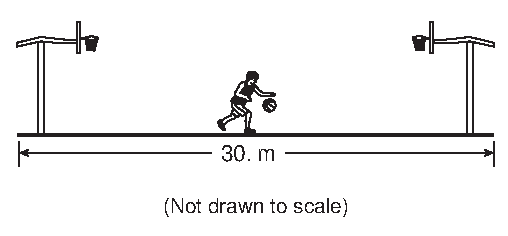
\includegraphics[keepaspectratio,scale=0.75]{June2012-Q01}
    \end{center}
    The magnitude of the player's total displacement after running the drill is:
    \begin{multicols}{2}
    \begin{choices}
      \correctchoice{\SI{0.0}{\meter}}
        \wrongchoice{\SI{30}{\meter}}
        \wrongchoice{\SI{60}{\meter}}
        \wrongchoice{\SI{180}{\meter}}
    \end{choices}
    \end{multicols}
\end{question}
}

\element{nysed}{
\begin{question}{June2012-Q02}
    In a drill during basketball practice,
        a player runs the length of the \SI{30}{\meter} court and back.
    The player does this three times in \SI{60}{\second}.
    \begin{center}
        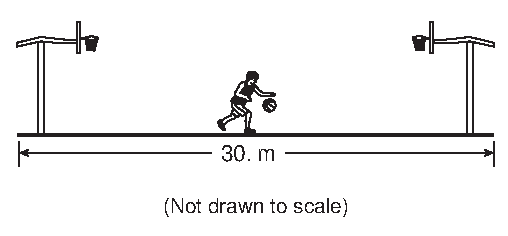
\includegraphics[keepaspectratio,scale=0.75]{June2012-Q01}
    \end{center}
    The average speed of the player during the drill is:
    \begin{multicols}{2}
    \begin{choices}
        \wrongchoice{\SI{0.0}{\meter\per\second}}
        \wrongchoice{\SI{0.50}{\meter\per\second}}
      \correctchoice{\SI{3.0}{\meter\per\second}}
        \wrongchoice{\SI{30}{\meter\per\second}}
    \end{choices}
    \end{multicols}
\end{question}
}


%% Section June2011
%%--------------------


%% Section June2010
%%--------------------
\element{nysed}{
\begin{question}{June2010-Q01}
    A baseball player runs \SI{27.4}{\meter} from the batter's box to first base,
        overruns first base by \SI{3.0}{\meter},
        and then returns to first base.
    Compared to the total distance traveled by the player,
        the magnitude of the player's total displacement from the batter's box is?
    \begin{multicols}{2}
    \begin{choices}
        \wrongchoice{\SI{3.0}{\meter} shorter}
      \correctchoice{\SI{6.0}{\meter} shorter}
        \wrongchoice{\SI{3.0}{\meter} longer}
        \wrongchoice{\SI{6.0}{\meter} longer}
    \end{choices}
    \end{multicols}
\end{question}
}


%% Section June2009
%%--------------------
\element{nysed}{
\begin{question}{June2009-Q01}
    On a highway, a car is driven \SI{80}{\kilo\meter} during the first \SI{1.00}{\hour} of travel,
        \SI{50}{\kilo\meter} during the next \SI{0.50}{\hour},
        and \SI{40}{\kilo\meter} in the final \SI{0.50}{\hour}.
    What is the car's average speed for the entire trip?
    \begin{multicols}{2}
    \begin{choices}
        \wrongchoice{\SI{45}{\kilo\meter\per\hour}}
        \wrongchoice{\SI{60}{\kilo\meter\per\hour}}
      \correctchoice{\SI{85}{\kilo\meter\per\hour}}
        \wrongchoice{\SI{170}{\kilo\meter\per\hour}}
    \end{choices}
    \end{multicols}
\end{question}
}

\element{nysed}{
\begin{question}{June2009-Q04}
    A high-speed train in Japan travels a distance of \SI{300}{\kilo\meter} in \SI{3.60e3}{\second}.
    What is the average speed of this train?
    \begin{multicols}{2}
    \begin{choices}
        \wrongchoice{\SI{1.20e-2}{\meter\per\second}}
        \wrongchoice{\SI{8.33e-2}{\meter\per\second}}
        \wrongchoice{\SI{12.0}{\meter\per\second}}
      \correctchoice{\SI{83.3}{\meter\per\second}}
    \end{choices}
    \end{multicols}
\end{question}
}


%% Section Jan2009
%%--------------------


%% Section June2008
%%--------------------
\element{nysed}{
\begin{question}{June2008-Q04}
    Approximately how much time does it take light to travel from Sun to Earth?
    \begin{multicols}{2}
    \begin{choices}
        \wrongchoice{\SI{2.00e-3}{\second}}
        \wrongchoice{\SI[retain-zero-exponent]{1.28e0}{\second}}
      \correctchoice{\SI{5.00e2}{\second}}
        \wrongchoice{\SI{4.50e19}{\second}}
    \end{choices}
    \end{multicols}
\end{question}
}


%% Section Jan2008
%%--------------------


%% Section June2007
%%--------------------


%% Section Jan2007
%%--------------------


%% Section June2006
%%--------------------


%% Section Jan2006
%%--------------------


%% Section June2005
%%--------------------


%% Section Jan2005
%%--------------------
\element{nysed}{
\begin{question}{Jan2005-Q02}
    In a \SI{4.0}{\kilo\meter} race, a runner completes the first kilometer in \SI{5.9}{\minute},
        the second kilometer in \SI{6.2}{\minute}, and the third kilometer in \SI{6.3}{\minute},
        and the final kilometer in \SI{6.0}{\minute}.
    The average speed of the runner for the race is approximately:
    \begin{multicols}{2}
    \begin{choices}
      \correctchoice{\SI{0.16}{\kilo\meter\per\minute}}
        \wrongchoice{\SI{0.33}{\kilo\meter\per\minute}}
        \wrongchoice{\SI{12}{\kilo\meter\per\minute}}
        \wrongchoice{\SI{24}{\kilo\meter\per\minute}}
    \end{choices}
    \end{multicols}
\end{question}
}


%% Section June2004
%%--------------------


%% Section Jan2004
%%--------------------


%% Section June2003
%%--------------------


%% Section Jan2003
%%--------------------


%% Section Aug2002
%%--------------------


%% Section June2002
%%--------------------


%% Section Jan2002
%%--------------------
\element{nysed}{
\begin{question}{Jan2002-Q03}
    A group of bike riders took a \SI{4.0}{\hour} trip.
    During the first \SI{3.0}{\hour},
        they traveled a total of \SI{50}{\kilo\meter},
        but during the last hour they traveled only \SI{10}{\kilo\meter}.
    What was the group's average speed for the entire trip?
    \begin{multicols}{2}
    \begin{choices}
      \correctchoice{\SI{15}{\kilo\meter\per\hour}}
        \wrongchoice{\SI{30}{\kilo\meter\per\hour}}
        \wrongchoice{\SI{40}{\kilo\meter\per\hour}}
        \wrongchoice{\SI{60}{\kilo\meter\per\hour}}
    \end{choices}
    \end{multicols}
\end{question}
}


%% Section June2001
%%--------------------
\element{nysed}{
\begin{question}{June2001-Q09}
    Two cars, $A$ and $B$, are \SI{400}{\meter} apart.
    Car $A$ travels due east at \SI{30}{\meter\per\second} on a collision course with car $B$,
        which travels due west at \SI{20}{\meter\per\second}.
    How much time elapses before the two cars collide?
    \begin{multicols}{2}
    \begin{choices}
      \correctchoice{\SI{8.0}{\second}}
        \wrongchoice{\SI{20}{\second}}
        \wrongchoice{\SI{13}{\second}}
        \wrongchoice{\SI{40}{\second}}
    \end{choices}
    \end{multicols}
\end{question}
}

\element{nysed}{
\begin{question}{June2001-Q53}
    A softball player leaves the batter's box,
        overruns first base by \SI{3.0}{\meter},
        and then returns to first base.
    Compared to the total distance traveled by the player,
        the magnitude of the player's total displacement from the batter's box is:
    \begin{multicols}{3}
    \begin{choices}
      \correctchoice{smaller}
        \wrongchoice{larger}
        \wrongchoice{the same}
    \end{choices}
    \end{multicols}
\end{question}
}


%% Section Jan2001
%%--------------------


%% Section June2000
%%--------------------


%% Section June1999
%%--------------------


%% Section June1998
%%--------------------
\element{nysed}{
\begin{question}{June1998-Q05}
    What is the average velocity of a car that travels \SI{30}{\kilo\meter} due west in \SI{0.50}{\hour}?
    \begin{multicols}{2}
    \begin{choices}
        \wrongchoice{\SI{15}{\kilo\meter\per\hour}}
        \wrongchoice{\SI{60}{\kilo\meter\per\hour}}
        \wrongchoice{\SI{15}{\kilo\meter\per\hour} west}
      \correctchoice{\SI{60}{\kilo\meter\per\hour} west}
    \end{choices}
    \end{multicols}
\end{question}
}


%% Section June1997
%%--------------------
\element{nysed}{
\begin{question}{June1997-Q02}
    A baseball pitcher throws a fastball at \SI{42}{\meter\per\second}.
    If the batter is \SI{18}{\meter} from the pitcher,
        approximately how much time does it take for the ball to reach the batter?
    \begin{multicols}{2}
    \begin{choices}
        \wrongchoice{\SI{1.0}{\second}}
        \wrongchoice{\SI{2.3}{\second}}
        \wrongchoice{\SI{0.86}{\second}}
      \correctchoice{\SI{0.43}{\second}}
    \end{choices}
    \end{multicols}
\end{question}
}


%% Section June1996
%%--------------------
\element{nysed}{
\begin{question}{June1996-Q01}
    A car travels between the \SI{100}{\meter} and \SI{250}{\meter} highway markers in \SI{10}{\second}.
    The average speed of the car during this interval is:
    \begin{multicols}{2}
    \begin{choices}
        \wrongchoice{\SI{10}{\meter\per\second}}
      \correctchoice{\SI{15}{\meter\per\second}}
        \wrongchoice{\SI{25}{\meter\per\second}}
        \wrongchoice{\SI{35}{\meter\per\second}}
    \end{choices}
    \end{multicols}
\end{question}
}


%% Section June1994
%%--------------------
\element{nysed}{
\begin{question}{June1994-Q44}
    The distance from the Moon to Earth is \SI{3.9e8}{\meter}.
    What is the time required for a light ray to travel from the Moon to Earth?
    \begin{multicols}{2}
    \begin{choices}
        \wrongchoice{\SI{0.65}{\second}}
      \correctchoice{\SI{1.3}{\second}}
        \wrongchoice{\SI{2.6}{\second}}
        \wrongchoice{\SI{3.9}{\second}}
    \end{choices}
    \end{multicols}
\end{question}
}


%% Section June1986
%%--------------------
\element{nysed}{
\begin{question}{June1986-Q02}
    The average speed of a plane was \SI{600}{\kilo\meter\per\hour}.
    How long did it take the plane to travel \SI{120}{\kilo\meter}?
    \begin{multicols}{2}
    \begin{choices}
      \correctchoice{\SI{0.2}{\hour}}
        \wrongchoice{\SI{0.5}{\hour}}
        \wrongchoice{\SI{0.7}{\hour}}
        \wrongchoice{\SI{5}{\hour}}
    \end{choices}
    \end{multicols}
\end{question}
}

\element{nysed}{
\begin{question}{June1986-Q19}
    It takes \SI{1}{\second} for a sound wave to travel from a source to observer $A$.
    How long does it take the same sound wave to travel in the same medium to observer $B$,
        who is located twice as far from the source as observer $A$?
    \begin{multicols}{4}
    \begin{choices}
        \wrongchoice{\SI{1/4}{\second}}
      \correctchoice{\SI{2}{\second}}
        \wrongchoice{\SI{1/2}{\second}}
        \wrongchoice{\SI{4}{\second}}
    \end{choices}
    \end{multicols}
\end{question}
}


%% Section June1985
%%--------------------
\element{nysed}{
\begin{question}{June1985-Q02}
    The distance-time graph below represents the position of an object moving in a straight line.
    \begin{center}
    \begin{tikzpicture}
        \begin{axis}[
            axis y line=left,
            axis x line=bottom,
            axis line style={->},
            xlabel={time},
            x unit=\si{\second},
            xtick={0,1,2,3,4,5,6},
            minor x tick num=1,
            ylabel={distance},
            y unit=\si{\meter},
            ytick={0,10,20,30},
            minor y tick num=1,
            xmin=0,xmax=6.3,
            ymin=0,ymax=31.5,
            width=0.8\columnwidth,
            height=0.5\columnwidth,
            grid=major,
            very thin,
        ]
        \addplot[line width=1pt,mark=\empty] plot coordinates { (0,0) (2,10) (4,30) (6,30)};
        \end{axis}
    \end{tikzpicture}
    \end{center}
    What is the speed of the object during the time interval $t=\SI{2.0}{\second}$ to $t=\SI{4.0}{\second}$?
    \begin{multicols}{2}
    \begin{choices}
        \wrongchoice{\SI{0.0}{\meter\per\second}}
        \wrongchoice{\SI{5.0}{\meter\per\second}}
        \wrongchoice{\SI{7.5}{\meter\per\second}}
      \correctchoice{\SI{10.}{\meter\per\second}}
    \end{choices}
    \end{multicols}
\end{question}
}



\endinput



%
%% Constant Accleration Questions
%% NYSED Physics Regents Examination
%%--------------------------------------------------

%% this section contains 59 problems


%% Section June2015
%%--------------------
\element{nysed}{
\begin{question}{June2015-Q40}
    A car, initially traveling at \SI{15}{\meter\per\second} north,
        accelerates to \SI{25}{\meter\per\second} north in \SI{4.0}{\second}.
    The magnitude of the average acceleration is:
    \begin{multicols}{2}
    \begin{choices}
      \correctchoice{\SI{2.5}{\meter\per\second\squared}}
        \wrongchoice{\SI{6.3}{\meter\per\second\squared}}
        \wrongchoice{\SI{10.}{\meter\per\second\squared}}
        \wrongchoice{\SI{20.}{\meter\per\second\squared}}
    \end{choices}
    \end{multicols}
\end{question}
}


%% Section June2014
%%--------------------
\element{nysed}{
\begin{question}{June2014-Q02}
    What is the final speed of an object that starts from rest and accelerates uniformly at \SI{4.0}{\meter\per\second\squared} over a distance of \SI{8.0}{\meter}?
    \begin{multicols}{2}
    \begin{choices}
      \correctchoice{\SI{8.0}{\meter\per\second}}
        \wrongchoice{\SI{16}{\meter\per\second}}
        \wrongchoice{\SI{32}{\meter\per\second}}
        \wrongchoice{\SI{64}{\meter\per\second}}
    \end{choices}
    \end{multicols}
\end{question}
}

\element{nysed}{
\begin{question}{June2014-Q07}
    A truck, initially traveling at a speed of \SI{22}{\meter\per\second},
        increases speed at a constant rate of \SI{2.4}{\meter\per\second\squared} for \SI{3.2}{\second}.
    What is the total distance traveled by the truck during this \SI{3.2}{\second} time interval?
    \begin{multicols}{2}
    \begin{choices}
      \correctchoice{\SI{83}{\meter}}
        \wrongchoice{\SI{70.}{\meter}}
        \wrongchoice{\SI{12}{\meter}}
        \wrongchoice{\SI{58}{\meter}}
    \end{choices}
    \end{multicols}
\end{question}
}


%% Section June2013
%%--------------------
\element{nysed}{
\begin{question}{June2013-Q03}
    A car traveling west in a straight line on a highway decreases its speed from \SI{30.0}{\meter\per\second} to \SI{23.0}{\meter\per\second} in \SI{2.00}{\second}.
    The car's average acceleration during this time interval is:
    \begin{multicols}{2}
    \begin{choices}
      \correctchoice{\SI{3.5}{\meter\per\second\squared} east}
        \wrongchoice{\SI{3.5}{\meter\per\second\squared} west}
        \wrongchoice{\SI{13}{\meter\per\second\squared} east}
        \wrongchoice{\SI{13}{\meter\per\second\squared} west}
    \end{choices}
    \end{multicols}
\end{question}
}

\element{nysed}{
\begin{question}{June2013-Q04}
    In a race, a runner traveled \SI{12}{\meter} in \SI{4.0}{\second} as she accelerated uniformly from rest.
    The magnitude of the acceleration of the runner was:
    \begin{multicols}{2}
    \begin{choices}
        \wrongchoice{\SI{0.25}{\meter\per\second\squared}}
      \correctchoice{\SI{1.5}{\meter\per\second\squared}}
        \wrongchoice{\SI{3.0}{\meter\per\second\squared}}
        \wrongchoice{\SI{48}{\meter\per\second\squared}}
    \end{choices}
    \end{multicols}
\end{question}
}


%% Section June2012
%%--------------------
\element{nysed}{
\begin{question}{June2012-Q06}
    A car, initially traveling east with a speed of \SI{5.0}{\meter\per\second},
        is accelerated uniformly at \SI{2.0}{\meter\per\second\squared} east for \SI{10}{\second} along a straight line.
    During this \SI{10}{\second} interval the car travels a total distance of:
    \begin{multicols}{2}
    \begin{choices}
        \wrongchoice{\SI{50}{\meter}}
        \wrongchoice{\SI{60}{\meter}}
        \wrongchoice{\SI{1.0e2}{\meter}}
      \correctchoice{\SI{1.5e2}{\meter}}
    \end{choices}
    \end{multicols}
\end{question}
}

\element{nysed}{
\begin{question}{June2012-Q08}
    A child riding a bicycle at \SI{15}{\meter\per\second} accelerates at \SI{-3.0}{\meter\per\second\squared} for \SI{4.0}{\second}.
    What is the child's speed at the end of this \SI{4.0}{\second} interval?
    \begin{multicols}{2}
    \begin{choices}
        \wrongchoice{\SI{12}{\meter\per\second}}
        \wrongchoice{\SI{27}{\meter\per\second}}
      \correctchoice{\SI{3.0}{\meter\per\second}}
        \wrongchoice{\SI{7.0}{\meter\per\second}}
    \end{choices}
    \end{multicols}
\end{question}
}


%% Section June2011
%%--------------------
\element{nysed}{
\begin{question}{June2011-Q02}
    If a car accelerates uniformly from rest to \SI{15}{\meter\per\second} over a distance of \SI{100}{\meter},
        the magnitude of a car's acceleration is:
    \begin{multicols}{2}
    \begin{choices}
        \wrongchoice{\SI{0.15}{\meter\per\second\squared}}
      \correctchoice{\SI{1.1}{\meter\per\second\squared}}
        \wrongchoice{\SI{2.3}{\meter\per\second\squared}}
        \wrongchoice{\SI{6.7}{\meter\per\second\squared}}
    \end{choices}
    \end{multicols}
\end{question}
}

\element{nysed}{
\begin{question}{June2011-Q03}
    An object accelerates uniformly from \SI{3.0}{\meter\per\second} east to \SI{8.0}{\meter\per\second} east in \SI{2.0}{\second}.
    What is the magnitude of the acceleration of the object?
    \begin{multicols}{2}
    \begin{choices}
      \correctchoice{\SI{2.5}{\meter\per\second\squared}}
        \wrongchoice{\SI{5.0}{\meter\per\second\squared}}
        \wrongchoice{\SI{5.5}{\meter\per\second\squared}}
        \wrongchoice{\SI{11}{\meter\per\second\squared}}
    \end{choices}
    \end{multicols}
\end{question}
}

\element{nysed}{
\begin{question}{June2011-Q04}
    A rock is dropped from a bridge.
    What happens to the magnitude of the acceleration and the speed of the rock as it falls?
    [Neglect friction.]
    \begin{choices}
        \wrongchoice{Both acceleration and speed increase.}
        \wrongchoice{Both acceleration and speed remain the same.}
        \wrongchoice{Acceleration increases and speed decreases.}
      \correctchoice{Acceleration remains the same and speed increases.}
    \end{choices}
\end{question}
}

\element{nysed}{
\begin{question}{June2011-Q05}
    A soccer ball is kicked on a level field has an initial vertical velocity component of \SI{15.0}{\meter\per\second}.
    Assuming the ball lands at the same height from which it was kicked,
        what is the total time the ball is in the air?
    [Neglect friction.]
    \begin{multicols}{2}
    \begin{choices}
        \wrongchoice{\SI{0.654}{\second}}
        \wrongchoice{\SI{1.53}{\second}}
      \correctchoice{\SI{3.06}{\second}}
        \wrongchoice{\SI{6.12}{\second}}
    \end{choices}
    \end{multicols}
\end{question}
}

\element{nysed}{
\begin{question}{June2011-Q37}
    The graph below shows the relationship between the speed and elapsed time for an object falling freely from rest near the surface of a planet.
    \begin{center}
    \begin{tikzpicture}
        \begin{axis}[
            axis y line=left,
            axis x line=bottom,
            axis line style={->},
            xlabel={Time},
            x unit=\si{\second},
            xtick={0.0,1.0,2.0,3.0,4.0},
            ylabel={Speed},
            y unit=\si{\meter\per\second},
            ytick={0.0,2.0,4.0,6.0,8.0,10.0},
            xmin=0,xmax=4,
            ymin=0,ymax=10,
            grid=major,
            width=0.8\columnwidth,
            height=0.5\columnwidth,
            very thin,
        ]
        \addplot[line width=1pt,domain=0:4]{8*x/3};
        \end{axis}
    \end{tikzpicture}
    \end{center}
    What is the total distance the object falls during
        the first \SI{3.0}{\second}?
    \begin{multicols}{2}
    \begin{choices}
      \correctchoice{\SI{12}{\meter}}
        \wrongchoice{\SI{24}{\meter}}
        \wrongchoice{\SI{44}{\meter}}
        \wrongchoice{\SI{72}{\meter}}
    \end{choices}
    \end{multicols}
\end{question}
}


%% Section June2010
%%--------------------
\element{nysed}{
\begin{question}{June2010-Q03}
    A car traveling on a straight road at \SI{15.0}{\meter\per\second} accelerates uniformly to a speed of \SI{21.0}{\meter\per\second} in \SI{12.0}{\second}.
    The total distance traveled by the car in this \SI{12.0}{\second} time interval is:
    \begin{multicols}{2}
    \begin{choices}
        \wrongchoice{\SI{36.0}{\meter}}
        \wrongchoice{\SI{180}{\meter}}
      \correctchoice{\SI{216}{\meter}}
        \wrongchoice{\SI{252}{\meter}}
    \end{choices}
    \end{multicols}
\end{question}
}


%% Section June2009
%%--------------------
\newcommand{\myJuneZeroNineQthirtySevenTikz}{
    \begin{tikzpicture}
        \begin{axis}[
            axis y line=left,
            axis x line=bottom,
            axis line style={->},
            xlabel={time},
            x unit=\si{\second},
            xtick={0,2,4,6},
            ylabel={velocity},
            y unit=\si{\meter\per\second},
            ytick={0,5,10,15},
            xmin=0,xmax=6.5,
            ymin=0,ymax=16,
            grid=major,
            width=0.8\columnwidth,
            height=0.5\columnwidth,
            very thin,
        ]
        \addplot[line width=1pt,domain=0:4]{2.5*x};
        \addplot[line width=1pt,domain=4:6]{10};
        \end{axis}
    \end{tikzpicture}
}

\element{nysed}{
\begin{question}{June2009-Q37}
    The diagram below represents the motion of a car during a \SI{6.0}{\second} time interval.
    \begin{center}
        \myJuneZeroNineQthirtySevenTikz
    \end{center}
    What is the acceleration of the car at $t=\SI{5.0}{\second}$?
    \begin{multicols}{2}
    \begin{choices}
      \correctchoice{\SI{0.0}{\meter\per\second\squared}}
        \wrongchoice{\SI{2.0}{\meter\per\second\squared}}
        \wrongchoice{\SI{2.5}{\meter\per\second\squared}}
        \wrongchoice{\SI{10.0}{\meter\per\second\squared}}
    \end{choices}
    \end{multicols}
\end{question}
}

\element{nysed}{
\begin{question}{June2009-Q38}
    The diagram below represents the motion of a car during a \SI{6.0}{\second} time interval.
    \begin{center}
        \myJuneZeroNineQthirtySevenTikz
    \end{center}
    What is the total distance traveled by the car during this \SI{6.0}{\second} interval?
    \begin{multicols}{2}
    \begin{choices}
        \wrongchoice{\SI{10.}{\meter}}
        \wrongchoice{\SI{20.}{\meter}}
      \correctchoice{\SI{40.}{\meter}}
        \wrongchoice{\SI{60.}{\meter}}
    \end{choices}
    \end{multicols}
\end{question}
}


%% Section Jan2009
%%--------------------
\element{nysed}{
\begin{question}{Jan2009-Q04}
    As a car driven south in a straight line with \emph{decreasing} speed,
        the acceleration of the car must be:
    \begin{choices}
      \correctchoice{directed northward}
        \wrongchoice{directed southward}
        \wrongchoice{zero}
        \wrongchoice{constant, but not zero}
    \end{choices}
\end{question}
}


%% Section June2008
%%--------------------
\element{nysed}{
\begin{question}{June2008-Q07}
    The speed of an object undergoing constant acceleration increases from \SI{8.0}{\meter\per\second} to \SI{16.0}{\meter\per\second} in \SI{10}{\second}.
    How far does the object travel during the \SI{10}{\second}?
    \begin{multicols}{2}
    \begin{choices}
        \wrongchoice{\SI{3.6e2}{\meter}}
        \wrongchoice{\SI{1.6e2}{\meter}}
      \correctchoice{\SI{1.2e2}{\meter}}
        \wrongchoice{\SI{8.0e1}{\meter}}
    \end{choices}
    \end{multicols}
\end{question}
}

\element{nysed}{
\begin{question}{June2008-Q37}
    The graph below represents the displacement of an object moving in a straight line as a function of time.
    \begin{center}
    \begin{tikzpicture}
        \begin{axis}[
            axis y line=left,
            axis x line=bottom,
            axis line style={->},
            xlabel={Time},
            x unit=\si{\second},
            xtick={0.0,2.0,4.0,6.0,8.0,10,0},
            ylabel={displacement},
            y unit=\si{\meter},
            ytick={0,4,8,12,16},
            xmin=0,xmax=10,
            ymin=0,ymax=16,
            grid=major,
            width=0.8\columnwidth,
            height=0.5\columnwidth,
            very thin,
        ]
        \addplot[line width=1pt,domain=0:4]{2*x};
        \addplot[line width=1pt,domain=4:6]{8};
        \addplot[line width=1pt,domain=6:10]{ 8 - 2*( (x-6) * (x-10) )};
        \end{axis}
    \end{tikzpicture}
    \end{center}
    What was the total distance traveled by the object during the \SI{10}{\second} time interval?
    \begin{multicols}{2}
    \begin{choices}
        \wrongchoice{\SI{0}{\meter}}
        \wrongchoice{\SI{8}{\meter}}
        \wrongchoice{\SI{16}{\meter}}
      \correctchoice{\SI{24}{\meter}}
    \end{choices}
    \end{multicols}
\end{question}
}


%% Section Jan2008
%%--------------------
\element{nysed}{
\begin{question}{Jan2008-Q02}
    A race car starting from rest accelerates uniformly at a rate of \SI{4.9}{\meter\per\second\squared}.
    What is the car's speed after it has traveled \SI{200}{\meter}.
    \begin{multicols}{2}
    \begin{choices}
      \correctchoice{\SI{44.3}{\meter\per\second}}
        \wrongchoice{\SI{62.6}{\meter\per\second}}
        \wrongchoice{\SI{1960}{\meter\per\second}}
        \wrongchoice{\SI{31.3}{\meter\per\second}}
    \end{choices}
    \end{multicols}
\end{question}
}


%% Section June2007
%%--------------------
\element{nysed}{
\begin{question}{June2007-Q02}
    An astronaut standing on a platform on the Moon drops a hammer.
    If the hammer falls \SI{6.0}{\meter} vertically in \SI{2.7}{\second},
        what is the acceleration?
    \begin{multicols}{2}
    \begin{choices}
      \correctchoice{\SI{1.6}{\meter\per\second\squared}}
        \wrongchoice{\SI{2.2}{\meter\per\second\squared}}
        \wrongchoice{\SI{4.4}{\meter\per\second\squared}}
        \wrongchoice{\SI{9.8}{\meter\per\second\squared}}
    \end{choices}
    \end{multicols}
\end{question}
}

\element{nysed}{
\begin{question}{June2007-Q40}
    An observer recorded the following data for the motion of a car undergoing constant acceleration.
    \begin{center}
    \begin{tabu}{cc}
        Time (\si{\second}) & Speed (\si{\meter\per\second}) \\
        \midrule
        3.0 & 4.0 \\
        5.0 & 7.0 \\
        6.0 & 8.5 \\
    \end{tabu}
    \end{center}
    What was the magnitude of the acceleration of the car?
    \begin{multicols}{2}
    \begin{choices}
        \wrongchoice{\SI{1.3}{\meter\per\second\squared}}
        \wrongchoice{\SI{2.0}{\meter\per\second\squared}}
      \correctchoice{\SI{1.5}{\meter\per\second\squared}}
        \wrongchoice{\SI{4.5}{\meter\per\second\squared}}
    \end{choices}
    \end{multicols}
\end{question}
}


%% Section Jan2007
%%--------------------
\element{nysed}{
\begin{question}{Jan2007-Q03}
    A car increases its speed from \SI{9.6}{\meter\per\second} to \SI{11.2}{\meter\per\second} in \SI{4.0}{\second}.
    The average acceleration of the car during this \SI{4.0}{\second} interval is:
    \begin{multicols}{2}
    \begin{choices}
      \correctchoice{\SI{0.40}{\meter\per\second\squared}}
        \wrongchoice{\SI{2.4}{\meter\per\second\squared}}
        \wrongchoice{\SI{2.8}{\meter\per\second\squared}}
        \wrongchoice{\SI{5.2}{\meter\per\second\squared}}
    \end{choices}
    \end{multicols}
\end{question}
}

\element{nysed}{
\begin{question}{Jan2007-Q36}
    A cart travels with a constant nonzero acceleration along a straight line.
    Which graph best represents the relationship between the distance the cart travels and the time of travel?
    \begin{multicols}{2}
    \begin{choices}
        \AMCboxDimensions{down=-2.5em}
        \correctchoice{
            \begin{tikzpicture}
                \begin{axis}[
                    axis y line=left,
                    axis x line=bottom,
                    axis line style={->},
                    xlabel={time},
                    xtick=\empty,
                    ylabel={distance},
                    ytick=\empty,
                    xmin=0,xmax=11,
                    ymin=0,ymax=11,
                    width=\columnwidth,
                    very thin,
                ]
                \addplot[line width=1pt,domain=0:10]{0.1 * x*x};
                \end{axis}
            \end{tikzpicture}
        }
        \wrongchoice{
            \begin{tikzpicture}
                \begin{axis}[
                    axis y line=left,
                    axis x line=bottom,
                    axis line style={->},
                    xlabel={time},
                    xtick=\empty,
                    ylabel={distance},
                    ytick=\empty,
                    xmin=0,xmax=11,
                    ymin=0,ymax=11,
                    width=\columnwidth,
                    very thin,
                ]
                \addplot[line width=1pt,domain=0:10]{10-x};
                \end{axis}
            \end{tikzpicture}
        }
        \wrongchoice{
            \begin{tikzpicture}
                \begin{axis}[
                    axis y line=left,
                    axis x line=bottom,
                    axis line style={->},
                    xlabel={time},
                    xtick=\empty,
                    ylabel={distance},
                    ytick=\empty,
                    xmin=0,xmax=185,
                    ymin=0,ymax=10,
                    width=\columnwidth,
                    very thin,
                ]
                \addplot[line width=1pt,domain=0:180]{8*sin(x)};
                \end{axis}
            \end{tikzpicture}
        }
        \wrongchoice{
            \begin{tikzpicture}
                \begin{axis}[
                    axis y line=left,
                    axis x line=bottom,
                    axis line style={->},
                    xlabel={time},
                    xtick=\empty,
                    ylabel={distance},
                    ytick=\empty,
                    xmin=0,xmax=11,
                    ymin=0,ymax=11,
                    width=\columnwidth,
                    very thin,
                ]
                \addplot[line width=1pt,domain=0:10]{x};
                \end{axis}
            \end{tikzpicture}
        }
    \end{choices}
    \end{multicols}
\end{question}
}


%% Section June2006
%%--------------------
\element{nysed}{
\begin{question}{June2006-Q02}
    A rocket initially at rest on the ground lifts off vertically with a constant acceleration of \SI{2.0e1}{\meter\per\second\squared}.
    How long will it take the rocket to reach an altitude of \SI{9.0e3}{\meter}?
    \begin{multicols}{2}
    \begin{choices}
      \correctchoice{\SI{3.0e1}{\second}}
        \wrongchoice{\SI{4.3e1}{\second}}
        \wrongchoice{\SI{4.5e2}{\second}}
        \wrongchoice{\SI{9.0e2}{\second}}
    \end{choices}
    \end{multicols}
\end{question}
}


%% Section Jan2006
%%--------------------
\element{nysed}{
\begin{question}{Jan2006-Q01}
    The speed of a wagon increases from \SI{2.5}{\meter\per\second} to \SI{9.0}{\meter\per\second} in \SI{3.0}{\second} as it accelerates uniformly down a hill.
    what is the magnitude of the acceleration of the wagon during this \SI{3.0}{\second} interval?
    \begin{multicols}{2}
    \begin{choices}
        \wrongchoice{\SI{0.83}{\meter\per\second\squared}}
      \correctchoice{\SI{2.2}{\meter\per\second\squared}}
        \wrongchoice{\SI{3.0}{\meter\per\second\squared}}
        \wrongchoice{\SI{3.8}{\meter\per\second\squared}}
    \end{choices}
    \end{multicols}
\end{question}
}

\element{nysed}{
\begin{question}{Jan2006-Q38}
    The graph below represents the relationship between speed and time for an object moving along a straight line.
    \begin{center}
    \begin{tikzpicture}
        \begin{axis}[
            axis y line=left,
            axis x line=bottom,
            axis line style={->},
            title={Speed vs. Time},
            xlabel={time},
            xtick={0,1,2,3,4,5},
            x unit=\si{\second},
            ylabel={speed},
            y unit=\si{\meter\per\second},
            ytick={0,5,10,15,20,25},
            xmin=0,xmax=5,
            ymin=0,ymax=25,
            grid=major,
            width=0.8\columnwidth,
            height=0.5\columnwidth,
            very thin,
        ]
        \addplot[line width=1pt,domain=0:5]{5*x};
        \end{axis}
    \end{tikzpicture}
    \end{center}
    What is the total distance traveled by the object during the first \SI{4}{\second}?
    \begin{multicols}{2}
    \begin{choices}
        \wrongchoice{\SI{5}{\meter}}
        \wrongchoice{\SI{20}{\meter}}
      \correctchoice{\SI{40}{\meter}}
        \wrongchoice{\SI{80}{\meter}}
    \end{choices}
    \end{multicols}
\end{question}
}


%% Section Jan2005
%%--------------------
\element{nysed}{
\begin{question}{Jan2005-Q36}
    Which pair of graphs represents the same motion of an object?
    \begin{choices}
        \AMCboxDimensions{down=-2.5em}
        \correctchoice{
            \begin{tikzpicture}
                \begin{groupplot}[
                        axis y line=left,
                        axis x line=bottom,
                        axis line style={->},
                        group style={group size=2 by 1},
                        xtick=\empty,
                        ytick=\empty,
                        width=0.5\columnwidth,
                    ]
                    \nextgroupplot[
                        xlabel={time},
                        ylabel={displacement},
                        xmin=0,xmax=11,
                        ymin=0,ymax=11,
                    ] \addplot[line width=1pt,domain=0:10] {0.1*x*x};
                    \nextgroupplot[
                        xlabel={time},
                        ylabel={velocity},
                        xmin=0,xmax=11,
                        ymin=0,ymax=11,
                    ] \addplot[line width=1pt,domain=0:10] {x};
                \end{groupplot}
            \end{tikzpicture}
        }
        \wrongchoice{
            \begin{tikzpicture}
                \begin{groupplot}[
                        axis y line=left,
                        axis x line=middle,
                        axis line style={->},
                        group style={group size=2 by 1},
                        xtick=\empty,
                        ytick=\empty,
                        width=0.5\columnwidth,
                    ]
                    \nextgroupplot[
                        xlabel={time},
                        ylabel={displacement},
                        x label style={anchor=north east},
                        xmin=0,xmax=11,
                        ymin=-5.5,ymax=5.5,
                    ] \addplot[line width=1pt,domain=0:10] {-5+x};
                    \nextgroupplot[
                        xlabel={time},
                        ylabel={velocity},
                        xmin=0,xmax=11,
                        ymin=-5.5,ymax=5.5,
                    ] \addplot[line width=1pt,domain=0:10] {-3};
                \end{groupplot}
            \end{tikzpicture}
        }
        \wrongchoice{
            \begin{tikzpicture}
                \begin{groupplot}[
                        axis y line=left,
                        axis x line=middle,
                        axis line style={->},
                        group style={group size=2 by 1},
                        xtick=\empty,
                        ytick=\empty,
                        width=0.5\columnwidth,
                    ]
                    \nextgroupplot[
                        xlabel={time},
                        ylabel={displacement},
                        xmin=0,xmax=11,
                        ymin=-5.5,ymax=5.5,
                    ] \addplot[line width=1pt,domain=0:10] {5-x};
                    \nextgroupplot[
                        xlabel={time},
                        ylabel={velocity},
                        x label style={anchor=north east},
                        xmin=0,xmax=11,
                        ymin=-5.5,ymax=5.5,
                    ] \addplot[line width=1pt,domain=0:10] {-5+x};
                \end{groupplot}
            \end{tikzpicture}
        }
        \wrongchoice{
            \begin{tikzpicture}
                \begin{groupplot}[
                        axis y line=left,
                        axis x line=bottom,
                        axis line style={->},
                        group style={group size=2 by 1},
                        xtick=\empty,
                        ytick=\empty,
                        width=0.5\columnwidth,
                    ]
                    \nextgroupplot[
                        xlabel={time},
                        ylabel={displacement},
                        xmin=0,xmax=11,
                        ymin=0,ymax=11,
                    ] \addplot[line width=1pt,domain=0:10] {-0.4 *x * (x-10)};
                    \nextgroupplot[
                        xlabel={time},
                        ylabel={velocity},
                        xmin=0,xmax=11,
                        ymin=0,ymax=11,
                    ] \addplot[line width=1pt,domain=0:10] {8};
                \end{groupplot}
            \end{tikzpicture}
        }
    \end{choices}
\end{question}
}



%% Section Jan2004
%%--------------------
\element{nysed}{
\begin{question}{Jan2004-Q03}
    A skater increases her speed uniformly from \SI{2.0}{\meter\per\second}
        to \SI{7.0}{\meter\per\second} over a distance of \SI{12}{\meter}.
    The magnitude of her acceleration as she travels this \SI{12}{\meter} is:
    \begin{multicols}{2}
    \begin{choices}
      \correctchoice{\SI{1.9}{\meter\per\second\squared}}
        \wrongchoice{\SI{2.2}{\meter\per\second\squared}}
        \wrongchoice{\SI{2.4}{\meter\per\second\squared}}
        \wrongchoice{\SI{3.8}{\meter\per\second\squared}}
    \end{choices}
    \end{multicols}
\end{question}
}


%% Section June2003
%%--------------------
\element{nysed}{
\begin{question}{June2003-Q03}
    A car initially traveling at a speed of \SI{16}{\meter\per\second} accelerates uniformly to a speed of \SI{20}{\meter\per\second} over a distance of \SI{36}{\meter}.
    What is the magnitude of the car's acceleration?
    \begin{multicols}{2}
    \begin{choices}
      \correctchoice{\SI{2.0}{\meter\per\second\squared}}
        \wrongchoice{\SI{0.22}{\meter\per\second\squared}}
        \wrongchoice{\SI{9.0}{\meter\per\second\squared}}
        \wrongchoice{\SI{0.11}{\meter\per\second\squared}}
    \end{choices}
    \end{multicols}
\end{question}
}


%% Section Jan2003
%%--------------------

\element{nysed}{
\begin{question}{Jan2003-Q45}
    Which graph best represents the motion of a block accelerating uniformly down an inclined plane?
    \begin{multicols}{2}
    \begin{choices}
        \AMCboxDimensions{down=-2.5em}
        \correctchoice{
            \begin{tikzpicture}
                \begin{axis}[
                    axis y line=left,
                    axis x line=bottom,
                    axis line style={->},
                    xlabel={time},
                    xtick=\empty,
                    ylabel={distance},
                    ytick=\empty,
                    xmin=0,xmax=11,
                    ymin=0,ymax=11,
                    width=\columnwidth,
                    very thin,
                ]
                \addplot[line width=1pt,domain=0:10]{0.1*x*x};
                \end{axis}
            \end{tikzpicture}
        }
        \wrongchoice{
            \begin{tikzpicture}
                \begin{axis}[
                    axis y line=left,
                    axis x line=bottom,
                    axis line style={->},
                    xlabel={time},
                    xtick=\empty,
                    ylabel={distance},
                    ytick=\empty,
                    xmin=0,xmax=11,
                    ymin=0,ymax=11,
                    width=\columnwidth,
                    very thin,
                ]
                \addplot[line width=1pt,domain=0:10]{x};
                \end{axis}
            \end{tikzpicture}
        }
        \wrongchoice{
            \begin{tikzpicture}
                \begin{axis}[
                    axis y line=left,
                    axis x line=bottom,
                    axis line style={->},
                    xlabel={time},
                    xtick=\empty,
                    ylabel={distance},
                    ytick=\empty,
                    xmin=0,xmax=11,
                    ymin=0,ymax=11,
                    width=\columnwidth,
                    very thin,
                ]
                \addplot[line width=1pt,domain=0:10]{7};
                \end{axis}
            \end{tikzpicture}
        }
        \wrongchoice{
            \begin{tikzpicture}
                \begin{axis}[
                    axis y line=left,
                    axis x line=bottom,
                    axis line style={->},
                    xlabel={time},
                    xtick=\empty,
                    ylabel={distance},
                    ytick=\empty,
                    xmin=0,xmax=11,
                    ymin=0,ymax=11,
                    width=\columnwidth,
                    very thin,
                ]
                \addplot[line width=1pt,domain=0:5]{1+1.2*x};
                \addplot[line width=1pt,domain=5:10]{7};
                \end{axis}
            \end{tikzpicture}
        }
    \end{choices}
    \end{multicols}
\end{question}
}


%% Section Aug2002
%%--------------------
\element{nysed}{
\begin{question}{Aug2002-Q02}
    The speed of a car is increased uniformly from \SI{20}{\meter\per\second} to \SI{30}{\meter\per\second} in \SI{4.0}{\second}.
    The magnitude of the car's average acceleration in this \SI{4.0}{\second} interval is:
    \begin{multicols}{2}
    \begin{choices}
        \wrongchoice{\SI{0.40}{\meter\per\second\squared}}
      \correctchoice{\SI{2.5}{\meter\per\second\squared}}
        \wrongchoice{\SI{10}{\meter\per\second\squared}}
        \wrongchoice{\SI{13}{\meter\per\second\squared}}
    \end{choices}
    \end{multicols}
\end{question}
}

\element{nysed}{
\begin{question}{Aug2002-Q03}
    A roller coaster, traveling with an initial speed of \SI{15}{\meter\per\second},
        decelerates uniformly at \SI{-7.0}{\meter\per\second\squared} to a full stop.
    Approximately how far does the roller coaster travel during its deceleration?
    \begin{multicols}{2}
    \begin{choices}
        \wrongchoice{\SI{1.0}{\meter}}
        \wrongchoice{\SI{2.0}{\meter}}
      \correctchoice{\SI{16}{\meter}}
        \wrongchoice{\SI{32}{\meter}}
    \end{choices}
    \end{multicols}
\end{question}
}

\element{nysed}{
\begin{question}{Aug2002-Q39}
    The graph below shows the velocity of a race car moving along a straight line as a function of time.
    \begin{center}
    \begin{tikzpicture}
        \begin{axis}[
            clip=false,
            axis y line=left,
            axis x line=bottom,
            axis line style={->},
            xlabel={time},
            x unit=\si{\second},
            xtick={0,1,2,3,4},
            ylabel={velocity},
            y unit=\si{\meter\per\second},
            ytick={0,10,20,30,40},
            xmin=0,xmax=4.1,
            ymin=0,ymax=42,
            grid=major,
            width=0.8\columnwidth,
            height=0.5\columnwidth,
            very thin,
        ]
        \addplot[line width=1pt,domain=0:4]{10*x};
        \end{axis}
    \end{tikzpicture}
    \end{center}
    What is the magnitude of the displacement of the car from $t=\SI{2.0}{\second}$ to $t=\SI{4.0}{\second}$?
    \begin{multicols}{2}
    \begin{choices}
        \wrongchoice{\SI{20}{\meter}}
        \wrongchoice{\SI{40}{\meter}}
      \correctchoice{\SI{60}{\meter}}
        \wrongchoice{\SI{80}{\meter}}
    \end{choices}
    \end{multicols}
\end{question}
}


%% Section June2002
%%--------------------
\element{nysed}{
\begin{question}{June2002-Q03}
    An object with an initial speed of \SI{4.0}{\meter\per\second} accelerates uniformly at \SI{2.0}{\meter\per\second\squared} in the direction of its motion for a distance of \SI{5.0}{\meter}.
    What is the final speed of the object?
    \begin{multicols}{2}
    \begin{choices}
      \correctchoice{\SI{6.0}{\meter\per\second}}
        \wrongchoice{\SI{10}{\meter\per\second}}
        \wrongchoice{\SI{14}{\meter\per\second}}
        \wrongchoice{\SI{36}{\meter\per\second}}
    \end{choices}
    \end{multicols}
\end{question}
}

\element{nysed}{
\begin{question}{June2002-Q04}
    After a model rocket reached its maximum height, it then took \SI{5.0}{\second} to return to the launch site.
    What is the approximate maximum height reached by the rocket?
    [Neglect air resistance]
    \begin{multicols}{2}
    \begin{choices}
        \wrongchoice{\SI{49}{\meter}}
        \wrongchoice{\SI{98}{\meter}}
      \correctchoice{\SI{120}{\meter}}
        \wrongchoice{\SI{250}{\meter}}
    \end{choices}
    \end{multicols}
\end{question}
}

\element{nysed}{
\begin{question}{June2002-Q36}
    The displacement-time graph below represents the motion of a cart initially moving in a straight line.
    \begin{center}
    \begin{tikzpicture}
        \begin{axis}[
            clip=false,
            axis y line=left,
            axis x line=bottom,
            axis line style={->},
            xlabel={time},
            xtick=\empty,
            ylabel={displacement},
            ytick=\empty,
            xmin=0,xmax=26,
            ymin=0,ymax=12,
            width=0.8\columnwidth,
            height=0.5\columnwidth,
            very thin,
        ]
        \addplot[line width=1pt,domain=0:5]{0.24*x*x}
            node[black,pos=0,anchor=north] {$A$};
        \addplot[line width=1pt,domain=5:14]{6 + (x-5)/3}
            node[black,pos=0,anchor=south] {$B$};
        \addplot[line width=1pt,domain=14:20]{9}
            node[black,pos=0,anchor=south] {$C$};
        \addplot[line width=1pt,domain=20:24]{9 - 1.25*(x-20)}
            node[black,pos=0,anchor=south west] {$D$}
            node[black,pos=1,anchor=west] {$E$};
        \addplot[only marks,mark=*,mark size=2pt] coordinates
            { (0,0) (5,6) (14,9) (20,9) (24,4) };
        \end{axis}
    \end{tikzpicture}
    \end{center}
    During which interval is the cart moving forward at constant speed?
    \begin{multicols}{2}
    \begin{choices}
        \wrongchoice{$AB$}
      \correctchoice{$BC$}
        \wrongchoice{$CD$}
        \wrongchoice{$DE$}
    \end{choices}
    \end{multicols}
\end{question}
}


%% Section Jan2002
%%--------------------
\element{nysed}{
\begin{question}{Jan2002-Q04}
    A skier starting from rest skis straight down a slope \SI{50}{\meter} long in \SI{5.0}{\second}.
    What is the magnitude of the acceleration of the skier?
    \begin{multicols}{2}
    \begin{choices}
        \wrongchoice{\SI{20}{\meter\per\second\squared}}
        \wrongchoice{\SI{9.8}{\meter\per\second\squared}}
        \wrongchoice{\SI{5.0}{\meter\per\second\squared}}
      \correctchoice{\SI{4.0}{\meter\per\second\squared}}
    \end{choices}
    \end{multicols}
\end{question}
}


%% Section June2001
%%--------------------
\element{nysed}{
\begin{question}{June2001-Q03}
    Which graph best represents the motion of an object whose speed is increasing?
    \begin{multicols}{2}
    \begin{choices}
        \AMCboxDimensions{down=-2.5em}
        \correctchoice{
            \begin{tikzpicture}
                \begin{axis}[
                    axis y line=left,
                    axis x line=bottom,
                    axis line style={->},
                    xlabel={time},
                    xtick=\empty,
                    ylabel={distance},
                    ytick=\empty,
                    xmin=0,xmax=11,
                    ymin=0,ymax=11,
                    width=\columnwidth,
                    very thin,
                ]
                \addplot[line width=1pt,domain=0:10]{0.1*x*x};
                \end{axis}
            \end{tikzpicture}
        }
        \wrongchoice{
            \begin{tikzpicture}
                \begin{axis}[
                    axis y line=left,
                    axis x line=bottom,
                    axis line style={->},
                    xlabel={time},
                    xtick=\empty,
                    ylabel={distance},
                    ytick=\empty,
                    xmin=0,xmax=11,
                    ymin=0,ymax=11,
                    width=\columnwidth,
                    very thin,
                ]
                \addplot[line width=1pt,domain=0:10]{x};
                \end{axis}
            \end{tikzpicture}
        }
        \wrongchoice{
            \begin{tikzpicture}
                \begin{axis}[
                    axis y line=left,
                    axis x line=bottom,
                    axis line style={->},
                    xlabel={time},
                    xtick=\empty,
                    ylabel={distance},
                    ytick=\empty,
                    xmin=0,xmax=11,
                    ymin=0,ymax=11,
                    width=\columnwidth,
                    very thin,
                ]
                \addplot[line width=1pt,domain=0:10]{10-x};
                \end{axis}
            \end{tikzpicture}
        }
        \wrongchoice{
            \begin{tikzpicture}
                \begin{axis}[
                    axis y line=left,
                    axis x line=bottom,
                    axis line style={->},
                    xlabel={time},
                    xtick=\empty,
                    ylabel={distance},
                    ytick=\empty,
                    xmin=0,xmax=11,
                    ymin=0,ymax=11,
                    width=\columnwidth,
                    very thin,
                ]
                \addplot[line width=1pt,domain=0:10]{10/x};
                \end{axis}
            \end{tikzpicture}
        }
    \end{choices}
    \end{multicols}
\end{question}
}

\element{nysed}{
\begin{question}{June2001-Q05}
    A car having an initial velocity of \SI{12}{\meter\per\second} east slows uniformly to \SI{2}{\meter\per\second} east in \SI{4.0}{\second}.
    The acceleration of the car during this \SI{4.0}{\second} interval is:
    \begin{multicols}{2}
    \begin{choices}
      \correctchoice{\SI{2.5}{\meter\per\second\squared} west}
        \wrongchoice{\SI{2.5}{\meter\per\second\squared} east}
        \wrongchoice{\SI{6.0}{\meter\per\second\squared} west}
        \wrongchoice{\SI{6.0}{\meter\per\second\squared} east}
    \end{choices}
    \end{multicols}
\end{question}
}

\element{nysed}{
\begin{question}{June2001-Q14}
    An airplane originally at rest on a runway accelerates uniformly at \SI{6.0}{\meter\per\second\squared} for \SI{12}{\second}.
    During this \SI{12}{\second} interval,
        the airplane travels a distance of approximately:
    \begin{multicols}{2}
    \begin{choices}
        \wrongchoice{\SI{72}{\meter}}
        \wrongchoice{\SI{220}{\meter}}
      \correctchoice{\SI{430}{\meter}}
        \wrongchoice{\SI{860}{\meter}}
    \end{choices}
    \end{multicols}
\end{question}
}


%% Section Jan2001
%%--------------------
\element{nysed}{
\begin{question}{Jan2001-Q02}
    The diagram below represents the relationship between velocity and time for four cars,
        $A$, $B$, $C$, and $D$, in straight-line motion.
    \begin{center}
    \begin{tikzpicture}
        \begin{axis}[
            axis y line=left,
            axis x line=bottom,
            axis line style={->},
            xlabel={time},
            x unit=\si{\second},
            xtick={0,5,10,15,20},
            ylabel={velocity},
            ytick=\empty,
            xmin=0,xmax=21,
            ymin=0,ymax=10,
            width=0.98\columnwidth,
            height=0.618\columnwidth,
            very thin,
        ]
        \addplot[line width=0.7pt,domain=0:20]{8}
            node[pos=0.1,anchor=south east] {$A$};
        \addplot[line width=1pt,domain=0:20]{4 + 4*x/15}
            node[pos=0.1,anchor=south east] {$B$};
        \addplot[line width=1.25pt,domain=0:20]{8*x/15}
            node[pos=0.1,anchor=south east] {$C$};
        \addplot[line width=1.5pt,domain=10:20]{8*(x-10)/5}
            node[pos=0.0,anchor=south east] {$D$};
        \end{axis}
    \end{tikzpicture}
    \end{center}
    Which car has the greatest acceleration during the time interval \SI{10}{\second} to \SI{15}{\second}?
    \begin{multicols}{4}
    \begin{choices}[o]
        \wrongchoice{$A$}
        \wrongchoice{$B$}
        \wrongchoice{$C$}
      \correctchoice{$D$}
    \end{choices}
    \end{multicols}
\end{question}
}

\element{nysed}{
\begin{question}{Jan2001-Q14}
    %% NOTE: Reword
    %The graph below represents the displacment ($x$)
    %    of an object with respect to time ($t$).
    The graph below represents the motion of an object.
    \begin{center}
    \begin{tikzpicture}
        \begin{axis}[
            axis y line=left,
            axis x line=bottom,
            axis line style={->},
            xlabel={time},
            xtick=\empty,
            ylabel={displacement},
            ytick=\empty,
            xmin=0,xmax=10,
            ymin=0,ymax=10,
            width=0.8\columnwidth,
            height=0.5\columnwidth,
            very thin,
        ]
        \addplot[line width=1pt,domain=0:10]{x};
        \end{axis}
    \end{tikzpicture}
    \end{center}
    According the the graph, as time increases,
        the velocity of the object:
    \begin{choices}
        \wrongchoice{decreases}
        \wrongchoice{increases}
      \correctchoice{remains the same}
    \end{choices}
\end{question}
}


%% Section June2000
%%--------------------
\element{nysed}{
\begin{question}{June2000-Q02}
    Which pair of graphs represents the same motion?
    \begin{choices}
        \AMCboxDimensions{down=-2.5em}
        \correctchoice{
            \begin{tikzpicture}
                \begin{groupplot}[
                        axis y line=left,
                        axis x line=bottom,
                        axis line style={->},
                        group style={group size=2 by 1},
                        xtick=\empty,
                        ytick=\empty,
                        width=0.5\columnwidth,
                    ]
                    \nextgroupplot[
                        xlabel={time},
                        ylabel={displacement},
                        xmin=0,xmax=11,
                        ymin=0,ymax=11,
                    ] \addplot[line width=1pt,domain=0:10] {x};
                    \nextgroupplot[
                        xlabel={time},
                        ylabel={velocity},
                        xmin=0,xmax=11,
                        ymin=0,ymax=11,
                    ] \addplot[line width=1pt,domain=0:10] {5};
                \end{groupplot}
            \end{tikzpicture}
        }
        \wrongchoice{
            \begin{tikzpicture}
                \begin{groupplot}[
                        axis y line=left,
                        axis x line=bottom,
                        axis line style={->},
                        group style={group size=2 by 1},
                        xtick=\empty,
                        ytick=\empty,
                        width=0.5\columnwidth,
                    ]
                    \nextgroupplot[
                        xlabel={time},
                        ylabel={displacement},
                        xmin=0,xmax=11,
                        ymin=0,ymax=11,
                    ] \addplot[line width=1pt,domain=0:10] {5};
                    \nextgroupplot[
                        xlabel={time},
                        ylabel={velocity},
                        xmin=0,xmax=11,
                        ymin=0,ymax=11,
                    ] \addplot[line width=1pt,domain=0:10] {x};
                \end{groupplot}
            \end{tikzpicture}
        }
        \wrongchoice{
            \begin{tikzpicture}
                \begin{groupplot}[
                        axis y line=left,
                        axis x line=bottom,
                        axis line style={->},
                        group style={group size=2 by 1},
                        xtick=\empty,
                        ytick=\empty,
                        width=0.5\columnwidth,
                    ]
                    \nextgroupplot[
                        xlabel={time},
                        ylabel={displacement},
                        xmin=0,xmax=11,
                        ymin=0,ymax=11,
                    ] \addplot[line width=1pt,domain=0:10] {10-x};
                    \nextgroupplot[
                        xlabel={time},
                        ylabel={velocity},
                        xmin=0,xmax=11,
                        ymin=0,ymax=11,
                    ] \addplot[line width=1pt,domain=0:10] {x};
                \end{groupplot}
            \end{tikzpicture}
        }
        \wrongchoice{
            \begin{tikzpicture}
                \begin{groupplot}[
                        axis y line=left,
                        axis x line=bottom,
                        axis line style={->},
                        group style={group size=2 by 1},
                        xtick=\empty,
                        ytick=\empty,
                        width=0.5\columnwidth,
                    ]
                    \nextgroupplot[
                        xlabel={time},
                        ylabel={displacement},
                        xmin=0,xmax=11,
                        ymin=0,ymax=11,
                    ] \addplot[line width=1pt,domain=0:10] {x};
                    \nextgroupplot[
                        xlabel={time},
                        ylabel={velocity},
                        xmin=0,xmax=11,
                        ymin=0,ymax=11,
                    ] \addplot[line width=1pt,domain=0:10] {x};
                \end{groupplot}
            \end{tikzpicture}
        }
    \end{choices}
\end{question}
}

\element{nysed}{
\begin{question}{June2000-Q03}
    A runner starts from rest and accelerates uniformly to a speed of \SI{8.0}{\meter\per\second} in \SI{4.0}{\second}.
    The magnitude of the acceleration of the runner is:
    \begin{multicols}{2}
    \begin{choices}
        \wrongchoice{\SI{0.50}{\meter\per\second\squared}}
      \correctchoice{\SI{2.0}{\meter\per\second\squared}}
        \wrongchoice{\SI{9.8}{\meter\per\second\squared}}
        \wrongchoice{\SI{32}{\meter\per\second\squared}}
    \end{choices}
    \end{multicols}
\end{question}
}


%% Section June1999
%%--------------------
\element{nysed}{
\begin{question}{June1999-Q02}
    A truck with an initial speed of \SI{12}{\meter\per\second} accelerates uniformly at \SI{2.0}{\meter\per\second\squared} for \SI{3.0}{\second}.
    What is the total distance traveled by the truck during this \SI{3.0}{\second} interval?
    \begin{multicols}{2}
    \begin{choices}
        \wrongchoice{\SI{9.0}{\meter}}
        \wrongchoice{\SI{25}{\meter}}
        \wrongchoice{\SI{36}{\meter}}
      \correctchoice{\SI{45}{\meter}}
    \end{choices}
    \end{multicols}
\end{question}
}

\element{nysed}{
\begin{question}{June1999-Q05}
    The graph below represents the relationship between the displacement of an object and its time of travel along a straight line.
    \begin{center}
    \begin{tikzpicture}
        \begin{axis}[
            axis line style={->},
            axis y line=left,
            axis x line=bottom,
            label={displacement vs. time},
            xlabel={time},
            x unit=\si{\second},
            xtick={0,1,2,3,4,5,6,7,8},
            ylabel={displacement},
            y unit=\si{\meter},
            ytick={0,2,4,6,8,10},
            xmin=0,xmax=8.1,
            ymin=0,ymax=10.1,
            grid=major,
            width=0.8\columnwidth,
            height=0.5\columnwidth,
            very thin,
        ]
        \addplot[line width=1pt,domain=0:2]{4*x};
        \addplot[line width=1pt,domain=2:4]{8};
        \addplot[line width=1pt,domain=4:8]{16-2*x};
        \end{axis}
    \end{tikzpicture}
    \end{center}
    What is the magnitude of the object's total displacement after \SI{8.0}{\second}?
    \begin{multicols}{2}
    \begin{choices}
      \correctchoice{\SI{0}{\meter}}
        \wrongchoice{\SI{2}{\meter}}
        \wrongchoice{\SI{8}{\meter}}
        \wrongchoice{\SI{16}{\meter}}
    \end{choices}
    \end{multicols}
\end{question}
}

\element{nysed}{
\begin{question}{June1999-Q06}
    The graph below represents the relationship between the displacement of an object and its time of travel along a straight line.
    \begin{center}
    \begin{tikzpicture}
        \begin{axis}[
            axis line style={->},
            label={displacement vs. time},
            xlabel={time},
            x unit=\si{\second},
            xtick={0,1,2,3,4,5,6,7,8},
            ylabel={displacement},
            y unit=\si{\meter},
            ytick={0,2,4,6,8,10},
            xmin=0,xmax=8,
            ymin=0,ymax=10,
            grid=major,
            width=0.8\columnwidth,
            height=0.5\columnwidth,
            very thin,
        ]
        \addplot[line width=1pt,domain=0:2]{4*x};
        \addplot[line width=1pt,domain=2:4]{8};
        \addplot[line width=1pt,domain=4:8]{16-2*x};
        \end{axis}
    \end{tikzpicture}
    \end{center}
    What is the average speed of the object during the first \SI{4.0}{\second}?
    \begin{multicols}{2}
    \begin{choices}
        \wrongchoice{\SI{0}{\meter\per\second}}
      \correctchoice{\SI{2}{\meter\per\second}}
        \wrongchoice{\SI{8}{\meter\per\second}}
        \wrongchoice{\SI{4}{\meter\per\second}}
    \end{choices}
    \end{multicols}
\end{question}
}

%% Section June1998
%%--------------------
\element{nysed}{
\begin{question}{June1998-Q07}
    A car having an initial speed of \SI{16}{\meter\per\second} is uniformly brought to rest in \SI{4.0}{\second}.
    How far does the car travel during this \SI{4.0}{\second} interval?
    \begin{multicols}{2}
    \begin{choices}
      \correctchoice{\SI{32}{\meter}}
        \wrongchoice{\SI{82}{\meter}}
        \wrongchoice{\SI{96}{\meter}}
        \wrongchoice{\SI{4.0}{\meter}}
    \end{choices}
    \end{multicols}
\end{question}
}


%% Section June1997
%%--------------------
\element{nysed}{
\begin{question}{June1997-Q06}
    The displacement-time graph below represents the motion of a cart along a straight line.
    \begin{center}
    \begin{tikzpicture}
        \begin{axis}[
            clip=false,
            axis y line=left,
            axis x line=bottom,
            axis line style={->},
            xlabel={time},
            xtick=\empty,
            ylabel={displacement},
            ytick=\empty,
            xmin=0,xmax=26,
            ymin=0,ymax=12,
            width=0.8\columnwidth,
            height=0.5\columnwidth,
            very thin,
        ]
        \addplot[line width=1pt,domain=0:5]{0.24*x*x}
            node[black,pos=0,anchor=north west] {$A$};
        \addplot[line width=1pt,domain=5:14]{6 + (x-5)/3}
            node[black,pos=0,anchor=south] {$B$};
        \addplot[line width=1pt,domain=14:20]{9}
            node[black,pos=0,anchor=south] {$C$};
        \addplot[line width=1pt,domain=20:24]{9 - 1.25*(x-20)}
            node[black,pos=0,anchor=south west] {$D$}
            node[black,pos=1,anchor=west] {$E$};
        \addplot[only marks,mark=*,mark size=2pt] coordinates
            { (0,0) (5,6) (14,9) (20,9) (24,4) };
        \end{axis}
    \end{tikzpicture}
    \end{center}
    During which interval was the cart accelerating?
    \begin{multicols}{2}
    \begin{choices}
      \correctchoice{$AB$}
        \wrongchoice{$BC$}
        \wrongchoice{$CD$}
        \wrongchoice{$DE$}
    \end{choices}
    \end{multicols}
\end{question}
}

\element{nysed}{
\begin{question}{June1997-Q09}
    A \SI{1000}{\kilo\gram} car traveling with a velocity of \SI[retain-explicit-plus]{+20}{\meter\per\second} decelerates at \SI{-5.0}{\meter\per\second\squared} until it comes to rest.
    What is the total distance the car travels as it decelerates to rest?
    \begin{multicols}{2}
    \begin{choices}
        \wrongchoice{\SI{10}{\meter}}
        \wrongchoice{\SI{20}{\meter}}
      \correctchoice{\SI{40}{\meter}}
        \wrongchoice{\SI{80}{\meter}}
    \end{choices}
    \end{multicols}
\end{question}
}

\element{nysed}{
\begin{question}{June1997-Q54}
    A bicyclist accelerates from rest to a speed of \SI{5.0}{\meter\per\second} in \SI{10}{\second}.
    During the same \SI{10}{\second},
        a car accelerates from a speed of \SI{22}{\meter\per\second} to a speed of \SI{27}{\meter\per\second}.
    Compared to the acceleration of the bicycle,
        the acceleration of the car is:
    %% NOTE: bike=0.5 m/s/s, car=0.5 m/s/s
    \begin{multicols}{3}
    \begin{choices}
        \wrongchoice{less}
        \wrongchoice{greater}
      \correctchoice{the same}
    \end{choices}
    \end{multicols}
\end{question}
}


%% Section June1996
%%--------------------
\element{nysed}{
\begin{question}{June1996-Q03}
    The graph below represents the relationship between speed and time for a car moving in a straight line.
    \begin{center}
    \begin{tikzpicture}
        \begin{axis}[
            axis y line=left,
            axis x line=bottom,
            axis line style={->},
            xlabel={Time},
            x unit=\si{\second},
            xtick={0.0,1.0,2.0,3.0},
            ylabel={Speed},
            y unit=\si{\meter\per\second},
            ytick={0,10,20,30},
            xmin=0,xmax=3,
            ymin=0,ymax=30,
            grid=major,
            width=0.8\columnwidth,
            height=0.5\columnwidth,
            very thin,
        ]
        \addplot[line width=1pt,domain=0:4]{10*x};
        \end{axis}
    \end{tikzpicture}
    \end{center}
    The magnitude of the car's acceleration is:
    \begin{multicols}{2}
    \begin{choices}
      \correctchoice{\SI{1.0}{\meter\per\second\squared}}
        \wrongchoice{\SI{0.10}{\meter\per\second\squared}}
        \wrongchoice{\SI{10}{\meter\per\second\squared}}
        \wrongchoice{\SI{0.0}{\meter\per\second\squared}}
    \end{choices}
    \end{multicols}
\end{question}
}

\element{nysed}{
\begin{question}{June1996-Q04}
    Oil drips at \SI{0.4}{\second} intervals from a car that has an oil leak.
    Which pattern best represents the spacing of oil drops as the car accelerates uniformly from rest?
    \begin{choices}
        \AMCboxDimensions{down=-0.5em}
        \wrongchoice{
            \begin{tikzpicture}
                \draw[dashed,white!80!black] (-0.2,-1em) rectangle (6.2,1em);
                \foreach \x in {0,15,...,60} \fill (\x mm,0) circle (2pt);
            \end{tikzpicture}
        }
        \correctchoice{
            \begin{tikzpicture}
                \draw[dashed,white!80!black] (-0.2,-1em) rectangle (6.2,1em);
                \foreach \x in {0,1,...,4} \fill ({0.375*\x*\x},0) circle (2pt);
            \end{tikzpicture}
        }
        \wrongchoice{
            \begin{tikzpicture}
                \draw[dashed,white!80!black] (-0.2,-1em) rectangle (6.2,1em);
                \foreach \x in {0,10,20} \fill (\x mm,0) circle (2pt);
                \foreach \x in {40,60} \fill (\x mm,0) circle (2pt);
            \end{tikzpicture}
        }
        \wrongchoice{
            \begin{tikzpicture}
                \draw[dashed,white!80!black] (-0.2,-1em) rectangle (6.2,1em);
                \foreach \x in {0,1,...,5} \fill ({6*rnd},0) circle (2pt);
            \end{tikzpicture}
        }
    \end{choices}
\end{question}
}

\element{nysed}{
\begin{question}{June1996-Q05}
    In an experiment that measures how fast a student reacts,
        a meter stick dropped from rest falls \SI{0.20}{\meter} before the student catches it.
    The reaction time of the student is approximately:
    \begin{multicols}{2}
    \begin{choices}
        \wrongchoice{\SI{0.10}{\second}}
      \correctchoice{\SI{0.20}{\second}}
        \wrongchoice{\SI{0.30}{\second}}
        \wrongchoice{\SI{0.40}{\second}}
    \end{choices}
    \end{multicols}
\end{question}
}

\element{nysed}{
\begin{question}{June1996-Q06}
    A race car traveling \SI{10}{\meter\per\second} accelerates at the rate of \SI{1.5}{\meter\per\second\squared} while traveling a distance of \SI{600}{\meter}.
    The final speed of the race car is approximately:
    \begin{multicols}{2}
    \begin{choices}
        \wrongchoice{\SI{1900}{\meter\per\second}}
        \wrongchoice{\SI{910}{\meter\per\second}}
        \wrongchoice{\SI{150}{\meter\per\second}}
      \correctchoice{\SI{44}{\meter\per\second}}
    \end{choices}
    \end{multicols}
\end{question}
}


%% Section June1994
%%--------------------



%% Section June1990
%%--------------------
\element{nysed}{
\begin{question}{June1990-Q01}
    A cart starting from rest travels a distance of \SI{3.6}{\meter} in \SI{1.8}{\second}.
    The average speed of the cart is:
    \begin{multicols}{2}
    \begin{choices}
        \wrongchoice{\SI{0.20}{\meter\per\second}}
      \correctchoice{\SI{2.0}{\meter\per\second}}
        \wrongchoice{\SI{0.50}{\meter\per\second}}
        \wrongchoice{\SI{5.0}{\meter\per\second}}
    \end{choices}
    \end{multicols}
\end{question}
}

\element{nysed}{
\begin{question}{June1990-Q02}
    An object has a constant acceleration of \SI{2.0}{\meter\per\second\squared}.
    The time required for the object to accelerate from \SI{8.0}{\meter\per\second} to \SI{28}{\meter\per\second} is:
    \begin{multicols}{2}
    \begin{choices}
        \wrongchoice{\SI{20}{\second}}
        \wrongchoice{\SI{16}{\second}}
      \correctchoice{\SI{10}{\second}}
        \wrongchoice{\SI{4.0}{\second}}
    \end{choices}
    \end{multicols}
\end{question}
}

\element{nysed}{
\begin{question}{June1990-Q04}
    A car moving at a speed of \SI{8.0}{\meter\per\second} enters a highway and accelerates at \SI{3.0}{\meter\per\second\squared}.
    How fast will the car be moving after it has accelerated for \SI{56}{\meter}?
    \begin{multicols}{2}
    \begin{choices}
        \wrongchoice{\SI{24}{\meter\per\second}}
      \correctchoice{\SI{20}{\meter\per\second}}
        \wrongchoice{\SI{18}{\meter\per\second}}
        \wrongchoice{\SI{4.0}{\meter\per\second}}
    \end{choices}
    \end{multicols}
\end{question}
}

\element{nysed}{
\begin{question}{June1990-Q06}
    The graph at the right represents the relationship between distance and time for an object in motion.
    \begin{center}
    \begin{tikzpicture}
        \begin{axis}[
            axis y line=left,
            axis x line=bottom,
            axis line style={->},
            xlabel={time},
            xtick=\empty,
            ylabel={distance},
            ytick=\empty,
            xmin=0,xmax=11,
            ymin=0,ymax=11,
            width=0.8\columnwidth,
            height=0.5\columnwidth,
            clip=false,
            very thin,
        ]
        \draw[very thick] (axis cs:0,0) -- (axis cs:2,0) -- (axis cs:4,4) -- (axis cs:7,4) to[out=0,in=220] (axis cs:10,8);
        %% labels
        \node[anchor=north west] at (axis cs:0,0) {$A$};
        \node[anchor=north] at (axis cs:2,0) {$B$};
        \node[anchor=south] at (axis cs:4,4) {$C$};
        \node[anchor=south] at (axis cs:7,4) {$D$};
        \node[anchor=south] at (axis cs:10,8) {$E$};
        \end{axis}
    \end{tikzpicture}
    \end{center}
    During which interval is the speed of the object changing?
    \begin{multicols}{2}
    \begin{choices}
        \wrongchoice{$AB$}
        \wrongchoice{$BC$}
        \wrongchoice{$CD$}
      \correctchoice{$DE$}
    \end{choices}
    \end{multicols}
\end{question}
}


%% Section June1989
%%--------------------
\element{nysed}{
\begin{question}{June1989-Q06}
    If an object's velocity changes from \SI{25}{\meter\per\second} to \SI{15}{\meter\per\second} in \SI{2.0}{\second},
        the magnitude of the object's acceleration Is:
    \begin{multicols}{2}
    \begin{choices}
      \correctchoice{\SI{5.0}{\meter\per\second\squared}}
        \wrongchoice{\SI{7.5}{\meter\per\second\squared}}
        \wrongchoice{\SI{13}{\meter\per\second\squared}}
        \wrongchoice{\SI{20}{\meter\per\second\squared}}
    \end{choices}
    \end{multicols}
\end{question}
}

\element{nysed}{
\begin{question}{June1989-Q07}
    An object initially traveling in a straight line with a speed of \SI{5.0}{\meter\per\second} is accelerated at \SI{2.0}{\meter\per\second\squared} for \SI{4.0}{\second}.
    The total distance traveled by the object in the \SI{4.0}{\second} is:
    \begin{multicols}{2}
    \begin{choices}
      \correctchoice{\SI{36}{\meter}}
        \wrongchoice{\SI{24}{\meter}}
        \wrongchoice{\SI{16}{\meter}}
        \wrongchoice{\SI{4.0}{\meter}}
    \end{choices}
    \end{multicols}
\end{question}
}


%% Section June1986
%%--------------------
\element{nysed}{
\begin{question}{June1986-Q01}
    The graph below represents the motion of a body that is moving with:
    \begin{center}
    \begin{tikzpicture}
        \begin{axis}[
            axis y line=left,
            axis x line=bottom,
            axis line style={->},
            xlabel={time},
            xtick=\empty,
            ylabel={distance},
            ytick=\empty,
            xmin=0,xmax=11,
            ymin=0,ymax=11,
            width=0.8\columnwidth,
            height=0.5\columnwidth,
            very thin,
        ]
        \addplot[line width=1pt,domain=0:10]{x};
        \end{axis}
    \end{tikzpicture}
    \end{center}
    \begin{choices}
        \wrongchoice{increasing acceleration}
        \wrongchoice{decreasing acceleration}
        \wrongchoice{increasing speed}
      \correctchoice{constant speed}
    \end{choices}
\end{question}
}

\element{nysed}{
\begin{question}{June1986-Q03}
    An object initially at rest accelerates at \SI{5}{\meter\per\second\squared} until it attains a speed of \SI{30}{\meter\per\second}.
    What distance does the object move while accelerating?
    \begin{multicols}{2}
    \begin{choices}
        \wrongchoice{\SI{30}{\meter}}
      \correctchoice{\SI{90}{\meter}}
        \wrongchoice{\SI{3}{\meter}}
        \wrongchoice{\SI{600}{\meter}}
    \end{choices}
    \end{multicols}
\end{question}
}

\newcommand{\nysedJuneNineteenEightySixQSixtyOne}{
\begin{tikzpicture}
    \begin{axis}[
        axis y line=left,
        axis x line=bottom,
        axis line style={->},
        xlabel={time},
        x unit=\si{\second},
        xtick={0,1,2,3,4,5,6},
        ylabel={displacement},
        y unit=\si{\meter},
        ytick={0,1,2,3,4},
        xmin=0,xmax=6.33,
        ymin=0,ymax=4,
        width=0.8\columnwidth,
        height=0.5\columnwidth,
        very thin,
    ]
    \addplot[line width=1pt,mark=\empty] plot coordinates {(0,0) (2,3) (3,3) (4,2) (6,0)};
    \draw[dashed] (axis cs:0,2) -- (axis cs:4,2);
    \draw[dashed] (axis cs:0,3) -- (axis cs:2,3);
    \draw[dashed] (axis cs:2,0) -- (axis cs:2,3);
    \draw[dashed] (axis cs:3,0) -- (axis cs:3,3);
    \draw[dashed] (axis cs:4,0) -- (axis cs:4,2);
    \end{axis}
\end{tikzpicture}
}

\element{nysed}{
\begin{question}{June1986-Q61}
    The graph below represents the displacement of an object as a function of time.
    \begin{center}
        \nysedJuneNineteenEightySixQSixtyOne
    \end{center}
    How far is the object from the starting point at the end of \SI{3}{\second}?
    \begin{multicols}{2}
    \begin{choices}
        \wrongchoice{\SI{0}{\meter}}
        \wrongchoice{\SI{2.0}{\meter}}
      \correctchoice{\SI{3.0}{\meter}}
        \wrongchoice{\SI{9.0}{\meter}}
    \end{choices}
    \end{multicols}
\end{question}
}

\element{nysed}{
\begin{question}{June1986-Q62}
    The graph below represents the displacement of an object as a function of time.
    \begin{center}
        \nysedJuneNineteenEightySixQSixtyOne
    \end{center}
    What is the velocity of the object at $t=\SI{1}{\second}$?
    \begin{multicols}{2}
    \begin{choices}
        \wrongchoice{\SI{1.0}{\meter\per\second}}
        \wrongchoice{\SI{2.0}{\meter\per\second}}
        \wrongchoice{\SI{3.0}{\meter\per\second}}
      \correctchoice{\SI{1.5}{\meter\per\second}}
    \end{choices}
    \end{multicols}
\end{question}
}

\element{nysed}{
\begin{question}{June1986-Q63}
    The graph below represents the displacement of an object as a function of time.
    \begin{center}
        \nysedJuneNineteenEightySixQSixtyOne
    \end{center}
    During which time interval is the object at rest?
    \begin{multicols}{2}
    \begin{choices}
        \wrongchoice{\SIrange{0}{2}{\second}}
      \correctchoice{\SIrange{2}{3}{\second}}
        \wrongchoice{\SIrange{3}{4}{\second}}
        \wrongchoice{\SIrange{4}{6}{\second}}
    \end{choices}
    \end{multicols}
\end{question}
}

\element{nysed}{
\begin{question}{June1986-Q64}
    The graph below represents the displacement of an object as a function of time.
    \begin{center}
        \nysedJuneNineteenEightySixQSixtyOne
    \end{center}
    What is the average velocity of the object from $t=\SI{0}{\second}$ to $t=\SI{3}{\second}$?
    \begin{multicols}{2}
    \begin{choices}
      \correctchoice{\SI{1.0}{\meter\per\second}}
        \wrongchoice{\SI{2.0}{\meter\per\second}}
        \wrongchoice{\SI{3.0}{\meter\per\second}}
        \wrongchoice{\SI{0}{\meter\per\second}}
    \end{choices}
    \end{multicols}
\end{question}
}

\element{nysed}{
\begin{question}{June1986-Q65}
    The graph below represents the displacement of an object as a function of time.
    \begin{center}
        \nysedJuneNineteenEightySixQSixtyOne
    \end{center}
    During which time interval is the object accelerating?
    \begin{multicols}{2}
    \begin{choices}
        \wrongchoice{\SIrange{0}{2}{\second}}
        \wrongchoice{\SIrange{2}{3}{\second}}
      \correctchoice{\SIrange{3}{4}{\second}}
        \wrongchoice{\SIrange{4}{6}{\second}}
    \end{choices}
    \end{multicols}
\end{question}
}


\endinput



%% Holt

%%--------------------------------------------------
%% Holt: Multiple Choice Questions
%%--------------------------------------------------


%% Chapter 04: Forces and the Laws of Motion
%%--------------------------------------------------


%% Holt Multiple Choice Questions
%%--------------------------------------------------
\element{holt-mc}{
\begin{question}{holt-ch04-Q01}
    Two blocks of masses $m_1$ and $m_2$ are placed in contact with each other on a smooth, horizontal surface.
    Block $m_1$ is on the left of block $m_2$.
    A constant horizontal force $F$ to the right is applied to $m_1$
    What is the acceleration of the two blocks?
    \begin{multicols}{2}
    \begin{choices}
        \wrongchoice{$\dfrac{F}{m_1}$}
        \wrongchoice{$\dfrac{F}{m_2}$}
      \correctchoice{$\dfrac{F}{m_1+m_2}$}
        \wrongchoice{$\dfrac{F}{m_1m_2}$}
    \end{choices}
    \end{multicols}
\end{question}
}

\element{holt-mc}{
\begin{question}{holt-ch04-Q02}
    Two blocks of masses $m_1$ and $m_2$ are placed in contact with each other on a smooth, horizontal surface.
    Block $m_1$ is on the left of block $m_2$.
    A constant horizontal force $F$ to the right is applied to $m_1$
    What is the horizontal force acting on $m_2$?
    \begin{multicols}{2}
    \begin{choices}
        %% F_1 = m_1 \frac{F}{m_2+m_2}
      \correctchoice{$\dfrac{F m_1}{m_1+m_2}$}
        \wrongchoice{$\dfrac{F m_2}{m_1+m_2}$}
        %\wrongchoice{$\dfrac{F}{m_2}$}
        \wrongchoice{$\dfrac{F \left(m_1+m_2\right)}{m_2}$}
        \wrongchoice{$\dfrac{F \left(m_1+m_2\right)}{m_1}$}
        %\wrongchoice{$m_1 a$}
        %\wrongchoice{$m_2 a$}
        %\wrongchoice{$(m_1 + m_2) a$}
        %\wrongchoice{$m_1 m_2 a$}
    \end{choices}
    \end{multicols}
\end{question}
}

\element{holt-mc}{
\begin{question}{holt-ch04-Q03}
    A crate is pulled to the right (positive $x$-axis)
        with a force of \SI{82}{\newton},
        to the left with a force of \SI{115}{\newton},
        upward with a force of \SI{565}{\newton},
        and downward with a force of \SI{236}{\newton}.
    Find the magnitude and direction of the net force on the crate.
    \begin{choices}
        \wrongchoice{\SI{3.30}{\newton} at \ang{96} counterclockwise from the positive $x$-axis}
        \wrongchoice{\SI{3.30}{\newton} at \ang{6} counterclockwise from the positive $x$-axis}
      \correctchoice{\SI{3.30e2}{\newton} at \ang{96} counterclockwise from the positive $x$-axis}
        \wrongchoice{\SI{3.30e2}{\newton} at \ang{6} counterclockwise from the positive $x$-axis}
    \end{choices}
\end{question}
}

\element{holt-mc}{
\begin{question}{holt-ch04-Q04}
    A ball with a mass of $m$ is thrown into the air,
        as shown in the figure below.
    \begin{center}
    \begin{tikzpicture}
        \draw[->] (0,0) -- ++(0:1);
        \draw[fill=white!80!black] (0,0) circle (0.5em) node[above=1em] {$m$};
        \draw[dashed] (0,0) parabola bend (0,0) (3,-2);
        \draw[ultra thick] (-2,-2) -- (4,-2);
    \end{tikzpicture}
    \end{center}
    What is the force exerted on Earth by the ball?
    \begin{choices}
        \wrongchoice{$m_{ball} g$, directed down}
      \correctchoice{$m_{ball} g$, directed up}
        \wrongchoice{$m_{earth} g$, directed down}
        \wrongchoice{$m_{earth} g$, directed up}
    \end{choices}
\end{question}
}

\element{holt-mc}{
\begin{question}{holt-ch04-Q05}
    A freight train has a mass of \SI{1.5e7}{\kilo\gram}.
    If the locomotive can exert a consant pull of \SI{7.5e5}{\newton},
        how long would it take to increase the speed of the train from rest to \SI{85}{\kilo\meter\per\hour}?
    (Disregard friction)
    \begin{multicols}{2}
    \begin{choices}
      \correctchoice{\SI{4.7e2}{\second}}
        \wrongchoice{\SI{4.7}{\second}}
        \wrongchoice{\SI{5.0e-2}{\second}}
        \wrongchoice{\SI{5.0e4}{\second}}
    \end{choices}
    \end{multicols}
\end{question}
}

\element{holt-mc}{
\begin{question}{holt-ch04-Q06}
    A truck driver slams on the brakes and skids to a stop through a displacement $\Delta x$.
    If the truck's mass doubles,
        find the truck's skidding distance in terms of $\Delta x$:
        (Hint: Increasing the mass increases the normal force)
    \begin{multicols}{2}
    \begin{choices}
        \wrongchoice{$\dfrac{\Delta x}{4}$}
      \correctchoice{$\Delta x$}
        \wrongchoice{$2 \Delta x$}
        \wrongchoice{$4 \Delta x$}
    \end{choices}
    \end{multicols}
\end{question}
}

\element{holt-mc}{
\begin{question}{holt-ch04-Q07}
    A truck driver slams on the brakes and skids to a stop through a displacement $\Delta x$.
    If the truck's initial velocity were halved,
        what would be the truck's skidding distance.
    \begin{multicols}{2}
    \begin{choices}
      \correctchoice{$\dfrac{\Delta x}{4}$}
        \wrongchoice{$\Delta x$}
        \wrongchoice{$2 \Delta x$}
        \wrongchoice{$4 \Delta x$}
    \end{choices}
    \end{multicols}
\end{question}
}

\newcommand{\holtChFourQEight}{
\begin{tikzpicture}
    %% X and Y axis
    \draw[thick] (0,0) -- (6,0);
    \draw[thick] (0,0) -- (0,3);
    %% X and Y axis
    \node[anchor=west] at (0,2.25) {$F_k$};
    \node[anchor=west] at (0,3.00) {$F_{s,max}$};
    \node[anchor=east] at (0,0) {$0$};
    %% X axis regions
    \draw[thick] (0,0) -- (3,0) node [pos=0.5,anchor=north] {static region};
    \draw[thick] (3,0) -- (6,0)  node [pos=0.5,anchor=north] {kinetic region};
    \draw[thick] (3,-0.2) -- (3,0.2);
    %% Graph line
    \draw[thick] (0,0) -- (3,3) -- (3,2.25) -- (6,2.25);
    \draw[fill] (1.5,1.5) circle (2pt) node[anchor=north west] {$A$};
    \draw[fill] (4,2.25) circle (2pt) node[anchor=north] {$B$};
\end{tikzpicture}
}

\element{holt-mc}{
\begin{question}{holt-ch04-Q08}
    The graph below shows the relationship between the applied force ($x$-axis) and the net force of friction ($y$-axis).
    \begin{center}
        \holtChFourQEight
    \end{center}
    What is the relationship between the forces at point $A$?
    \begin{multicols}{2}
    \begin{choices}
      \correctchoice{$F_s = F_{applied}$}
        \wrongchoice{$F_k = F_{applied}$}
        \wrongchoice{$F_s < F_{applied}$}
        \wrongchoice{$F_k > F_{applied}$}
    \end{choices}
    \end{multicols}
\end{question}
}

\element{holt-mc}{
\begin{question}{holt-ch04-Q09}
    The graph below shows the relationship between the applied force ($x$-axis) and the net force of friction ($y$-axis).
    \begin{center}
        \holtChFourQEight
    \end{center}
    What is the relationship between the forces at point $B$?
    \begin{multicols}{2}
    \begin{choices}
        \wrongchoice{$F_{s,max} = F_{k}$}
        \wrongchoice{$F_k > F_{s,max}$}
        \wrongchoice{$F_k > F_{applied}$}
      \correctchoice{$F_k < F_{applied}$}
    \end{choices}
    \end{multicols}
\end{question}
}


\endinput




%% Custom
%

%% this file contains 33 problems


%% Custom written motion graph question
%%----------------------------------------


%% Table of contents
%%----------------------------------------

%% Section: Graphing Displacement
%% Section: Graphing Velocity
%% Section: Graphing Acceleration

%% Section: Descriptive graphs
%% Section: Matching graphs



%% PGFplots Customization
%%----------------------------------------
\pgfplotsset{
    %% jphafner
    myaxis/.style={
        axis y line=left,
        axis x line=middle,
        axis line style={->},
        label style={font=\normalsize},
        xtick=\empty,
        x label style={
            at={(current axis.right of origin)},
            anchor=west,
        },
        ytick=\empty,
        y label style={
            at={(current axis.above origin)},
            anchor=south,
            rotate=-90,
        },
        width=0.90\columnwidth,
        very thin,
    },
    mystyle/.style={
        line width=1pt,
    },
    mygroup/.style={
        axis lines=middle,
        axis line style={->},
        label style={font=\normalsize},
        xtick=\empty,
        x label style={
            at={(current axis.right of origin)},
            anchor=west,
        },
        ytick=\empty,
        y label style={
            at={(current axis.above origin)},
            anchor=south,
        },
        width=0.5\columnwidth,
        height=0.309\columnwidth,
        very thin,
    },
}

%\pgfplotsset{
%    myaxis/.style={
%        axis lines=middle,
%        axis line style={->},
%        x label style={at={(current axis.right of origin)},
%                       anchor=north east},
%        y label style={at={(current axis.above origin)},
%                       anchor=south east,rotate=90},
%        %x label style={at={(0.5,0.0)}},
%        %y label style={at={(0.0,0.5)}}
%        ytick=\empty,
%        xtick=\empty,
%        xlabel={time},
%        ylabel={position},
%        xmin=0,xmax=1,
%        ymin=0,ymax=1,
%        domain=0:2,
%        width=\columnwidth,
%    },
%    mystyle/.style={
%        line width=1pt,
%    }}

%% Custom Graphs
%%----------------------------------------
\newcommand{\myDisplacementGraph}{
    \begin{tikzpicture}
        \begin{axis}[
            myaxis,
            xlabel={$t$},
            x unit=\si{\second},
            ylabel={$x$},
            y unit=\si{\meter},
            xtick={0,4,8,12,16},
            ytick={0,30,60},
            grid=major,
            minor y tick num=1,
            minor x tick num=1,
            xmin=0,xmax=16,
            ymin=0,ymax=70,
            width=0.8\columnwidth,
            height=0.5\columnwidth,
        ]
        \addplot[mystyle,domain=0:6]{10*x};
        \addplot[mystyle,domain=6:10]{60};
        \addplot[mystyle,domain=10:16]{160-10*x};
        \end{axis}
    \end{tikzpicture}
}

\newcommand{\myVelocityGraph}{
    \begin{tikzpicture}
        \begin{axis}[
            myaxis,
            xlabel={$t$},
            x unit=\si{\second},
            ylabel={$v$},
            y unit=\si{\meter\per\second},
            xtick={0,4,8,12,16},
            ytick={0,4,8},
            grid=major,
            minor y tick num=1,
            minor x tick num=1,
            xmin=0,xmax=16,
            ymin=0,ymax=10,
            width=0.8\columnwidth,
            height=0.5\columnwidth,
        ]
        \addplot[mystyle,domain=0:4]{2*x};
        \addplot[mystyle,domain=4:8]{8};
        \addplot[mystyle,domain=8:12]{16-x};
        \addplot[mystyle,domain=12:16]{4};
        \end{axis}
    \end{tikzpicture}
}

\newcommand{\myAccelerationGraph}{
    \begin{tikzpicture}
        \begin{axis}[
            myaxis,
            xlabel={$t$},
            x unit=\si{\second},
            ylabel={$a$},
            y unit=\si{\meter\per\second\squared},
            xtick={0,4,8,12,16},
            ytick={0,4,8},
            grid=major,
            minor y tick num=1,
            minor x tick num=1,
            xmin=0,xmax=16,
            ymin=0,ymax=9,
            width=0.8\columnwidth,
            height=0.5\columnwidth,
        ]
        \addplot[mystyle,domain=0:8]{4};
        \addplot[mystyle,domain=8:16]{8};
        \end{axis}
    \end{tikzpicture}
}

%% Section: Graphing Displacement
%%----------------------------------------
\element{graphs}{
\begin{question}{graphs-Q01-A}
    Consider the motion of an object whose displacement-time graph is provided below.
    \begin{center}
        \myDisplacementGraph
    \end{center}
    What is the instantaneous velocity of the object at $t=\SI{4}{\second}$?
    \begin{multicols}{3}
    \begin{choices}
        \wrongchoice{\SI{2}{\meter\per\second}}
        \wrongchoice{\SI{4}{\meter\per\second}}
        \wrongchoice{\SI{8}{\meter\per\second}}
      \correctchoice{\SI{10}{\meter\per\second}}
        \wrongchoice{\SI{20}{\meter\per\second}}
        \wrongchoice{\SI{80}{\meter\per\second}}
    \end{choices}
    \end{multicols}
\end{question}
}

\element{graphs}{
\begin{question}{graphs-Q01-B}
    Consider the motion of an object whose displacement-time graph is provided below.
    \begin{center}
        \myDisplacementGraph
    \end{center}
    What is the instantaneous velocity of the object at $t=\SI{8}{\second}$?
    \begin{multicols}{3}
    \begin{choices}
      \correctchoice{\SI{0}{\meter\per\second}}
        \wrongchoice{\SI{2}{\meter\per\second}}
        \wrongchoice{\SI{15/2}{\meter\per\second}}
        \wrongchoice{\SI{75/2}{\meter\per\second}}
        \wrongchoice{\SI{60}{\meter\per\second}}
        \wrongchoice{\SI{300}{\meter\per\second}}
    \end{choices}
    \end{multicols}
\end{question}
}

\element{graphs}{
\begin{question}{graphs-Q01-C}
    Consider the motion of an object whose displacement-time graph is provided below.
    \begin{center}
        \myDisplacementGraph
    \end{center}
    What is the instantaneous velocity of the object at $t=\SI{12}{\second}$?
    \begin{multicols}{3}
    \begin{choices}
      \correctchoice{\SI{-10}{\meter\per\second}}
        \wrongchoice{\SI{10}{\meter\per\second}}
        \wrongchoice{\SI{40}{\meter\per\second}}
        \wrongchoice{\SI{10/3}{\meter\per\second}}
        \wrongchoice{\SI{20/3}{\meter\per\second}}
        \wrongchoice{\SI{80}{\meter\per\second}}
    \end{choices}
    \end{multicols}
\end{question}
}

\element{graphs}{
\begin{question}{graphs-Q01-D}
    Consider the motion of an object whose displacement-time graph is provided below.
    \begin{center}
        \myDisplacementGraph
    \end{center}
    What is the average velocity of the object between $t=\SI{0}{\second}$ and $t=\SI{4}{\second}$?
    \begin{multicols}{3}
    \begin{choices}
        \wrongchoice{\SI{2}{\meter\per\second}}
        \wrongchoice{\SI{4}{\meter\per\second}}
        \wrongchoice{\SI{8}{\meter\per\second}}
      \correctchoice{\SI{10}{\meter\per\second}}
        \wrongchoice{\SI{20}{\meter\per\second}}
        \wrongchoice{\SI{80}{\meter\per\second}}
    \end{choices}
    \end{multicols}
\end{question}
}

\element{graphs}{
\begin{question}{graphs-Q01-E}
    Consider the motion of an object whose displacement-time graph is provided below.
    \begin{center}
        \myDisplacementGraph
    \end{center}
    What is the average velocity of the object between $t=\SI{0}{\second}$ and $t=\SI{8}{\second}$?
    \begin{multicols}{3}
    \begin{choices}
        \wrongchoice{\SI{0}{\meter\per\second}}
        \wrongchoice{\SI{2}{\meter\per\second}}
      \correctchoice{\SI{15/2}{\meter\per\second}}
        \wrongchoice{\SI{75/2}{\meter\per\second}}
        \wrongchoice{\SI{60}{\meter\per\second}}
        \wrongchoice{\SI{300}{\meter\per\second}}
    \end{choices}
    \end{multicols}
\end{question}
}

\element{graphs}{
\begin{question}{graphs-Q01-F}
    Consider the motion of an object whose displacement-time graph is provided below.
    \begin{center}
        \myDisplacementGraph
    \end{center}
    What is the average velocity of the object between $t=\SI{0}{\second}$ and $t=\SI{12}{\second}$?
    \begin{multicols}{3}
    \begin{choices}
        \wrongchoice{\SI{-10}{\meter\per\second}}
        \wrongchoice{\SI{10}{\meter\per\second}}
        \wrongchoice{\SI{40}{\meter\per\second}}
      \correctchoice{\SI{10/3}{\meter\per\second}}
        \wrongchoice{\SI{20/3}{\meter\per\second}}
        \wrongchoice{\SI{80}{\meter\per\second}}
    \end{choices}
    \end{multicols}
\end{question}
}

%% Section: Graphing Velocity
%%----------------------------------------
\element{graphs}{
\begin{question}{graphs-Q02-A}
    Consider the motion of an object whose velocity-time graph is provided below.
    \begin{center}
        \myVelocityGraph
    \end{center}
    What is the acceleration of the object at $t=\SI{2}{\second}$?
    \begin{multicols}{3}
    \begin{choices}
        \wrongchoice{\SI{-1}{\meter\per\second\squared}}
        \wrongchoice{\SI{0}{\meter\per\second\squared}}
      \correctchoice{\SI{2}{\meter\per\second\squared}}
        \wrongchoice{\SI{4}{\meter\per\second\squared}}
        \wrongchoice{\SI{8}{\meter\per\second\squared}}
        \wrongchoice{\SI{10}{\meter\per\second\squared}}
    \end{choices}
    \end{multicols}
\end{question}
}

\element{graphs}{
\begin{question}{graphs-Q02-B}
    Consider the motion of an object whose velocity-time graph is provided below.
    \begin{center}
        \myVelocityGraph
    \end{center}
    What is the acceleration of the object at $t=\SI{6}{\second}$?
    \begin{multicols}{3}
    \begin{choices}
        \wrongchoice{\SI{-1}{\meter\per\second\squared}}
      \correctchoice{\SI{0}{\meter\per\second\squared}}
        \wrongchoice{\SI{2}{\meter\per\second\squared}}
        \wrongchoice{\SI{4}{\meter\per\second\squared}}
        \wrongchoice{\SI{8}{\meter\per\second\squared}}
        \wrongchoice{\SI{10}{\meter\per\second\squared}}
    \end{choices}
    \end{multicols}
\end{question}
}

\element{graphs}{
\begin{question}{graphs-Q02-C}
    Consider the motion of an object whose velocity-time graph is provided below.
    \begin{center}
        \myVelocityGraph
    \end{center}
    What is the acceleration of the object at $t=\SI{10}{\second}$?
    \begin{multicols}{3}
    \begin{choices}
        \wrongchoice{\SI{-2}{\meter\per\second\squared}}
      \correctchoice{\SI{-1}{\meter\per\second\squared}}
        \wrongchoice{\SI{0}{\meter\per\second\squared}}
        \wrongchoice{\SI{2}{\meter\per\second\squared}}
        \wrongchoice{\SI{4}{\meter\per\second\squared}}
        \wrongchoice{\SI{8}{\meter\per\second\squared}}
    \end{choices}
    \end{multicols}
\end{question}
}

\element{graphs}{
\begin{question}{graphs-Q02-D}
    Consider the motion of an object whose velocity-time graph is provided below.
    \begin{center}
        \myVelocityGraph
    \end{center}
    What is the acceleration of the object at $t=\SI{14}{\second}$?
    \begin{multicols}{3}
    \begin{choices}
        \wrongchoice{\SI{-1}{\meter\per\second\squared}}
      \correctchoice{\SI{0}{\meter\per\second\squared}}
        \wrongchoice{\SI{2}{\meter\per\second\squared}}
        \wrongchoice{\SI{4}{\meter\per\second\squared}}
        \wrongchoice{\SI{8}{\meter\per\second\squared}}
        \wrongchoice{\SI{10}{\meter\per\second\squared}}
    \end{choices}
    \end{multicols}
\end{question}
}

\element{graphs}{
\begin{question}{graphs-Q02-E}
    Consider the motion of an object whose velocity-time graph is provided below.
    \begin{center}
        \myVelocityGraph
    \end{center}
    What is the displacement of the object between $t=\SI{0}{\second}$ and $t=\SI{10}{\second}$?
    \begin{multicols}{3}
    \begin{choices}
        \wrongchoice{\SI{6}{\meter}}
        \wrongchoice{\SI{-1}{\meter}}
        \wrongchoice{\SI{0.6}{\meter}}
      \correctchoice{\SI{62}{\meter}}
        \wrongchoice{\SI{72}{\meter}}
        \wrongchoice{\SI{88}{\meter}}
    \end{choices}
    \end{multicols}
\end{question}
}

\element{graphs}{
\begin{question}{graphs-Q02-F}
    Consider the motion of an object whose velocity-time graph is provided below.
    \begin{center}
        \myVelocityGraph
    \end{center}
    What is the displacement of the object between $t=\SI{0}{\second}$ and $t=\SI{14}{\second}$?
    \begin{multicols}{3}
    \begin{choices}
        \wrongchoice{\SI{0}{\meter}}
        \wrongchoice{\SI{2/7}{\meter}}
        \wrongchoice{\SI{4}{\meter}}
        \wrongchoice{\SI{72}{\meter}}
      \correctchoice{\SI{80}{\meter}}
        \wrongchoice{\SI{88}{\meter}}
    \end{choices}
    \end{multicols}
\end{question}
}

\element{graphs}{
\begin{question}{graphs-Q02-G}
    Consider the motion of an object whose velocity-time graph is provided below.
    \begin{center}
        \myVelocityGraph
    \end{center}
    What is the average velocity between $t=\SI{0}{\second}$ and $t=\SI{10}{\second}$?
    \begin{multicols}{3}
    \begin{choices}
        \wrongchoice{\SI{-1}{\meter\per\second}}
        \wrongchoice{\SI{6}{\meter\per\second}}
        \wrongchoice{\SI{3/5}{\meter\per\second}}
        \wrongchoice{\SI{24/5}{\meter\per\second}}
      \correctchoice{\SI{31/5}{\meter\per\second}}
        \wrongchoice{\SI{36/5}{\meter\per\second}}
    \end{choices}
    \end{multicols}
\end{question}
}

\element{graphs}{
\begin{question}{graphs-Q02-H}
    Consider the motion of an object whose velocity-time graph is provided below.
    \begin{center}
        \myVelocityGraph
    \end{center}
    What is the average velocity between $t=\SI{0}{\second}$ and $t=\SI{14}{\second}$?
    \begin{multicols}{3}
    \begin{choices}
        \wrongchoice{\SI{4}{\meter\per\second}}
        \wrongchoice{\SI{0}{\meter\per\second}}
        \wrongchoice{\SI{2}{\meter\per\second}}
        \wrongchoice{\SI{36/7}{\meter\per\second}}
      \correctchoice{\SI{40/7}{\meter\per\second}}
        \wrongchoice{\SI{11/2}{\meter\per\second}}
    \end{choices}
    \end{multicols}
\end{question}
}


%% Section: Graphing Acceleration
%%----------------------------------------
\element{graphs}{
\begin{question}{graphs-Q03-A}
    Consider the motion of an object that starts from rest and whose acceleration-time graph is provided below.
    \begin{center}
        \myAccelerationGraph
    \end{center}
    What is the average velocity between $t=\SI{0}{\second}$ and $t=\SI{8}{\second}$?
    \begin{multicols}{3}
    \begin{choices}
        \wrongchoice{\SI{0}{\meter\per\second}}
        \wrongchoice{\SI{2}{\meter\per\second}}
        \wrongchoice{\SI{4}{\meter\per\second}}
      \correctchoice{\SI{16}{\meter\per\second}}
        \wrongchoice{\SI{32}{\meter\per\second}}
        \wrongchoice{\SI{64}{\meter\per\second}}
    \end{choices}
    \end{multicols}
\end{question}
}

\element{graphs}{
\begin{question}{graphs-Q03-B}
    Consider the motion of an object that starts from rest and whose acceleration-time graph is provided below.
    \begin{center}
        \myAccelerationGraph
    \end{center}
    What is the average velocity between $t=\SI{0}{\second}$ and $t=\SI{16}{\second}$?
    \begin{multicols}{3}
    \begin{choices}
        \wrongchoice{\SI{16}{\meter\per\second}}
        \wrongchoice{\SI{32}{\meter\per\second}}
      \correctchoice{\SI{40}{\meter\per\second}}
        \wrongchoice{\SI{64}{\meter\per\second}}
        \wrongchoice{\SI{96}{\meter\per\second}}
        \wrongchoice{\SI{128}{\meter\per\second}}
    \end{choices}
    \end{multicols}
\end{question}
}

\element{graphs}{
\begin{question}{graphs-Q03-C}
    Consider the motion of an object that starts from rest and whose acceleration-time graph is provided below.
    \begin{center}
        \myAccelerationGraph
    \end{center}
    What is the total displacement between $t=\SI{0}{\second}$ and $t=\SI{8}{\second}$?
    \begin{multicols}{3}
    \begin{choices}
        \wrongchoice{\SI{0}{\meter}}
        \wrongchoice{\SI{4}{\meter}}
        \wrongchoice{\SI{16}{\meter}}
        \wrongchoice{\SI{32}{\meter}}
      \correctchoice{\SI{128}{\meter}}
        \wrongchoice{\SI{11/2}{\meter}}
    \end{choices}
    \end{multicols}
\end{question}
}

\element{graphs}{
\begin{question}{graphs-Q03-D}
    Consider the motion of an object that starts from rest and whose acceleration-time graph is provided below.
    \begin{center}
        \myAccelerationGraph
    \end{center}
    What is the total displacement between $t=\SI{0}{\second}$ and $t=\SI{16}{\second}$?
    \begin{multicols}{3}
    \begin{choices}
        \wrongchoice{\SI{96}{\meter}}
        \wrongchoice{\SI{160}{\meter}}
        \wrongchoice{\SI{256}{\meter}}
        \wrongchoice{\SI{512}{\meter}}
      \correctchoice{\SI{640}{\meter}}
        \wrongchoice{\SI{1024}{\meter}}
    \end{choices}
    \end{multicols}
\end{question}
}

%\element{graphs}{
%\begin{question}{graphs-Q03-E}
%    Consider the motion of an object that starts from rest
%       and whose acceleration-time graph is provided below.
%    \begin{center}
%        \myAccelerationGraph
%    \end{center}
%    What is the instantaneous velocity of the object at
%        $t=\SI{4}{\second}$?
%    \begin{multicols}{3}
%    \begin{choices}
%        \wrongchoice{\SI{0}{\meter\per\second}}
%    \end{choices}
%    \end{multicols}
%\end{question}
%}

%\element{graphs}{
%\begin{question}{graphs-Q03-F}
%    Consider the motion of an object that starts from rest
%       and whose acceleration-time graph is provided below.
%    \begin{center}
%        \myAccelerationGraph
%    \end{center}
%    What is the instantaneous velocity of the object at
%        $t=\SI{12}{\second}$?
%    \begin{multicols}{3}
%    \begin{choices}
%        \wrongchoice{\SI{0}{\meter\per\second}}
%    \end{choices}
%    \end{multicols}
%\end{question}
%}


%% Section: Descriptive graphs
%%----------------------------------------
\element{graphs}{
\begin{question}{graphs-Q11}
    Consider the motion of an object whose motion is shown in the diagram below.
    \begin{center}
    \begin{tikzpicture}
        \draw[thick,-latex] (-4,0) -- (4,0) node[anchor=west] {$x$};
        \draw (0,0.05) -- (0,-0.05) node[anchor=north] {$0$};
        \foreach \x in {0,1,...,5} {
            \fill ({3.5-1.25*\x},1em) circle (2pt);
            \draw[-latex] ({3.5-1.25*\x},1em) -- ++(180:1) node[pos=0.5,anchor=south] {$v_{t=\x}$};
        }
    \end{tikzpicture}
    \end{center}
    Which displacement-time graph best represents the motion shown in the diagram?
    \begin{multicols}{2}
    \begin{choices}
        \AMCboxDimensions{down=-2.5em}
        \wrongchoice{
            \begin{tikzpicture}
                \begin{axis}[
                    %% jphafner
                    myaxis,
                    xlabel={$t$},
                    ylabel={$x$},
                    xtick=\empty,
                    ytick=\empty,
                    xmin=0,xmax=10,
                    ymin=-10,ymax=10,
                    width=\columnwidth,
                ]
                \addplot[mystyle,domain=0:10]{2 + 0.8*x};
                \end{axis}
            \end{tikzpicture}
        }
        \wrongchoice{
            \begin{tikzpicture}
                \begin{axis}[
                    myaxis,
                    xlabel={$t$},
                    ylabel={$x$},
                    xtick=\empty,
                    ytick=\empty,
                    xmin=0,xmax=10,
                    ymin=-10,ymax=10,
                    width=\columnwidth,
                ]
                \addplot[mystyle,domain=0:10]{0.8*x};
                \end{axis}
            \end{tikzpicture}
        }
        \wrongchoice{
            \begin{tikzpicture}
                \begin{axis}[
                    myaxis,
                    xlabel={$t$},
                    ylabel={$x$},
                    xtick=\empty,
                    ytick=\empty,
                    xmin=0,xmax=10,
                    ymin=-10,ymax=10,
                    width=\columnwidth,
                ]
                \addplot[mystyle,domain=0:10]{4};
                \end{axis}
            \end{tikzpicture}
        }
        \correctchoice{
            \begin{tikzpicture}
                \begin{axis}[
                    myaxis,
                    xlabel={$t$},
                    ylabel={$x$},
                    xtick=\empty,
                    ytick=\empty,
                    xmin=0,xmax=10,
                    ymin=-10,ymax=10,
                    width=\columnwidth,
                ]
                \addplot[mystyle,domain=0:10]{6 - 1.2*x};
                \end{axis}
            \end{tikzpicture}
        }
        \wrongchoice{
            \begin{tikzpicture}
                \begin{axis}[
                    myaxis,
                    xlabel={$t$},
                    ylabel={$x$},
                    xtick=\empty,
                    ytick=\empty,
                    xmin=0,xmax=10,
                    ymin=-10,ymax=10,
                    width=\columnwidth,
                ]
                \addplot[mystyle,domain=0:10]{-0.8*x};
                \end{axis}
            \end{tikzpicture}
        }
        \wrongchoice{
            \begin{tikzpicture}
                \begin{axis}[
                    myaxis,
                    xlabel={$t$},
                    ylabel={$x$},
                    xtick=\empty,
                    ytick=\empty,
                    xmin=0,xmax=10,
                    ymin=-10,ymax=10,
                    width=\columnwidth,
                ]
                \addplot[mystyle,domain=0:10]{-2 - 0.8*x};
                \end{axis}
            \end{tikzpicture}
        }
    \end{choices}
    \end{multicols}
\end{question}
}


\element{graphs}{
\begin{question}{graphs-Q12}
    Which velocity-time graph best describes the motion shown in the displacement-time graph below?
    \begin{center}
    \begin{tikzpicture}
        \begin{axis}[
            myaxis,
            xlabel={$t$},
            ylabel={$x$},
            xtick=\empty,
            ytick=\empty,
            xmin=0,xmax=10,
            ymin=-10,ymax=10,
            width=0.8\columnwidth,
            height=0.50\columnwidth,
        ]
        \addplot[mystyle,domain=0:4]{-8 + 2*x};
        \addplot[mystyle,domain=4:10]{2*(x-4) - (2/12) * (x-4)^2};
        \end{axis}
    \end{tikzpicture}
    \end{center}
    \begin{multicols}{2}
    \begin{choices}
        \AMCboxDimensions{down=-2.5em}
        \correctchoice{
            \begin{tikzpicture}
                \begin{axis}[
                    myaxis,
                    xlabel={$t$},
                    ylabel={$v$},
                    xtick=\empty,
                    ytick=\empty,
                    xmin=0,xmax=10,
                    ymin=-10,ymax=10,
                    width=\columnwidth,
                    %height=0.618\columnwidth,
                ]
                \addplot[mystyle,domain=0:4]{8};
                \addplot[mystyle,domain=4:10]{(40/3) - (4/3)*x};
                \end{axis}
            \end{tikzpicture}
        }
        \wrongchoice{
            \begin{tikzpicture}
                \begin{axis}[
                    myaxis,
                    xlabel={$t$},
                    ylabel={$v$},
                    xtick=\empty,
                    ytick=\empty,
                    xmin=0,xmax=10,
                    ymin=-10,ymax=10,
                    width=\columnwidth,
                ]
                \addplot[mystyle,domain=0:4]{-8};
                \addplot[mystyle,domain=4:10]{-(40/3) + (4/3)*x};
                \end{axis}
            \end{tikzpicture}
        }
        \wrongchoice{
            \begin{tikzpicture}
                \begin{axis}[
                    myaxis,
                    xlabel={$t$},
                    ylabel={$v$},
                    xtick=\empty,
                    ytick=\empty,
                    xmin=0,xmax=10,
                    ymin=-10,ymax=10,
                    width=\columnwidth,
                ]
                \addplot[mystyle,domain=0:4]{-8 + 2*x};
                \addplot[mystyle,domain=4:10]{2*(x-4) - (2/12)*(x-4)^2};
                \end{axis}
            \end{tikzpicture}
        }
        \wrongchoice{
            \begin{tikzpicture}
                \begin{axis}[
                    myaxis,
                    xlabel={$t$},
                    ylabel={$v$},
                    xtick=\empty,
                    ytick=\empty,
                    xmin=0,xmax=10,
                    ymin=-10,ymax=10,
                    width=\columnwidth,
                ]
                \addplot[mystyle,domain=0:4]{8 - 2*x};
                \addplot[mystyle,domain=4:10]{-2*(x-4) + (2/12)*(x-4)^2};
                \end{axis}
            \end{tikzpicture}
        }
        \wrongchoice{
            \begin{tikzpicture}
                \begin{axis}[
                    myaxis,
                    xlabel={$t$},
                    ylabel={$v$},
                    xtick=\empty,
                    ytick=\empty,
                    xmin=0,xmax=10,
                    ymin=-10,ymax=10,
                    width=\columnwidth,
                ]
                \addplot[mystyle,domain=0:4]{-4 + 0.25 * x^2};
                \addplot[mystyle,domain=4:10]{2*(x-4)};
                \end{axis}
            \end{tikzpicture}
        }
        \wrongchoice{
            \begin{tikzpicture}
                \begin{axis}[
                    myaxis,
                    xlabel={$t$},
                    ylabel={$v$},
                    xtick=\empty,
                    ytick=\empty,
                    xmin=0,xmax=10,
                    ymin=-10,ymax=10,
                    width=\columnwidth,
                ]
                \addplot[mystyle,domain=0:4]{4 - 0.25 *x^2};
                \addplot[mystyle,domain=4:10]{-2*(x-4)};
                \end{axis}
            \end{tikzpicture}
        }
    \end{choices}
    \end{multicols}
\end{question}
}

\element{graphs}{
\begin{question}{graphs-Q13}
    Which velocity-time graph best describes the motion shown in the displacement-time graph below?
    \begin{center}
    \begin{tikzpicture}
        \begin{axis}[
            myaxis,
            xlabel={$t$},
            ylabel={$x$},
            xtick=\empty,
            ytick=\empty,
            xmin=0,xmax=12,
            ymin=0,ymax=20,
            width=0.8\columnwidth,
            height=0.5\columnwidth,
        ]
        \addplot[mystyle,domain=0:4]{0.25 * x^2};
        \addplot[mystyle,domain=4:8,dashed]{4 + 2*(x-4)};
        \addplot[mystyle,domain=8:12]{-20 + 6*x - 0.25*x^2};
        \end{axis}
    \end{tikzpicture}
    \end{center}
    The middle section is dashed to emphasize
        the transition in the curve.
    \begin{multicols}{2}
    \begin{choices}
        \AMCboxDimensions{down=-2.5em}
        \correctchoice{
            \begin{tikzpicture}
                \begin{axis}[
                    myaxis,
                    xlabel={$t$},
                    ylabel={$v$},
                    xtick=\empty,
                    ytick=\empty,
                    xmin=0,xmax=12,
                    ymin=0,ymax=5,
                    width=\columnwidth,
                ]
                \addplot[mystyle,domain=0:4]{0.5 * x};
                \addplot[mystyle,domain=4:8]{2};
                \addplot[mystyle,domain=8:12]{2 - 0.5*(x-8)};
                \end{axis}
            \end{tikzpicture}
        }
        \wrongchoice{
            \begin{tikzpicture}
                \begin{axis}[
                    myaxis,
                    xlabel={$t$},
                    ylabel={$v$},
                    xtick=\empty,
                    ytick=\empty,
                    xmin=0,xmax=12,
                    ymin=0,ymax=5,
                    width=\columnwidth,
                ]
                \addplot[mystyle,domain=0:4]{5 - 0.5 *x};
                \addplot[mystyle,domain=4:8]{3};
                \addplot[mystyle,domain=8:12]{3 - 0.5*(x-8)};
                \end{axis}
            \end{tikzpicture}
        }
        \wrongchoice{
            \begin{tikzpicture}
                \begin{axis}[
                    myaxis,
                    xlabel={$t$},
                    ylabel={$v$},
                    xtick=\empty,
                    ytick=\empty,
                    xmin=0,xmax=12,
                    ymin=0,ymax=5,
                    width=\columnwidth,
                ]
                \addplot[mystyle,domain=0:4]{1};
                \addplot[mystyle,domain=4:8]{1 + 0.75*(x-4)};
                \addplot[mystyle,domain=8:12]{4};
                \end{axis}
            \end{tikzpicture}
        }
        \wrongchoice{
            \begin{tikzpicture}
                \begin{axis}[
                    myaxis,
                    xlabel={$t$},
                    ylabel={$v$},
                    xtick=\empty,
                    ytick=\empty,
                    xmin=0,xmax=12,
                    ymin=0,ymax=5,
                    width=\columnwidth,
                ]
                \addplot[mystyle,domain=0:4]{4};
                \addplot[mystyle,domain=4:8]{4 - 0.75*(x-4)};
                \addplot[mystyle,domain=8:12]{1};
                \end{axis}
            \end{tikzpicture}
        }
        \wrongchoice{
            \begin{tikzpicture}
                \begin{axis}[
                    myaxis,
                    xlabel={$t$},
                    ylabel={$v$},
                    xtick=\empty,
                    ytick=\empty,
                    xmin=0,xmax=12,
                    ymin=0,ymax=5,
                    width=\columnwidth,
                ]
                \addplot[mystyle,domain=0:4]{0.5 * x};
                \addplot[mystyle,domain=4:8]{2};
                \addplot[mystyle,domain=8:12]{2 + 0.5*(x-8)};
                \end{axis}
            \end{tikzpicture}
        }
        \wrongchoice{
            \begin{tikzpicture}
                \begin{axis}[
                    myaxis,
                    xlabel={$t$},
                    ylabel={$v$},
                    xtick=\empty,
                    ytick=\empty,
                    xmin=0,xmax=12,
                    ymin=0,ymax=5,
                    width=\columnwidth,
                ]
                \addplot[mystyle,domain=0:4]{0.125 * x};
                \addplot[mystyle,domain=4:8]{0.5 + 0.75*(x-4)};
                \addplot[mystyle,domain=8:12]{3.5 + 0.125*(x-8)};
                \end{axis}
            \end{tikzpicture}
        }
    \end{choices}
    \end{multicols}
\end{question}
}

\element{graphs}{
\begin{question}{graphs-Q14}
    Which displacement-time graph best describes the motion shown in the velocity-time graph below?
    \begin{center}
    \begin{tikzpicture}
        \begin{axis}[
            myaxis,
            xlabel={$t$},
            x unit=\si{\second},
            xmin=0,xmax=11,
            ylabel={$v$},
            y unit=\si{\meter\per\second},
            ymin=-3,ymax=5,
            xtick={0,5,10},
            ytick={-2,0,2,4},
            minor y tick num=1,
            minor x tick num=1,
            width=0.8\columnwidth,
            height=0.5\columnwidth,
        ]
        \addplot[mystyle,domain=0:5]{4};
        \addplot[mystyle,domain=5:10]{-2};
        \addplot[mystyle,dashed,mark=\empty]
            plot coordinates{ (5,4) (5,-2) };
        \end{axis}
    \end{tikzpicture}
    \end{center}
    The particle's position at $t_i=\SI{0}{\second}$ is $x_i=\SI{-10}{\meter}$.
    \begin{multicols}{2}
    \begin{choices}
        \AMCboxDimensions{down=-2.30em}
        \correctchoice{
            \hspace{-1.85em}
            \begin{tikzpicture}
                \begin{axis}[
                    myaxis,
                    xlabel={$t$},
                    x unit=\si{\second},
                    xmin=0,xmax=11,
                    ylabel={$x$},
                    y unit=\si{\meter},
                    ymin=-11,ymax=11,
                    xtick={0,5,10},
                    ytick={-10,0,10},
                    minor y tick num=1,
                    minor x tick num=1,
                    width=0.95\columnwidth,
                ]
                \addplot[mystyle,domain=0:5]{-10+4*x};
                \addplot[mystyle,domain=5:10]{20-2*x};
                \end{axis}
            \end{tikzpicture}
        }
        \wrongchoice{
            \hspace{-1.85em}
            \begin{tikzpicture}
                \begin{axis}[
                    myaxis,
                    xlabel={$t$},
                    x unit=\si{\second},
                    xmin=0,xmax=11,
                    ylabel={$x$},
                    y unit=\si{\meter},
                    ymin=-11,ymax=11,
                    xtick={0,5,10},
                    ytick={-10,0,10},
                    minor y tick num=1,
                    minor x tick num=1,
                    width=0.95\columnwidth,
                ]
                \addplot[mystyle,domain=0:5]{-10};
                \addplot[mystyle,domain=5:10]{5};
                \addplot[mystyle,dashed,mark=\empty]
                    plot coordinates{ (5,-10) (5,5) };
                \end{axis}
            \end{tikzpicture}
        }
        \wrongchoice{
            \hspace{-1.85em}
            \begin{tikzpicture}
                \begin{axis}[
                    myaxis,
                    xlabel={$t$},
                    x unit=\si{\second},
                    xmin=0,xmax=11,
                    ylabel={$x$},
                    y unit=\si{\meter},
                    ymin=-11,ymax=11,
                    xtick={0,5,10},
                    ytick={-10,0,10},
                    minor y tick num=1,
                    minor x tick num=1,
                    width=0.95\columnwidth,
                ]
                \addplot[mystyle,domain=0:5]{5};
                \addplot[mystyle,domain=5:10]{-2};
                \addplot[mystyle,dashed,mark=\empty]
                    plot coordinates{ (5,5) (5,-2) };
                \end{axis}
            \end{tikzpicture}
        }
        \wrongchoice{
            \hspace{-1.85em}
            \begin{tikzpicture}
                \begin{axis}[
                    myaxis,
                    xlabel={$t$},
                    x unit=\si{\second},
                    xmin=0,xmax=11,
                    ylabel={$x$},
                    y unit=\si{\meter},
                    ymin=-11,ymax=11,
                    xtick={0,5,10},
                    ytick={-10,0,10},
                    minor y tick num=1,
                    minor x tick num=1,
                    width=0.95\columnwidth,
                ]
                \addplot[mystyle,domain=0:10]{-10+2*x};
                \end{axis}
            \end{tikzpicture}
        }
    \end{choices}
    \end{multicols}
\end{question}
}

\element{graphs}{
\begin{question}{graphs-Q15}
    Which velocity-time graph best describes the motion shown in the acceleration-time graph below?
    The particle is initially moving to the right and eventually to the left.
    \begin{center}
    \begin{tikzpicture}
        \begin{axis}[
            myaxis,
            xtick=\empty,
            ytick=\empty,
            xlabel={$t$},
            ylabel={$a$},
            xmin=0,xmax=12,
            ymin=-8,ymax=8,
            width=0.8\columnwidth,
            height=0.5\columnwidth,
        ]
        \addplot[mystyle,domain=0:4]{0};
        \addplot[mystyle,domain=4:8]{-4};
        \addplot[mystyle,domain=8:12]{0};
        \addplot[mystyle,dashed,mark=\empty] plot coordinates{ (4,0) (4,-4) };
        \addplot[mystyle,dashed,mark=\empty] plot coordinates{ (8,0) (8,-4) };
        \end{axis}
    \end{tikzpicture}
    \end{center}
    \begin{multicols}{2}
    \begin{choices}
        \AMCboxDimensions{down=-2em}
        \correctchoice{
            \begin{tikzpicture}
                \begin{axis}[
                    myaxis,
                    xtick=\empty,
                    ytick=\empty,
                    xlabel={$t$},
                    ylabel={$v$},
                    ymin=-13,ymax=13,
                    xmin=0,xmax=13,
                    width=\columnwidth,
                ]
                \addplot[mystyle,domain=0:4]{4};
                \addplot[mystyle,domain=4:8]{12-2*x};
                \addplot[mystyle,domain=8:12]{-4};
                \end{axis}
            \end{tikzpicture}
        }
        \wrongchoice{
            \begin{tikzpicture}
                \begin{axis}[
                    myaxis,
                    xtick=\empty,
                    ytick=\empty,
                    xlabel={$t$},
                    ylabel={$v$},
                    ymin=-13,ymax=13,
                    xmin=0,xmax=13,
                    width=\columnwidth,
                ]
                \addplot[mystyle,domain=0:4]{10};
                \addplot[mystyle,domain=4:8]{18-2*x};
                \addplot[mystyle,domain=8:12]{2};
                \end{axis}
            \end{tikzpicture}
        }
        \wrongchoice{
            \begin{tikzpicture}
                \begin{axis}[
                    myaxis,
                    xtick=\empty,
                    ytick=\empty,
                    xlabel={$t$},
                    ylabel={$v$},
                    ymin=-13,ymax=13,
                    xmin=0,xmax=13,
                    width=\columnwidth,
                ]
                \addplot[mystyle,domain=0:4]{-2};
                \addplot[mystyle,domain=4:8]{6-2*x};
                \addplot[mystyle,domain=8:12]{-10};
                \end{axis}
            \end{tikzpicture}
        }
        \wrongchoice{
            \begin{tikzpicture}
                \begin{axis}[
                    myaxis,
                    xtick=\empty,
                    ytick=\empty,
                    xlabel={$t$},
                    ylabel={$v$},
                    ymin=-13,ymax=13,
                    xmin=0,xmax=13,
                    width=\columnwidth,
                ]
                \addplot[mystyle,domain=0:4]{12};
                \addplot[mystyle,domain=4:8]{0};
                \addplot[mystyle,domain=8:12]{12};
                \addplot[mystyle,dashed,mark=\empty] plot coordinates {(4,12) (4,0)};
                \addplot[mystyle,dashed,mark=\empty] plot coordinates {(8,12) (8,0)};
                \end{axis}
            \end{tikzpicture}
        }
        \wrongchoice{
            \begin{tikzpicture}
                \begin{axis}[
                    myaxis,
                    xtick=\empty,
                    ytick=\empty,
                    xlabel={$t$},
                    ylabel={$v$},
                    ymin=-13,ymax=13,
                    xmin=0,xmax=13,
                    width=\columnwidth,
                ]
                \addplot[mystyle,domain=0:4]{-12};
                \addplot[mystyle,domain=4:8]{0};
                \addplot[mystyle,domain=8:12]{-12};
                \addplot[mystyle,dashed,mark=\empty] plot coordinates {(4,-12) (4,0)};
                \addplot[mystyle,dashed,mark=\empty] plot coordinates {(8,-12) (8,0)};
                \end{axis}
            \end{tikzpicture}
        }
        \wrongchoice{
            \begin{tikzpicture}
                \begin{axis}[
                    myaxis,
                    xtick=\empty,
                    ytick=\empty,
                    xlabel={$t$},
                    ylabel={$v$},
                    ymin=-13,ymax=13,
                    xmin=0,xmax=13,
                    width=\columnwidth,
                ]
                \addplot[mystyle,domain=0:4]{0};
                \addplot[mystyle,domain=4:8]{-12};
                \addplot[mystyle,domain=8:12]{0};
                \addplot[mystyle,dashed,mark=\empty] plot coordinates {(4,0) (4,-12)};
                \addplot[mystyle,dashed,mark=\empty] plot coordinates {(8,0) (8,-12)};
                \end{axis}
            \end{tikzpicture}
        }
    \end{choices}
    \end{multicols}
\end{question}
}

\element{graphs}{
\begin{question}{graphs-Q16}
    A ball rolls up a ramp,
        then back down under the influence of gravity.
    Which acceleration-time graph best represents the ball's motion?
    Motion up the ramp is defined to be positive.
    \begin{multicols}{2}
    \begin{choices}
        \AMCboxDimensions{down=-2.5em}
        \correctchoice{
            \begin{tikzpicture}
                \begin{axis}[
                    myaxis,
                    xtick=\empty,
                    ytick=\empty,
                    xlabel={$t$},
                    ylabel={$a$},
                    ymin=-10,ymax=10,
                    xmin=0,xmax=10,
                    width=\columnwidth,
                ]
                \addplot[mystyle,domain=0:10]{-8};
                \end{axis}
            \end{tikzpicture}
        }
        \wrongchoice{
            \begin{tikzpicture}
                \begin{axis}[
                    myaxis,
                    xtick=\empty,
                    ytick=\empty,
                    xlabel={$t$},
                    ylabel={$a$},
                    ymin=-10,ymax=10,
                    xmin=0,xmax=10,
                    width=\columnwidth,
                ]
                \addplot[mystyle,domain=0:10]{8-2*x};
                \end{axis}
            \end{tikzpicture}
        }
        \wrongchoice{
            \begin{tikzpicture}
                \begin{axis}[
                    myaxis,
                    xtick=\empty,
                    ytick=\empty,
                    xlabel={$t$},
                    ylabel={$a$},
                    ymin=-10,ymax=10,
                    xmin=0,xmax=10,
                    width=\columnwidth,
                ]
                \addplot[mystyle,domain=0:5]{-8};
                \addplot[mystyle,domain=5:10]{8};
                \addplot[mystyle,dashed,mark=\empty] plot coordinates {(5,-8) (5,8)};
                \end{axis}
            \end{tikzpicture}
        }
        \wrongchoice{
            \begin{tikzpicture}
                \begin{axis}[
                    myaxis,
                    xtick=\empty,
                    ytick=\empty,
                    xlabel={$t$},
                    ylabel={$a$},
                    ymin=-10,ymax=10,
                    xmin=0,xmax=10,
                    width=\columnwidth,
                ]
                \addplot[mystyle,domain=0:10]{8};
                \end{axis}
            \end{tikzpicture}
        }
        \wrongchoice{
            \begin{tikzpicture}
                \begin{axis}[
                    myaxis,
                    xtick=\empty,
                    ytick=\empty,
                    xlabel={$t$},
                    ylabel={$a$},
                    ymin=-10,ymax=10,
                    xmin=0,xmax=10,
                    width=\columnwidth,
                ]
                \addplot[mystyle,domain=0:4.5]{-8};
                \addplot[mystyle,domain=4.5:5.5]{0};
                \addplot[mystyle,domain=5.5:10]{-8};
                \addplot[mystyle,dashed,mark=\empty] plot coordinates {(5.5,0) (5.5,-8)};
                \addplot[mystyle,dashed,mark=\empty] plot coordinates {(4.5,0) (4.5,-8)};
                \end{axis}
            \end{tikzpicture}
        }
        \wrongchoice{
            \begin{tikzpicture}
                \begin{axis}[
                    myaxis,
                    xtick=\empty,
                    ytick=\empty,
                    xlabel={$t$},
                    ylabel={$a$},
                    ymin=-10,ymax=10,
                    xmin=0,xmax=10,
                    width=\columnwidth,
                ]
                \addplot[mystyle,domain=0:4.5]{8};
                \addplot[mystyle,domain=4.5:5.5]{0};
                \addplot[mystyle,domain=5.5:10]{8};
                \addplot[mystyle,dashed,mark=\empty] plot coordinates {(5.5,0) (5.5,8)};
                \addplot[mystyle,dashed,mark=\empty] plot coordinates {(4.5,0) (4.5,8)};
                \end{axis}
            \end{tikzpicture}
        }
    \end{choices}
    \end{multicols}
\end{question}
}

\element{graphs}{
\begin{question}{graphs-Q17}
    A ball rolls up a ramp,
        then back down under the influence of gravity.
    Which velocity-time graph best represents the balls motion?
    Motion up the ramp is defined to be positive.
    \begin{multicols}{2}
    \begin{choices}
        \AMCboxDimensions{down=-2.5em}
        \wrongchoice{
            \begin{tikzpicture}
                \begin{axis}[
                    myaxis,
                    xtick=\empty,
                    ytick=\empty,
                    xlabel={$t$},
                    ylabel={$v$},
                    ymin=-10,ymax=10,
                    xmin=0,xmax=10,
                    width=\columnwidth,
                ]
                \addplot[mystyle,domain=0:10]{-8};
                \end{axis}
            \end{tikzpicture}
        }
        \correctchoice{
            \begin{tikzpicture}
                \begin{axis}[
                    myaxis,
                    xtick=\empty,
                    ytick=\empty,
                    xlabel={$t$},
                    ylabel={$v$},
                    ymin=-10,ymax=10,
                    xmin=0,xmax=10,
                    width=\columnwidth,
                ]
                \addplot[mystyle,domain=0:10]{8-2*x};
                \end{axis}
            \end{tikzpicture}
        }
        \wrongchoice{
            \begin{tikzpicture}
                \begin{axis}[
                    myaxis,
                    xtick=\empty,
                    ytick=\empty,
                    xlabel={$t$},
                    ylabel={$v$},
                    ymin=-10,ymax=10,
                    xmin=0,xmax=10,
                    width=\columnwidth,
                ]
                \addplot[mystyle,domain=0:5]{-8};
                \addplot[mystyle,domain=5:10]{8};
                \addplot[mystyle,dashed,mark=\empty] plot coordinates {(5,-8) (5,8)};
                \end{axis}
            \end{tikzpicture}
        }
        \wrongchoice{
            \begin{tikzpicture}
                \begin{axis}[
                    myaxis,
                    xtick=\empty,
                    ytick=\empty,
                    xlabel={$t$},
                    ylabel={$v$},
                    ymin=-10,ymax=10,
                    xmin=0,xmax=10,
                    width=\columnwidth,
                ]
                \addplot[mystyle,domain=0:10]{8};
                \end{axis}
            \end{tikzpicture}
        }
        \wrongchoice{
            \begin{tikzpicture}
                \begin{axis}[
                    myaxis,
                    xtick=\empty,
                    ytick=\empty,
                    xlabel={$t$},
                    ylabel={$v$},
                    ymin=-10,ymax=10,
                    xmin=0,xmax=10,
                    width=\columnwidth,
                ]
                \addplot[mystyle,domain=0:4.5]{-8};
                \addplot[mystyle,domain=4.5:5.5]{0};
                \addplot[mystyle,domain=5.5:10]{-8};
                \addplot[mystyle,dashed,mark=\empty] plot coordinates {(5.5,0) (5.5,-8)};
                \addplot[mystyle,dashed,mark=\empty] plot coordinates {(4.5,0) (4.5,-8)};
                \end{axis}
            \end{tikzpicture}
        }
        \wrongchoice{
            \begin{tikzpicture}
                \begin{axis}[
                    myaxis,
                    xtick=\empty,
                    ytick=\empty,
                    xlabel={$t$},
                    ylabel={$v$},
                    ymin=-10,ymax=10,
                    xmin=0,xmax=10,
                    width=\columnwidth,
                ]
                \addplot[mystyle,domain=0:4.5]{8};
                \addplot[mystyle,domain=4.5:5.5]{0};
                \addplot[mystyle,domain=5.5:10]{8};
                \addplot[mystyle,dashed,mark=\empty] plot coordinates {(5.5,0) (5.5,8)};
                \addplot[mystyle,dashed,mark=\empty] plot coordinates {(4.5,0) (4.5,8)};
                \end{axis}
            \end{tikzpicture}
        }
    \end{choices}
    \end{multicols}
\end{question}
}


%% Section: Matching graphs
%%----------------------------------------

%% NOTE: 21A--23A original
%% NOTE: make 21B--23B alternative, where sinusoudal are correct answers!!
%% NOTE: make 21C--23C are x-v, x-a, v-a, listed backwards for integration
\element{graphs}{
\begin{question}{graphs-Q21A}
    Which pair of displacement ($x$) and acceleration ($a$) graphs below describe the same motion?
    \begin{choices}
        \AMCboxDimensions{down=-1.0em}
        \correctchoice{
            \begin{tikzpicture}
                \begin{groupplot}[
                        mygroup,
                        group style={group size=2 by 1},
                    ]
                    \nextgroupplot[
                        xlabel={$t$},
                        ylabel={$x$},
                        xmin=0,xmax=10,
                        ymin=0,ymax=10,
                    ] \addplot[mystyle,domain=0:10] {0.1*x*x};
                    \nextgroupplot[
                        xlabel={$t$},
                        ylabel={$a$},
                        xmin=0,xmax=10,
                        ymin=0,ymax=10,
                    ] \addplot[mystyle,domain=0:10] {5};
                \end{groupplot}
            \end{tikzpicture}
        }
        \wrongchoice{
            \begin{tikzpicture}
                \begin{groupplot}[
                        mygroup,
                        group style={group size=2 by 1},
                    ]
                    \nextgroupplot[
                        xlabel={$t$},
                        ylabel={$x$},
                        xmin=0,xmax=10,
                        ymin=0,ymax=10,
                    ] \addplot[mystyle,domain=0:10] {0.1*x*x};
                    \nextgroupplot[
                        xlabel={$t$},
                        ylabel={$a$},
                        xmin=0,xmax=10,
                        ymin=0,ymax=10,
                    ] \addplot[mystyle,domain=0:10] {x};
                \end{groupplot}
            \end{tikzpicture}
        }
        \wrongchoice{
            \begin{tikzpicture}
                \begin{groupplot}[
                        mygroup,
                        group style={group size=2 by 1},
                    ]
                    \nextgroupplot[
                        xlabel={$t$},
                        ylabel={$x$},
                        xmin=0,xmax=10,
                        ymin=0,ymax=10,
                    ] \addplot[mystyle,domain=0:10] {10-x};
                    \nextgroupplot[
                        xlabel={$t$},
                        ylabel={$a$},
                        xmin=0,xmax=10,
                        ymin=0,ymax=10,
                    ] \addplot[mystyle,domain=0:10] {x};
                \end{groupplot}
            \end{tikzpicture}
        }
        \wrongchoice{
            \begin{tikzpicture}
                \begin{groupplot}[
                        mygroup,
                        group style={group size=2 by 1},
                    ]
                    \nextgroupplot[
                        xlabel={$t$},
                        ylabel={$x$},
                        xmin=0,xmax=10,
                        ymin=-5,ymax=5,
                    ] \addplot[mystyle,domain=0:10] {5*sin(deg(x))};
                    \nextgroupplot[
                        xlabel={$t$},
                        ylabel={$a$},
                        xmin=0,xmax=10,
                        ymin=-5,ymax=5,
                    ] \addplot[mystyle,domain=0:10] {5*cos(deg(x))};
                \end{groupplot}
            \end{tikzpicture}
        }
    \end{choices}
\end{question}
}

\element{graphs}{
\begin{question}{graphs-Q22A}
    Which pair of displacement ($x$) and velocity ($v$)
        graphs below describe the same motion?
    \begin{choices}
        \AMCboxDimensions{down=-1.0em}
        \correctchoice{
            \begin{tikzpicture}
                \begin{groupplot}[
                        mygroup,
                        group style={group size=2 by 1},
                    ]
                    \nextgroupplot[
                        xlabel={$t$},
                        ylabel={$x$},
                        xmin=0,xmax=10,
                        ymin=0,ymax=10,
                    ] \addplot[mystyle,domain=0:10] {0.1*x*x};
                    \nextgroupplot[
                        xlabel={$t$},
                        ylabel={$v$},
                        xmin=0,xmax=10,
                        ymin=0,ymax=10,
                    ] \addplot[mystyle,domain=0:10] {x};
                \end{groupplot}
            \end{tikzpicture}
        }
        \wrongchoice{
            \begin{tikzpicture}
                \begin{groupplot}[
                        mygroup,
                        group style={group size=2 by 1},
                    ]
                    \nextgroupplot[
                        xlabel={$t$},
                        ylabel={$x$},
                        xmin=0,xmax=10,
                        ymin=0,ymax=10,
                    ] \addplot[mystyle,domain=0:10] {5};
                    \nextgroupplot[
                        xlabel={$t$},
                        ylabel={$v$},
                        xmin=0,xmax=10,
                        ymin=0,ymax=10,
                    ] \addplot[mystyle,domain=0:10] {x};
                \end{groupplot}
            \end{tikzpicture}
        }
        \wrongchoice{
            \begin{tikzpicture}
                \begin{groupplot}[
                        mygroup,
                        group style={group size=2 by 1},
                    ]
                    \nextgroupplot[
                        xlabel={$t$},
                        ylabel={$x$},
                        xmin=0,xmax=10,
                        ymin=0,ymax=10,
                    ] \addplot[mystyle,domain=0:10] {10-x};
                    \nextgroupplot[
                        xlabel={$t$},
                        ylabel={$v$},
                        xmin=0,xmax=10,
                        ymin=0,ymax=10,
                    ] \addplot[mystyle,domain=0:10] {x};
                \end{groupplot}
            \end{tikzpicture}
        }
        \wrongchoice{
            \begin{tikzpicture}
                \begin{groupplot}[
                        mygroup,
                        group style={group size=2 by 1},
                    ]
                    \nextgroupplot[
                        xlabel={$t$},
                        ylabel={$x$},
                        xmin=0,xmax=10,
                        ymin=-5,ymax=5,
                    ] \addplot[mystyle,domain=0:10] {5*sin(deg(x))};
                    \nextgroupplot[
                        xlabel={$t$},
                        ylabel={$v$},
                        xmin=0,xmax=10,
                        ymin=-5,ymax=5,
                    ] \addplot[mystyle,domain=0:10] {-5*sin(deg(x))};
                \end{groupplot}
            \end{tikzpicture}
        }
    \end{choices}
\end{question}
}

\element{graphs}{
\begin{question}{graphs-Q23C}
    Which pair of velocity ($v$) and acceleration ($a$) graphs below describe the same motion?
    \begin{choices}
        \AMCboxDimensions{down=-1.0em}
        \correctchoice{
            \begin{tikzpicture}
                \begin{groupplot}[
                        mygroup,
                        group style={group size=2 by 1},
                    ]
                    \nextgroupplot[
                        xlabel={$t$},
                        ylabel={$v$},
                        xmin=0,xmax=10,
                        ymin=0,ymax=10,
                    ] \addplot[mystyle,domain=0:10] {0.1*x*x};
                    \nextgroupplot[
                        xlabel={$t$},
                        ylabel={$a$},
                        xmin=0,xmax=10,
                        ymin=0,ymax=10,
                    ] \addplot[mystyle,domain=0:10] {x};
                \end{groupplot}
            \end{tikzpicture}
        }
        \wrongchoice{
            \begin{tikzpicture}
                \begin{groupplot}[
                        mygroup,
                        group style={group size=2 by 1},
                    ]
                    \nextgroupplot[
                        xlabel={$t$},
                        ylabel={$v$},
                        xmin=0,xmax=10,
                        ymin=0,ymax=10,
                    ] \addplot[mystyle,domain=0:10] {0.1*x*x};
                    \nextgroupplot[
                        xlabel={$t$},
                        ylabel={$a$},
                        xmin=0,xmax=10,
                        ymin=0,ymax=10,
                    ] \addplot[mystyle,domain=0:10] {5};
                \end{groupplot}
            \end{tikzpicture}
        }
        \wrongchoice{
            \begin{tikzpicture}
                \begin{groupplot}[
                        mygroup,
                        group style={group size=2 by 1},
                    ]
                    \nextgroupplot[
                        xlabel={$t$},
                        ylabel={$v$},
                        xmin=0,xmax=10,
                        ymin=0,ymax=10,
                    ] \addplot[mystyle,domain=0:10] {10-x};
                    \nextgroupplot[
                        xlabel={$t$},
                        ylabel={$a$},
                        xmin=0,xmax=10,
                        ymin=0,ymax=10,
                    ] \addplot[mystyle,domain=0:10] {x};
                \end{groupplot}
            \end{tikzpicture}
        }
        \wrongchoice{
            \begin{tikzpicture}
                \begin{groupplot}[
                        mygroup,
                        group style={group size=2 by 1},
                    ]
                    \nextgroupplot[
                        xlabel={$t$},
                        ylabel={$v$},
                        xmin=0,xmax=10,
                        ymin=-5,ymax=5,
                    ] \addplot[mystyle,domain=0:10] {5*sin(deg(x))};
                    \nextgroupplot[
                        xlabel={$t$},
                        ylabel={$a$},
                        xmin=0,xmax=10,
                        ymin=-5,ymax=5,
                    ] \addplot[mystyle,domain=0:10] {-5*sin(deg(x))};
                \end{groupplot}
            \end{tikzpicture}
        }
    \end{choices}
\end{question}
}

\element{graphs}{
\begin{question}{graphs-Q21B}
    Which pair of displacement ($x$) and acceleration ($a$) graphs below describe the same motion?
    \begin{choices}
        \AMCboxDimensions{down=-1.0em}
        \correctchoice{
            \begin{tikzpicture}
                \begin{groupplot}[
                        mygroup,
                        group style={group size=2 by 1},
                    ]
                    \nextgroupplot[
                        xlabel={$t$},
                        ylabel={$x$},
                        xmin=0,xmax=10,
                        ymin=-5,ymax=5,
                    ] \addplot[mystyle,domain=0:10] {5*sin(deg(x))};
                    \nextgroupplot[
                        xlabel={$t$},
                        ylabel={$a$},
                        xmin=0,xmax=10,
                        ymin=-5,ymax=5,
                    ] \addplot[mystyle,domain=0:10] {-5*sin(deg(x))};
                \end{groupplot}
            \end{tikzpicture}
        }
        \wrongchoice{
            \begin{tikzpicture}
                \begin{groupplot}[
                        mygroup,
                        group style={group size=2 by 1},
                    ]
                    \nextgroupplot[
                        xlabel={$t$},
                        ylabel={$x$},
                        xmin=0,xmax=10,
                        ymin=0,ymax=10,
                    ] \addplot[mystyle,domain=0:10] {0.1*x*x};
                    \nextgroupplot[
                        xlabel={$t$},
                        ylabel={$a$},
                        xmin=0,xmax=10,
                        ymin=0,ymax=10,
                    ] \addplot[mystyle,domain=0:10] {10 - 0.1*(10-x)*(10-x)};
                \end{groupplot}
            \end{tikzpicture}
        }
        \wrongchoice{
            \begin{tikzpicture}
                \begin{groupplot}[
                        mygroup,
                        group style={group size=2 by 1},
                    ]
                    \nextgroupplot[
                        xlabel={$t$},
                        ylabel={$x$},
                        xmin=0,xmax=10,
                        ymin=0,ymax=10,
                    ] \addplot[mystyle,domain=0:10] {0.1*x*x};
                    \nextgroupplot[
                        xlabel={$t$},
                        ylabel={$a$},
                        xmin=0,xmax=10,
                        ymin=0,ymax=10,
                    ] \addplot[mystyle,domain=0:10] {x};
                \end{groupplot}
            \end{tikzpicture}
        }
        \wrongchoice{
            \begin{tikzpicture}
                \begin{groupplot}[
                        mygroup,
                        group style={group size=2 by 1},
                    ]
                    \nextgroupplot[
                        xlabel={$t$},
                        ylabel={$x$},
                        xmin=0,xmax=10,
                        ymin=0,ymax=10,
                    ] \addplot[mystyle,domain=0:10] {10-x};
                    \nextgroupplot[
                        xlabel={$t$},
                        ylabel={$a$},
                        xmin=0,xmax=10,
                        ymin=0,ymax=10,
                    ] \addplot[mystyle,domain=0:10] {x};
                \end{groupplot}
            \end{tikzpicture}
        }
    \end{choices}
\end{question}
}

\element{graphs}{
\begin{question}{graphs-Q22B}
    Which pair of displacement ($x$) and velocity ($v$) graphs below describe the same motion?
    \begin{choices}
        \AMCboxDimensions{down=-1.0em}
        \correctchoice{
            \begin{tikzpicture}
                \begin{groupplot}[
                        mygroup,
                        group style={group size=2 by 1},
                    ]
                    \nextgroupplot[
                        xlabel={$t$},
                        ylabel={$x$},
                        xmin=0,xmax=10,
                        ymin=-5,ymax=5,
                    ] \addplot[mystyle,domain=0:10] {5*sin(deg(x))};
                    \nextgroupplot[
                        xlabel={$t$},
                        ylabel={$v$},
                        xmin=0,xmax=10,
                        ymin=-5,ymax=5,
                    ] \addplot[mystyle,domain=0:10] {5*cos(deg(x))};
                \end{groupplot}
            \end{tikzpicture}
        }
        \wrongchoice{
            \begin{tikzpicture}
                \begin{groupplot}[
                        mygroup,
                        group style={group size=2 by 1},
                    ]
                    \nextgroupplot[
                        xlabel={$t$},
                        ylabel={$x$},
                        xmin=0,xmax=10,
                        ymin=0,ymax=10,
                    ] \addplot[mystyle,domain=0:10] {0.1*x*x};
                    \nextgroupplot[
                        xlabel={$t$},
                        ylabel={$v$},
                        xmin=0,xmax=10,
                        ymin=0,ymax=10,
                    ] \addplot[mystyle,domain=0:10] {10-0.1*(10-x)*(10-x)};
                \end{groupplot}
            \end{tikzpicture}
        }
        \wrongchoice{
            \begin{tikzpicture}
                \begin{groupplot}[
                        mygroup,
                        group style={group size=2 by 1},
                    ]
                    \nextgroupplot[
                        xlabel={$t$},
                        ylabel={$x$},
                        xmin=0,xmax=10,
                        ymin=0,ymax=10,
                    ] \addplot[mystyle,domain=0:10] {5};
                    \nextgroupplot[
                        xlabel={$t$},
                        ylabel={$v$},
                        xmin=0,xmax=10,
                        ymin=0,ymax=10,
                    ] \addplot[mystyle,domain=0:10] {x};
                \end{groupplot}
            \end{tikzpicture}
        }
        \wrongchoice{
            \begin{tikzpicture}
                \begin{groupplot}[
                        mygroup,
                        group style={group size=2 by 1},
                    ]
                    \nextgroupplot[
                        xlabel={$t$},
                        ylabel={$x$},
                        xmin=0,xmax=10,
                        ymin=0,ymax=10,
                    ] \addplot[mystyle,domain=0:10] {10-x};
                    \nextgroupplot[
                        xlabel={$t$},
                        ylabel={$v$},
                        xmin=0,xmax=10,
                        ymin=0,ymax=10,
                    ] \addplot[mystyle,domain=0:10] {x};
                \end{groupplot}
            \end{tikzpicture}
        }
    \end{choices}
\end{question}
}

\element{graphs}{
\begin{question}{graphs-Q23B}
    Which pair of velocity ($v$) and acceleration ($a$) graphs below describe the same motion?
    \begin{choices}
        \AMCboxDimensions{down=-1.0em}
        \correctchoice{
            \begin{tikzpicture}
                \begin{groupplot}[
                        mygroup,
                        group style={group size=2 by 1},
                    ]
                    \nextgroupplot[
                        xlabel={$t$},
                        ylabel={$v$},
                        xmin=0,xmax=10,
                        ymin=-5,ymax=5,
                    ] \addplot[mystyle,domain=0:10] {5*sin(deg(x))};
                    \nextgroupplot[
                        xlabel={$t$},
                        ylabel={$a$},
                        xmin=0,xmax=10,
                        ymin=-5,ymax=5,
                    ] \addplot[mystyle,domain=0:10] {5*cos(deg(x))};
                \end{groupplot}
            \end{tikzpicture}
        }
        \wrongchoice{
            \begin{tikzpicture}
                \begin{groupplot}[
                        mygroup,
                        group style={group size=2 by 1},
                    ]
                    \nextgroupplot[
                        xlabel={$t$},
                        ylabel={$v$},
                        xmin=0,xmax=10,
                        ymin=0,ymax=10,
                    ] \addplot[mystyle,domain=0:10] {0.1*x*x};
                    \nextgroupplot[
                        xlabel={$t$},
                        ylabel={$a$},
                        xmin=0,xmax=10,
                        ymin=0,ymax=10,
                    ] \addplot[mystyle,domain=0:10] {10-0.1*(10-x)*(10-x)};
                \end{groupplot}
            \end{tikzpicture}
        }
        \wrongchoice{
            \begin{tikzpicture}
                \begin{groupplot}[
                        mygroup,
                        group style={group size=2 by 1},
                    ]
                    \nextgroupplot[
                        xlabel={$t$},
                        ylabel={$v$},
                        xmin=0,xmax=10,
                        ymin=0,ymax=10,
                    ] \addplot[mystyle,domain=0:10] {0.1*x*x};
                    \nextgroupplot[
                        xlabel={$t$},
                        ylabel={$a$},
                        xmin=0,xmax=10,
                        ymin=0,ymax=10,
                    ] \addplot[mystyle,domain=0:10] {5};
                \end{groupplot}
            \end{tikzpicture}
        }
        \wrongchoice{
            \begin{tikzpicture}
                \begin{groupplot}[
                        mygroup,
                        group style={group size=2 by 1},
                    ]
                    \nextgroupplot[
                        xlabel={$t$},
                        ylabel={$v$},
                        xmin=0,xmax=10,
                        ymin=0,ymax=10,
                    ] \addplot[mystyle,domain=0:10] {10-x};
                    \nextgroupplot[
                        xlabel={$t$},
                        ylabel={$a$},
                        xmin=0,xmax=10,
                        ymin=0,ymax=10,
                    ] \addplot[mystyle,domain=0:10] {x};
                \end{groupplot}
            \end{tikzpicture}
        }
    \end{choices}
\end{question}
}


\element{graphs}{
\begin{question}{graphs-Q24}
    Which of the following displacement-time graphs best represents a moving object with constant velocity?
    \begin{multicols}{2}
    \begin{choices}
        \AMCboxDimensions{down=-2.5em}
        \correctchoice{
            \begin{tikzpicture}
                \begin{axis}[
                    myaxis,
                    xlabel={$t$},
                    ylabel={$x$},
                    xmin=0,xmax=10,
                    ymin=0,ymax=10,
                    width=\columnwidth,
                    %height=\columnwidth,
                ]
                \addplot[mystyle,domain=0:10]{x};
                \end{axis}
            \end{tikzpicture}
        }
        \wrongchoice{
            \begin{tikzpicture}
                \begin{axis}[
                    myaxis,
                    xlabel={$t$},
                    ylabel={$x$},
                    xmin=0,xmax=10,
                    ymin=0,ymax=10,
                    width=\columnwidth,
                ]
                \addplot[mystyle,domain=0:10]{0.1 * x^2};
                \end{axis}
            \end{tikzpicture}
        }
        \wrongchoice{
            \begin{tikzpicture}
                \begin{axis}[
                    myaxis,
                    xlabel={$t$},
                    ylabel={$x$},
                    xmin=0,xmax=10,
                    ymin=0,ymax=10,
                    width=\columnwidth,
                ]
                \addplot[mystyle,domain=0:10]{10 - 0.1*x*x};
                \end{axis}
            \end{tikzpicture}
        }
        \wrongchoice{
            \begin{tikzpicture}
                \begin{axis}[
                    myaxis,
                    xlabel={$t$},
                    ylabel={$x$},
                    xmin=0,xmax=10,
                    ymin=-5,ymax=5,
                    width=\columnwidth,
                ]
                \addplot[mystyle,domain=0:10,smooth]{3*sin(deg(x))};
                \end{axis}
            \end{tikzpicture}
        }
    \end{choices}
    \end{multicols}
\end{question}
}

\element{graphs}{
\begin{question}{graphs-Q25}
    Which of the following displacement-time graphs best represents a moving object with non-zero constant acceleration?
    \begin{multicols}{2}
    \begin{choices}
        \AMCboxDimensions{down=-2.5em}
        \correctchoice{
            \begin{tikzpicture}
                \begin{axis}[
                    myaxis,
                    xlabel={$t$},
                    ylabel={$x$},
                    xmin=0,xmax=10,
                    ymin=0,ymax=10,
                    width=\columnwidth,
                    height=0.8\columnwidth,
                ]
                \addplot[mystyle,domain=0:10]{10 - 0.1*x*x};
                \end{axis}
            \end{tikzpicture}
        }
        \wrongchoice{
            \begin{tikzpicture}
                \begin{axis}[
                    myaxis,
                    xlabel={$t$},
                    ylabel={$x$},
                    xmin=0,xmax=10,
                    ymin=0,ymax=10,
                    width=\columnwidth,
                    height=0.8\columnwidth,
                ]
                \addplot[mystyle,domain=0:10]{x};
                \end{axis}
            \end{tikzpicture}
        }
        \wrongchoice{
            \begin{tikzpicture}
                \begin{axis}[
                    myaxis,
                    xlabel={$t$},
                    ylabel={$x$},
                    xmin=0,xmax=10,
                    ymin=0,ymax=10,
                    width=\columnwidth,
                    height=0.8\columnwidth,
                ]
                \addplot[mystyle,domain=0:10]{10-x};
                \end{axis}
            \end{tikzpicture}
        }
        \wrongchoice{
            \begin{tikzpicture}
                \begin{axis}[
                    myaxis,
                    xlabel={$t$},
                    ylabel={$x$},
                    xmin=0,xmax=10,
                    ymin=-5,ymax=5,
                    width=\columnwidth,
                    height=0.8\columnwidth,
                ]
                \addplot[mystyle,domain=0:10,smooth]{3*sin(deg(x))};
                \end{axis}
            \end{tikzpicture}
        }
    \end{choices}
    \end{multicols}
\end{question}
}

\element{graphs}{
\begin{question}{graphs-Q26}
    Which pair of velocity and acceleration graphs best represent the motion of an object falling freely from rest near Earth's surface?
    \begin{choices}
        \AMCboxDimensions{down=-2.5em}
        \correctchoice{
            \begin{tikzpicture}
                \begin{groupplot}[
                        mygroup,
                        group style={group size=2 by 1},
                    ]
                    \nextgroupplot[
                        xlabel={$t$},
                        ylabel={$v$},
                        xmin=0,xmax=20,
                        ymin=0,ymax=20,
                    ] \addplot[mystyle,domain=0:20] {x};
                    \nextgroupplot[
                        xlabel={$t$},
                        ylabel={$a$},
                        xmin=0,xmax=20,
                        ymin=0,ymax=20,
                    ] \addplot[mystyle,domain=0:20] {9.8};
                \end{groupplot}
            \end{tikzpicture}
        }
        \wrongchoice{
            \begin{tikzpicture}
                \begin{groupplot}[
                        mygroup,
                        group style={group size=2 by 1},
                    ]
                    \nextgroupplot[
                        xlabel={$t$},
                        ylabel={$v$},
                        xmin=0,xmax=20,
                        ymin=0,ymax=20,
                    ] \addplot[mystyle,domain=0:20] {x};
                    \nextgroupplot[
                        xlabel={$t$},
                        ylabel={$a$},
                        xmin=0,xmax=20,
                        ymin=0,ymax=20,
                    ] \addplot[mystyle,domain=0:20] {18 - x};
                \end{groupplot}
            \end{tikzpicture}
        }
        \wrongchoice{
            \begin{tikzpicture}
                \begin{groupplot}[
                        mygroup,
                        group style={group size=2 by 1},
                    ]
                    \nextgroupplot[
                        xlabel={$t$},
                        ylabel={$v$},
                        xmin=0,xmax=20,
                        ymin=0,ymax=20,
                    ] \addplot[mystyle,domain=0:20] {x};
                    \nextgroupplot[
                        xlabel={$t$},
                        ylabel={$a$},
                        xmin=0,xmax=20,
                        ymin=0,ymax=20,
                    ] \addplot[mystyle,domain=0:20] {x};
                \end{groupplot}
            \end{tikzpicture}
        }
        \wrongchoice{
            \begin{tikzpicture}
                \begin{groupplot}[
                        mygroup,
                        group style={group size=2 by 1},
                    ]
                    \nextgroupplot[
                        xlabel={$t$},
                        ylabel={$v$},
                        xmin=0,xmax=20,
                        ymin=0,ymax=20,
                    ] \addplot[mystyle,domain=0:20] {9.8};
                    \nextgroupplot[
                        xlabel={$t$},
                        ylabel={$a$},
                        xmin=0,xmax=20,
                        ymin=0,ymax=20,
                    ] \addplot[mystyle,domain=0:20] {x};
                \end{groupplot}
            \end{tikzpicture}
        }
        \wrongchoice{
            \begin{tikzpicture}
                \begin{groupplot}[
                        mygroup,
                        group style={group size=2 by 1},
                    ]
                    \nextgroupplot[
                        xlabel={$t$},
                        ylabel={$v$},
                        xmin=0,xmax=10,
                        ymin=0,ymax=10,
                    ] \addplot[mystyle,domain=0:10] {0.1 * x * x};
                    \nextgroupplot[
                        xlabel={$t$},
                        ylabel={$a$},
                        xmin=0,xmax=10,
                        ymin=0,ymax=10,
                    ] \addplot[mystyle,domain=0:10] {x};
                \end{groupplot}
            \end{tikzpicture}
        }
        %% NOTE: six is too many
        %\wrongchoice{
        %    \begin{tikzpicture}
        %        \begin{groupplot}[
        %                mygroup,
        %                group style={group size=2 by 1},
        %            ]
        %            \nextgroupplot[
        %                xlabel={$t$},
        %                ylabel={$v$},
        %                xmin=0,xmax=10,
        %                ymin=0,ymax=10,
        %            ] \addplot[mystyle,domain=0:10] {x};
        %            \nextgroupplot[
        %                xlabel={$t$},
        %                ylabel={$a$},
        %                xmin=0,xmax=10,
        %                ymin=0,ymax=10,
        %            ] \addplot[mystyle,domain=0:10] {0.1 * x * x};
        %        \end{groupplot}
        %    \end{tikzpicture}
        %}
    \end{choices}
\end{question}
}


%% Section: questionmult matching


\endinput




%% Lua Questions
%\directlua{dofile("./qbank/lua/common.lua")}
%

%% This defines the lua function mycommand()
%\directlua{require('./qbank/lua/common.lua')}


%% Objectives
%%--------------------------------------------------

%% 1. Construct an empirical test to falsify a scientific claim


%% Falsification
%%--------------------------------------------------

%% Consider differentiating the letter O from the number 0

\element{wrong}{
\begin{questionmult}{WrongQ01}
\luaexec{
    local Q = [[
        Each of the four figures below represents a card.
        There is always a letter on one side of the card and a number on the other side.
        Your job is to verify whether or not the following rule is true:
            If there is a vowel on one side of the card,
            then there must be an odd number on the other side. 
        Which cards must you turn over to test the truth of the rule?
    ]]
    local vowel = {[[A]], [[E]], [[I]], [[O]], [[U]],}
    local consonant = {[[H]],[[J]], [[K]], [[M]], [[N]],}
    local odd = {1, 3, 5, 7, 9,}
    local even = {2, 4, 6, 8, 10,}
    local n = {
        math.random(1,5),
        math.random(1,5),
        math.random(1,5),
        math.random(1,5),
    }
    tex.print( Q )
    tex.print( BeginMulticolsFour )
        tex.print( BeginChoices )
            tex.print( string.format( CorrectChoice, vowel[n[1]]) )
            tex.print( string.format( WrongChoice, consonant[n[2]]) )
            tex.print( string.format( CorrectChoice, even[n[3]] ) )
            tex.print( string.format( WrongChoice, odd[n[4]] ) )
        tex.print( EndChoices )
    tex.print( EndMulticols )
}
\end{questionmult}
}

%% NOTE: Changed Q01 odd to even
\element{wrong}{
\begin{questionmult}{WrongQ02}
\luaexec{
    local Q = [[
        Each of the four figures below represents a card.
        There is always a letter on one side of the card and a number on the other side.
        Your job is to verify whether or not the following rule is true:
            If there is a vowel on one side of the card,
            then there must be an even number on the other side. 
        Which cards must you turn over to test the truth of the rule?
    ]]
    local vowel = {[[A]], [[E]], [[I]], [[O]], [[U]],}
    local consonant = {[[H]],[[J]], [[K]], [[M]], [[N]],}
    local odd = {1, 3, 5, 7, 9,}
    local even = {2, 4, 6, 8, 10,}
    local n = {
        math.random(1,5),
        math.random(1,5),
        math.random(1,5),
        math.random(1,5),
    }
    tex.print( Q )
    tex.print( BeginMulticolsFour )
        tex.print( BeginChoices )
            tex.print( string.format( CorrectChoice, vowel[n[1]]) )
            tex.print( string.format( WrongChoice, consonant[n[2]]) )
            tex.print( string.format( WrongChoice, even[n[3]] ) )
            tex.print( string.format( CorrectChoice, odd[n[4]] ) )
        tex.print( EndChoices )
    tex.print( EndMulticols )
}
\end{questionmult}
}

%% NOTE: Changed Q01 vowel to consonant
\element{wrong}{
\begin{questionmult}{WrongQ03}
\luaexec{
    local Q = [[
        Each of the four figures below represents a card.
        There is always a letter on one side of the card and a number on the other side.
        Your job is to verify whether or not the following rule is true:
            If there is a consonant on one side of the card,
            then there must be an odd number on the other side. 
        Which cards must you turn over to test the truth of the rule?
    ]]
    local vowel = {[[A]], [[E]], [[I]], [[O]], [[U]],}
    local consonant = {[[H]],[[J]], [[K]], [[M]], [[N]],}
    local odd = {1, 3, 5, 7, 9,}
    local even = {2, 4, 6, 8, 10,}
    local n = {
        math.random(1,5),
        math.random(1,5),
        math.random(1,5),
        math.random(1,5),
    }
    tex.print( Q )
    tex.print( BeginMulticolsFour )
        tex.print( BeginChoices )
            tex.print( string.format( WrongChoice, vowel[n[1]]) )
            tex.print( string.format( CorrectChoice, consonant[n[2]]) )
            tex.print( string.format( CorrectChoice, even[n[3]] ) )
            tex.print( string.format( WrongChoice, odd[n[4]] ) )
        tex.print( EndChoices )
    tex.print( EndMulticols )
}
\end{questionmult}
}

%% NOTE: Changed Q01 odd to even and vowel to consonant
\element{wrong}{
\begin{questionmult}{WrongQ04}
\luaexec{
    local Q = [[
        Each of the four figures below represents a card.
        There is always a letter on one side of the card and a number on the other side.
        Your job is to verify whether or not the following rule is true:
            If there is a consonant on one side of the card,
            then there must be an odd number on the other side. 
        Which cards must you turn over to test the truth of the rule?
    ]]
    local vowel = {[[A]], [[E]], [[I]], [[O]], [[U]],}
    local consonant = {[[H]],[[J]], [[K]], [[M]], [[N]],}
    local odd = {1, 3, 5, 7, 9,}
    local even = {2, 4, 6, 8, 10,}
    local n = {
        math.random(1,5),
        math.random(1,5),
        math.random(1,5),
        math.random(1,5),
    }
    tex.print( Q )
    tex.print( BeginMulticolsFour )
        tex.print( BeginChoices )
            tex.print( string.format( WrongChoice, vowel[n[1]]) )
            tex.print( string.format( CorrectChoice, consonant[n[2]]) )
            tex.print( string.format( CorrectChoice, odd[n[3]] ) )
            tex.print( string.format( WrongChoice, even[n[4]] ) )
        tex.print( EndChoices )
    tex.print( EndMulticols )
}
\end{questionmult}
}

\begin{comment}
\element{wrong}{
\begin{questionmult}{WrongQ05}
    You are serving as the chaperon and bouncer
        at a local student bar and coffee house.
    Rather than standing at the door checking IDs all the time,
        you have occupied a table so you can do some work.
    When patrons come in and give their order,
        the servers bring you cards with the patron's order
        on one side and their best guess of the patron's age on the other.
    You then decide whether to go and check IDs.
    (The servers can be assumed to be trustworthy and are pretty good guessers.)
    %% Need to word so you know what the q wants
    \begin{multicols}{2}
        \begin{choices}
          \correctchoice{16}
            \wrongchoice{Coke}
            \wrongchoice{52}
          \correctchoice{Gin}
        \end{choices}
    \end{multicols}
\end{questionmult}
}

\element{wrong}{
\begin{questionmult}{WrongQ06}
    %Now consider another version. 
    You are an officer at the border of a country. 
    Each of the four cards that follow represents a traveler. 
    One side of the card lists whether the person is entering the
        country or is in transit (just passing through). 
    The other side of the card shows what vaccinations the person has received.
    You must make sure that any person who is entering the country is
        vaccinated against cholera.
    %% Reword so question is more clear
    Which cards must you turn over to test the truth of the rule?
    %(Cheng & Holyoak, 1985)
    %% TODO: CHeck
    \begin{multicols}{2}
        \begin{choices}
          \correctchoice{\fbox{\LARGE Entering}}
            \wrongchoice{\fbox{\LARGE Transit}}
            \wrongchoice{\fbox{\LARGE Cholera Mumps Typhoid}}
          \correctchoice{\fbox{\LARGE Flu Mumps}}
        \end{choices}
    \end{multicols}
\end{questionmult}
}
\end{comment}


%

%% This defines the lua function mycommand()
%\directlua{require('./qbank/lua/common.lua')}

%% Objectives
%%----------------------------------------

%% 1. Convert between various units


%% Measurement Topic: Unit Conversion
%%----------------------------------------

%% Break topics into
%% one dimensional conversion (time, length)
%% two dimensional conversion (area, density)
%% three dimensional conversion (volume)

%% Types
%% prefix changes (1d,2d,3d)
%% metric to customary (1d,2d,3d)


%% Customary to Metric
%%------------------------------
\element{units}{
\begin{question}{UnitsQ01}
\luaexec{
    %% Question
    local Q = [[
        A rectangular building lot measures
            \string\SI{\%d}{\string\foot} by
            \string\SI{\%d}{\string\foot}.
        What is the area of the lot?
    ]]
    %% Random Values
    local length = math.random(90,110)
    local width = math.random(60,90)
    %% Random Permutations
    local tab = {}
    for i=1,8 do
        tab[i] = i
    end
    tab = permute(tab,8,8)
    %% Convert Units
    local foot = 0.3048
    local right = length * width * foot * foot
    local wrong = {
        right * foot, 
        right / foot, 
        right * foot * foot, 
        right / foot / foot, 
        right * length,
        right / length,
        right * width,
        right / width,
    }
    %% Formatting
    local SI = [[\string\SI[retain-zero-exponent]{\%.2e}{\string\meter\string\squared}]]
    %% Print Question
    tex.print( string.format(Q,length,width) )
    %% Print MC Options
    %tex.print( string.format( BeginMulticolsN, ncol ) )
    %tex.print( BeginMulticolsThree )
    tex.print( BeginMulticolsTwo )
        tex.print( BeginChoices )
            tex.print( string.format( CorrectChoice,string.format(SI,right) ) )
            for i=1,nwrong do
                tex.print( string.format( WrongChoice,string.format(SI,wrong[tab[i]]) ) )
            end
        tex.print( EndChoices )
    tex.print( EndMulticols )
}
\end{question}
}


\element{units}{
\begin{question}{UnitsQ02}
\luaexec{
    %% Question
    local Q = [[
        A fish tank has internal dimension of
            \string\SI{\%d}{\string\inch} long,
            \string\SI{\%d}{\string\inch} wide,
            and \string\SI{\%d}{\string\inch} high.
        What is the maximum amount of water
            that the fish tank can hold?
    ]]
    %% Random Values
    local long = math.random(24,32)
    local wide = math.random(12,18)
    local high = math.random(18,24)
    %% Random Permutations
    local tab = {}
    for i=1,10 do
        tab[i] = i
    end
    tab = permute(tab,10,10)
    %% Convert Units
    local foot = 0.3048
    local inch = 0.0254
    local right = long * wide * high * inch * inch * inch
    local wrong = {
        right * inch,
        right / inch,
        right * inch * inch,
        right / inch / inch,
        right * inch * inch * inch,
        right / inch / inch / inch,
        right * foot,
        right / foot,
        right * foot * foot,
        right / foot / foot,
    }
    %% Formatting
    local SI = [[\string\SI[retain-zero-exponent]{\%.2e}{\string\meter\string\cubed}]]
    %% Print Question
    tex.print( string.format(Q,long,wide,high) )
    %% Print MC Options
    %tex.print( string.format( BeginMulticolsN, ncol ) )
    %tex.print( BeginMulticolsThree )
    tex.print( BeginMulticolsTwo )
        tex.print( BeginChoices )
            tex.print( string.format( CorrectChoice,string.format(SI,right) ) )
            for i=1,nwrong do
                tex.print( string.format( WrongChoice,string.format(SI,wrong[tab[i]]) ) )
            end
        tex.print( EndChoices )
    tex.print( EndMulticols )
}
\end{question}
}


\element{units}{
\begin{question}{UnitsQ03}
\luaexec{
    %% Question
    local Q = [[
        You observe a speedlimit sign for
            \string\SI{\%d}{\string\mile\string\per\string\hour}.
        What is the maximum speed that you
            can lawfully drive at?
    ]]
    %% Random Values
    local speed = 35 + 5 * math.random(0,6)
    %% Random Permutations
    local tab = {}
    for i=1,17 do
        tab[i] = i
    end
    tab = permute(tab,17,17)
    %% Convert Units
    local mile = 5280
    local hour = 3600
    local foot = 0.3048
    local right = speed * mile * foot / hour
    local wrong = {
        right - 10.0,
        right - 5.0,
        right + 5.0,
        right + 10.0,
        right * hour,
        right / hour,
        right * mile,
        right / mile,
        right * foot,
        right / foot,
        right * 1e3,
        right / 1e3,
        right * mile * foot,
        right / mile / foot,
        right * 2.54,
        right / 2.54,
        speed,
    }
    %% Formatting
    local SI = [[\string\SI[retain-zero-exponent]{\%.2e}{\string\meter\string\per\string\second}]]
    %% Print Question
    tex.print( string.format(Q,speed) )
    %% Print MC Options
    %tex.print( string.format( BeginMulticolsN, ncol ) )
    %tex.print( BeginMulticolsThree )
    tex.print( BeginMulticolsTwo )
        tex.print( BeginChoices )
            tex.print( string.format( CorrectChoice,string.format(SI,right) ) )
            for i=1,nwrong do
                tex.print( string.format( WrongChoice,string.format(SI,wrong[tab[i]]) ) )
            end
        tex.print( EndChoices )
    tex.print( EndMulticols )
}
\end{question}
}


%% NOTE: consider adding numbers to correct so they are close, forcing student to calculate
\element{units}{
\begin{question}{UnitsQ04}
\luaexec{
    %% Question
    local Q = [[
        You drive a Canadian made car in
            the United States and observe
            a speedlimit sign for
            \string\SI{\%d}{\string\mile\string\per\string\hour}.
        What is that equivalent to on your
            Canadian made speedometer?
    ]]
    %% Random Values
    local speed = 35 + 5 * math.random(0,6)
    %% Random Permutations
    local tab = {}
    for i=1,15 do
        tab[i] = i
    end
    tab = permute(tab,15,15)
    %% Convert Units
    local foot = 0.3048
    local mile = 5280
    local right = speed * (mile * foot) / (1e3)
    local wrong = {
        right - 10.0,
        right - 5.0,
        right + 5.0,
        right + 10.0,
        right * mile,
        right / mile,
        right * foot,
        right / foot,
        right * 1e3,
        right / 1e3,
        right * 3600,
        right / 3600,
        right * 2.54,
        right / 2.54,
        speed,
    }
    %% Formatting
    local SI = [[ \string\SI{\%d}{\string\kilo\string\meter\string\per\string\hour} ]]
    %% Print Question
    tex.print( string.format(Q,speed) )
    %% Print MC Options
    %tex.print( string.format( BeginMulticolsN, ncol ) )
    %tex.print( BeginMulticolsThree )
    tex.print( BeginMulticolsTwo )
        tex.print( BeginChoices )
            tex.print( string.format( CorrectChoice,string.format(SI,right) ) )
            for i=1,nwrong do
                tex.print( string.format( WrongChoice,string.format(SI,wrong[tab[i]]) ) )
            end
        tex.print( EndChoices )
    tex.print( EndMulticols )
}
\end{question}
}


\element{units}{
\begin{question}{UnitsQ05}
\luaexec{
    %% Question
    local Q = [[
        You drive an American made car in Canada
        and observe a speedlimit sign for
            \string\SI{\%d}{\string\kilo\string\meter\string\per\string\hour}.
        What is that equivalent to on your
            American made speedometer?
    ]]
    %% Random Values
    local speed = 30 + 10 * math.random(0,9)
    %% Random Permutations
    local tab = {}
    for i=1,15 do
        tab[i] = i
    end
    tab = permute(tab,15,15)
    %% Convert Units
    local foot = 0.3048
    local inch = 0.0254
    local mile = 5280
    local right = speed * 1e3 / (mile * foot)
    local wrong = {
        right - 10.0,
        right - 5.0,
        right + 5.0,
        right + 10.0,
        right * mile,
        right / mile,
        right * foot,
        right / foot,
        right * inch,
        right / inch,
        right * 1e3,
        right / 1e3,
        right * 2.54,
        right / 2.54,
        speed,
    }
    %% Formatting
    local SI = [[ \string\SI{\%d}{\string\mile\string\per\string\hour} ]]
    %% Print Question
    tex.print( string.format(Q,speed) )
    %% Print MC Options
    %tex.print( string.format( BeginMulticolsN, ncol ) )
    %tex.print( BeginMulticolsThree )
    tex.print( BeginMulticolsTwo )
        tex.print( BeginChoices )
            tex.print( string.format( CorrectChoice,string.format(SI,right) ) )
            for i=1,nwrong do
                tex.print( string.format( WrongChoice,string.format(SI,wrong[tab[i]]) ) )
            end
        tex.print( EndChoices )
    tex.print( EndMulticols )
}
\end{question}
}


\element{units}{
\begin{question}{UnitsQ06}
\luaexec{
    %% Question
    local Q = [[
        A fish tank with internal dimension of
            \string\SI{\%d}{\string\centi\string\meter} long,
            \string\SI{\%d}{\string\centi\string\meter} wide, and
            \string\SI{\%d}{\string\centi\string\meter} high
            is filled with water to a depth of
            \string\SI{\%d}{\string\centi\string\meter}.
        How much water is in the fish tank?
    ]]
    %% Random Values
    local long = math.random(50,80)
    local wide = math.random(20,30)
    local high = math.random(30,40)
    local depth = math.random(20,30)
    %% Random Permutations
    local tab = {}
    for i=1,12 do
        tab[i] = i
    end
    tab = permute(tab,12,12)
    %% Convert Units
    %% 1000 cc = 1 L
    local right = long * wide * depth / 1e3
    local wrong = {
        right * wide,
        right / wide,
        right * long,
        right / long,
        right * depth,
        right / depth,
        right * 1e2,
        right / 1e2,
        right * 1e3,
        right / 1e3,
        right * 1e1,
        right / 1e1,
    }
    %% Formatting
    local SI = [[ \string\SI{\%.1f}{\string\liter} ]]
    %% Print Question
    tex.print( string.format(Q,long,wide,high,depth) )
    %% Print MC Options
    %tex.print( string.format( BeginMulticolsN, ncol ) )
    %tex.print( BeginMulticolsThree )
    tex.print( BeginMulticolsTwo )
        tex.print( BeginChoices )
            tex.print( string.format( CorrectChoice,string.format(SI,right) ) )
            for i=1,nwrong do
                tex.print( string.format( WrongChoice,string.format(SI,wrong[tab[i]]) ) )
            end
        tex.print( EndChoices )
    tex.print( EndMulticols )
}
\end{question}
}


\element{units}{
\begin{question}{UnitsQ07}
\luaexec{
    %% Question
    local Q = [[
        A rectangular plate has a length of
            \string\SI{\%d}{\string\inch} and a width of
            \string\SI{\%d}{\string\inch}.
        What is the area of the plate?
    ]]
    %% Random Values
    local length = math.random(10,50)
    local width = math.random(5,35)
    %% Random Permutations
    local tab = {}
    for i=1,8 do
        tab[i] = i
    end
    tab = permute(tab,8,8)
    %% Convert Units
    local inch = 0.0254
    local right = length * width * inch * inch
    local wrong = {
        right * width,
        right / width,
        right * length,
        right / length,
        right * inch,
        right / inch,
        right * inch * inch,
        right / inch / inch,
    }
    %% Formatting
    local SI = [[\string\SI[retain-zero-exponent]{\%.2e}{\string\meter\string\squared}]]
    %% Print Question
    tex.print( string.format(Q,length,width) )
    %% Print MC Options
    %tex.print( string.format( BeginMulticolsN, ncol ) )
    %tex.print( BeginMulticolsThree )
    tex.print( BeginMulticolsTwo )
        tex.print( BeginChoices )
            tex.print( string.format( CorrectChoice,string.format(SI,right) ) )
            for i=1,nwrong do
                tex.print( string.format( WrongChoice,string.format(SI,wrong[tab[i]]) ) )
            end
        tex.print( EndChoices )
    tex.print( EndMulticols )
}
\end{question}
}


\element{units}{
\begin{question}{UnitsQ08}
\luaexec{
    %% Question
    local Q = [[
        A farmer measures the perimeter of a rectangular field.
        The length of each long side of the rectangle is found to be 
            \string\SI{\%d}{\string\yard},
            and the length of each short side is found to be
            \string\SI{\%d}{\string\yard}.
        What is the perimeter of the field?
    ]]
    %% Random Values
    local long  = math.random(90,110)
    local short = math.random(60,90)
    %% Random Permutations
    local tab = {}
    for i=1,10 do
        tab[i] = i
    end
    tab = permute(tab,10,10)
    %% Convert Units
    local foot = 0.3048
    local right = 2 * (long+short) * 3 * foot
    local wrong = {
        right * foot,
        right / foot,
        right * 3,
        right / 3,
        right * 3 * foot,
        right / 3 / foot,
        right * 2,
        right / 2,
        right * 2 * foot,
        right / 2 / foot,
    }
    %% Formatting
    local SI = [[\string\SI[retain-zero-exponent]{\%.2e}{\string\meter}]]
    %% Print Question
    tex.print( string.format(Q,long,short) )
    %% Print MC Options
    %tex.print( string.format( BeginMulticolsN, ncol ) )
    %tex.print( BeginMulticolsThree )
    tex.print( BeginMulticolsTwo )
        tex.print( BeginChoices )
            tex.print( string.format( CorrectChoice,string.format(SI,right) ) )
            for i=1,nwrong do
                tex.print( string.format( WrongChoice,string.format(SI,wrong[tab[i]]) ) )
            end
        tex.print( EndChoices )
    tex.print( EndMulticols )
}
\end{question}
}


\element{units}{
\begin{question}{UnitsQ09}
\luaexec{
    %% Question
    local Q = [[
        A gas station in Canada is selling
            gasoline for \string\num{\%.2f}
            Canadian dollars per liter.
        How much is that in US dollars (USD)
            per gallon?
        [On 21 August 2014, \string\num{1.00} U.S. dollar = \string\num{1.09} Canadian dollar.
            Source: Bank of Canada.]
    ]]
    %% Random Values
    local price  = 1 + round(math.random(),2)
    %% Random Permutations
    local tab = {}
    for i=1,8 do
        tab[i] = i
    end
    tab = permute(tab,8,8)
    %% Convert Units
    local gallon = 3.785411784
    local right = price * gallon / 1.09
    local wrong = {
        right * gallon,
        right / gallon,
        right * gallon * gallon,
        right / gallon / gallon,
        right * 1.09,
        right / 1.09,
        right * 1.09 * 1.09,
        right / 1.09 / 1.09,
    }
    %% Formatting
    local SI = [[ \string\SI{\%.2f}{USD\string\per\string\gallon} ]]
    %% Print Question
    tex.print( string.format(Q,price) )
    %% Print MC Options
    %tex.print( BeginMulticolsThree )
    tex.print( BeginMulticolsTwo )
        tex.print( BeginChoices )
            tex.print( string.format( CorrectChoice,string.format(SI,right) ) )
            for i=1,nwrong do
                tex.print( string.format( WrongChoice,string.format(SI,wrong[tab[i]]) ) )
            end
        tex.print( EndChoices )
    tex.print( EndMulticols )
}
\end{question}
}


\element{units}{
\begin{question}{UnitsQ10}
\luaexec{
    %% Question
    local Q = [[
        A swimming pool holds
            \string\SI{\%d}{gallons}
            of water.
        How much water is that equivalent to
            in SI units?
    ]]
    %% Random Values
    local size  = (1e4 * math.random(1,9)) + (1e5 * math.random(0,9) )
    %% Random Permutations
    local tab = {}
    for i=1,10 do
        tab[i] = i
    end
    tab = permute(tab,10,10)
    %% 1 gallon = 0.134 cubic feet
    %% 1 gallon = 3.785411784 liter
    %% Convert Units
    local gallon = 3.785411784
    local right = size * gallon * 1e-3
    local wrong = {
        right * gallon,
        right / gallon,
        right * gallon * gallon,
        right / gallon / gallon,
        right * 1e4,
        right / 1e4,
        right * 1e3,
        right / 1e3,
        right * 1e2,
        right / 1e2,
    }
    %% Formatting
    local SI = [[ \string\SI[retain-zero-exponent]{\%.2e}{\string\meter\string\cubed}]]
    %% Print Question
    tex.print( string.format(Q,size) )
    %% Print MC Options
    %tex.print( string.format( BeginMulticolsN, ncol ) )
    %tex.print( BeginMulticolsThree )
    tex.print( BeginMulticolsTwo )
        tex.print( BeginChoices )
            tex.print( string.format( CorrectChoice,string.format(SI,right) ) )
            for i=1,nwrong do
                tex.print( string.format( WrongChoice,string.format(SI,wrong[tab[i]]) ) )
            end
        tex.print( EndChoices )
    tex.print( EndMulticols )
}
\end{question}
}


%% Odd Customary Units
%%------------------------------
\element{units}{
\begin{question}{UnitsQ51}
\luaexec{
    %% Question
    local Q = [[
        There is \string\SI{3}{teaspoon} (tsp)
            in a tablespoon (tbsp),
            \string\SI{16}{tbsp} in a cup,
            and \string\SI{16}{cup} in a gallon.
        How much is \string\SI{\%d}{tsp}
            in SI units?
    ]]
    %% Random Values
    local tsp  = math.random(2,128)
    %% Random Permutations
    local tab = {}
    for i=1,12 do
        tab[i] = i
    end
    tab = permute(tab,12,12)
    %% 1 gallon = 3.785411784 liter
    %% 3*16*16 = 768
    %% Convert Units
    local liter = 3.785411784
    local right = tsp * 1e-3 * liter / (768) 
    local wrong = {
        right * liter,
        right / liter,
        right * 768,
        right / 768,
        right * 1e3,
        right / 1e3,
        right * 3,
        right / 3,
        right * 16,
        right / 16,
        right * tsp,
        right / tsp,
    }
    %% Formatting
    local SI = [[ \string\SI[retain-zero-exponent]{\%.2e}{\string\meter\string\cubed}]]
    %% Print Question
    tex.print( string.format(Q,tsp) )
    %% Print MC Options
    %tex.print( string.format( BeginMulticolsN, ncol ) )
    %tex.print( BeginMulticolsThree )
    tex.print( BeginMulticolsTwo )
        tex.print( BeginChoices )
            tex.print( string.format( CorrectChoice,string.format(SI,right) ) )
            for i=1,nwrong do
                tex.print( string.format( WrongChoice,string.format(SI,wrong[tab[i]]) ) )
            end
        tex.print( EndChoices )
    tex.print( EndMulticols )
}
\end{question}
}

\element{units}{
\begin{question}{UnitsQ52}
\luaexec{
    %% Question
    local Q = [[
        There is \string\SI{875/32}{grain} in a dram,
            \string\SI{16}{dram} in an ounce,
            and \string\SI{16}{ounce} in a pound.
        How much is \string\SI{\%d}{grain} in SI units?
    ]]
    %% Random Values
    local grain  = math.random(2,32)
    %% Random Permutations
    local tab = {}
    for i=1,12 do
        tab[i] = i
    end
    tab = permute(tab,12,12)
    %% 7000 grain = 1 pound
    %% Convert Units
    local pound = 0.45359237
    local right = grain * pound / 7000
    local wrong = {
        right * grain,
        right / grain,
        right * pound,
        right / pound,
        right / pound / pound,
        right * 7000,
        right * 7000 * 7000,
        right / 7000,
        right * 32,
        right / 32,
        right * 16,
        right / 16,
    }
    %% Formatting
    local SI = [[ \string\SI[retain-zero-exponent]{\%.2e}{\string\kilo\string\gram}]]
    %% Print Question
    tex.print( string.format(Q,grain) )
    %% Print MC Options
    %tex.print( string.format( BeginMulticolsN, ncol ) )
    %tex.print( BeginMulticolsThree )
    tex.print( BeginMulticolsTwo )
        tex.print( BeginChoices )
            tex.print( string.format( CorrectChoice,string.format(SI,right) ) )
            for i=1,nwrong do
                tex.print( string.format( WrongChoice,string.format(SI,wrong[tab[i]]) ) )
            end
        tex.print( EndChoices )
    tex.print( EndMulticols )
}
\end{question}
}


\element{units}{
\begin{question}{UnitsQ53}
\luaexec{
    %% Question
    local Q = [[
        There is \string\SI{25}{link} in a rod,
            \string\SI{4}{rod} in a chain,
            \string\SI{10}{chain} in a furlong,
            and \string\SI{8}{furlong} in a mile?
        How much is \string\SI{\%d}{link} in SI units?
    ]]
    %% Random Values
    local link  = math.random(2,32)
    %% Random Permutations
    local tab = {}
    for i=1,14 do
        tab[i] = i
    end
    tab = permute(tab,14,14)
    %% 8000 links = 1 mile
    %% Convert Units
    local right = link * 0.3048 * 5280 / 8000
    local wrong = {
        %% NOTE: add link to wrongs 
        right * 0.3048,
        right / 0.3048,
        right * 5280,
        right / 5280,
        right * 8000,
        right / 8000,
        right * 25,
        right / 25,
        right * 10,
        right / 10,
        right * 8,
        right / 8,
        right * 4,
        right / 4,
    }
    %% Formatting
    local SI = [[ \string\SI[retain-zero-exponent]{\%.2e}{\string\meter}]]
    %% Print Question
    tex.print( string.format(Q,link) )
    %% Print MC Options
    %tex.print( string.format( BeginMulticolsN, ncol ) )
    %tex.print( BeginMulticolsThree )
    tex.print( BeginMulticolsTwo )
        tex.print( BeginChoices )
            tex.print( string.format( CorrectChoice,string.format(SI,right) ) )
            for i=1,nwrong do
                tex.print( string.format( WrongChoice,string.format(SI,wrong[tab[i]]) ) )
            end
        tex.print( EndChoices )
    tex.print( EndMulticols )
}
\end{question}
}


\element{units}{
\begin{question}{UnitsQ54}
\luaexec{
    %% Question
    local Q = [[
        There is \string\SI{12}{point} in a pica,
            and \string\SI{6}{pica} in an inch,
            and \string\SI{12}{inch} in a foot.
        How much is \string\SI{\%d}{point} in SI units?
    ]]
    %% Random Values
    local point  = math.random(1,144)
    %% Random Permutations
    local tab = {}
    for i=1,10 do
        tab[i] = i
    end
    tab = permute(tab,10,10)
    %% Convert Units
    %% 864 point = 1 foot
    local right = point * 0.3048 / 864
    local wrong = {
        %% NOTE: add point to wrongs 
        right * 0.3048,
        right / 0.3048,
        right * 864,
        right / 864,
        right * 72,
        right / 72,
        right * 12,
        right / 12,
        right * 6,
        right / 6,
    }
    %% Formatting
    local SI = [[ \string\SI[retain-zero-exponent]{\%.2e}{\string\meter}]]
    %% Print Question
    tex.print( string.format(Q,point) )
    %% Print MC Options
    %tex.print( string.format( BeginMulticolsN, ncol ) )
    %tex.print( BeginMulticolsThree )
    tex.print( BeginMulticolsTwo )
        tex.print( BeginChoices )
            tex.print( string.format( CorrectChoice,string.format(SI,right) ) )
            for i=1,nwrong do
                tex.print( string.format( WrongChoice,string.format(SI,wrong[tab[i]]) ) )
            end
        tex.print( EndChoices )
    tex.print( EndMulticols )
}
\end{question}
}


%% Fixed correct, random wrong
%%------------------------------
\element{units}{
\begin{question}{UnitsQ71}
\luaexec{
    %% Question
    local Q = [[
        The speed of light is \string\SI{3.00e8}{\string\meter\string\per\string\second}.
        Convert this to furlongs per fortnight.
        A furlong is \string\SI{220}{\string\yard}, and a fortnight
            is \string\SI{14}{\string\day}.
    ]]
    %% Random Permutations
    local tab = {}
    for i=1,14 do
        tab[i] = i
    end
    tab = permute(tab,14,14)
    %% 1 furlong = 220 yards
    %% 0.9144 m = 1 yard
    %% 60s 60min 24hr 14day = 1209600
    %% Convert Units
    local fortnight = 1209600
    local yard = 0.9144
    local furlong = 220
    local right = 3.00e8 * fortnight / yard / furlong
    local wrong = {
        right * furlong,
        right / furlong,
        right * fortnight,
        right / fortnight,
        right * yard,
        right / yard,
        right * 24,
        right / 24,
        right * 60,
        right / 60,
        right * 7,
        right / 7,
        right * 14,
        right / 14,
    }
    %% Formatting
    local SI = [[ \string\SI[retain-zero-exponent]{\%.2e}{furlong per fortnight}]]
    %% Print Question
    tex.print( Q )
    %% Print MC Options
    %tex.print( BeginMulticolsTwo )
        tex.print( BeginChoices )
            tex.print( string.format( CorrectChoice,string.format(SI,right) ) )
            for i=1,nwrong do
                tex.print( string.format( WrongChoice,string.format(SI,wrong[tab[i]]) ) )
            end
        tex.print( EndChoices )
    %tex.print( EndMulticols )
}
\end{question}
}

%% Name             kcal    kJ
%% Protein          4       16.7
%% Fat              9       37.7
%% Carbohydrate     4       16.7
\element{units}{
\begin{question}{UnitsQ72}
\luaexec{
    %% Question
    local Q = [[
        If fat has an energy density of
            \string\SI{9}{\string\kilo\string\calorie\string\per\string\gram}.
        How many kilocalories must you burn to lose
            \string\SI{\%d}{\string\pound} of body fat?
    ]]
    %% Random Value
    local lbs = math.random(2,30)
    %% Random Permutations
    local tab = {}
    for i=1,10 do
        tab[i] = i
    end
    tab = permute(tab,10,10)
    %% Convert Units
    local pound = 453.59237
    local right = lbs * 9 * pound
    local wrong = {
        right / pound,
        right * pound,
        right / 9,
        right * 9,
        right / lbs,
        right * lbs,
        right / 1e3,
        right * 1e3,
        right / 1e2,
        right * 1e2,
    }
    %% Formatting
    local SI = [[ \string\SI[retain-zero-exponent]{\%.2e}{\string\kilo\string\calorie}]]
    %% Print Question
    tex.print( string.format(Q,lbs) )
    %% Print MC Options
    %tex.print( string.format( BeginMulticolsN, ncol ) )
    %tex.print( BeginMulticolsThree )
    tex.print( BeginMulticolsTwo )
        tex.print( BeginChoices )
            tex.print( string.format( CorrectChoice,string.format(SI,right) ) )
            for i=1,nwrong do
                tex.print( string.format( WrongChoice,string.format(SI,wrong[tab[i]]) ) )
            end
        tex.print( EndChoices )
    tex.print( EndMulticols )
}
\end{question}
}


%% NOTE: Moved Dimensional Analysis to Motion in 1D and 3D



%% Begin Quiz
%%------------------------------------------------
\begin{examcopy}[2]

\setlength{\mylen}{\linewidth}
\addtolength{\mylen}{-17em}
\begin{minipage}{\linewidth}
    \centering
    \begin{minipage}{15.5em}
        \centering
        Student Number \\
        \AMCcodeH{StudentNum}{3}
    \end{minipage}
    \begin{minipage}{\mylen}
        \centering
        \textsc{Physics Assessment} \\
        \namefield{\fbox{\small
            \begin{minipage}{\mylen}
                Last and First Name: \hfill Today's Date:
                \vspace*{3.3em}
            \end{minipage}
        }}
    \end{minipage}
\end{minipage}

\null\hfill\parbox[c]{0.9\linewidth}{\small
    %% Instructions for quiz
    %% Feel free to change as desired
    %% I purposefully keep the instructions small and incomplete to save space
    Enter your student number, your full name, and today's date in the provided space.
    Questions using the sign \multiSymbole{} may have zero, one or several correct answers.
    Other questions have a single correct answer.
    Select your response by filling the appropriate box.
    The use of an HB or \#2 pencil is preferred, but not required.
    The use of external reference material or electronic communication devices is prohibited.
}\hfill\null

\rule[0pt]{\linewidth}{0.5pt}

\begin{multicols}{2}
    \cleargroup{all}

    %\shufflegroup{cpo-mc}
    %\shufflegroup{nysed}
    %\shufflegroup{jpierce}

    %\copygroup[4]{cpo-mc}{all}
    %\copygroup[5]{nysed}{all}
    %\copygroup[5]{jpierce}{all}

    %\shufflegroup{all}
    %\insertgroup{all}

    %\insertgroup{wrong}
    %\insertgroup{units}
    %\insertgroup{graphs}
    %\insertgroup{nysed}
    \insertgroup{holt-mc}
    %\insertgroup{cpo-mc}
\end{multicols}

\AMCcleardoublepage
\end{examcopy}

\end{document}

